% Anemostatos — a course in feedback control, with the simulator of the same name.
% Build: make book   (lualatex, twice; see book/README.md)
\documentclass[11pt,oneside,openany]{book}
\usepackage{style/anemostatos-book}

\begin{document}
\frontmatter
% ---------------------------------------------------------------- cover -----
\thispagestyle{empty}
\begin{tikzpicture}[remember picture, overlay]
  \node[inner sep=0pt, anchor=north west] at (current page.north west)
    {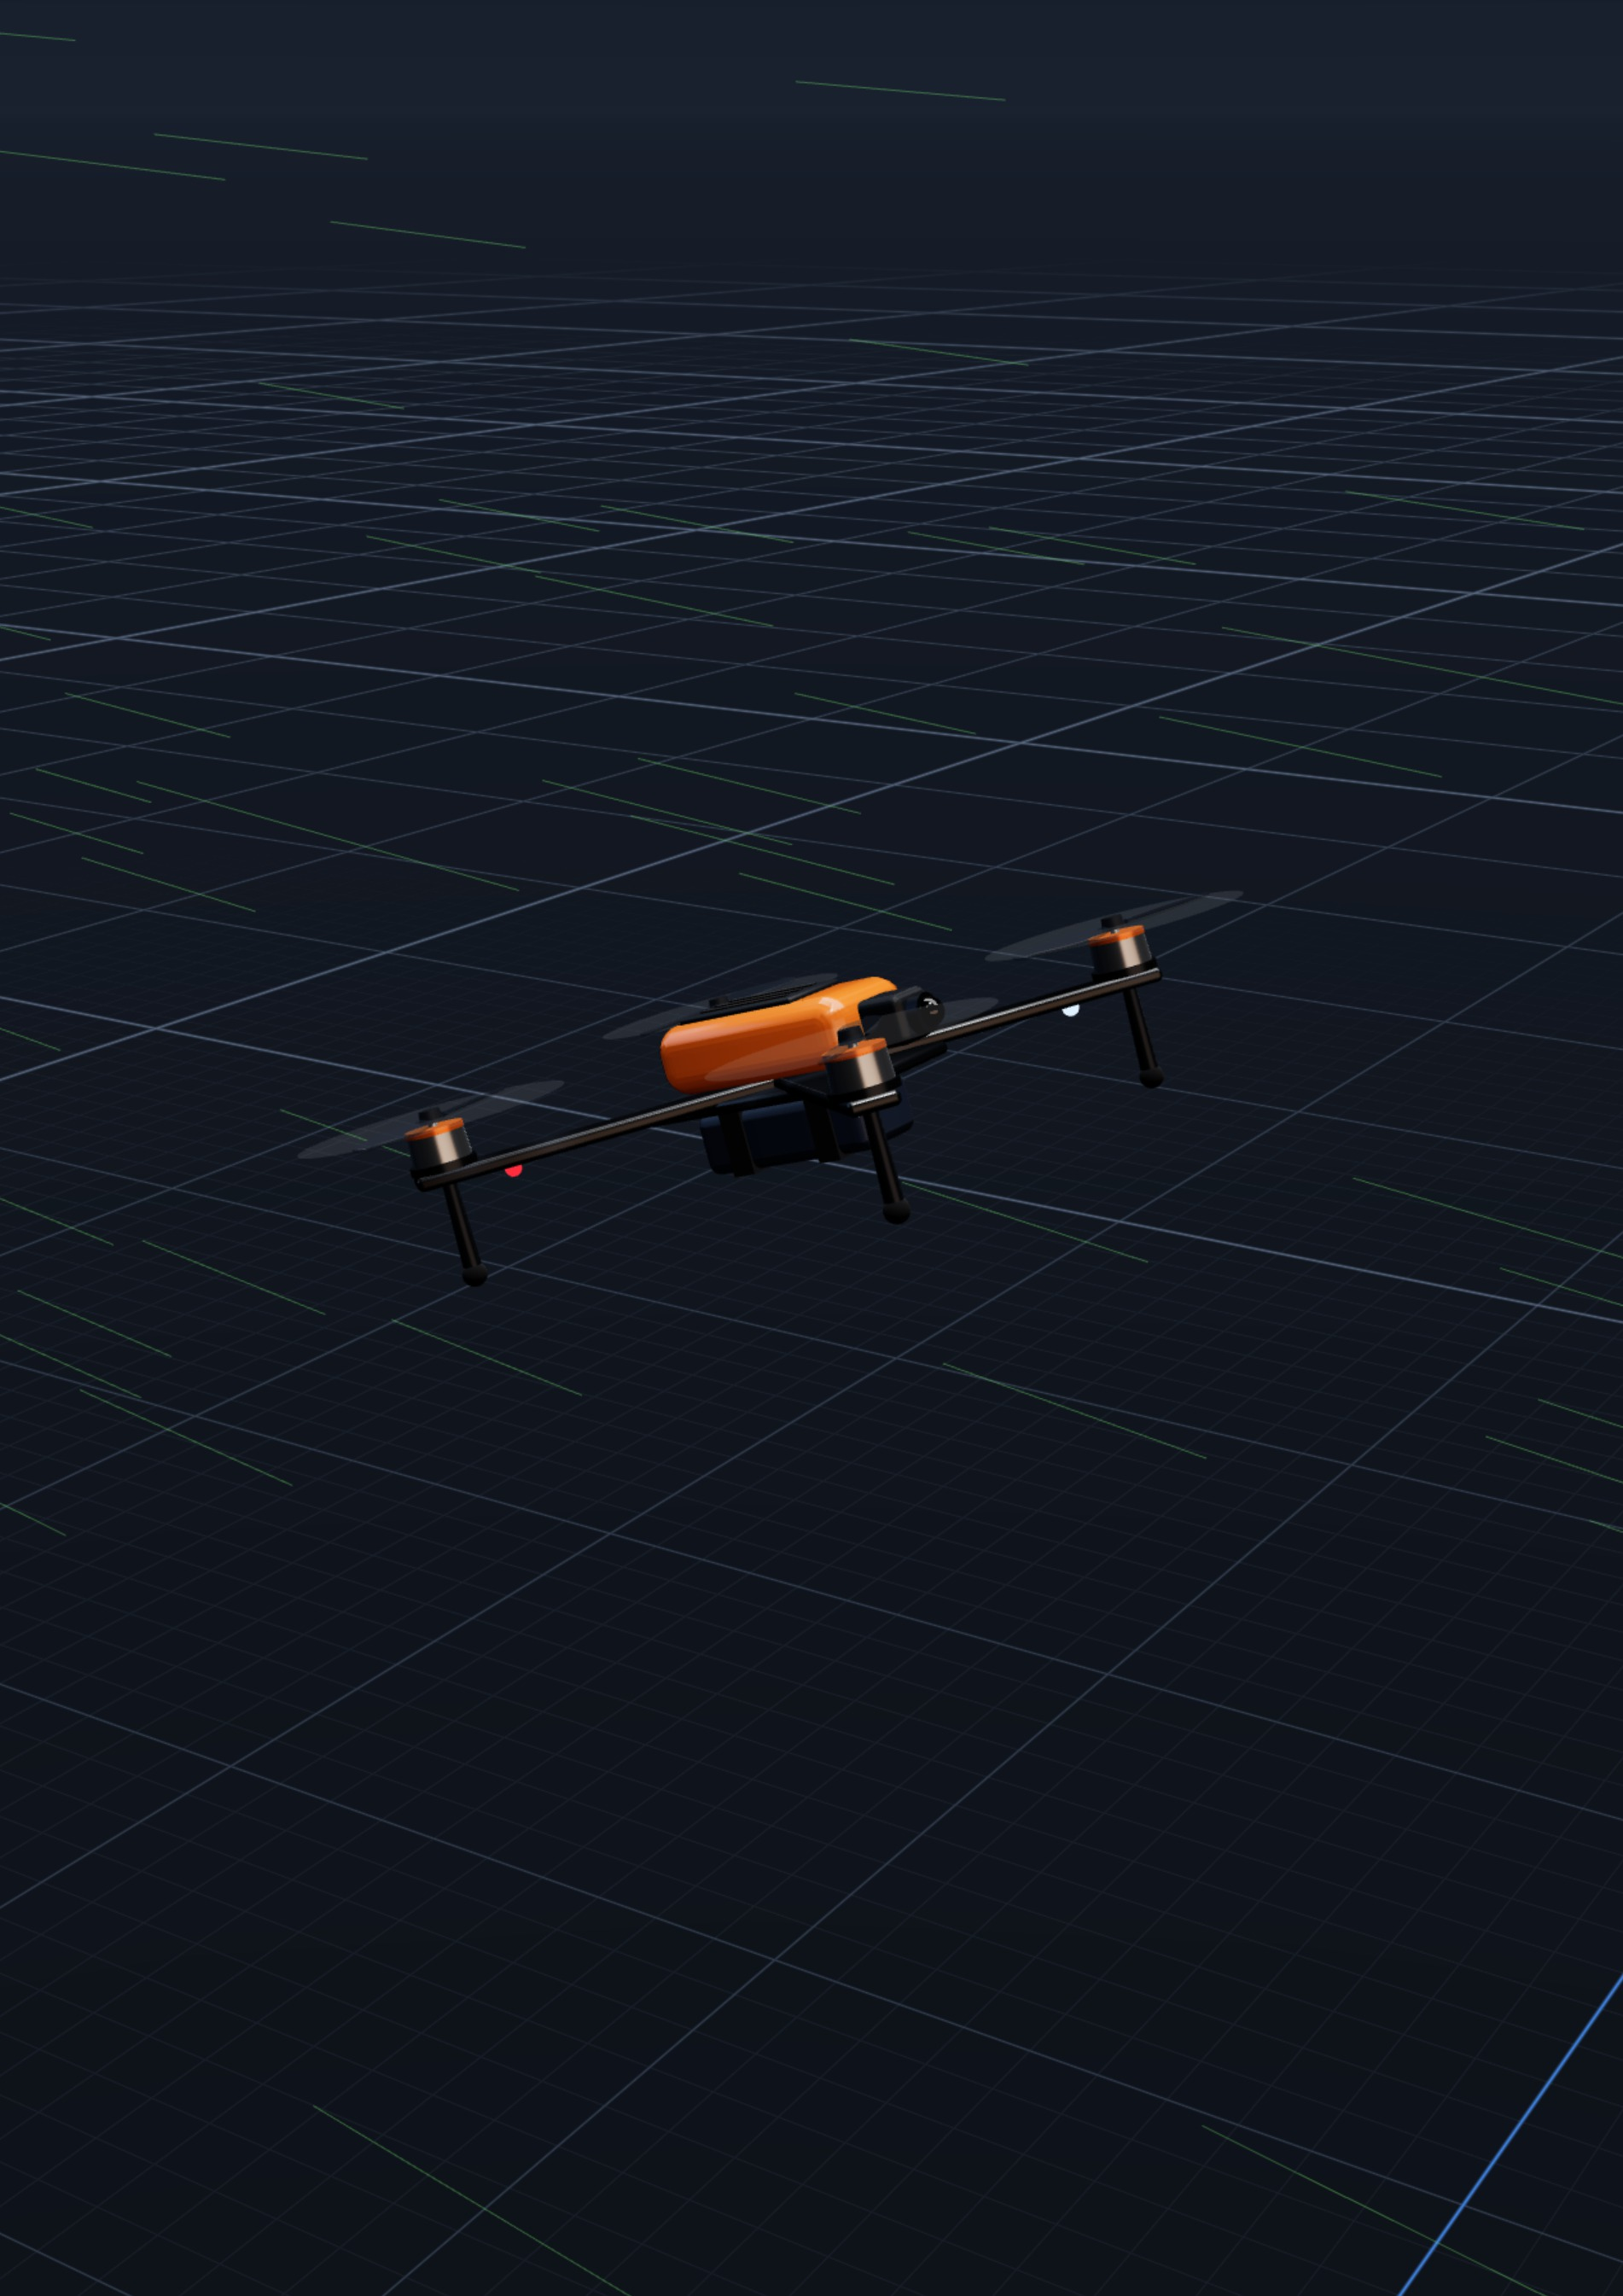
\includegraphics[width=\paperwidth, height=\paperheight]{screens/cover.jpg}};
  \fill[night, path fading=south, opacity=0.92] (current page.north west) rectangle ($(current page.north east)+(0,-120mm)$);
  \fill[night, path fading=north, opacity=0.85] ($(current page.south west)+(0,70mm)$) rectangle (current page.south east);
  \node[anchor=north west, inner sep=0pt, text=accent] at ($(current page.north west)+(24mm,-26mm)$)
    {\appmark\hspace{0.6em}\sanscaps\small A COURSE IN FEEDBACK CONTROL};
  \node[anchor=north west, inner sep=0pt, text=white, inner sep=0pt] at ($(current page.north west)+(23mm,-38mm)$)
    {\parbox[t]{170mm}{\raggedright\nohyph\sansdisplay\fontsize{54}{58}\selectfont Anemostatos}};
  \node[anchor=north west, inner sep=0pt, text=nighttext, inner sep=0pt] at ($(current page.north west)+(24mm,-64mm)$)
    {\parbox[t]{130mm}{\raggedright\displayserif\itshape\fontsize{22}{27}\selectfont Riding on the wind}};
  \node[anchor=north west, inner sep=0pt, text=nightmuted, inner sep=0pt] at ($(current page.north west)+(24mm,-78mm)$)
    {\parbox[t]{130mm}{\raggedright\sffamily\small From PID to learning, with the simulator of the same name}};
  \node[anchor=south west, inner sep=0pt, text=nightmuted, inner sep=0pt] at ($(current page.south west)+(24mm,24mm)$)
    {\parbox[b]{150mm}{\raggedright\sffamily\small The course book of the Anemostatos simulator\\[2pt]
     {\color{nightmuted!70}\footnotesize 35 lessons · 3 levels of flight · every figure flown in the simulator}\\[6pt]
     {\footnotesize Idea and editing: Wojciech Stelmaszewski · Text, figures and code: Claude Opus 5.5}}};
  \node[anchor=south east, inner sep=0pt, text=nightmuted, align=right] at ($(current page.south east)+(-18mm,24mm)$)
    {\displayserif\itshape\small ánemos + statós\\[1pt]{\sffamily\footnotesize “the one that stands in the wind”}};
\end{tikzpicture}
\null\clearpage

% ---------------------------------------------------------------- title page
\thispagestyle{empty}
\vspace*{50mm}
\noindent{\sanscaps\small\color{accent}A COURSE IN FEEDBACK CONTROL}\par\vspace{8mm}
\noindent{\sansdisplay\fontsize{36}{42}\selectfont Anemostatos}\par\vspace{5mm}
\noindent{\displayserif\itshape\fontsize{20}{25}\selectfont Riding on the wind}\par\vspace{7mm}
\noindent{\displayserif\itshape\fontsize{13}{18}\selectfont From PID to learning, with the simulator of the same name}\par
\vspace{24mm}
\noindent\begin{minipage}{118mm}\sffamily\small\color{muted}
Thirty-five lessons, each one a chapter. Every chapter explains one idea step by step, shows it in
numbers flown by the simulator, points to the exact place in the application and its source code
where the idea lives, and ends with a story of the same idea at work in the real world.
\end{minipage}
\par\vspace{16mm}
\noindent\begin{minipage}{118mm}\sffamily\small
{\color{muted}Idea and editing}\\[1pt]{\large Wojciech Stelmaszewski}\par\vspace{5mm}
{\color{muted}Text, figures and code}\\[1pt]{\large Claude Opus 5.5}
\end{minipage}
\vfill
\noindent{\sffamily\footnotesize\color{faint}Edition of 30 September 2026 · written for the simulator at commit \texttt{801cb6b} and later}
\clearpage

% ---------------------------------------------------------------- imprint ---
\thispagestyle{empty}
\vspace*{\fill}
\begin{minipage}{118mm}\sffamily\footnotesize\color{muted}\linespread{1.25}\selectfont
\textbf{\color{ink}Anemostatos: Riding on the wind} — a course in feedback control, with the simulator of the same name.\par\medskip
The idea of the course and the editing of this book are by Wojciech Stelmaszewski. The text, the figures, the
simulator and its source code were written by Claude Opus 5.5, an AI model made by Anthropic
(see the \hyperref[ch:colophon]{colophon}).\par\medskip
The simulator, its lessons and the source code referenced throughout this book live at
\url{https://github.com/wojciech-stelmaszewski/anemostatos}. Start it with \texttt{make dev}; the lesson panel on the right
of the screen follows the same numbering as this book.\par\medskip
Every time series in this book was produced by the simulator itself (\texttt{scripts/book-data.ts}), running the
same code and the same lesson set-ups as the application; the plots were drawn with \texttt{book/tools/make\_figures.py}. Screenshots
come from the running application. Photographs are public domain or under Creative Commons licences; their
authors and licences are listed on page~\pageref{credits}.\par\medskip
Set in Libertinus Serif, Libertinus Math, Fira Sans and Fira Mono with Lua\LaTeX.\par\medskip
\copyright\ 2026. Text and figures may be shared for teaching and learning.
\end{minipage}
\clearpage

\clearpage
\thispagestyle{empty}
{\sffamily\fontsize{27}{31}\selectfont Contents\par}
\vspace{10mm}
\begingroup
\makeatletter\@starttoc{toc}\makeatother
\endgroup

\bookchapter{}{Technical preface}{How the book is built, and how it goes with the simulator.}
\label{ch:preface}

\lead{This book is a companion. It was made together with a simulator, Anemostatos, and the two follow each other step by step: the same lessons, with the same numbers and the same titles, the same experiments, the same colours. The simulator lets you watch a feedback loop work, change it and break it; the book explains what you see. Each is incomplete without the other.}

\section*{A companion to the simulator}
Every chapter of the book is one lesson of the application. A lesson there sets up an experiment — a drone, a controller, a wind, a sensor — and starts it; the chapter here sets up the same experiment and asks what will happen and why. Every time series in the book was flown by the simulator itself, with the same code and the same set-up as the lesson in the application, so a plot on the page and a chart on the screen are two views of one flight. Dark boxes styled like the application say where an idea lives on the screen and in the source code; experiments marked \emph{Try this} send you back to the simulator with a question to answer first. The book can be read without the simulator open, but it was written to be read next to it.

\section*{From the particular to the general}
Control theory has a reputation for being abstract. Its textbooks usually begin with the general — Laplace transforms, transfer functions, pole-zero maps — and come to a real machine late, if at all. This book is built the other way round, and that is its main idea: it goes \emph{from the detail and from practice to the general}.

Every chapter starts from one particular thing that can be watched: one drone, one experiment, one number on the screen — a drone that sags below its setpoint, bounces, overshoots, shakes or flips. Then it asks \emph{why}, and works out the answer for this drone, with its real mass and its real gains, building exactly as much mathematics as the answer needs: no more, but also no less. Only then does it step back. The section \emph{The engineer's view} says the same result in general terms, for any system of the same kind; the subsection \emph{In formal terms} states it exactly, as definitions and theorems with their hypotheses and proofs; and the page \emph{Out in the World} shows the same idea at work in a machine that has nothing to do with drones. The particular comes first, and the general is reached from it.

The whole book has the same shape. Part~I builds the PID controller on a drone that can only move up and down, one term and one practical problem at a time, and arrives at a full quadrotor only in its last lessons. Part~II steps up to the general language of states, models and optimisation, once the reader has seen why PID alone is not enough. The later parts of the course, on analysis and on aerospace guidance and control, take the same ideas further still. Theory always arrives when practice has asked for it.

\section*{Who it is for}
The book assumes what a bachelor's degree in engineering, physics, mathematics or computer science usually provides: calculus of one and several variables, the basics of ordinary differential equations (linear equations with constant coefficients, above all), linear algebra (matrices, eigenvalues), and a little probability. Everything beyond that — Laplace transforms, the phase margin, the Riccati equation, the Kalman filter, quadratic programming, quaternions — is introduced where it is first needed, and summarised in \hyperref[app:math]{the mathematical toolbox} at the end.

\section*{How it is organised}
The book follows the lessons of the simulator, one lesson per chapter, with the same numbers and titles you see in the application's lesson panel.
\begin{description}[leftmargin=0pt, font=\sffamily\small\bfseries]
  \item[Part I · PID] (Lessons I.1–I.14) builds the PID controller term by term on a drone that can only move up and down, meets the practical problems of a real digital controller — saturation, windup, derivative kick, noise, sampling, delay, actuator lag — and ends with the cascade of loops that flies a full quadrotor.
  \item[Part II · Beyond PID] (Lessons II.1–II.21) is a second semester in five chapters: optimal state feedback and estimation (LQR, Kalman filter), disturbance observers and incremental control (ADRC, INDI), geometry and trajectories (rotations, differential flatness, minimum-snap planning), optimisation in the loop (MPC, MPPI, control barrier functions), and adaptation and learning (L1 adaptive control, learned models, neural-network policies) — ending with a comparison of all of them on equal terms.
\end{description}
These two parts are the first volume of a longer course. Part~III, \emph{Why it works}, turns from design to analysis: frequency response, stability margins, Lyapunov's method, robustness, estimation with real sensors, and verification by Monte Carlo. Part~IV, \emph{Aerospace GNC}, takes the same ideas to a rocket, an aircraft and a satellite and adds optimal control from first principles, gain scheduling and guidance. Part~V is about engineering practice. Their lessons appear in the simulator first and in later volumes of this book; the \hyperref[ch:colophon]{colophon} says where to find the plan.

Chapter~0, \hyperref[ch:intro]{\emph{Why control?}}, tells how this book began — with a small helicopter on Mars — and then introduces the field itself: what control theory is, how it is organised, where it is used and where it came from. The \hyperref[ch:prelude]{Prelude} then introduces the simulator and its physics. Read both first, or come back to the Prelude when a lesson refers to it.

\section*{The anatomy of a lesson}
Every chapter has the same parts, set in the same way throughout the book:

\begin{keyidea}[the one thing to take away]
Boxes like this state the central idea of a section in a few sentences.
\end{keyidea}
\begin{definition}{a precise term}
Definitions fix the vocabulary.
\end{definition}
\begin{inapp}[where the idea lives in the application]
These dark boxes, styled like the application itself, say where to find an idea on the screen — \ui{Group\then Parameter} — which parameter (\param{control.alt.kp}) and which source file (\src{src/control/pid.ts}) implement it, and which keys to press (\key{R}). File names are links to the repository.
\end{inapp}
\begin{trythis}
Experiments to run in the simulator, usually with a question to answer \emph{before} running them.
\end{trythis}
\begin{watchout}
Common mistakes and the limits of a result.
\end{watchout}
\begin{example}[a problem solved in full]
Worked examples take a concrete question with the drone's real numbers and solve it step by step, with nothing left out. They are the backbone of each lesson: read them with a pencil.
\end{example}
\begin{lookahead}[the thread into the rest of the course]
A lesson closes its theory with a section \emph{The engineer's view}, which says the result again in the language used at work — state, poles, energy — and ends with a subsection \emph{In formal terms}, where the definitions and theorems are stated exactly, with their hypotheses and a proof or its source. Then comes a box like this one, which names the later lessons where the idea returns.
\end{lookahead}
Two more things recur. Wherever a formula predicts a number, a figure or a table puts the prediction next to what the simulator measured, and the text explains any difference. And each chapter ends with a page \emph{Out in the World} — the same idea at work somewhere else, with a photograph — a short summary, and exercises marked by difficulty ({\tiny$\bullet$} to {\tiny$\bullet\bullet\bullet$}). Some exercises carry a label in the margin: \exkindinline{derive} asks for a derivation with pencil and paper, \exkindinline{fly} for an experiment in the simulator, and \exkindinline{code} for reading or changing the simulator's source. The margin of a lesson's first page holds its set-up: what is switched on, and what happens when. Complete solutions of the exercises will be published in a companion volume.

\section*{One colour, one meaning}
The simulator gives every quantity its own colour, in its charts, its 3D view and its parameter panel. This book uses the same colours, so that a figure here and a chart on the screen read the same way:

\begin{center}\small\sffamily
\begin{tabular}{@{}lll@{\hspace{2.5em}}lll@{}}
  \textcolor{sigsp}{\rule[0.5ex]{1.2em}{1.2pt}} & setpoint $r$ & dashed grey &
  \textcolor{sigP}{\rule[0.3ex]{1.2em}{2pt}} & \Pt term & orange\\
  \textcolor{sigmeas}{\rule[0.3ex]{1.2em}{2pt}} & measurement $y$ & blue &
  \textcolor{sigI}{\rule[0.3ex]{1.2em}{2pt}} & \It term & green\\
  \textcolor{sigerr}{\rule[0.3ex]{1.2em}{2pt}} & error $e$ & red &
  \textcolor{sigD}{\rule[0.3ex]{1.2em}{2pt}} & \Dt term & violet\\
  \textcolor{sigwind}{\rule[0.3ex]{1.2em}{2pt}} & wind & green &
  \textcolor{sigFF}{\rule[0.3ex]{1.2em}{2pt}} & \FFt (feedforward) & amber\\
\end{tabular}
\end{center}
Red shading in a time plot means that an actuator is saturated, as in the application.

\section*{Where the numbers come from}
All time series in this book were produced by the simulator itself. A script, \src{scripts/book-data.ts}, sets up each lesson exactly as the application does, flies it headlessly with the same code, and records the telemetry; the figures are drawn from those recordings. When a number in the text says \enquote{the simulator shows \SI{0.45}{m}}, you can reproduce it. Where theory and simulation disagree — and they sometimes do, instructively — the book says so and explains why.

\section*{Running the simulator}
Anemostatos runs locally in a web browser. With Node.js installed:
\begin{center}
\texttt{git clone https://github.com/wojciech-stelmaszewski/anemostatos}\\
\texttt{cd anemostatos \&\& make dev}
\end{center}
The lesson panel on the right of the screen has two tabs, \ui{Part I · PID} and \ui{Part II · Beyond PID}; select a lesson and press \ui{Start}. Everything else — every gain, every physical parameter, the wind, the sensors — stays unlocked: the lessons are starting points, not rails.


\mainmatter
\bookchapter{0}{Why control?}{How this book began — with a helicopter on Mars — and what control theory is, where it came from and why a drone is the place to learn it.}
\label{ch:intro}

\lead{This book began on Mars. On 19~April 2021 a helicopter not much bigger than a toy lifted itself off the ground of another planet, hovered for half a minute and landed again. I watched it happen, and it fascinated me completely. This chapter tells that story first. Then it says what control theory is — the science that made the flight possible, and the subject of this book.}

\section{A helicopter on Mars}\index{Ingenuity (Mars helicopter)}

I followed the flights of Ingenuity, NASA's helicopter on Mars, as the news of each one arrived, and I was completely taken by them. It is hard to say how strongly a piece of engineering can move a person, but this one moved me. A machine of less than two kilograms, made by people, flying by itself through the thin air of a world where no person has ever stood — and doing it not once, as planned, but again and again. What I felt most was admiration: for the people who built it, and above all for the quiet power of the thing that kept it in the air, its control system. That admiration is the reason this book exists.

\sidecapfig{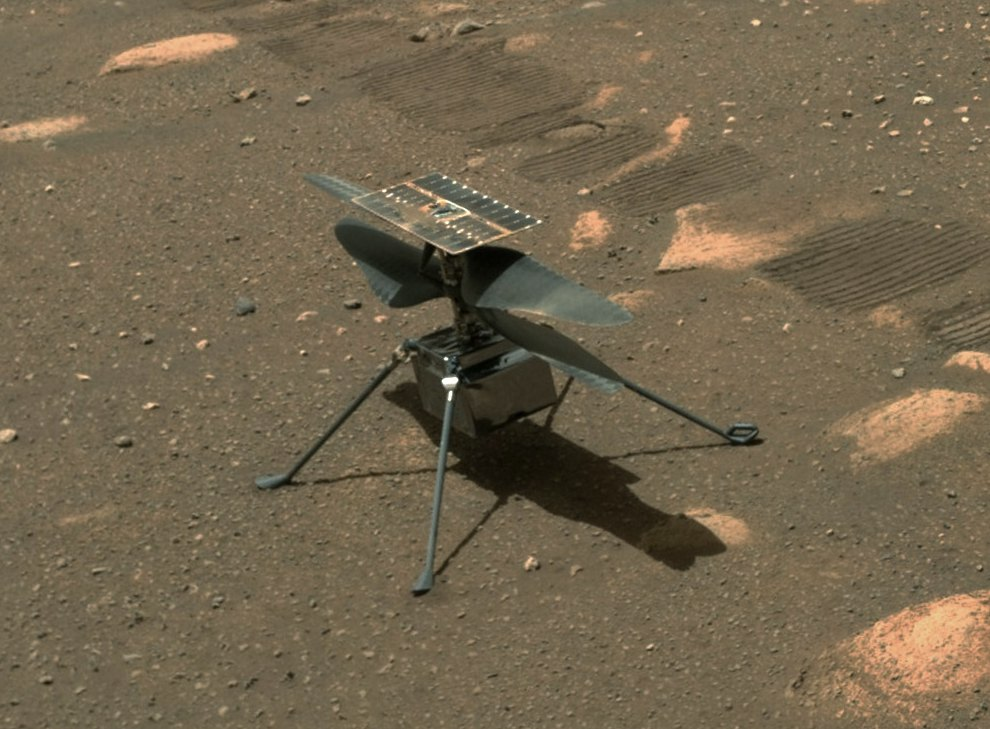
\includegraphics[width=\linewidth]{photos/ingenuity-mars}}
  {Ingenuity on the floor of Jezero crater, April 2021, photographed by the Perseverance rover. The two rotors, \SI{1.2}{m} across, turn in opposite directions; the solar panel on top charges its batteries. \hyperref[credit:ingenuity-mars]{\textsc{credit}}}
  {fig:intro-ingenuity}

Ingenuity reached Mars on 18~February 2021, folded under the belly of the Perseverance rover, which landed in Jezero crater. In early April the rover set it down on the ground (Figure~\ref{fig:intro-ingenuity}) and drove away, and the helicopter had to survive its first freezing night alone, on the power of its own small solar panel.

The engineering problem was extreme. The atmosphere of Mars has less than one per cent of the density of the air on Earth: a rotor there pushes against almost nothing. Ingenuity's answer was a pair of rotors \SI{1.2}{m} across, turning in opposite directions at about 2400 revolutions per minute, above a body of \SI{1.8}{kg}. And nobody could fly it. A radio signal needs several minutes to travel between Earth and Mars, up to about twenty-two, so there could be no pilot with a joystick, not even a patient one. Ingenuity had to fly itself. A camera looking down at the ground and inertial sensors told it where it was and how it was moving, and a computer built around a processor designed for smartphones closed the loop, many times every second, from sensors to rotors and back.

The first flight came on 19~April 2021. The helicopter rose about three metres, hovered and came down again, some thirty-nine seconds in all: the first powered, controlled flight of an aircraft on another planet. The patch of ground it flew from was named Wright Brothers Field, and the helicopter carried a small piece of the fabric that had covered the wings of the Wright brothers' Flyer in 1903.\marginphoto{ingenuity-wright}{The swatch of Wright Flyer fabric that flew on Ingenuity, photographed at JPL before launch.} Its own navigation camera took the first picture of Figure~\ref{fig:intro-shadows}: its shadow on the ground of Mars.

Ingenuity was meant to make at most five flights in thirty days, to show that flight on Mars was possible at all. It made seventy-two, over almost three years. It flew for 128.8~minutes in total, covered \SI{17}{km}, climbed as high as \SI{24}{m}, reached \SI{10}{m/s}, and became a scout for the rover, looking ahead at the ground it would have to cross.

\begin{figure}[tbp]
  \noindent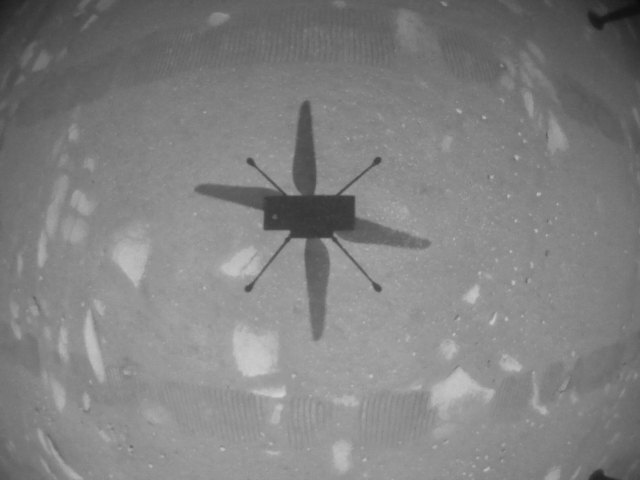
\includegraphics[height=40mm]{photos/ingenuity-shadow}\hfill
  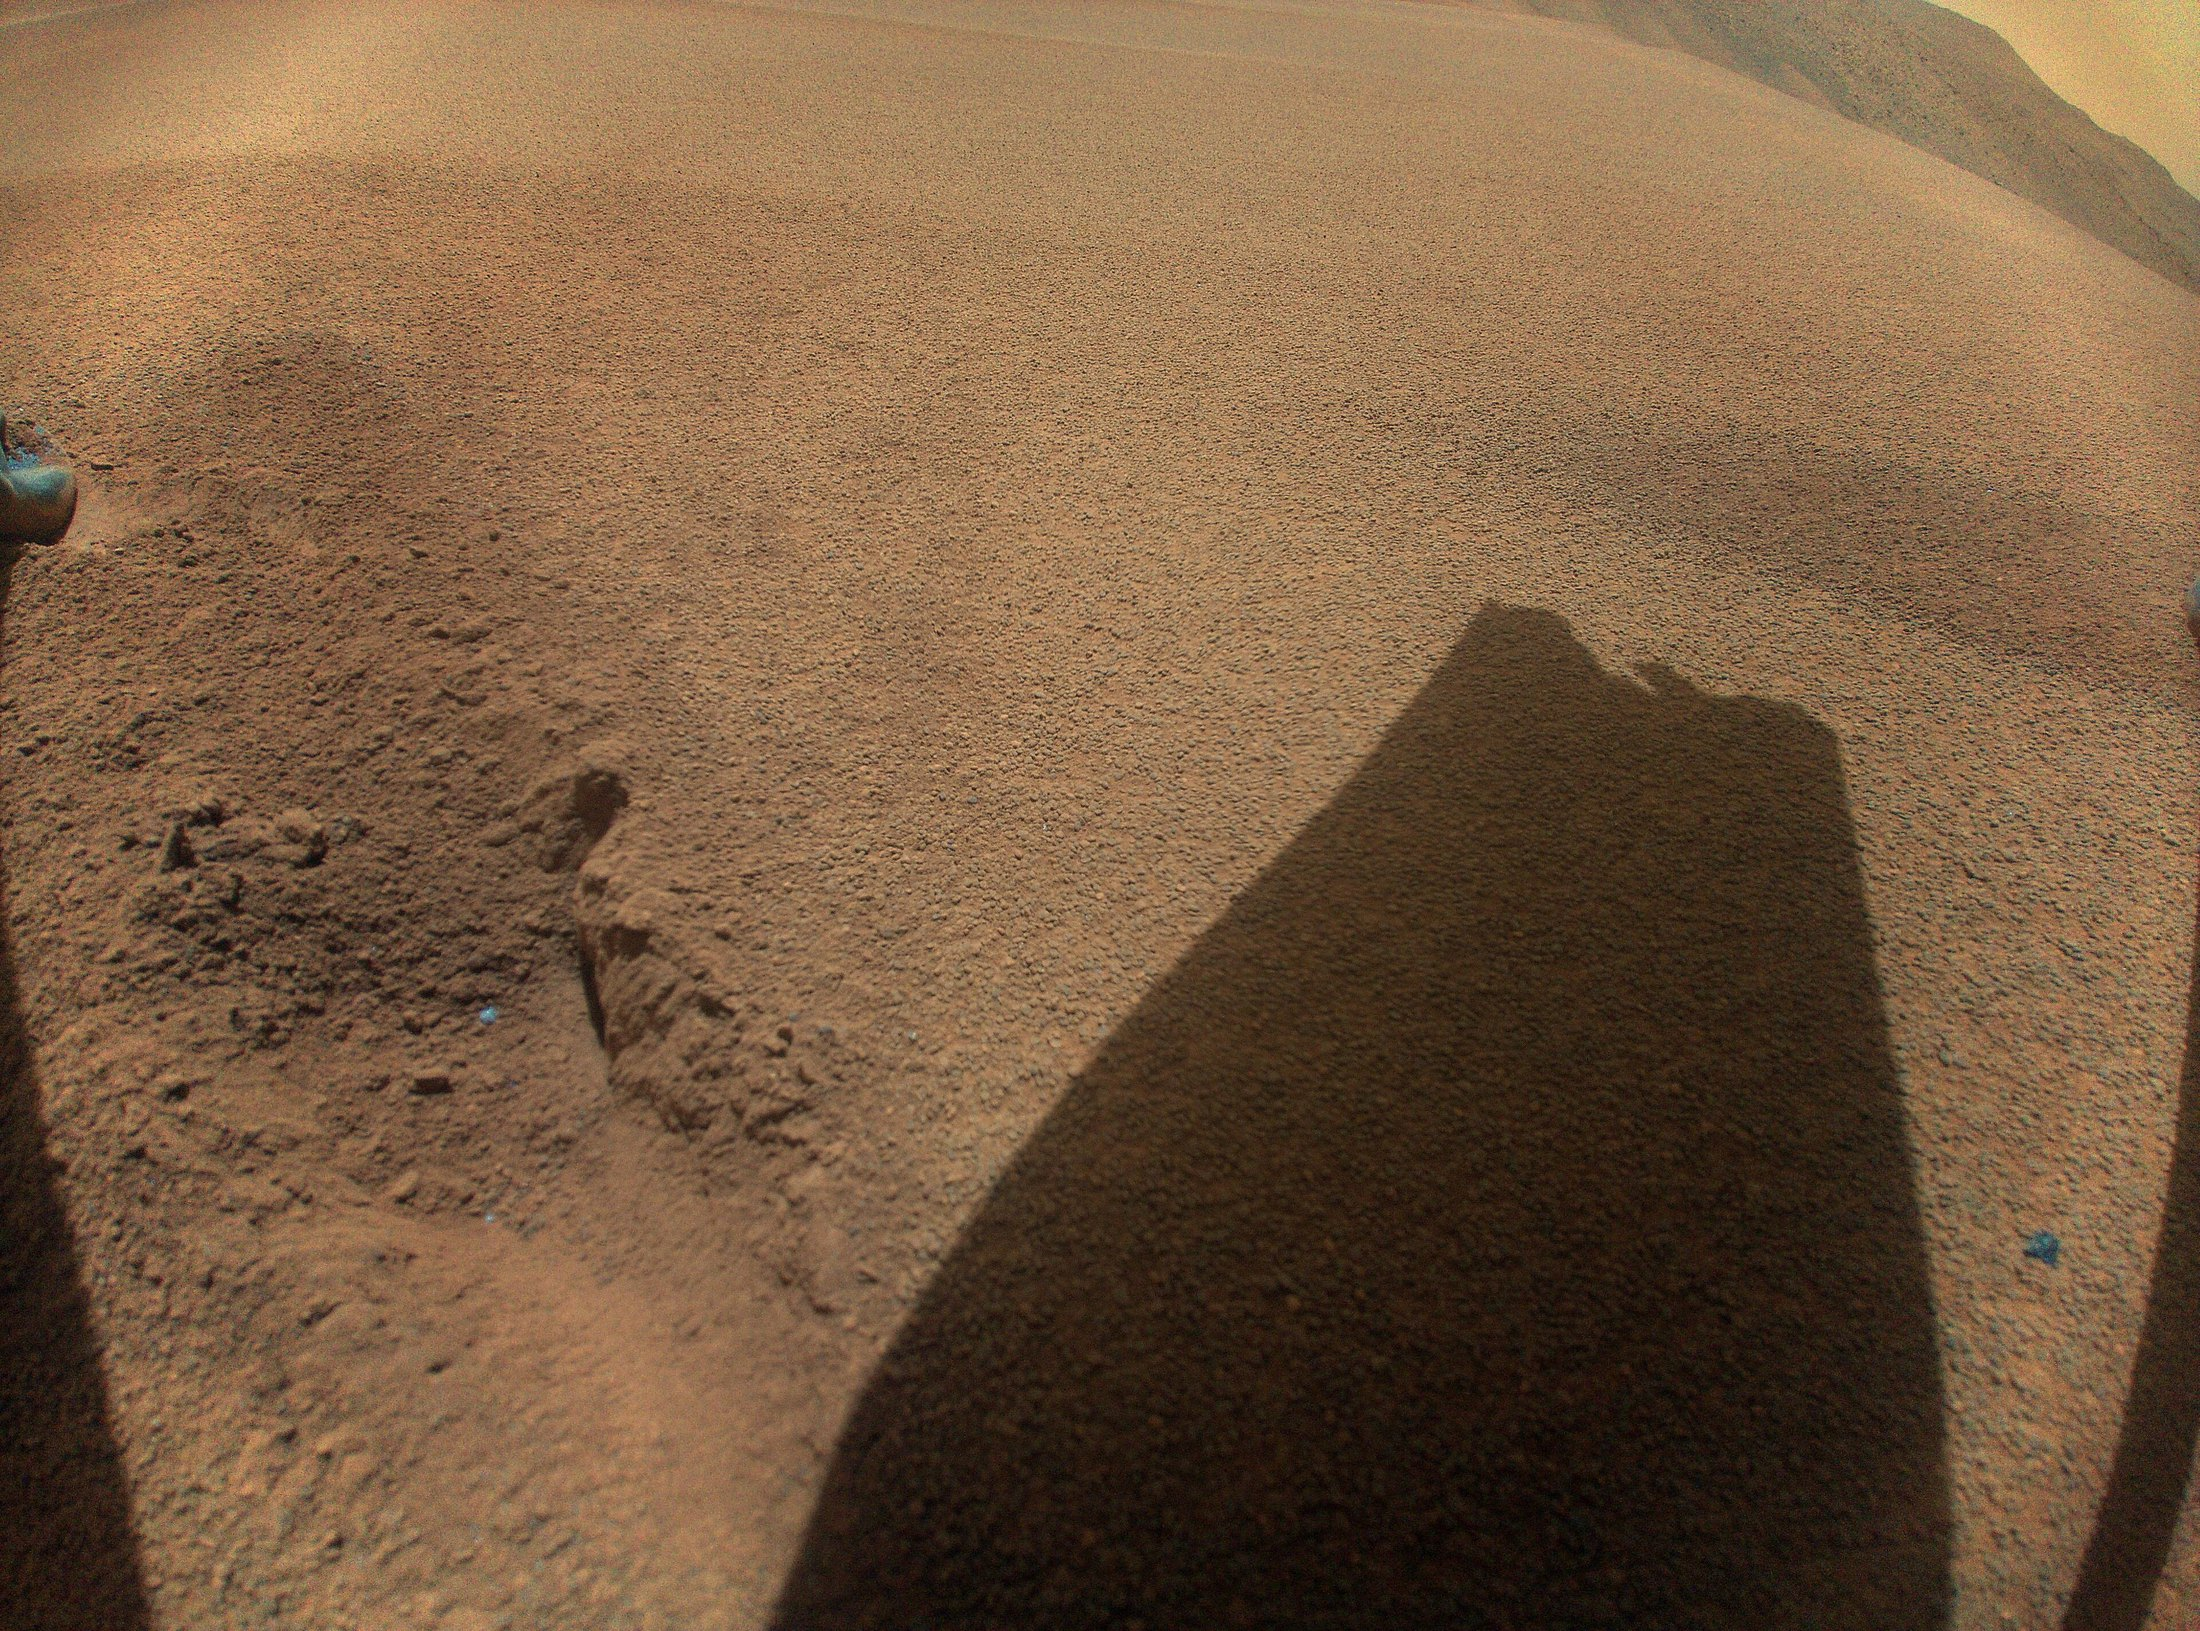
\includegraphics[height=40mm, trim=0 0 0 205, clip]{photos/ingenuity-blade}
  \captionsetup{style=sidecaption}
  \caption{Two pictures taken by Ingenuity's own camera, almost three years apart. Left: its shadow during the first flight, 19~April 2021. Right: the shadow of a broken rotor blade after the seventy-second and last, 18~January 2024. \hyperref[credit:ingenuity-shadow]{\textsc{credit}}, \hyperref[credit:ingenuity-blade]{\textsc{credit}}}
  \label{fig:intro-shadows}
\end{figure}

The flight I think of most is the sixth, on 22~May 2021. Fifty-four seconds after take-off a single image from the navigation camera was lost, and from then on every image arrived with the wrong time attached. The navigation kept \enquote{correcting} errors that did not exist. The helicopter began to tilt back and forth, with roll and pitch swings of more than twenty degrees, large commands to the rotors and spikes in power. It did not fall. It flew the rest of its route and landed about five metres from the planned spot. Its chief pilot, Håvard Grip, explained why a few days later:
\begin{quote}\itshape
We designed Ingenuity to tolerate significant errors without becoming unstable, including errors in timing. This built-in margin was not fully needed in Ingenuity's previous flights, because the vehicle's behavior was in-family with our expectations, but this margin came to the rescue in Flight Six.
\end{quote}
A margin — of stability, against errors nobody had foreseen — saved a machine hundreds of millions of kilometres from the nearest engineer. Much of this book is about what such a margin is and how to build one.

The seventy-second flight, on 18~January 2024, was the last. The helicopter crossed a stretch of smooth, featureless sand, where its navigation had little to track; on landing at least one rotor blade broke (Figure~\ref{fig:intro-shadows}, right). On 25~January NASA announced that the mission was over. Ingenuity still stands where it came down.

\section{From Mars to this book}

What kept Ingenuity in the air was not only its rotors, its batteries and its light carbon body. It was a loop: measure where you are, compare it with where you should be, act on the motors — and do it again, many times a second, faster than anything can go wrong. That loop is what this book is about, and almost every lesson in it is a piece of what Ingenuity had to do.

To hover, a rotorcraft must hold its height against gravity with a thrust it adjusts all the time; that is where the book starts (\lessonref{les:meet} to \lessonref{les:integral}). It must do it with motors that have limits, sensors that are noisy and a computer that looks at the world in snapshots (\lessonref{les:windup} to \lessonref{les:slow}). To move, or simply to stand still in a wind, it must tilt (\lessonref{les:tilt}), and so its loops are nested: a fast loop for its attitude inside a slower one for its position (\lessonref{les:cascade}). It must work out where it is from a camera and inertial sensors, none of which can be trusted alone (\lessonref{les:kalman}). And when something unforeseen happens — a lost image, a wrong timestamp — it must stay stable anyway, because its designers left a margin (\lessonref{les:edge}, and the whole of Part~III).

The drone of this book is a small cousin of Ingenuity. It has four rotors instead of two, and it flies not on Mars but in a simulator on your screen, where every experiment can be repeated, changed and broken without losing a spacecraft. The problems, though, are the same, and so are the ideas that solve them. My hope is that by the end of the book the reader will understand, in principle, how a machine like Ingenuity keeps itself in the air — and share a little of the admiration I felt watching it fly.\par
\smallskip
{\raggedleft\sffamily\small\color{muted}— Wojciech Stelmaszewski\par}

\section{What control is}

Look around you. The room you sit in is held at a comfortable temperature. Your body keeps its own temperature at \SI{37}{\celsius} whether you are in the sun or in the snow. The electricity in the socket arrives at 50 or \SI{60}{Hz}, never mind how many kettles were just switched on. A camera holds its picture still in a shaking hand. None of this happens by itself. Behind each of these facts is a \emph{control system}: something that measures, compares and acts, over and over again. This chapter is about the science of such systems.


Most of the physical world, left to itself, drifts. A room cools down, an engine speeds up when the load is removed, a pencil standing on its tip falls over. Engineering is very often the art of making such things behave the way we want them to, although we cannot know in advance everything that will happen to them.

\begin{definition}{Control}
\term{Control} is the act of choosing the inputs of a system so that its behaviour meets a goal, despite uncertainty about the system and about the influences acting on it. The system being controlled is called the \term{plant}; the device or algorithm that chooses the inputs is the \term{controller}.
\end{definition}

Every control problem has three ingredients:
\begin{enumerate}
  \item \textbf{a goal} — keep a temperature at \SI{21}{\celsius}, a car at \SI{100}{km/h}, a drone at \SI{2}{m};
  \item \textbf{a way to act} — a heater, a throttle, four motors (the \term{actuators});
  \item \textbf{uncertainty} — an open window, a hill, a gust of wind; and a model of the plant that is never quite right.
\end{enumerate}
Without the third ingredient there would be no subject. If we knew the plant exactly and nothing unexpected ever happened, we could compute the right inputs once, in advance, and simply play them back. Control theory exists because the world is uncertain.\didyouknow{The word \emph{plant} comes from the process industry: the first control engineers regulated chemical and power plants, and the name stayed — even when the plant is a drone, a patient or an economy.}

\subsection{Two ways to act: open loop and closed loop}
There are two fundamentally different ways to choose the inputs.

\begin{definition}{Open-loop and closed-loop control}
In \term{open-loop} control the input is computed from the goal and a model alone; the result is never checked. In \term{closed-loop} (\term{feedback}) control the result is measured by a \term{sensor}, compared with the goal, and the difference — the \term{error} — is used to correct the input continuously.
\end{definition}

A toaster is open-loop: it heats for a fixed time and never looks at the bread. Whether the toast comes out pale or burnt depends on the bread, the voltage and the starting temperature, and the toaster cannot tell. A thermostat is closed-loop: it measures the room temperature, compares it with the setting and switches the heater accordingly. Open the window, and the thermostat responds, without knowing that a window exists.\tip{To tell the two apart, ask one question: does the device look at the result? If it does not, it is open-loop, however clever its plan.}

\subsection{What feedback buys — and what it costs}
Feedback has four remarkable properties, and every one of them appears in this book.
\begin{enumerate}
  \item \textbf{It rejects disturbances it cannot see.} A controller reacts to the \emph{effect} of a disturbance, the error, so it does not need to know the cause (\lessonref{les:meet}).
  \item \textbf{It makes a system insensitive to its own imperfections.} This is less obvious and very important; the worked example below makes it concrete.
  \item \textbf{It can stabilise what is unstable.} A drone, a rocket balancing on its engine, a fighter jet designed to be unstable: none of them can stay up without feedback (\lessonref{les:edge}).
  \item \textbf{It can shape the behaviour} — speed, smoothness, damping — almost at will, by the choice of the controller.
\end{enumerate}
It also has costs. A feedback loop reacts only \emph{after} an error has appeared.\pitfall{The sign matters. Reverse the correction and the same loop pushes the error \emph{away} from zero. A microphone held close to its own loudspeaker howls for this reason.} It feeds the sensor's noise into the actuators (\lessonref{les:noise}). And, most importantly, a badly designed feedback loop can itself make a stable system oscillate or diverge: the Watt governors that \enquote{hunted}, and the bridge of \lessonref{les:spring}. Understanding exactly when feedback helps and when it harms is the core of control theory.

\begin{example}[Feedback makes an amplifier precise]
\label{ex:intro-black}
In 1927 the telephone engineer Harold Black\index{feedback amplifier}\index{Black, Harold} faced a problem: the vacuum-tube amplifiers of long-distance lines had a gain that drifted with temperature and age, and every drift distorted the calls. His solution was feedback, and a short calculation shows why it works.

\textbf{Step 1 — the open-loop amplifier.} Suppose an amplifier has a gain $A = 1000$, but, because of its tubes, the gain may vary by $\pm20\,\%$: anywhere between 800 and 1200. The output is $v_{out} = A\,v_{in}$, so the output varies by $\pm 20\,\%$ as well.

\textbf{Step 2 — close the loop.} Feed a fraction $\beta$ of the output back and subtract it from the input, using a precise resistor divider with $\beta = 0.1$.\didyouknow[-112pt]{Black had the idea on the ferry to work on 2~August 1927 and sketched it on his copy of \emph{The New York Times}. The patent took nine years to be granted: throwing gain away to gain precision sounded absurd.} The amplifier now amplifies the difference:
\begin{equation*}
  v_{out} = A\,(v_{in} - \beta\,v_{out}).
\end{equation*}

\textbf{Step 3 — solve for the closed-loop gain.} Collect $v_{out}$ on the left: $v_{out}(1 + A\beta) = A\,v_{in}$, so
\begin{equation*}
  G = \frac{v_{out}}{v_{in}} = \frac{A}{1 + A\beta}.
\end{equation*}

\textbf{Step 4 — put in the numbers.} For $A = 1000$: $G = 1000/101 = 9.901$. For $A = 800$: $G = 800/81 = 9.877$. For $A = 1200$: $G = 1200/121 = 9.917$.

\textbf{Step 5 — interpret.} The gain has dropped from 1000 to about 10, but its variation has dropped from $\pm20\,\%$ to about $\pm0.2\,\%$ — a hundred times smaller. When $A\beta \gg 1$, $G \approx 1/\beta$: the gain is set by the precise resistors, not by the imprecise tubes. We have traded raw gain for accuracy.\tip{A rule to keep: feedback divides every imperfection inside the loop by the loop gain. Here $1 + A\beta = 1 + 1000 \cdot 0.1 = 101$.} The factor $1 + A\beta$, by which the sensitivity drops, is called the \emph{loop gain}, and it will appear again and again, from \lessonref{les:droop} onwards.
\end{example}

\section{How control theory is organised}

Control theory is a large field, but its structure is simple. It follows the workflow of every control project (\cref{fig:intro-map}, top):
\begin{enumerate}
  \item \textbf{Modelling.} Write down equations that describe the plant well enough — Newton's laws for a drone, heat balances for a room, chemical kinetics for a reactor. Or measure the plant and fit a model to the data (\emph{system identification}).
  \item \textbf{Analysis.} Ask what the plant, and the plant with a given controller, will do: Is it stable? How fast does it respond? How much does a disturbance move it? How much can the model be wrong before things go bad?
  \item \textbf{Design.} Choose the controller so that the answers to these questions are acceptable. This is where the many families of methods differ.
  \item \textbf{Implementation.} Turn the design into something that runs: on a computer, at a finite sampling rate, with real sensors and actuators that are noisy, delayed and limited. Then test it — in simulation first — and go back to step 1 when reality disagrees.\didyouknow{Ask a practising control engineer where the time goes: mostly into modelling and testing. The control law itself is often a few dozen lines of code.}
\end{enumerate}

\begin{figure}[t]
\begin{fullwidth}
  \centering% A map of control theory: the workflow (top) and the families of methods (below), with the course's lessons.
\begin{tikzpicture}[
  every node/.style={font=\sffamily\footnotesize},
  wfstep/.style={draw=ink, line width=0.6pt, rounded corners=2pt, fill=white, minimum height=12.5mm, text width=33.2mm, align=center, inner sep=3pt},
  fam/.style={draw=#1, line width=0.6pt, rounded corners=2pt, fill=#1!7, text width=48.9mm, align=left, inner sep=5pt,
    minimum height=25mm, anchor=north west},
]
  % workflow: four equal steps across the full width
  \node[wfstep, anchor=north west] (m) at (0,0) {\textbf{Model}\\{\scriptsize\color{muted}equations of the plant}};
  \node[wfstep, anchor=north west] (a) at (43.5mm,0) {\textbf{Analyse}\\{\scriptsize\color{muted}stability, speed, margins}};
  \node[wfstep, anchor=north west] (d) at (87mm,0) {\textbf{Design}\\{\scriptsize\color{muted}the control law}};
  \node[wfstep, anchor=north west] (i) at (130.5mm,0) {\textbf{Implement and test}\\{\scriptsize\color{muted}sample, filter, saturate}};
  \draw[sig] (m) -- (a); \draw[sig] (a) -- (d); \draw[sig] (d) -- (i);
  \draw[sig, faint] (i.north) -- ++(0,4mm) -| node[pos=0.25, above, lab] {not good enough? iterate} (m.north);
  % families: two rows of three, tops and heights aligned
  \node[font=\sffamily\scriptsize, text=muted, anchor=south west, inner sep=0pt] at (0,-21mm) {families of methods — each answers the design question differently};
  \node[fam=sigP]     at (0,-23mm)       {\textcolor{sigP}{\textbf{Classical}}\\ PID, frequency response, Bode and Nyquist, root locus\\[2pt]{\color{muted}Lessons 1–14}\\{\color{faint}later: III.1–III.6}};
  \node[fam=deepblue] at (56.67mm,-23mm)    {\textcolor{deepblue}{\textbf{State space}}\\ state feedback, observers, LQR, Kalman filter\\[2pt]{\color{muted}Lessons II.1–II.4}\\{\color{faint}later: III.9–III.10}};
  \node[fam=sigI]     at (113.33mm,-23mm)   {\textcolor{sigI}{\textbf{Nonlinear and geometric}}\\ Lyapunov, dynamic inversion, rotations, flatness\\[2pt]{\color{muted}Lessons II.7–II.12}\\{\color{faint}later: III.7–III.8}};
  \node[fam=sigD]     at (0,-52mm)       {\textcolor{sigD}{\textbf{Optimal and predictive}}\\ Pontryagin, dynamic programming, MPC\\[2pt]{\color{muted}Lessons II.2, II.13–II.17}\\{\color{faint}later: IV.1–IV.6}};
  \node[fam=sigFF]    at (56.67mm,-52mm)    {\textcolor{sigFF}{\textbf{Robust and adaptive}}\\ disturbance observers, ADRC, L1 adaptive, $H_\infty$\\[2pt]{\color{muted}Lessons II.5–II.6, II.18}\\{\color{faint}later: III.11–III.17}};
  \node[fam=sigerr]   at (113.33mm,-52mm)   {\textcolor{sigerr}{\textbf{Learning-based}}\\ learned models, reinforcement learning, neural policies\\[2pt]{\color{muted}Lessons II.19–II.21}\\{\color{faint}later: III.29–III.30}};
\end{tikzpicture}

  \caption{A map of control theory. Top: the workflow that every control design follows. Below: the main families of design methods, roughly in the order they were developed, with the lessons of this book in which they appear. The fainter line names the lessons of Parts~III and~IV, in later volumes, that return to each family.}
  \label{fig:intro-map}
\end{fullwidth}
\end{figure}

The families of design methods in \cref{fig:intro-map} are not rival schools; they are layers, each added when the previous ones reached their limits.
\begin{description}[leftmargin=0pt, itemsep=3pt, font=\sffamily\small\bfseries]
  \item[Classical control] (1920s–1950s) works with one input and one output and describes systems by how they respond to sinusoids of different frequencies. Its workhorse, the PID controller, still runs the vast majority of the world's control loops.\innumbers{Surveys of process plants find that more than nine loops in ten are PID — and most of those are really PI, with the D term switched off.} Part~I of this book.
  \item[State-space control] (from 1960) describes a system by a vector of internal variables, its \emph{state}, and handles many inputs and outputs at once with linear algebra. It brought optimal control (LQR) and optimal estimation (the Kalman filter).
  \item[Nonlinear and geometric control] deals with systems whose equations cannot be linearised usefully — large rotations, for example, which matter for every aircraft and drone.
  \item[Optimal and predictive control] states the goal as a cost to be minimised and computes the control by optimisation, often online, while respecting limits such as maximum thrust or forbidden regions.
  \item[Robust and adaptive control] designs controllers that keep working when the model is wrong: either by being insensitive to the error (robust) or by learning it during operation (adaptive).
  \item[Learning-based control] uses data and machine learning to build models, or to learn the controller itself.
\end{description}
Part~II of this book walks through all of them, on the same drone. It teaches each family as a way to \emph{design} a controller. The analysis that says in advance whether a design will work — the frequency response, Lyapunov's method, robustness to a wrong model — is the subject of Part~III, and the optimal-control theory of Pontryagin and Bellman, together with vehicles that a drone cannot imitate, of Part~IV. Those parts follow in later volumes.

\section{Where control matters}

It is hard to name a branch of engineering that does not depend on feedback. A few examples, with what is measured and what is acted upon, show the range:

\begin{center}\small
\renewcommand{\arraystretch}{1.25}
\begin{tabularx}{\linewidth}{@{}>{\sffamily\bfseries}p{23mm}>{\raggedright\arraybackslash}X>{\raggedright\arraybackslash}p{36mm}@{}}
\toprule
\normalfont\sffamily field & example & measure $\rightarrow$ act on\\
\midrule
aerospace & autopilots, fly-by-wire, rocket landing, satellite pointing & attitude, position $\rightarrow$ control surfaces, engines\\
automotive & cruise control, anti-lock brakes, stability control, engine management & wheel speed, oxygen in the exhaust $\rightarrow$ brakes, fuel injection\\
energy & grid frequency, wind-turbine pitch, power electronics & frequency, rotor speed $\rightarrow$ valves, blade angle, switches\\
process industry & refineries, chemical reactors, paper mills & temperature, pressure, flow $\rightarrow$ valves, pumps\\
robotics \& machines & industrial arms, CNC machines, hard-disk heads, 3D printers & joint angles, head position $\rightarrow$ motor currents\\
medicine & insulin pumps (artificial pancreas), anaesthesia, pacemakers & blood glucose, heart rhythm $\rightarrow$ insulin, pacing pulses\\
computing & network congestion control, server autoscaling & packet loss, load $\rightarrow$ sending rate, number of servers\\
economics & inflation targeting by central banks & inflation $\rightarrow$ interest rate\\
biology & body temperature, blood pressure, posture — \emph{homeostasis} & nerve signals $\rightarrow$ muscles, hormones\\
\bottomrule
\end{tabularx}
\end{center}

The last row is a reminder that engineers did not invent feedback; they rediscovered it. Living organisms are full of control loops, and the physiologist Walter Cannon's word for them, \emph{homeostasis} (1926), means almost exactly what \emph{Anemostatos} means: standing still — in the wind of the outside world.\innumbers{Your own loop: your body temperature stays within about half a degree while the air around you may vary by fifty.}

\section{A short history}

\begin{figure}[p]
\begin{fullwidth}
  \centering% History timeline (generated by hand-written list in the book sources)
\begin{tikzpicture}[yscale=1.13, every node/.style={font=\sffamily\footnotesize}]
\def\rowh{9.2mm}
\fill[sigFF] (0,0.0mm) circle (1.5pt);
\node[anchor=east, text=sigFF, font=\sffamily\footnotesize\bfseries] at (-3mm,0.0mm) {c. 270 BC};
\node[anchor=west, text width=113mm, align=left] at (4mm,0.0mm) {Ktesibios of Alexandria regulates the water level of a clock with a float valve — the oldest known feedback device.};
\node[anchor=east, text=sigFF, font=\sffamily\scriptsize\scshape] at (-24mm,0.0mm) {mechanical};
\fill[sigFF] (0,-9.2mm) circle (1.5pt);
\node[anchor=east, text=sigFF, font=\sffamily\footnotesize\bfseries] at (-3mm,-9.2mm) {1620s};
\node[anchor=west, text width=113mm, align=left] at (4mm,-9.2mm) {Cornelis Drebbel keeps an egg incubator at constant temperature with a mercury thermostat.};
\fill[sigFF] (0,-18.4mm) circle (1.5pt);
\node[anchor=east, text=sigFF, font=\sffamily\footnotesize\bfseries] at (-3mm,-18.4mm) {1788};
\node[anchor=west, text width=113mm, align=left] at (4mm,-18.4mm) {James Watt fits the centrifugal governor to his steam engines.};
\fill[deepblue] (0,-27.599999999999998mm) circle (1.5pt);
\node[anchor=east, text=deepblue, font=\sffamily\footnotesize\bfseries] at (-3mm,-27.599999999999998mm) {1868};
\node[anchor=west, text width=113mm, align=left] at (4mm,-27.599999999999998mm) {James Clerk Maxwell, \emph{On Governors}: the first mathematical analysis of a feedback loop.};
\node[anchor=east, text=deepblue, font=\sffamily\scriptsize\scshape] at (-24mm,-27.599999999999998mm) {mathematical};
\fill[deepblue] (0,-36.8mm) circle (1.5pt);
\node[anchor=east, text=deepblue, font=\sffamily\footnotesize\bfseries] at (-3mm,-36.8mm) {1877–1895};
\node[anchor=west, text width=113mm, align=left] at (4mm,-36.8mm) {Edward Routh and Adolf Hurwitz: stability from the coefficients of a polynomial.};
\fill[deepblue] (0,-46.0mm) circle (1.5pt);
\node[anchor=east, text=deepblue, font=\sffamily\footnotesize\bfseries] at (-3mm,-46.0mm) {1892};
\node[anchor=west, text width=113mm, align=left] at (4mm,-46.0mm) {Aleksandr Lyapunov: stability of nonlinear motion, without solving the equations.};
\fill[sigP] (0,-55.199999999999996mm) circle (1.5pt);
\node[anchor=east, text=sigP, font=\sffamily\footnotesize\bfseries] at (-3mm,-55.199999999999996mm) {1922};
\node[anchor=west, text width=113mm, align=left] at (4mm,-55.199999999999996mm) {Nicolas Minorsky describes the three-term (PID) controller for ship steering.};
\node[anchor=east, text=sigP, font=\sffamily\scriptsize\scshape] at (-24mm,-55.199999999999996mm) {electronic};
\fill[sigP] (0,-64.39999999999999mm) circle (1.5pt);
\node[anchor=east, text=sigP, font=\sffamily\footnotesize\bfseries] at (-3mm,-64.39999999999999mm) {1927};
\node[anchor=west, text width=113mm, align=left] at (4mm,-64.39999999999999mm) {Harold Black invents the negative-feedback amplifier at Bell Labs.};
\fill[sigP] (0,-73.6mm) circle (1.5pt);
\node[anchor=east, text=sigP, font=\sffamily\footnotesize\bfseries] at (-3mm,-73.6mm) {1932–1945};
\node[anchor=west, text width=113mm, align=left] at (4mm,-73.6mm) {Harry Nyquist's stability criterion; Hendrik Bode's frequency-response design.};
\fill[sigP] (0,-82.8mm) circle (1.5pt);
\node[anchor=east, text=sigP, font=\sffamily\footnotesize\bfseries] at (-3mm,-82.8mm) {1942};
\node[anchor=west, text width=113mm, align=left] at (4mm,-82.8mm) {Ziegler and Nichols publish their tuning rules; PID spreads through industry.};
\fill[sigP] (0,-92.0mm) circle (1.5pt);
\node[anchor=east, text=sigP, font=\sffamily\footnotesize\bfseries] at (-3mm,-92.0mm) {1948};
\node[anchor=west, text width=113mm, align=left] at (4mm,-92.0mm) {Norbert Wiener, \emph{Cybernetics}; Walter Evans, the root locus.};
\fill[sigmeas] (0,-101.19999999999999mm) circle (1.5pt);
\node[anchor=east, text=sigmeas, font=\sffamily\footnotesize\bfseries] at (-3mm,-101.19999999999999mm) {1956–1960};
\node[anchor=west, text width=113mm, align=left] at (4mm,-101.19999999999999mm) {Pontryagin's maximum principle, Bellman's dynamic programming, Kalman's state space, LQR and filter.};
\node[anchor=east, text=sigmeas, font=\sffamily\scriptsize\scshape] at (-24mm,-101.19999999999999mm) {space age};
\fill[sigmeas] (0,-110.39999999999999mm) circle (1.5pt);
\node[anchor=east, text=sigmeas, font=\sffamily\footnotesize\bfseries] at (-3mm,-110.39999999999999mm) {1961–1972};
\node[anchor=west, text width=113mm, align=left] at (4mm,-110.39999999999999mm) {Apollo: digital guidance, Kalman filtering in flight, the first digital autopilots.};
\fill[sigI] (0,-119.6mm) circle (1.5pt);
\node[anchor=east, text=sigI, font=\sffamily\footnotesize\bfseries] at (-3mm,-119.6mm) {1970s–80s};
\node[anchor=west, text width=113mm, align=left] at (4mm,-119.6mm) {Model predictive control in oil refineries; robust control ($H_\infty$); digital fly-by-wire in airliners (A320, 1988).};
\node[anchor=east, text=sigI, font=\sffamily\scriptsize\scshape] at (-24mm,-119.6mm) {computers};
\fill[sigI] (0,-128.79999999999998mm) circle (1.5pt);
\node[anchor=east, text=sigI, font=\sffamily\footnotesize\bfseries] at (-3mm,-128.79999999999998mm) {2000s};
\node[anchor=west, text width=113mm, align=left] at (4mm,-128.79999999999998mm) {Cheap MEMS sensors and microcontrollers: the quadrotor becomes a toy, a camera and a research platform.};
\fill[sigD] (0,-138.0mm) circle (1.5pt);
\node[anchor=east, text=sigD, font=\sffamily\footnotesize\bfseries] at (-3mm,-138.0mm) {2010s–today};
\node[anchor=west, text width=113mm, align=left] at (4mm,-138.0mm) {Optimisation and learning in the loop: rockets landing themselves, reinforcement-learned policies that beat human drone racers (2023).};
\node[anchor=east, text=sigD, font=\sffamily\scriptsize\scshape] at (-24mm,-138.0mm) {learning};
\draw[sigFF, line width=1.2pt] (0,0.0mm) -- (0,-9.2mm);
\draw[sigFF, line width=1.2pt] (0,-9.2mm) -- (0,-18.4mm);
\draw[sigFF, line width=1.2pt] (0,-18.4mm) -- (0,-27.599999999999998mm);
\draw[deepblue, line width=1.2pt] (0,-27.599999999999998mm) -- (0,-36.8mm);
\draw[deepblue, line width=1.2pt] (0,-36.8mm) -- (0,-46.0mm);
\draw[deepblue, line width=1.2pt] (0,-46.0mm) -- (0,-55.199999999999996mm);
\draw[sigP, line width=1.2pt] (0,-55.199999999999996mm) -- (0,-64.39999999999999mm);
\draw[sigP, line width=1.2pt] (0,-64.39999999999999mm) -- (0,-73.6mm);
\draw[sigP, line width=1.2pt] (0,-73.6mm) -- (0,-82.8mm);
\draw[sigP, line width=1.2pt] (0,-82.8mm) -- (0,-92.0mm);
\draw[sigP, line width=1.2pt] (0,-92.0mm) -- (0,-101.19999999999999mm);
\draw[sigmeas, line width=1.2pt] (0,-101.19999999999999mm) -- (0,-110.39999999999999mm);
\draw[sigmeas, line width=1.2pt] (0,-110.39999999999999mm) -- (0,-119.6mm);
\draw[sigI, line width=1.2pt] (0,-119.6mm) -- (0,-128.79999999999998mm);
\draw[sigI, line width=1.2pt] (0,-128.79999999999998mm) -- (0,-138.0mm);
\end{tikzpicture}

  \par\vspace{9mm}
  % six portraits cropped to one frame, 25 mm by 31 mm
  \newcommand{\portrait}[2]{\begin{minipage}[t]{25mm}\raggedright
    \includegraphics[width=25mm]{photos/portrait-#1}\par\vspace{3pt}
    {\sffamily\scriptsize\color{muted}#2\\\hyperref[credit:#1]{\textsc{credit}}\par}\end{minipage}}
  \noindent
  \portrait{ctesibius}{Ktesibios's water clock, as drawn in 1854}\hfill
  \portrait{maxwell}{James Clerk Maxwell, 1831–1879}\hfill
  \portrait{bode}{Hendrik Bode, 1905–1982}\hfill
  \portrait{wiener}{Norbert Wiener, 1894–1964}\hfill
  \portrait{pontryagin}{Lev Pontryagin, 1908–1988}\hfill
  \portrait{kalman}{Rudolf Kálmán, 1930–2016}
  \par\vspace{4pt}
  \caption{Twenty-three centuries of feedback. The colours mark the eras described in the text; below, six of the people and devices named there.}
  \label{fig:intro-timeline}
\end{fullwidth}
\end{figure}
The history of control (\cref{fig:intro-timeline}) is a story of practice running ahead of theory, and theory catching up in bursts.

\paragraph{The mechanical era.} Feedback devices are ancient. Around 270~BC Ktesibios of Alexandria\index{Ktesibios of Alexandria} kept the water level in a clock constant with a float that closed the inflow when the level rose — the ancestor of the float valve in every toilet cistern. In the 1620s Cornelis Drebbel\index{Drebbel, Cornelis} built an incubator whose temperature regulated itself. The industrial revolution produced the most famous device of all, Watt's centrifugal governor of 1788\index{centrifugal governor}\index{Watt, James} (\lessonref{les:meet}), and thousands of steam engines carried it.

\paragraph{The mathematical era.} Governors sometimes \emph{hunted}, oscillating instead of settling, and nobody knew why. In 1868 James Clerk Maxwell\index{Maxwell, James Clerk} wrote down the linearised equations of a governor and showed that stability depends on the roots of a polynomial;\didyouknow{Maxwell could decide stability only up to the third order. The general question was set for the Adams Prize at Cambridge; Routh won it in 1877.} Edward Routh (1877)\index{Routh, Edward} and Adolf Hurwitz (1895)\index{Hurwitz, Adolf} found how to decide it from the coefficients alone, and Aleksandr Lyapunov (1892)\index{Lyapunov, Aleksandr} extended the idea to nonlinear systems. These results are the backbone of \lessonref{les:spring} and \lessonref{les:damper}.

\paragraph{The electronic era.} In the 1920s and 1930s telephony and ships brought new problems. Nicolas Minorsky described\index{Minorsky, Nicolas} the PID controller\index{PID controller!history} for steering ships (1922, \lessonref{les:integral}); Harold Black invented the feedback amplifier (1927, Example~\ref{ex:intro-black}); at Bell Laboratories Harry Nyquist (1932)\index{Nyquist, Harry} and Hendrik Bode (1940s)\index{Bode, Hendrik} created the frequency-domain methods that let engineers design loops with pencil and paper. The Second World War — radar-guided guns, autopilots — turned these ideas into a discipline, and in 1948 Norbert Wiener\index{Wiener, Norbert} gave it a name, \emph{cybernetics}, and a place among the sciences.

\paragraph{The space age.} Around 1960 three results appeared almost at once: Lev Pontryagin's maximum principle\index{Pontryagin, Lev}\index{Pontryagin's maximum principle} and Richard Bellman's dynamic programming\index{Bellman, Richard}\index{dynamic programming} for optimal control, and Rudolf Kálmán's state-space theory\index{Kálmán, Rudolf}, with the linear-quadratic regulator and the Kalman filter. They arrived just in time for the space race. The Apollo spacecraft navigated to the Moon with a Kalman filter\index{Apollo guidance computer} running on its on-board computer,\innumbers{The Apollo guidance computer: \SI{32}{kg}, about 2\,000 words of erasable memory and 36\,000 words of program woven by hand into magnetic cores.} and a spare Apollo computer then flew the first digital fly-by-wire aircraft (\lessonref{les:slow}).

\paragraph{The computer era.} As computers became cheap, control moved into software. From the late 1970s oil refineries began to run \emph{model predictive control}, solving an optimisation problem every few minutes to plan their valves; robust control theory addressed models that are known only approximately; digital fly-by-wire entered airliners with the Airbus A320 in 1988. Cheap micro-electro-mechanical sensors and microcontrollers made the multicopter possible in the 2000s.

\paragraph{Today.} Optimisation and learning now run inside fast loops. Rockets land on floating platforms by solving an optimisation problem in real time, and in 2023 a quadrotor flown by a neural network trained with reinforcement learning beat human world champions in drone racing.\innumbers{The racing policy learned from about three weeks of flying — simulated in under an hour on one workstation.} And still, underneath almost all of it, there are PID loops, running exactly as Minorsky described them a hundred years ago.

\section{Why learn it — and why on a drone}

Control theory is worth learning for a practical reason and for a deeper one. The practical reason is the table above: whatever you build that moves, heats, flows or computes, it will sooner or later need a feedback loop, and a loop designed without understanding is a loop that oscillates in the field. The deeper reason is that control theory is a way of thinking about dynamic systems that transfers between fields: the same equations describe a drone, a reactor and a central bank, and the same questions — is it stable? how fast? how robust? — apply to all of them.

\subsection{The drone as a laboratory}
Why learn it on a quadrotor rather than on a heater or a tank? Because a hovering drone is a nearly perfect teaching plant.
\begin{itemize}
  \item \textbf{It is unstable without control.} Switch the controller off and it falls within a second. Every mistake is visible immediately, and there is no way to hide behind a plant that would have been fine on its own.
  \item \textbf{Its physics is simple and familiar.} Newton's second law — force equals mass times acceleration — is enough for Part~I. You do not need to learn chemistry or thermodynamics first.
  \item \textbf{It is fast.} Its dynamics play out in seconds, so experiments take seconds too. A room heater would need hours.\innumbers{Falling from rest, a drone drops \SI{4.9}{m} in its first second. A human needs a fifth of a second to react: \SI{20}{cm} are gone before a finger moves.}
  \item \textbf{It grows with you.} Restricted to vertical motion it is the simplest non-trivial plant there is: a mass pushed by a force. Released into three dimensions it becomes a rigid body with rotations, a chain of four integrators, and coupled, nonlinear dynamics — enough to motivate every family of methods in \cref{fig:intro-map}.
  \item \textbf{It meets every real-world problem.} Its motors saturate and lag, its sensors are noisy, its controller samples, the wind is random, its payload changes, its propellers break. Each of these problems has its own lesson.
\end{itemize}

\begin{example}[How much can go wrong in one second]
Here is a first taste of why a drone needs feedback, with numbers you will meet again in \lessonref{les:meet}.

\textbf{Step 1 — the plan.} A \SI{1}{kg} drone should hover. Newton's law along the vertical, with thrust $T$ and gravity $mg$, is $m\ddot y = T - mg$. Hovering means $\ddot y = 0$, so the plan is $T = mg = 1 \cdot 9.81 = \SI{9.81}{N}$.

\textbf{Step 2 — a small error.} The battery is \SI{2}{\%} heavier than we assumed: $m = \SI{1.02}{kg}$. The weight is now $1.02 \cdot 9.81 = \SI{10.006}{N}$, but we still apply \SI{9.81}{N}. The net force is $9.81 - 10.006 = \SI{-0.196}{N}$.

\textbf{Step 3 — the acceleration.} $\ddot y = -0.196/1.02 = \SI{-0.192}{m/s^2}$: small, and constant.

\textbf{Step 4 — integrate twice.} Starting at rest, $\dot y(t) = -0.192\,t$ and $y(t) = y_0 - \tfrac12\,0.192\,t^2$.

\textbf{Step 5 — evaluate.} After \SI{1}{s} the drone has sunk \SI{9.6}{cm}; after \SI{5}{s}, \SI{2.4}{m} — it has hit the floor from a hover at two metres. A two-percent error in one number has become a crash in five seconds.\pitfall[-14pt]{Open-loop errors do not stay small. A constant error in force becomes an error in position that grows as $t^2$.} No model is ever that good, and the wind has not even started blowing. Feedback is not optional.
\end{example}

\subsection{What you will be able to do}
By the end of Part~I you will be able to explain every term of a PID controller physically, predict its behaviour with a few lines of algebra, diagnose the classic practical problems from a plot, and tune a cascade of loops for a vehicle that moves in three dimensions. By the end of Part~II you will know what the modern alternatives to PID do, what each of them costs, and how to choose between them. The later parts of the course add what an engineer needs before a design may fly: by the end of Part~III, to say how far a loop is from instability and how wrong its model may be; by the end of Parts~IV and~V, to do the same for an aircraft, a rocket and a satellite, and to verify the result.

\subsection{How to study with this book}
Each lesson is designed to be read with the simulator open. A good rhythm is:
\begin{enumerate}
  \item read the lesson up to the first \emph{Try this} box;
  \item before touching the simulator, answer the \emph{Predict first} question on paper;\tip{Write the prediction down. A guess you did not commit to cannot surprise you.}
  \item run the experiment, and compare what you see with what you predicted — the surprises are where the learning happens;
  \item work through the worked examples with a pencil, then try the exercises on your own.
\end{enumerate}
The mathematics is always developed step by step, from what a bachelor's degree provides. When a step uses a tool you have not seen, it is explained where it is used and collected in the \hyperref[app:math]{mathematical toolbox} at the end of the book.

\bookchapter{}{Prelude: a drone in the wind}{The simulator, its three levels of reality, and the physics every lesson builds on.}
\label{ch:prelude}

\lead{Anemostatos — from the Greek \emph{ánemos}, wind, and \emph{statós}, standing: \enquote{the one that stands in the wind}. It is a simulator built for one purpose: to make feedback control visible. A quadcopter hovers above an endless grid, gravity pulls it down, random gusts push it around, and a controller fights back while every one of its terms is drawn on the screen. This chapter is the tour.}

\section*{The screen}

\screen[0 0 0 0]{meet}{The Anemostatos screen. Toolbar (top): run and pause, simulation speed, time, reset, the controller switch, a manual gust, the random seed, the level (L1/L2/L3) and a snapshot for comparing runs. 3D view (centre): the drone, the setpoint sphere, force arrows coloured by controller term, the live formula (bottom left) and the wind indicator (bottom right). Charts (bottom): tracking, error, controller terms, motor thrusts, and a switchable extra chart with the info card. Right: the lesson panel and every parameter, grouped.}{fig:prelude-screen}

\Cref{fig:prelude-screen} shows the whole application. Three things are worth knowing from the start.
\begin{itemize}
  \item \textbf{Everything is live.} Every slider acts immediately. Changing the controller type or the level restarts the run; everything else is changed in flight.
  \item \textbf{Everything is reproducible.} All randomness — wind, gusts, sensor noise — comes from one seeded generator. The same seed and the same parameters give exactly the same run, so two tunings can be compared on the same wind.\tip{When two runs differ, look at the seed first. With the same seed, every difference you see was caused by what you changed, not by luck.} The \ui{Snapshot} button (\key{S}) freezes the current run as a grey \emph{ghost} on the charts.
  \item \textbf{Everything is shareable.} The link button copies a URL that contains the complete parameter tree.
\end{itemize}

\section*{Three levels of reality}\index{simulator!levels of reality}

The simulator offers three models of the drone, of increasing fidelity. The lessons move from one to the next as the ideas require.

\begin{center}\small
\begin{tabularx}{\linewidth}{@{}l>{\raggedright\arraybackslash}X>{\raggedright\arraybackslash}X>{\raggedright\arraybackslash}X@{}}
\toprule
 & \sffamily\bfseries L1 · Altitude & \sffamily\bfseries L2 · Point mass & \sffamily\bfseries L3 · Quadrotor\\
\midrule
motion & vertical only & 3D translation & 3D translation + rotation\\
state & $y,\ \dot y$ & $\vec p,\ \vec v$ & $\vec p,\ \vec v,\ q,\ \vec\omega$, motors\\
input & total thrust $T$ & force vector $\vec F$ & four motor thrusts\\
controller & one PID & three PIDs & cascade of loops\\
lessons & 1–11, most of II.A–B & 12 & 12–14, most of Part II\\
\bottomrule
\end{tabularx}
\end{center}

At every level the drone is drawn as a full quadcopter with spinning propellers; only its freedom of motion changes. L2 is a deliberate cheat — real multicopters cannot push sideways — and \lessonref{les:tilt} exposes it.

\section*{The physics}\index{quadrotor!model}

The model is simple enough to reason about and rich enough to make control interesting. All units are SI; the world frame has $y$ pointing up and the floor at $y = 0$.

\subsection*{Motors}
Each motor $i$ receives a thrust command $f_i^{cmd} \in [0, f_{max}]$ with $f_{max} = \SI{6.1}{N}$, and its rotor responds with a first-order lag,
\begin{equation}\label{eq:prelude-motor}
  \tau_m\,\dot r_i = f_i^{cmd} - r_i,\qquad f_i = \eta_i\,r_i ,\qquad \tau_m = \SI{30}{ms}.
\end{equation}
$r_i$ is the rotor speed, expressed as the thrust a healthy propeller would make at that speed; the efficiency $\eta_i$ is 1 unless a lesson breaks a propeller (\lessonref{les:indi}). The four motors together lift at most \SI{24.4}{N}, a thrust-to-weight ratio of about 2.5 for the \SI{1}{kg} drone.\innumbers{A camera drone has a thrust-to-weight ratio near 2; a racing quadrotor 5 to 10. Below about 1.5 there is too little left over to fight a gust.}

\subsection*{Translation}
Newton's second law, with the thrust along the body's up-axis:
\begin{equation}\label{eq:prelude-trans}
  m\,\dot{\vec v} = R(q)\begin{pmatrix}0\\ \textstyle\sum_i f_i\\ 0\end{pmatrix} + m\vec g + \vec F_{drag} + \vec F_{ext}.
\end{equation}
$R(q)$ rotates body coordinates into world coordinates (it is the identity at L1). Drag acts on the velocity relative to the air, $\vec v_{rel} = \vec v - \vec w$, quadratically on each axis,
\begin{equation}
  F_{drag,j} = -c_j\,|v_{rel,j}|\,v_{rel,j},\qquad c_y = \SI{0.25}{}, \ c_x = c_z = \SI{0.12}{N.s^2/m^2},
\end{equation}
which is how the wind acts on the drone: a hovering drone in a wind $\vec w$ is pushed along the wind with a force that grows with its square.\innumbers{In a wind of \SI{4}{m/s} the hovering drone feels $0.12 \cdot 4^2 = \SI{1.9}{N}$ sideways: a fifth of its weight.}

\subsection*{Rotation (L3)}
The motors sit on an X-shaped frame (\cref{fig:prelude-motors}). Their thrust differences produce roll and pitch torques, and the rotors' aerodynamic drag produces a yaw torque, clockwise and counter-clockwise rotors in opposite directions:
\begin{equation}
  \tau_x = d\,(f_1 + f_4 - f_2 - f_3),\quad
  \tau_z = d\,(f_1 + f_2 - f_3 - f_4),\quad
  \tau_y = c_\tau\,(f_1 - f_2 + f_3 - f_4),
\end{equation}
with $d = L/\sqrt2$, $L = \SI{0.17}{m}$ and $c_\tau = \SI{0.016}{m}$. The body rotates according to Euler's equation and the attitude quaternion $q$ integrates the angular velocity:
\begin{equation}\label{eq:prelude-rot}
  J\,\dot{\vec\omega} = \vec\tau - \vec\omega \times (J\vec\omega) - c_\omega\vec\omega ,\qquad
  \dot q = \tfrac12\,q\otimes(0, \vec\omega).
\end{equation}
The inertia matrix is diagonal, $J = \diag(0.0082,\ 0.0149,\ 0.0082)\,\si{kg.m^2}$, the middle entry being the yaw axis. Quaternions — four numbers that describe a rotation without the singularities of angles — are explained in \lessonref{les:geometric} and the \hyperref[app:quat]{appendix}.
\marginnote{\resizebox{\marginparwidth}{!}{% Quadrotor X layout seen from above (+x forward, +z right), motor numbers and spin directions
\begin{tikzpicture}[scale=0.78, every node/.style={font=\sffamily\scriptsize}]
  \def\d{1.15}
  \draw[line width=2.2pt, ink!80, line cap=round] (-\d,-\d) -- (\d,\d) (-\d,\d) -- (\d,-\d);
  \fill[accent, rounded corners=2pt] (-0.35,-0.25) rectangle (0.35,0.25);
  \foreach \x/\y/\n/\dir in {\d/-\d/1/cw, \d/\d/2/ccw, -\d/\d/3/cw, -\d/-\d/4/ccw} {
    \draw[hair, fill=mist] (\y,\x) circle (0.55);
    \fill[ink] (\y,\x) circle (0.13);
    \node[text=ink] at ($(\y,\x)+(0,0.3)$) {M\n};
    \ifthenelse{\equal{\dir}{cw}}
      {\draw[->, sigP, line width=0.6pt] ($(\y,\x)+(150:0.42)$) arc (150:30:0.42);}
      {\draw[->, sigmeas, line width=0.6pt] ($(\y,\x)+(30:0.42)$) arc (30:150:0.42);}
  }
  \draw[->, line width=0.6pt] (0,1.95) -- (0,2.45) node[above] {$+x_b$ (front)};
  \draw[->, line width=0.6pt] (1.95,0) -- (2.45,0) node[right] {$+z_b$};
  \node[text=sigP] at (-2.3,-1.6) {CW};
  \node[text=sigmeas] at (-2.3,-1.9) {CCW};
\end{tikzpicture}
}\par\vspace{2pt}\captionsetup{type=figure}\caption{The motor layout seen from above.}\label{fig:prelude-motors}}[-134pt]

\subsection*{Ground}
The floor is solid. Touching it slowly means landing; touching it faster than \SI{3}{m/s}, or with a tilt of more than $80^\circ$, is a crash that stops the run. A run starts on the ground; the setpoint rises at \SI{1}{m/s} during take-off, and the integrators of the controllers are held at zero until the take-off is over.

\subsection*{Wind}
The air velocity is uniform in space and the sum of a constant mean wind, Ornstein–Uhlenbeck turbulence and discrete \enquote{one-minus-cosine} gusts. The details are in \lessonref{les:challenge}, where they matter most.

\subsection*{Sensors}
The controller never reads the true state. It reads a sensor model that can add Gaussian noise, a bias and a transport delay to each signal, and can hold the position between slow fixes (like a barometer or a GPS receiver). Besides position, velocity, attitude and body rates, the sensors provide an accelerometer — which measures the \emph{specific force} $R^\T(\dot{\vec v} - \vec g)$, so it reads $+g$ upward while hovering and zero in free fall — and the rotor speeds of the motors.\didyouknow{A phone finds \enquote{down} this way: at rest its accelerometer reads $g$, pointing straight up.} Part~II uses both.

\section*{Time}

The physics advances in fixed steps of \SI{1}{ms} with the semi-implicit (symplectic) Euler method: velocities are updated from the forces, then positions from the \emph{new} velocities;\pitfall{The order matters. With the plain Euler method — positions from the \emph{old} velocities — an undamped oscillation gains a little energy at every step and slowly explodes.} the same for the angular velocity and the quaternion, which is renormalised every step. The controllers run on their own clocks — \SI{250}{Hz} for the altitude controller, up to \SI{1}{kHz} for the fastest loop of the quadrotor — and hold their outputs between samples, exactly like the software of a real flight controller. Rendering is decoupled from all of this: the screen shows interpolated states at whatever frame rate the browser manages.

\begin{inapp}[The source code]
The simulator is written in TypeScript. The physics and the controllers are plain classes with no dependence on the user interface, so they can run headlessly — which is how this book's data were produced.
\begin{itemize}[leftmargin=1.2em]
  \item \src{src/sim/} — the drone, the dynamics (\texttt{dynamics.ts}), wind (\texttt{wind.ts}), sensors (\texttt{sensors.ts}), keep-out zones, and all parameters with their defaults (\texttt{params.ts}).
  \item \src{src/control/} — every controller of the book, one file each, from \texttt{pid.ts} to \texttt{policy.ts}.
  \item \src{src/estimation/} — the Kalman filter and the disturbance observers of Part~II.
  \item \src{src/engine/simulation.ts} — the loop that ties it together; \texttt{telemetry.ts} records every signal at \SI{200}{Hz}.
  \item \src{src/lessons/} — the lessons of this book, as code: set-ups, scripted events, goals.
\end{itemize}
\end{inapp}

\clearpage
\section*{Notation and conventions}
\label{sec:notation}

The same symbol means the same thing in every chapter. Where the literature uses one letter for two things, this book keeps them apart, and the table says how.

\begin{fullwidth}
\begin{center}\small
\renewcommand{\arraystretch}{1.15}
\begin{tabularx}{\linewidth}{@{}l>{\raggedright\arraybackslash}X@{\hspace{1.2em}}l>{\raggedright\arraybackslash}X@{}}
\toprule
\multicolumn{4}{@{}l}{\sffamily\bfseries Signals of a loop}\\
$r$ & setpoint (reference) & $y$ & controlled variable; at L1 the altitude\\
$e = r - y$ & error, positive when too low & $x = y - r$ & deviation from the setpoint, $x = -e$\\
$u$ & controller output (command) & $d$ & disturbance, positive upwards\\
$T$ & total thrust & $f_i$ & thrust of motor $i$\\
\midrule
\multicolumn{4}{@{}l}{\sffamily\bfseries The controller and the plant}\\
$K_p,\ K_i,\ K_d$ & PID gains & $I$ & the integral term, $I = K_i\!\int\! e\,\dd t$\\
$m,\ \hat m$ & true and assumed mass & $g$ & \SI{9.81}{m/s^2}\\
$\tau_m$ & motor time constant & $c_v$ & vertical drag coefficient\\
$\Delta t$ & controller sample period & $t_k = k\,\Delta t$ & sampling instants; $e_k = e(t_k)$\\
$\omega_n,\ \zeta$ & natural frequency, damping ratio & $\omega_d$ & damped frequency\\
$T_{osc}$ & period of an oscillation & $\tau$ & a time constant or a delay\\
\midrule
\multicolumn{4}{@{}l}{\sffamily\bfseries Vectors, matrices, complex numbers}\\
$\vx,\ \symbf{u}$ & state and input vectors: bold & $A,\ B,\ C,\ K$ & matrices: italic capitals\\
$\Id$ & the identity matrix & $A^\T$ & transpose\\
$\vec p,\ \vec v,\ \vec\omega$ & vectors in 3D space: arrows & $J$ & inertia (a number or a matrix)\\
$q,\ R(q)$ & attitude quaternion, rotation matrix (body to world) & $\|\cdot\|,\ |\cdot|$ & Euclidean norm, absolute value\\
$s = \sigma + j\omega$ & complex frequency; $j = \sqrt{-1}$ & $\operatorname{Re},\ \operatorname{Im}$ & real and imaginary part\\
\bottomrule
\end{tabularx}
\end{center}
\end{fullwidth}

\begin{description}[leftmargin=0pt, itemsep=1pt, topsep=2pt, font=\sffamily\small\bfseries]
  \item[Marks.] A dot is a derivative with respect to time, $\dot y = \dd y/\dd t$. A hat is an estimate or a belief ($\hat m$, $\hat{\vx}$). A star is an equilibrium ($e^*$). The subscript $ss$ is a steady-state value, $sp$ a setpoint passed from one loop to the next, $0$ an initial value.
  \item[Frames and signs.] The world frame has $y$ pointing up and $x$, $z$ horizontal. Forces, positions and velocities along $y$ are positive upwards. The body frame is fixed to the drone, with its $y$-axis along the thrust.
  \item[Units.] SI throughout. Angles are in radians and frequencies in \si{rad/s} in every formula; degrees and hertz appear only where they are written out.\pitfall{Hertz and radians per second differ by $2\pi \approx 6.3$. A \SI{5}{Hz} oscillation is a \SI{31}{rad/s} oscillation. Mixing the two is a classic source of wrong numbers.}
  \item[Statements.] A \emph{Definition} fixes a term. A \emph{Theorem} is a general statement with its hypotheses, followed by a proof, whose end is marked \rule{0.45em}{0.45em}, or by the source where the proof is found. A \emph{Result} is a formula derived for our drone. A \emph{Key idea} is the same thing in words. Theorems are numbered within each lesson, and the sources are listed in the \hyperref[app:refs]{references}.
\end{description}


\bookpart{I}{The PID Controller}
  {“The controller never sees the wind. It only reacts to the error it causes — that is the whole idea of feedback.”}
  {Fourteen lessons, one idea each. Levels L1 → L3. From a single spring-like gain to a four-loop cascade that flies a quadrotor through the wind.}
\lesson{1}{Meet the loop}{Measure, compare, act — and do it again every four milliseconds.}{1}{meet}{Part I · PID}
\label{les:meet}

\lead{A drone hovers two metres above the floor. Gravity pulls it down with a force of almost ten newtons, and the wind shoves it around at random. Nobody tells the drone how strong the next gust will be. And yet it stays where it was told to stay. This first lesson is about the one idea that makes that possible.}

\section{The problem}

Anemostatos begins with the simplest vehicle it can offer: a quadrotor that can only move \emph{up and down}. Its four motors always push together, so the only thing that can be chosen is the total thrust $T$. Newton's second law along the vertical axis reads
\begin{equation}\label{eq:meet-plant}
  m\,\ddot y = T - m g + d(t),
\end{equation}
where $y$ is the altitude, $m=\SI{1}{kg}$ the mass, $g = \SI{9.81}{m/s^2}$ and $d(t)$ everything else that pushes: drag from the air moving past the drone, gusts, a hand poking it.\aside{The full physics model — motor lag, quadratic drag, the gust generator — is in the \hyperref[ch:prelude]{Prelude}. For this lesson Equation~\eqref{eq:meet-plant} is all we need.} Our job is to choose $T(t)$ so that $y(t)$ stays at a desired value $r$, the \term{setpoint}.

\subsection{Why not just compute the answer?}
In still air the answer looks obvious: hovering needs $\ddot y = 0$, so set $T = mg = \SI{9.81}{N}$ and be done. This is called \term{open-loop} control: the command is computed from a model, once, and never checked against reality.

Let us see how long it lasts. Suppose the mass is slightly wrong — a battery \SI{50}{g} heavier than we thought — so the thrust is short by $\Delta = 0.05 \cdot 9.81 \approx \SI{0.49}{N}$. Then $m\ddot y = -\Delta$ and, starting from rest,
\begin{equation}
  y(t) = y_0 - \frac{\Delta}{2m}\,t^2 .
\end{equation}
After one second the drone has sunk \SI{25}{cm}; after five seconds, more than six metres. The error does not merely persist, it \emph{accelerates}, because a force error is integrated twice on its way to a position error. Every unmodelled newton — and the wind supplies plenty — ends the same way.

\marginfig{meet_off}{Switch the controller off (\key{M}) and the drone falls: nothing holds it up anymore.}{fig:meet-off}

\begin{keyidea}[Feedback]
Instead of predicting the right command, \emph{measure} what actually happens, \emph{compare} it with what should happen, and \emph{act} on the difference. Repeat forever. A feedback controller does not need to know the disturbance to reject it: it only needs to see its effect.
\end{keyidea}

\section{The loop and its vocabulary}

\Cref{fig:meet-loop} is the picture behind every chapter of this book. Its pieces have standard names, and it is worth learning them now, because the simulator uses them everywhere — with the same colours as in this book.

\begin{figure}[h]
  \centering% The feedback loop of Lesson 1, labelled with the app's colours.
\begin{tikzpicture}[node distance=9mm and 11mm]
  \node[sumn] (sum) {};
  \node[font=\scriptsize] at ($(sum)+(-1.8mm,1.9mm)$) {$+$};
  \node[font=\scriptsize] at ($(sum)+(1.9mm,-2.4mm)$) {$-$};
  \node[blkc, right=8mm of sum] (pid) {controller\\[-1pt]{\footnotesize\color{muted}PID}};
  \node[blk, right=8mm of pid] (act) {motors\\[-1pt]{\footnotesize\color{muted}lag 30 ms}};
  \node[blk, right=8mm of act] (plant) {drone\\[-1pt]{\footnotesize\color{muted}$m\ddot y = T - mg + d$}};
  \node[blkd, below=9mm of act] (sens) {sensor\\[-1pt]{\footnotesize\color{muted}altimeter}};
  \node[left=7mm of sum, labc=sigsp] (r) {setpoint $r$};
  \draw[sig] (r) -- (sum);
  \draw[sigc=sigerr] (sum) -- node[above, labc=sigerr] {$e$} (pid);
  \draw[sigc=ink] (pid) -- node[above, lab] {$u$} (act);
  \draw[sig] (act) -- node[above, lab] {$T$} (plant);
  \coordinate[right=6mm of plant] (out);
  \draw[sig] (plant) -- node[above, lab] {$y_\text{true}$} (out);
  \draw[sig] ($(plant.east)+(4mm,0)$) |- (sens);
  \draw[sigc=sigmeas] (sens) -| node[pos=0.75, left, labc=sigmeas] {$y$} (sum);
  \node[above=7mm of plant, labc=sigwind] (d) {wind, gravity $d$};
  \draw[dist] (d) -- (plant);
  \node[below=1.5mm of sens, lab] {noise, bias, delay};
\end{tikzpicture}

  \sidecaption{The feedback loop. The error (red) is the only thing the controller reacts to; the measurement (blue) is the only thing it knows about the drone. The wind enters the plant, not the controller.\label{fig:meet-loop}}
\end{figure}

\begin{definition}{The parts of a control loop}
\begin{description}[leftmargin=0pt, itemsep=3pt, font=\sffamily\small\bfseries]
  \item[Plant] the system being controlled: here the drone and Equation~\eqref{eq:meet-plant}.
  \item[Setpoint $r$] the desired value of the controlled variable (the \emph{reference}).
  \item[Measurement $y$] what the sensor reports — not necessarily the truth.
  \item[Error $e = r - y$] how far the measurement is from the setpoint. Positive $e$ means ``too low''.
  \item[Command $u$] what the controller asks of the actuators; here the thrust command.
  \item[Actuator] the part that turns a command into a physical effect: the motors.
  \item[Disturbance $d$] every input we do not control and usually do not measure.
\end{description}
\end{definition}

Notice where the arrows go. The wind enters the \emph{plant}. The controller only sees the error. This is not a limitation, it is the point: whatever the disturbance is — a gust, a wrong mass, a tired battery — it can only hurt us by creating an error, and the error is exactly what the controller watches.\aside{Norbert Wiener named the science of feedback \emph{cybernetics} (1948), from the Greek \emph{kybernētēs}, the steersman. The Latin form of the same word gave English \emph{governor}.}

\section{The PID law}

What should the controller do with the error? Anemostatos uses, in Part~I, the most successful answer in the history of engineering: the \term{PID} controller,
\begin{equation}\label{eq:meet-pid}
  u(t) \;=\; \underbrace{K_p\,e(t)}_{\text{\Pt}} \;+\; \underbrace{K_i\!\int_0^t e(\tau)\,\dd\tau}_{\text{\It}} \;+\; \underbrace{K_d\,\dot e(t)}_{\text{\Dt}} \;+\; \underbrace{\hat m\,g}_{\text{\FFt}} .
\end{equation}
Each term looks at the error from a different point in time:
\begin{itemize}
  \item \Pt, the \emph{proportional} term, reacts to where the drone \emph{is}: the larger the error, the harder the push. It behaves like a spring (\lessonref{les:spring}).
  \item \It, the \emph{integral} term, reacts to where the drone \emph{has been}: it accumulates the error, so a small error that persists eventually produces a large push. It is the memory of the loop (\lessonref{les:integral}).
  \item \Dt, the \emph{derivative} term, reacts to where the drone is \emph{going}: it opposes the rate of change of the error, like a shock absorber (\lessonref{les:damper}).
  \item \FFt, the \emph{feedforward}, is not feedback at all: it is the open-loop guess $\hat m g$ from above, with $\hat m$ the mass the controller \emph{believes} in. Feedback then only has to correct the guess (\lessonref{les:droop}).
\end{itemize}
The three gains $K_p$, $K_i$, $K_d$ are the knobs. The default tune of the altitude loop is $K_p = 10$, $K_i = 0.8$, $K_d = 7$ (units: \si{N/m}, \si{N/(m.s)}, \si{N.s/m}).

\subsection{A controller that runs in steps}
Equation~\eqref{eq:meet-pid} is written in continuous time, but a flight computer does not think continuously. Anemostatos runs the altitude controller at \SI{250}{Hz}: every $\Delta t = \SI{4}{ms}$ it reads the sensor, computes $u$, and holds that command until the next tick.\aside{The physics itself runs at \SI{1}{kHz}. The controller sees only every fourth step, exactly like a real autopilot that samples a continuous world.} The integral becomes a running sum and the derivative a difference quotient:
\begin{equation}\label{eq:meet-discrete}
\begin{aligned}
  e_k &= r_k - y_k, & I_k &= I_{k-1} + K_i\,e_k\,\Delta t,\\
  D_k &= K_d\,\frac{e_k - e_{k-1}}{\Delta t}, & u_k &= K_p e_k + I_k + D_k + \hat m g .
\end{aligned}
\end{equation}
Most of Part~I is about what these four lines get wrong in practice, and how to fix it.

\section{Watching it work}

\Cref{fig:meet-overview} shows the first forty seconds of the lesson's run, drawn from the simulator's own telemetry. The drone takes off, climbs to its two-metre setpoint and then spends the rest of the time being pushed around by turbulence.

\simfig{meet_overview}{Lesson 1 in numbers. At $t \approx \SI{16}{s}$ a gust blows upward at \SI{4}{m/s} and lifts the drone \SI{22}{cm}. The error goes negative, P (orange) and D (violet) push down together, and in two seconds it is over. I (green) hardly moves: it is built for slow, persistent errors, not for quick ones.}{fig:meet-overview}

Look at the gust at $t \approx \SI{16}{s}$ in detail, because it contains the whole lesson:
\begin{enumerate}
  \item The upward wind (bottom panel) creates drag that pushes the drone up. The controller cannot see the wind.
  \item It does see the altitude rise above the setpoint, so the error becomes negative. \Pt immediately turns that into a downward push: $K_p e = 10 \cdot (-0.22) = \SI{-2.2}{N}$.
  \item \Dt reacts even earlier. It sees the \emph{velocity} of the rise and pushes down while the error is still small — then, as the drone comes back down, it reverses and brakes the descent so that it does not overshoot.
  \item Once the gust is over, both terms return to zero, and the thrust returns to the feedforward value $\hat m g = \SI{9.81}{N}$.
\end{enumerate}


\screen[0 0 495 0]{meet}{The Anemostatos screen during Lesson 1. Top: the 3D scene with the drone, the translucent setpoint sphere and the coloured arrows of the P, I, D and FF contributions. Bottom left: the \emph{live formula} with the numbers being added at this instant. Bottom: the charts, in the same colours as this book. Right: the lesson panel and the parameters.}{fig:meet-screen}

\begin{inapp}[Where this lesson lives]
Start it from the lesson panel: \ui{Part I · PID\then 1. Meet the loop\then Start}. Everything on the screen is a view of the loop in \cref{fig:meet-loop}:
\begin{itemize}[leftmargin=1.2em]
  \item the \ui{Altitude: tracking} chart shows setpoint and measurement; \ui{Error} shows $e$; \ui{PID terms} shows the three terms separately; \ui{Motor thrust} shows the actuators;
  \item the \ui{live formula} at the bottom left of the 3D view prints Equation~\eqref{eq:meet-pid} with the current numbers, e.g.\ \texttt{u = 10·−0.010 +0.02 +0.06 +9.81};
  \item the controller itself is \src{src/control/pid.ts} (the PID building block, one function \texttt{update}) and \src{src/control/altitude.ts} (the altitude loop around it);
  \item the loop is closed in \src{src/engine/simulation.ts}, method \texttt{step()}: read the sensors, call the controller, apply the thrust, integrate the physics.
\end{itemize}
Keys: \key{↑}\,\key{↓} move the setpoint, \key{G} fires a gust, \key{M} switches the controller off, \key{R} resets, \key{Space} pauses.
\end{inapp}

\begin{trythis}
\begin{enumerate}
  \item Press \key{↑} a few times, or drag the setpoint sphere. Watch all four charts react: the error jumps, P reacts at once, I slowly follows.
  \item Press \key{G} for a gust. How far does it knock the drone? Compare with the wind chart.
  \item Press \key{M} to switch the controller off and watch the drone fall (\cref{fig:meet-off}). Press \key{R} to reset.
\end{enumerate}
\predict{when the controller is off, the drone falls like a stone. How long does the fall from \SI{2}{m} take? (Use $y = \tfrac12 g t^2$ and compare with the chart.)}
\end{trythis}

\begin{curiosity}{The governor that started it all}
\sidephoto{governor}{52mm}{A centrifugal governor by Boulton \& Watt. As the shaft spins faster, the balls fly outward and close the steam valve.}
In 1788 James Watt fitted his steam engines with a device borrowed from windmills: two heavy balls on hinged arms, spun by the engine. When the engine ran too fast, the balls swung outward and, through a linkage, closed the steam valve; when it slowed, they fell and opened it. It is a proportional controller made of iron — measure (the ball height), compare (with the linkage geometry), act (on the valve) — and it made the steam engine usable in factories.

Governors had a curious habit, though: some of them \emph{hunted}, oscillating around the desired speed instead of settling. In 1868 James Clerk Maxwell — the same Maxwell of electromagnetism — published \emph{On Governors}, the first mathematical analysis of a feedback loop. He linearised the equations of motion and showed that stability depends on the roots of a characteristic polynomial: if any root has a positive real part, the governor hunts. That is exactly the tool we will use in \lessonref{les:damper} and \lessonref{les:edge}.

Eighty years later Norbert Wiener named his new science \emph{cybernetics} partly in homage to Maxwell's paper. Today the same loop you see in \cref{fig:meet-loop} runs in your car's engine, your phone's camera stabiliser, the thermostat on your wall, and in every one of the hundreds of millions of drones sold so far.
\end{curiosity}

\begin{remember}
\begin{itemize}
  \item Open-loop control computes a command from a model; every model error grows, often without bound.
  \item Feedback measures the result, compares it with the setpoint and acts on the error. It does not need to know the disturbance, only to see its effect.
  \item The PID controller combines three views of the error: present (P), past (I), future (D) — plus a feedforward guess.
  \item A real controller runs in discrete steps, $\Delta t = \SI{4}{ms}$ here; that detail will matter in \lessonref{les:slow}.
\end{itemize}
\end{remember}

\begin{exercises}
\exercise[1] The feedforward uses $\hat m = \SI{1.00}{kg}$ but the true mass is \SI{1.05}{kg}. With the controller switched off after hovering (so $T = \hat m g$ stays applied), how far has the drone sunk after \SI{2}{s}?
\answer{$\Delta = 0.05 \cdot 9.81 = \SI{0.49}{N}$, $\ddot y = -0.49/1.05 = \SI{-0.467}{m/s^2}$, so $\tfrac12 \cdot 0.467 \cdot 2^2 \approx \SI{0.93}{m}$.}
\exercise[1] Using Equation~\eqref{eq:meet-discrete}, compute $u_k$ for $e_k = \SI{0.1}{m}$, $e_{k-1} = \SI{0.098}{m}$, $I_{k-1} = \SI{0.3}{N}$, with the default gains and $\hat m g = \SI{9.81}{N}$.
\answer{$P = 1$, $I = 0.3 + 0.8\cdot0.1\cdot0.004 = 0.30032$, $D = 7\cdot0.002/0.004 = 3.5$; $u = 1 + 0.300 + 3.5 + 9.81 \approx \SI{14.61}{N}$. Note how large D is: the error is changing at \SI{0.5}{m/s}.}
\exercise[2] Show that with $d = \text{const}$ and \emph{no} controller, the altitude error grows quadratically, and with a pure P controller ($u = K_p e + mg$) it stays bounded. What is the bound?
\answer{Open loop: $\ddot y = d/m$ gives $y = y_0 + \tfrac{d}{2m} t^2$. With P: $m\ddot y = K_p(r - y) + d$ is a harmonic oscillator around $y^* = r + d/K_p$; $y$ oscillates between $y_0$ and $2y^* - y_0$, so $|y - r| \le |y_0 - r| + 2|d|/K_p$ (bounded but undamped — the subject of Lesson 2).}
\exercise[2] In the app, press \key{M} while hovering at \SI{2}{m}. Estimate the fall time from Equation~\eqref{eq:meet-plant} and check it on the altitude chart. Why is the measured time slightly longer?
\answer{$t = \sqrt{2h/g} = \sqrt{4/9.81} \approx \SI{0.64}{s}$. Measured is longer because the motors spin down with a \SI{30}{ms} lag and air drag ($c_v|v|v$) slows the fall.}
\end{exercises}

\lesson{2}{Just a spring}{A proportional controller pulls like a spring — and a spring alone never comes to rest.}{1}{spring}{Part I · PID}
\label{les:spring}

\lead{Switch off everything except the proportional term and the gravity feedforward, and ask the drone to climb one metre. It overshoots, comes back, overshoots again — and keeps doing so for as long as you care to watch. This lesson explains why, with nothing more than Newton's law and a second-order differential equation.}

\section{The closed loop is a differential equation}

In this lesson the altitude controller is reduced to
\begin{equation}
  T = \hat m g + K_p\,(r - y),
\end{equation}
with a feedforward that is exactly right, $\hat m = m$. Put it into the plant of \cref{eq:meet-plant} with no wind:
\begin{equation}
  m\ddot y = \hat m g + K_p(r-y) - mg = K_p\,(r - y).
\end{equation}
The controller and the drone have merged into a single equation. It is worth pausing on this, because it is the method of the whole book: \emph{the closed loop is a new dynamical system}, and to understand the loop is to understand that system.

Measure the altitude from the setpoint, $x = y - r$, with $r$ constant. Then $\ddot x = \ddot y$ and
\begin{equation}\label{eq:spring-ode}
  m\,\ddot x + K_p\,x = 0 .
\end{equation}
This is the equation of a mass on a spring of stiffness $K_p$. The proportional term is literally a spring stretched between the drone and the setpoint: its force is proportional to the stretch and points back towards the setpoint.

\subsection{Solving it}
Equation~\eqref{eq:spring-ode} is linear with constant coefficients, so we try $x(t) = e^{st}$:
\begin{equation}\label{eq:spring-char}
  (m s^2 + K_p)\,e^{st} = 0 \quad\Longrightarrow\quad s = \pm\, j\,\omega_n,\qquad \omega_n = \sqrt{K_p/m}.
\end{equation}
The two roots are purely imaginary, and the general real solution is
\begin{equation}
  x(t) = x_0 \cos\omega_n t + \frac{v_0}{\omega_n}\sin\omega_n t ,
\end{equation}
an oscillation with the \term{natural frequency} $\omega_n$ and the period
\begin{equation}\label{eq:spring-period}
  T_{osc} = \frac{2\pi}{\omega_n} = 2\pi\sqrt{\frac{m}{K_p}} = 2\pi\sqrt{\frac{1}{10}} \approx \SI{1.99}{s}.
\end{equation}
Nothing in this solution decays. The setpoint jump at $t = \SI{6}{s}$ gives $x_0 = \SI{-1}{m}$, $v_0 = 0$, and the prediction is a cosine between \SI{2}{m} and \SI{4}{m} forever.

\begin{definition}{Poles and stability}
For a linear system the numbers $s$ that solve the characteristic equation (here $m s^2 + K_p = 0$) are called its \term{poles}. Every solution is a combination of $e^{st}$ over the poles, so:
\begin{itemize}
  \item if every pole has $\operatorname{Re}s < 0$, every solution decays: the system is \term{asymptotically stable};
  \item if some pole has $\operatorname{Re}s > 0$, some solution grows without bound: \term{unstable};
  \item poles on the imaginary axis (and none to the right) give oscillations that neither grow nor decay: \term{marginally stable}.
\end{itemize}
The imaginary part of a pole is the frequency of the oscillation it produces; the real part is its rate of growth or decay.
\end{definition}

A P-controlled hover is marginally stable, the most fragile case of all: the smallest extra push to the right in the complex plane — a delay, a lag — turns it into an unstable one. We will do exactly that in \lessonref{les:edge}.

\section{Why a spring never stops}

There is a second way to see the endless oscillation, and it explains much more than the formula. Multiply \cref{eq:spring-ode} by $\dot x$:
\begin{equation}
  m\dot x\ddot x + K_p x\dot x = \frac{\dd}{\dd t}\Big(\underbrace{\tfrac12 m\dot x^2}_{\text{kinetic}} + \underbrace{\tfrac12 K_p x^2}_{\text{spring}}\Big) = 0 .
\end{equation}
The energy $E = \tfrac12 m\dot x^2 + \tfrac12 K_p x^2$ is conserved. The setpoint jump stretches the spring and stores $\tfrac12 K_p x_0^2 = \SI{5}{J}$ in it; the loop then only moves that energy back and forth between the spring and the motion (\cref{fig:spring-energy}).\marginfig{spring_energy}{In an undamped oscillator the energy sloshes between the spring and the motion; the total never changes.}{fig:spring-energy}

\begin{keyidea}[Stiffness is not damping]
A proportional force depends only on \emph{position}. Such a force can store energy but never remove it. To bring the drone to rest, something must act against the \emph{velocity} — a damper. Raising $K_p$ makes the spring stiffer and the oscillation faster, but not smaller.
\end{keyidea}

\section{What the simulator says}

\simfig{spring_run}{The spring lesson flown in the simulator. With $K_p=10$ (blue) the drone oscillates with the predicted period of \SI{2.0}{s}; the peaks shrink very slowly because of air drag. With $K_p = 40$ (orange) the thrust (bottom) hits both motor limits on every swing — the loop is no longer linear, and the linear prediction of a \SI{1.0}{s} period fails.}{fig:spring-run}

\Cref{fig:spring-run} shows the lesson's run. For $K_p = 10$ the prediction is excellent: the period is \SI{2.0}{s}, as in \cref{eq:spring-period}. The oscillation is not \emph{perfectly} undamped, though: the peaks sink from \SI{3.80}{m} to \SI{3.49}{m} over six periods, and more and more slowly. Two small effects that \cref{eq:spring-ode} ignores are fighting each other here.\aside{The info card in the app still says \enquote{undamped}: it analyses the controller, and the controller alone adds no damping.}

\begin{itemize}
  \item \textbf{Air drag removes energy.} The simulator's drag $F = -c_v|v|v$ always opposes the motion. It is quadratic, so it matters a lot for fast swings and hardly at all for slow ones.
  \item \textbf{Motor lag adds energy.} The motors follow the command with a time constant $\tau_m = \SI{30}{ms}$, so the spring force arrives slightly late: $F(t) \approx -K_p\,x(t - \tau_m)$. A first-order Taylor expansion gives
  \begin{equation}\label{eq:spring-lag}
    F \approx -K_p\,x + K_p\tau_m\,\dot x ,
  \end{equation}
  a spring plus a damper with a \emph{negative} coefficient $-K_p\tau_m$. A late spring pushes in the direction of motion and pumps energy in.
\end{itemize}
For large swings drag wins and the oscillation shrinks; as it shrinks, drag weakens, until the two balance and the drone settles into a steady oscillation, a \term{limit cycle}. No linear model can produce one. We will meet the destabilising effect of delay properly in \lessonref{les:slow} and \lessonref{les:edge}.

\subsection{When the linear model stops being true}
Now the orange curve. The formula promises that quadrupling $K_p$ halves the period, to \SI{1.0}{s}. The simulator shows \SI{1.4}{s} — and an oscillation that does not decay at all.

Look at the thrust. After a \SI{1}{m} step the P term asks for $K_p\,e = \SI{40}{N}$ on top of the weight, but four motors can deliver at most $4 \times \SI{6.1}{N} = \SI{24.4}{N}$, and at least zero. On every swing the command is \emph{clipped} at one limit or the other. While it is clipped, the drone does not feel a spring of stiffness 40 at all; it feels a constant force. The effective spring is softer, so the period is longer. And the negative damping of \cref{eq:spring-lag} is four times stronger than at $K_p=10$, so the oscillation never decays: it is held at the size where the motor limits and the drag stop it from growing.

\begin{watchout}[Linear results need linear conditions]
Every formula in this lesson — $\omega_n$, the period, the pole positions — assumes that the actuators do what they are told. Large steps and large gains break that assumption. The motors of Anemostatos, like all real actuators, have limits; the \lessonref{les:windup} lesson is devoted to what that does to the integral term.
\end{watchout}

To see the linear behaviour at $K_p = 40$, keep the step small: press \key{↑} once (\SI{0.1}{m}) instead of jumping a whole metre. The thrust then stays within its limits and the period comes out close to \SI{1}{s}.

\screen[0 0 495 998]{spring}{Lesson 2 in the app: the undamped oscillation in the tracking chart and the P term alone in the PID-terms chart. The info card (bottom right) computes $\omega_n$ and $\zeta$ from the current gains — the theory next to the measurement.}{fig:spring-charts}

\begin{inapp}
\begin{itemize}[leftmargin=1.2em]
  \item Lesson \ui{2. Just a spring} switches off I and D: parameters \param{control.alt.iOn = false}, \param{control.alt.dOn = false}; the wind is off. At $t = \SI{6}{s}$ a scripted event moves the setpoint to \SI{3}{m} (\src{src/lessons/script.ts}, function \texttt{setAt}). It replays after every \key{R}.
  \item The term switches are the three coloured buttons \ui{P on · I on · D on} at the bottom of the \ui{Altitude PID} group.
  \item The \ui{Altitude loop} info card shows \enquote{Theory (mass–spring–damper, PD part)}: $\omega_n = \sqrt{K_p/m}$ and $\zeta$, computed in \src{src/ui/charts/InfoCard.tsx}.
\end{itemize}
\end{inapp}

\begin{trythis}
\begin{enumerate}
  \item Watch a few periods and time them on the chart (hover to read values). Compare with \cref{eq:spring-period}.
  \item Set $K_p = 40$. The oscillation gets faster but not calmer — and much wilder, because the motors saturate.
  \item At $K_p = 40$, press \key{↑} once for a small step. Now the period is close to \SI{1}{s}.
\end{enumerate}
\predict{if the drone were twice as heavy (\ui{Physics\then Mass} = \SI{2}{kg}), what would the period be at $K_p = 10$?}
\end{trythis}

\begin{curiosity}{Galloping Gertie}
\photo{tacoma}{The Tacoma Narrows Bridge twisting on 7 November 1940, an hour before it fell into Puget Sound.}
The Tacoma Narrows Bridge in Washington State opened on 1 July 1940. It was elegant and very slender, and from the first day it moved: in moderate wind the deck rose and fell by a metre or more, and drivers came from far away to ride \enquote{Galloping Gertie}. On the morning of 7 November, in a steady wind of about \SI{65}{km/h}, the motion changed into a violent twisting mode. It grew for an hour, and then the main span tore apart.

It is often told as a story of resonance — the wind \enquote{hitting the natural frequency}. The true story is more interesting for us. A steady wind has no frequency to resonate with. What happened is that the air flowing around the twisting deck pushed it in phase with its own velocity: the aerodynamic force acted like a damper with a \emph{negative} coefficient. This is called aeroelastic flutter. Instead of removing energy, as the air removed it from our drone, it pumped energy in on every cycle.

In the language of this lesson, the poles of the bridge moved from just left of the imaginary axis to just right of it. That is why engineers since then have cared so much about damping, and why wind-tunnel tests of bridge models became standard practice.
\end{curiosity}

\begin{remember}
\begin{itemize}
  \item With P alone (and exact feedforward) the closed loop is $m\ddot x + K_p x = 0$: a mass on a spring of stiffness $K_p$.
  \item Its poles are $\pm j\omega_n$, $\omega_n = \sqrt{K_p/m}$: marginally stable, oscillating forever with period $2\pi/\omega_n$.
  \item A position-dependent force conserves energy; only a velocity-dependent one can remove it.
  \item Linear predictions hold only while the actuators stay within their limits.
\end{itemize}
\end{remember}

\begin{exercises}
\exercise[1] Which $K_p$ gives an oscillation period of exactly \SI{1}{s} for the \SI{1}{kg} drone? And for a \SI{1.5}{kg} drone?
\answer{$K_p = m(2\pi/T)^2 = 4\pi^2 m$: \SI{39.5}{N/m} for \SI{1}{kg}, \SI{59.2}{N/m} for \SI{1.5}{kg}.}
\exercise[1] For the \SI{1}{m} step at $K_p = 10$, what is the peak vertical speed and the peak thrust of the ideal (linear, undamped) oscillation? Does the thrust stay within $[0, 24.4]$\,N?
\answer{$v_{max} = \omega_n x_0 = 3.16 \cdot 1 = \SI{3.16}{m/s}$. Thrust $= 9.81 \pm 10$, i.e.\ between $-0.19$ and \SI{19.8}{N}: the lower end is just below zero, so the motors clip very briefly at the bottom of each swing — barely visible in \cref{fig:spring-run}.}
\exercise[2] Show that for $m\ddot x + K_p x = 0$ the trajectory in the $(x, \dot x)$ plane is an ellipse, and find its semi-axes for $x_0 = \SI{-1}{m}$, $v_0 = 0$, $K_p = 10$, $m = 1$.
\answer{Energy conservation: $\tfrac12 m\dot x^2 + \tfrac12 K_p x^2 = E$ is an ellipse. Semi-axes: $|x_0| = \SI{1}{m}$ and $\omega_n|x_0| = \SI{3.16}{m/s}$.}
\exercise[3] Model the motor lag as a pure delay: $m\ddot x = -K_p\,x(t-\tau)$. Expand to first order in $\tau$ to get \cref{eq:spring-lag}, write the characteristic equation and show that the poles move into the right half-plane. How fast does the oscillation grow for $K_p = 10$, $\tau = \SI{30}{ms}$, if nothing else damps it?
\answer{$m\ddot x - K_p\tau\dot x + K_p x = 0$, so $m s^2 - K_p\tau s + K_p = 0$ and $s = \tfrac{K_p\tau}{2m} \pm j\sqrt{K_p/m - (K_p\tau/2m)^2}$. The real part $K_p\tau/(2m) = \SI{0.15}{s^{-1}}$ is positive: the amplitude grows like $e^{0.15t}$, by about 35\,\% per period of \SI{2}{s}. In the simulator air drag cancels this at an amplitude of a few decimetres.}
\end{exercises}

\lesson{3}{The gravity droop}{A proportional controller can only push when there is an error — so it keeps one.}{1}{droop}{Part I · PID}
\label{les:droop}

\lead{Take the feedforward away. The controller no longer knows that the drone has weight; it only has its error and its gains, and the integral is switched off. The drone takes off, climbs — and stops a metre short of the setpoint, hovering there perfectly calm, perfectly wrong. This lesson finds out exactly how wrong, and why, and then fixes it in two different ways.}

\section{The loop without feedforward}

In this lesson the thrust is made of the proportional and derivative terms only:
\begin{equation}
  T = K_p\,e - K_d\,\dot y ,\qquad e = r - y .
\end{equation}
(The D term here acts on the measured velocity rather than on $\dot e$; for a constant setpoint the two are the same, $\dot e = -\dot y$, and we will see in \lessonref{les:kick} why this form is preferred.) Substituting into the plant \eqref{eq:meet-plant} with no wind:
\begin{equation}\label{eq:droop-loop}
  m\ddot y = K_p\,(r - y) - K_d\,\dot y - m g .
\end{equation}
The weight no longer cancels. Something must carry it.

\section{Where can the drone rest?}

We are not asking yet how the drone moves, only where it can stop. Such a point has its own name.

\begin{definition}{Equilibrium and steady state}
An \term{equilibrium} of a dynamical system is a state in which it can remain forever: all time derivatives are zero. If the system is stable, it approaches an equilibrium after a disturbance or a setpoint change; the values it approaches are its \term{steady state}, written with the subscript \emph{ss}.
\end{definition}

\begin{example}[The droop, step by step]
\label{ex:droop-ess}
Find the equilibrium of \cref{eq:droop-loop} for $m = \SI{1}{kg}$, $K_p = 10$, $r = \SI{2}{m}$.

\textbf{Step 1 — set the derivatives to zero.} At rest $\dot y = 0$ and $\ddot y = 0$. The left-hand side vanishes, and so does the D term:
$0 = K_p(r - y_{ss}) - mg$.

\textbf{Step 2 — solve for the error.} $K_p\,e_{ss} = mg$, so
\begin{equation}\label{eq:droop-ess}
  e_{ss} = \frac{mg}{K_p} = \frac{1 \cdot 9.81}{10} = \SI{0.981}{m}.
\end{equation}

\textbf{Step 3 — the altitude.} $y_{ss} = r - e_{ss} = 2 - 0.981 = \SI{1.019}{m}$.

\textbf{Step 4 — the forces at rest.} The P term is $K_p e_{ss} = 10 \cdot 0.981 = \SI{9.81}{N}$ — exactly the weight. The D term is zero. The P term carries the whole drone.

\textbf{Step 5 — a stiffer spring.} With $K_p = 40$: $e_{ss} = 9.81/40 = \SI{0.245}{m}$, $y_{ss} = \SI{1.755}{m}$. Four times the gain, a quarter of the droop, but still a droop.
\end{example}

\Cref{fig:droop-run} confirms the prediction to the centimetre: the simulator's drone settles at \SI{1.019}{m} with $K_p = 10$ and at \SI{1.755}{m} with $K_p = 40$. On the right, the P term ends at \SI{9.81}{N} in both runs: it is doing the feedforward's job.

\simfig{droop_run}{Left: the altitude with P (and D) only, no feedforward, for two stiffnesses; the dotted lines are the predictions of Example~\ref{ex:droop-ess}. Right: the P term (dashed: $K_p=10$, solid: $K_p=40$) ends at \SI{9.81}{N} in both cases — the whole weight hangs on the spring.}{fig:droop-run}

\marginscreen{1905 675 0 112}{droop}{The lesson panel in the app, with the same prediction.}{fig:droop-panel}

There is a simple way to see why the droop is unavoidable. The drone is in a tug of war between gravity, which never tires, and the P term, which pulls only as hard as the error is large. The rope settles where the two pulls are equal — and since gravity pulls with \SI{9.81}{N}, the error must be large enough for P to pull with \SI{9.81}{N} too. Zero error would mean zero pull, and the drone would fall.

\begin{keyidea}[Steady-state error of a proportional loop]
Under a constant load $F$ that nothing else compensates, a proportional loop settles with the error
\begin{equation*}
  e_{ss} = F / K_p .
\end{equation*}
Stiffer springs sag less, but no finite stiffness removes the sag. The same holds for a constant wind (the load is the drag) or a wrong mass estimate (the load is the part of the weight that the feedforward misses).
\end{keyidea}

\subsection{Why not just raise the gain?}
Equation~\eqref{eq:droop-ess} suggests an easy way out: make $K_p$ huge. To keep the droop below \SI{1}{cm} we would need $K_p = 9.81/0.01 = \SI{981}{N/m}$. In \lessonref{les:spring} we saw the first problem with large gains — the motors saturate and the loop oscillates harder. \Lessonref{les:edge} will show the fundamental one: the motors lag and the controller samples, and together they put an upper limit on any gain, around $K_p \approx 200$ for this drone. There are two better ways.

\section{Cure one: remember the error}

The integral term accumulates the error:
\begin{equation}
  I(t) = K_i\int_0^t e(\tau)\,\dd\tau ,\qquad \dot I = K_i\,e .
\end{equation}
As long as the drone hangs low, $e > 0$ and $I$ grows. It keeps growing until it can carry the weight by itself; only then can the error — and P — return to zero.

\begin{result}[The integral can only rest at zero error]
At any equilibrium all derivatives vanish, in particular $\dot I = K_i\,e_{ss} = 0$. With $K_i \neq 0$ this forces $e_{ss} = 0$. The integral then holds the whole load: $I_{ss} = mg$ here.
\end{result}

\Lessonref{les:integral} is devoted to this idea; here we watch it work (\cref{fig:droop-ion}) and ask how long it takes.

\simfig{droop_ion}{At $t = \SI{10}{s}$ the integral is switched on. It slowly takes over the weight from the P term (bottom); the altitude creeps up to the setpoint (top). With the default $K_i = 0.8$ this takes a long time.}{fig:droop-ion}

\subsection{How fast does the integral pay back the load?}
The creep in \cref{fig:droop-ion} is slow: the drone moves a few centimetres per second at most. That suggests a simplification: treat it as \emph{quasi-static}, i.e.\ at every moment the drone is almost at rest, so its acceleration and velocity are negligible and the forces almost balance.

\begin{example}[The integral time constant]
\label{ex:droop-tau}
Derive how the error decays after the integral is switched on, and check the prediction against the simulator ten seconds later.

\textbf{Step 1 — the quasi-static balance.} With $\ddot y \approx 0$ and $\dot y \approx 0$, the forces balance: $K_p\,e + I = mg$.

\textbf{Step 2 — differentiate.} The weight is constant, so $K_p\,\dot e + \dot I = 0$.

\textbf{Step 3 — insert the integral's law.} $\dot I = K_i e$, hence $K_p\,\dot e = -K_i\,e$, or
\begin{equation*}
  \dot e = -\frac{K_i}{K_p}\,e .
\end{equation*}

\textbf{Step 4 — solve.} This is the simplest differential equation there is: the rate of change is proportional to the value. Separating variables, $\dd e/e = -(K_i/K_p)\,\dd t$, and integrating from the moment $t_0$ when the integral is switched on,
\begin{equation}\label{eq:droop-tau}
  e(t) = e_{ss}\,e^{-(t-t_0)/\tau_I},\qquad \tau_I = \frac{K_p}{K_i}.
\end{equation}

\textbf{Step 5 — numbers.} $\tau_I = 10/0.8 = \SI{12.5}{s}$. Ten seconds after switching on: $e = 0.981\,e^{-10/12.5} = 0.981 \cdot 0.449 = \SI{0.44}{m}$. The simulator shows \SI{0.447}{m}.

\textbf{Step 6 — when is it done?} To shrink below \SI{1}{cm} the error must fall by a factor of 98: $e^{-t/12.5} = 1/98$, $t = 12.5\ln 98 = \SI{57}{s}$. With $K_i = 3$: $\tau_I = \SI{3.3}{s}$, done in \SI{15}{s}.
\end{example}

The time constant $K_p/K_i$ is exactly the \term{integral time} $T_i$ of the \enquote{standard form} of the PID that industrial controllers use,\aside{Standard form: $u = K_p\big(e + \tfrac{1}{T_i}\int e + T_d\,\dot e\big)$ with $T_i = K_p/K_i$ and $T_d = K_d/K_p$. It is the same controller with different knobs.} and it tells you how long the integral needs to pay back a load. It also explains why the quasi-static assumption worked: \SI{12.5}{s} is much slower than the spring–damper motion of the drone, which settles within a second or two.

\section{Cure two: know the load}

The other cure is not to wait for an error at all. The weight is known — roughly. So add it to the command directly:
\begin{equation}\label{eq:droop-ff}
  T = \underbrace{\hat m\,g}_{\text{feedforward}} + \underbrace{K_p\,e + I - K_d\,\dot y}_{\text{feedback}} .
\end{equation}

\begin{definition}{Feedforward}
A \term{feedforward} term is a part of the command computed from a model of the plant and from known inputs (the setpoint, a measured load), \emph{not} from the error. It acts immediately, without waiting for an error to appear, and it is exactly as good as the model.
\end{definition}

Now the feedback only has to correct the \emph{difference} between the real weight and the assumed one.

\begin{example}[Feedforward with a wrong mass]
\label{ex:droop-ff}
The feedforward uses $\hat m = \SI{0.9}{kg}$ for the \SI{1}{kg} drone; I is off, $K_p = 10$. Where does the drone settle?

\textbf{Step 1 — the equilibrium.} With \cref{eq:droop-ff} at rest: $0 = \hat m g + K_p e_{ss} - m g$.

\textbf{Step 2 — the error.} $e_{ss} = (m - \hat m)g/K_p = 0.1 \cdot 9.81/10 = \SI{0.098}{m}$.

\textbf{Step 3 — compare.} Without feedforward the droop was \SI{0.98}{m}; with a feedforward that is 10\,\% wrong it is \SI{0.098}{m}, ten times smaller. The feedforward removes the part of the load it knows; feedback deals with the rest.
\end{example}

\begin{keyidea}[Feedforward and feedback]
Feedforward acts on what you know, before any error exists. Feedback acts on what you do not know, after it has caused an error. Good controllers use both: the feedforward carries the bulk of the known load, the feedback (and especially its integral) mops up the model errors. Every flight controller in this book, up to the trajectory planners of Part~II, is built this way.
\end{keyidea}

\begin{inapp}
\begin{itemize}[leftmargin=1.2em]
  \item The lesson sets \param{control.feedforward = false} and \param{control.alt.iOn = false}. The switch is \ui{Controller\then Gravity feedforward}; the assumed mass $\hat m$ is \param{control.model.mass}.
  \item The feedforward is added in \src{src/control/altitude.ts}: the altitude loop passes $\hat m g$ to the PID as its \texttt{ff} argument, and the PID reports it as its own coloured part, \FFt.
  \item The info card always prints the \ui{predicted e\_ss}: the part of the weight the feedforward does not carry, divided by $K_p$ — $mg/K_p$ without feedforward, $(m - \hat m)g/K_p$ with it — or \enquote{0 (I term on)}. It is computed in \src{src/ui/charts/InfoCard.tsx}, exactly as in Examples~\ref{ex:droop-ess} and \ref{ex:droop-ff}.
\end{itemize}
\end{inapp}

\begin{trythis}
\begin{enumerate}
  \item Raise $K_p$ to 40: the droop shrinks to about \SI{0.25}{m} but never vanishes.
  \item Back to 10. Switch \It on and time the creep. Compare with Example~\ref{ex:droop-tau}. Then try $K_i = 3$.
  \item Switch \It off again and the feedforward on instead: the droop disappears at once.
\end{enumerate}
\predict{with the feedforward on but $\hat m = \SI{0.9}{kg}$ (and I off), where does the drone settle? (Example~\ref{ex:droop-ff}.)}
\end{trythis}

\begin{curiosity}{The grid that sags on purpose}
\photo{turbinehall}{A turbine hall of the 1920s. Every generator in a power grid runs a speed governor — with a deliberate droop.}
The electrical grid of a continent is one enormous machine turning in synchrony: every generator in Europe spins in step with a frequency of \SI{50}{Hz}. When you switch on a kettle, the load rises, the turbines slow down a little, and the frequency dips. Each power station answers with a speed governor that opens its steam or water valve.

Here is the surprise: those governors are \emph{proportional} controllers, and their droop is deliberate. A typical setting is 4–5\,\%: a generator increases its output by its full rated power if the frequency falls by 4–5\,\%. Why not an integral, which would restore \SI{50}{Hz} exactly? Because hundreds of generators share the load. If each of them integrated its own error, they would fight over it forever; with proportional droop every machine takes a share proportional to its size, and the sharing is stable.

The small remaining frequency error is then removed on a slower time scale, over tens of seconds to minutes, by a single central \emph{integral} loop, the secondary control, which asks selected plants to raise their setpoints. It is the structure of this lesson, spread over a continent: a fast proportional loop that accepts a droop, and a slow integral that pays it back.
\end{curiosity}

\begin{remember}
\begin{itemize}
  \item An equilibrium is found by setting all derivatives to zero.
  \item A proportional loop under a constant load $F$ settles with $e_{ss} = F/K_p$. Raising $K_p$ reduces the droop but cannot remove it.
  \item An integral can only rest at zero error, so it removes any constant droop — slowly, with time constant about $K_p/K_i$.
  \item Feedforward removes the known part of the load immediately; feedback handles what the model gets wrong.
\end{itemize}
\end{remember}

\begin{exercises}
\exercise[1] The drone carries a \SI{200}{g} camera that the controller does not know about ($\hat m = \SI{1}{kg}$, feedforward on, I off, $K_p = 10$). Where does it hover when asked for \SI{2}{m}?
\answer{The missing force is $0.2 \cdot 9.81 = \SI{1.96}{N}$, so $e_{ss} = \SI{0.196}{m}$: it hovers at about \SI{1.80}{m}.}
\exercise[1] A steady wind blows horizontally on the L2 point-mass drone with a drag force of \SI{3}{N}. With a P-only horizontal controller of $K_p = 4$, how far downwind does it settle? Which $K_p$ would be needed for \SI{10}{cm}?
\answer{$e_{ss} = 3/4 = \SI{0.75}{m}$; $K_p = 30$.}
\exercise[1] With $K_p = 10$ and $K_i = 0.8$, how long after switching the integral on is the droop halved?
\answer{$t = \tau_I\ln2 = 12.5\cdot0.693 = \SI{8.7}{s}$.}
\exercise[2] Derive \cref{eq:droop-tau} again, this time keeping the D term and the inertia: write the closed-loop characteristic polynomial $m s^3 + K_d s^2 + K_p s + K_i$ and show that for small $K_i$ it has one real root close to $-K_i/K_p$. (Hint: substitute $s = -\varepsilon$ and keep first-order terms.)
\answer{$-m\varepsilon^3 + K_d\varepsilon^2 - K_p\varepsilon + K_i \approx -K_p\varepsilon + K_i = 0$, so $\varepsilon \approx K_i/K_p$.}
\exercise[2] In the power-grid story, two generators of \SI{100}{MW} and \SI{300}{MW} both have a 5\,\% droop. A load of \SI{40}{MW} is added. How does it split, and how far does the frequency fall (before secondary control acts)?
\answer{\SI{10}{MW} and \SI{30}{MW}; $\Delta f/f_0 = 0.05\cdot40/400 = 0.5\,\%$, i.e.\ \SI{0.25}{Hz}.}
\exercise[3] The quasi-static assumption of Example~\ref{ex:droop-tau} neglects $m\ddot y$ and $K_d\dot y$. Using the solution \eqref{eq:droop-tau}, estimate both at the moment the integral is switched on and compare them with the \SI{9.81}{N} being shared. Is the assumption justified?
\answer{$\dot y = e_{ss}/\tau_I = \SI{0.078}{m/s}$, $K_d\dot y = \SI{0.55}{N}$, about 6\,\%; $m\ddot y \approx \SI{0.006}{N}$. Reasonable.}
\end{exercises}

\lesson{4}{Add a damper}{A force against velocity drains the energy the spring cannot — and one number, ζ, says how much.}{1}{damper}{Part I · PID}
\label{les:damper}

\lead{Lesson 2 left us with a drone that bounced forever. The cure is the third letter of PID. The derivative term looks at how fast the error is changing and pushes against it — the shock absorber to the proportional spring. In this lesson we solve the damped equation completely, derive the formulas that engineers use to tune it, and check every one of them against the simulator.}

\section{The derivative term is a damper}

With a constant setpoint, the error changes only because the drone moves: $\dot e = \dot r - \dot y = -\dot y$. The derivative term is therefore
\begin{equation}
  D = K_d\,\dot e = -K_d\,\dot y ,
\end{equation}
a force proportional to the vertical velocity and opposing it — exactly what a shock absorber does. With exact feedforward, P and D together give the closed loop (with $x = y - r$, as in \lessonref{les:spring})
\begin{equation}\label{eq:damper-msd}
  m\,\ddot x + K_d\,\dot x + K_p\,x = 0 ,
\end{equation}
the equation of a \term{mass–spring–damper}.

\subsection{The damper removes energy}
Repeat the energy calculation of \lessonref{les:spring}: multiply \cref{eq:damper-msd} by $\dot x$ and use the chain rule,
\begin{equation}
  \frac{\dd}{\dd t}\Big(\tfrac12 m\dot x^2 + \tfrac12 K_p x^2\Big) = \dot x\,(m\ddot x + K_p x) = -K_d\,\dot x^2 \;\le\; 0 .
\end{equation}
Whenever the drone moves, the D term removes energy at the rate $K_d\dot x^2$ — the power dissipated by a damper. The energy can only decrease, and it stops decreasing only when the drone stops moving; since a spring that is stretched does not let the drone stay still, the only final state is $x = 0$, $\dot x = 0$. The oscillation must die out. The remaining questions are \emph{how fast} and \emph{in what manner}.

\section{Solving the damped equation}

We follow the recipe of \lessonref{les:spring} step by step.

\paragraph{The characteristic equation.} Substituting $x = e^{st}$ into \cref{eq:damper-msd} gives $m s^2 + K_d s + K_p = 0$. Divide by $m$ and introduce two new parameters:
\begin{equation}\label{eq:damper-std}
  s^2 + 2\zeta\omega_n\,s + \omega_n^2 = 0,\qquad
  \omega_n = \sqrt{\frac{K_p}{m}},\qquad
  \zeta = \frac{K_d}{2\sqrt{K_p\,m}} .
\end{equation}
(Check: $2\zeta\omega_n = 2\cdot\frac{K_d}{2\sqrt{K_pm}}\cdot\sqrt{\frac{K_p}{m}} = \frac{K_d}{m}$ and $\omega_n^2 = \frac{K_p}{m}$, as required.) This \emph{standard form} separates two questions. The \term{natural frequency} $\omega_n$ sets the time scale: how fast the loop wants to move. The \term{damping ratio} $\zeta$ (zeta) is dimensionless and sets the shape: how the motion approaches the target.

\paragraph{The roots.} The quadratic formula gives
\begin{equation}\label{eq:damper-poles}
  s_{1,2} = -\zeta\omega_n \pm \omega_n\sqrt{\zeta^2 - 1} .
\end{equation}
The sign of $\zeta^2 - 1$ decides everything: three cases follow.

\begin{definition}{The three kinds of damping}
\begin{description}[leftmargin=0pt, itemsep=3pt, font=\sffamily\small\bfseries]
  \item[Underdamped, $0<\zeta<1$.] The square root is imaginary: complex poles $-\zeta\omega_n \pm j\omega_d$ with the \emph{damped frequency} $\omega_d = \omega_n\sqrt{1-\zeta^2}$. The motion is a decaying oscillation, $x(t) = e^{-\zeta\omega_n t}(A\cos\omega_d t + B\sin\omega_d t)$. The response overshoots.
  \item[Critically damped, $\zeta = 1$.] The root is zero: a double real pole at $-\omega_n$, and $x(t) = (A + Bt)\,e^{-\omega_n t}$. The fastest approach that never overshoots.
  \item[Overdamped, $\zeta > 1$.] Two distinct real poles, $x(t) = A e^{s_1 t} + B e^{s_2 t}$. The one closer to the origin makes the response slow: the damper is so strong that it resists the motion towards the target too.
\end{description}
\end{definition}

\widefig{zeta_family}{The damping ratio in two pictures. Left: the poles of \cref{eq:damper-std}, scaled by $\omega_n$. For $\zeta<1$ they lie on the unit circle (their distance from the origin is $\omega_n$) and move towards the real axis as $\zeta$ grows; at $\zeta=1$ they meet; beyond it they split along the axis and one of them crawls towards the origin. Right: the corresponding step responses. The grey band is the $\pm2\,\%$ tolerance used for the settling time.}{fig:zeta-family}

\Cref{fig:zeta-family} is worth a long look. The pole plane is a map of behaviour: the height of a pole above the real axis is the frequency of oscillation, its distance to the left of the imaginary axis is the speed of decay, and — since $|s| = \omega_n$ for complex poles — the angle $\theta$ from the negative real axis tells the damping, $\cos\theta = \zeta$.

\begin{example}[The step response of the underdamped loop]
\label{ex:damper-under}
The setpoint jumps by \SI{1}{m} and $K_d = 3$ ($K_p = 10$, $m = 1$). Find the motion.

\textbf{Step 1 — the parameters.} $\omega_n = \sqrt{10} = \SI{3.162}{rad/s}$, $\zeta = 3/(2\sqrt{10}) = 0.474$, $\zeta\omega_n = K_d/(2m) = \SI{1.5}{s^{-1}}$, $\omega_d = 3.162\sqrt{1 - 0.225} = \SI{2.784}{rad/s}$.

\textbf{Step 2 — the general solution.} $x(t) = e^{-1.5t}(A\cos 2.784t + B\sin 2.784t)$.

\textbf{Step 3 — initial conditions.} Just after the step, $x(0) = -1$ (one metre below the new setpoint) and $\dot x(0) = 0$. The first gives $A = -1$. Differentiating, $\dot x(0) = -1.5A + 2.784B = 0$, so $B = 1.5A/2.784 = -0.539$.

\textbf{Step 4 — the result.} $x(t) = -e^{-1.5t}\big(\cos 2.784t + 0.539\sin 2.784t\big)$.

\textbf{Step 5 — interpret.} The oscillation has the period $2\pi/\omega_d = \SI{2.26}{s}$ — slightly longer than the undamped \SI{1.99}{s} — and its envelope shrinks like $e^{-1.5t}$: to half in $\ln 2/1.5 = \SI{0.46}{s}$.
\end{example}

\section{Reading a step response}

To compare controllers we need numbers, not adjectives. The simulator measures four of them after every setpoint step, and shows them in the \ui{step metrics} table.

\begin{definition}{Step-response metrics}
For a step of the setpoint from $y_0$ to $y_1$:
\begin{description}[leftmargin=0pt, itemsep=2pt, font=\sffamily\small\bfseries]
  \item[Rise time $t_r$] from 10\,\% to 90\,\% of the step.
  \item[Overshoot $M_p$] the peak beyond $y_1$, in \% of the step size.
  \item[Settling time $t_s$] the time after which the output stays within $\pm2\,\%$ of the step around $y_1$.
  \item[Steady-state error $e_{ss}$] what is left once everything has settled.
\end{description}
\end{definition}

For the second-order loop these metrics follow from the solution. We derive the two most used ones.

\begin{example}[Deriving the overshoot formula]
\label{ex:damper-mp}
Show that the overshoot of an underdamped second-order loop after a unit step is $M_p = e^{-\pi\zeta/\sqrt{1-\zeta^2}}$.

\textbf{Step 1 — the unit step response.} Repeating Example~\ref{ex:damper-under} with symbols ($x(0) = -1$, $\dot x(0) = 0$) gives, for $y = 1 + x$,
\begin{equation*}
  y(t) = 1 - e^{-\zeta\omega_n t}\Big(\cos\omega_d t + \tfrac{\zeta}{\sqrt{1-\zeta^2}}\sin\omega_d t\Big).
\end{equation*}

\textbf{Step 2 — the velocity.} Differentiating and simplifying (the cosine terms cancel) leaves $\dot y(t) = \frac{\omega_n}{\sqrt{1-\zeta^2}}\,e^{-\zeta\omega_n t}\sin\omega_d t$.

\textbf{Step 3 — the peak.} The first maximum is where the velocity first returns to zero after $t = 0$: $\sin\omega_d t = 0$, i.e.\ $t_p = \pi/\omega_d$.

\textbf{Step 4 — evaluate.} At $t_p$: $\cos\pi = -1$, $\sin\pi = 0$, so $y(t_p) = 1 + e^{-\zeta\omega_n\pi/\omega_d} = 1 + e^{-\pi\zeta/\sqrt{1-\zeta^2}}$.

\textbf{Step 5 — the result.} The overshoot is the part above 1:
\begin{equation}\label{eq:damper-mp}
  M_p = e^{-\pi\zeta/\sqrt{1-\zeta^2}} .
\end{equation}
It depends on $\zeta$ only. For $\zeta = 0.474$: $M_p = e^{-\pi\cdot0.474/0.881} = e^{-1.69} = 0.184$, i.e.\ 18.4\,\%, reached at $t_p = \pi/2.784 = \SI{1.13}{s}$.
\end{example}

\paragraph{The settling time.} The oscillation in Step 1 is multiplied by the envelope $e^{-\zeta\omega_n t}$ (times a factor close to one). The response is inside the 2\,\% band once the envelope has fallen below 0.02, i.e.\ when $\zeta\omega_n t = \ln 50 \approx 3.9$. Rounding up gives the rule
\begin{equation}\label{eq:damper-ts}
  t_s \approx \frac{4}{\zeta\,\omega_n}.
\end{equation}
For $K_d = 3$: $t_s \approx 4/1.5 = \SI{2.7}{s}$.

\begin{example}[The critically damped loop]
\label{ex:damper-crit}
Find the $K_d$ that gives $\zeta = 1$, and the settling time of the resulting step response ($K_p = 10$, $m = 1$).

\textbf{Step 1 — the gain.} $\zeta = 1$ means $K_d = 2\sqrt{K_p m} = 2\sqrt{10} = 6.32$.

\textbf{Step 2 — the response.} With the double pole at $-\omega_n$, the general solution $x = (A + Bt)e^{-\omega_n t}$ with $x(0) = -1$, $\dot x(0) = 0$ gives $A = -1$, $B = -\omega_n$, so
$y(t) = 1 - (1 + \omega_n t)\,e^{-\omega_n t}$.

\textbf{Step 3 — settling.} We need $(1 + \omega_n t)e^{-\omega_n t} = 0.02$. With $z = \omega_n t$, solve $(1+z)e^{-z} = 0.02$ by iteration, $z \leftarrow \ln\big(50(1+z)\big)$: starting from $z = 4$ gives $5.52$, then $5.77$, $5.81$, $5.83$ — converged: $z = 5.83$.

\textbf{Step 4 — numbers.} $t_s = 5.83/3.162 = \SI{1.84}{s}$. The rise time (solving $y = 0.1$ and $y = 0.9$ the same way: $z = 0.53$ and $3.89$) is $(3.89 - 0.53)/3.162 = \SI{1.06}{s}$.
\end{example}

\begin{example}[The overdamped loop]
\label{ex:damper-over}
With $K_d = 15$ ($\zeta = 2.37$), where are the poles, and why is the response slow?

\textbf{Step 1 — the poles.} From \cref{eq:damper-poles}: $s = -2.37\cdot3.162 \pm 3.162\sqrt{2.37^2 - 1} = -7.50 \pm 6.80$, i.e.\ $s_1 = -0.70$ and $s_2 = -14.3$.

\textbf{Step 2 — who dominates.} Both modes decay, but $e^{-14.3t}$ is gone within \SI{0.3}{s}, while $e^{-0.70t}$ has a time constant of \SI{1.43}{s}. After the first fraction of a second, only the slow pole matters: it is the \term{dominant pole}.

\textbf{Step 3 — settling.} The response enters the 2\,\% band when $e^{-0.70t} \approx 0.02$: $t \approx \ln 50/0.70 = \SI{5.6}{s}$ — three times slower than the critically damped loop, with a damper more than twice as strong.
\end{example}

\section{The experiment}

The lesson flies a square wave: the setpoint jumps between \SI{1.5}{m} and \SI{2.5}{m} every four seconds. \Cref{fig:damper-sweep} overlays one upward step for five values of $K_d$ (with $K_p = 10$, $m=\SI{1}{kg}$, so $\omega_n = \SI{3.16}{rad/s}$ and $\zeta = K_d/6.32$).

\simfig{damper_sweep}{Five dampers, one step. The low-$\zeta$ runs start slightly off because the previous step had not finished settling.}{fig:damper-sweep}

\begin{table}[h]
\centering\small\sffamily
\begin{tabular}{rrrrrrr}
\toprule
 & & \multicolumn{2}{c}{overshoot} & \multicolumn{2}{c}{settling time} & rise time\\
\cmidrule(lr){3-4}\cmidrule(lr){5-6}
$K_d$ & $\zeta$ & theory & measured & theory & measured & th.\,/\,meas.\\
\midrule
3 & 0.47 & 18.4\,\% & 15.8\,\% & \SI{2.7}{s} & \SI{2.5}{s} & — / \SI{0.50}{s}\\
6.3 & 1.00 & 0 & 0 & \SI{1.84}{s} & \SI{1.97}{s} & \SI{1.06}{s} / \SI{1.09}{s}\\
15 & 2.37 & 0 & 0 & \SI{5.6}{s} & $>\SI{4}{s}$ & — / \SI{3.2}{s}\\
\bottomrule
\end{tabular}
\caption{Theory (Examples~\ref{ex:damper-mp}–\ref{ex:damper-over}) against the simulator. The small differences come from what \cref{eq:damper-msd} leaves out: the \SI{30}{ms} motor lag, sampling at \SI{250}{Hz}, the low-pass filter on D and the air drag.}
\label{tab:damper}
\end{table}

\Cref{tab:damper} puts the formulas next to the measurements. The agreement is good enough to design with — which is the point of a model. The lesson has a goal: overshoot below 2\,\% and settling below \SI{2.5}{s}. The critically damped $K_d \approx 6.3$ meets it.

\begin{keyidea}[Critical damping]
For a given stiffness the fastest response without overshoot is the critically damped one, $\zeta = 1$, i.e.\ $K_d = 2\sqrt{K_p m}$. For the default $K_p = 10$ that is $K_d \approx 6.3$. Many practical tunes aim slightly below, $\zeta \approx 0.7$–$0.9$: a few percent of overshoot buys a noticeably faster rise.
\end{keyidea}

\begin{example}[Designing for a given overshoot]
\label{ex:damper-design}
Which $K_d$ gives 5\,\% overshoot with $K_p = 10$, $m = 1$? How long does it take to settle?

\textbf{Step 1 — invert \cref{eq:damper-mp}.} $\ln M_p = -\pi\zeta/\sqrt{1-\zeta^2}$. With $L = -\ln 0.05 = 3.00$: $L^2(1 - \zeta^2) = \pi^2\zeta^2$, so $\zeta = L/\sqrt{\pi^2 + L^2} = 3.00/\sqrt{9.87 + 9.00} = 0.69$.

\textbf{Step 2 — the gain.} $K_d = 2\zeta\sqrt{K_pm} = 2\cdot0.69\cdot3.162 = 4.36$.

\textbf{Step 3 — settling.} $t_s \approx 4/(\zeta\omega_n) = 4/(0.69\cdot3.162) = \SI{1.83}{s}$ — about the same as critical damping, but with a faster rise.
\end{example}

The default tune of Anemostatos, $K_d = 7$, is $\zeta = 1.11$: slightly overdamped, deliberately, because the integral term — next lesson — adds some overshoot of its own.

\screen[0 0 495 998]{damper}{Lesson 4 in the app, with $K_d = 0.8$: a ringing square-wave response. The info card (right) says \enquote{underdamped — overshoots} and computes $\zeta$ from the gains; the tracking chart marks the peak and the settling point.}{fig:damper-screen}

\begin{inapp}[Step metrics and the goal]
\begin{itemize}[leftmargin=1.2em]
  \item After every setpoint step \src{src/engine/metrics.ts} (\texttt{analyzeLastStep}) measures rise time, overshoot, settling time and steady-state error from the telemetry, with the definitions above; \src{src/ui/charts/StepMetrics.tsx} shows them.
  \item The lesson has a \emph{goal}: overshoot below 2\,\% and settling time below \SI{2.5}{s}. The lesson panel turns green when the last step meets it.
  \item The square wave is \ui{Setpoint\then Automatic motion\then square}, with amplitude and period below it (\param{setpoint.profile}).
\end{itemize}
\end{inapp}

\begin{trythis}
\begin{enumerate}
  \item Raise $K_d$ step by step from 0.8: 2, 4, 6.3. Watch the overshoot and the settling time in the step metrics, and $\zeta$ in the info card.
  \item Go past critical: 15, then 30. The response gets lazy — and the settling time grows again.
  \item Set $K_d = 4.36$ and check the overshoot against Example~\ref{ex:damper-design}.
  \item Set $K_p = 40$ and find the $K_d$ that is critical for it. How much faster is the response?
\end{enumerate}
\predict{with $K_p = 40$ and critical damping, what settling time do you expect? (Use Example~\ref{ex:damper-crit}.)}
\end{trythis}

\begin{curiosity}{A 660-tonne pendulum}
\photo{taipei}{The tuned mass damper of Taipei 101: a steel sphere of 660 tonnes hanging between the 87th and the 92nd floor.}
Taipei 101 was the tallest building in the world when it opened in 2004, and it stands in a place that is hit by typhoons and earthquakes. A tall building is a spring with very little damping: steel and concrete dissipate almost no energy, so wind gusts can set it swaying in a way that makes the people at the top seasick.

The engineers hung a giant pendulum — a sphere of welded steel plates weighing 660 tonnes — near the top of the tower, tuned so that its natural frequency matches the building's. When the tower sways, the pendulum lags behind and pushes against the motion; eight large hydraulic dampers connected to it turn that relative motion into heat. In our language, the pendulum and its dampers add a large $K_d$ to a structure that had almost none, and they cut the swaying by up to 40\,\% in strong winds. During Typhoon Soudelor in 2015 the sphere swung by a metre.

Your car contains four much smaller dampers doing the same job. Car suspensions are usually tuned to $\zeta \approx 0.2$–$0.4$ — well below critical — because a completely non-oscillating ride feels harsh. Comfort, it turns out, is a choice of damping ratio.
\end{curiosity}

\begin{remember}
\begin{itemize}
  \item With a constant setpoint the D term is $-K_d\dot y$: a damper. It removes energy at the rate $K_d\dot y^2$.
  \item P and D make a mass–spring–damper with $\omega_n = \sqrt{K_p/m}$ and $\zeta = K_d/(2\sqrt{K_p m})$; its poles are $-\zeta\omega_n \pm \omega_n\sqrt{\zeta^2-1}$.
  \item $\zeta<1$ overshoots by $e^{-\pi\zeta/\sqrt{1-\zeta^2}}$, $\zeta=1$ is the fastest without overshoot, $\zeta>1$ crawls on its dominant pole.
  \item Settling time $\approx 4/(\zeta\omega_n)$ for $\zeta<1$, $5.83/\omega_n$ for $\zeta=1$.
\end{itemize}
\end{remember}

\begin{exercises}
\exercise[1] The drone carries a payload so that $m = \SI{1.5}{kg}$, with $K_p = 10$. Which $K_d$ is critical? If $K_d$ stays at 6.3, what are $\zeta$ and the overshoot?
\answer{$K_d = 2\sqrt{15} = 7.75$. With $K_d = 6.3$: $\zeta = 0.81$, $M_p \approx 1.3\,\%$.}
\exercise[1] Find $K_p$ and $K_d$ for $m = \SI{1}{kg}$ such that $\zeta = 0.7$ and $t_s \approx \SI{1}{s}$.
\answer{$\zeta\omega_n = 4$, $\omega_n = 5.71$, $K_p = 32.7$, $K_d = 8.0$.}
\exercise[1] For $K_d = 3$, compute the time of the first peak and the time of the first undershoot below the setpoint after it.
\answer{$t_p = \pi/\omega_d = \SI{1.13}{s}$; the next extremum at $2\pi/\omega_d = \SI{2.26}{s}$.}
\exercise[2] Show that for $\zeta > 1$ the slow pole satisfies $s \approx -\omega_n/(2\zeta)$ when $\zeta \gg 1$. Interpret: the drone then moves as if only the damper and the spring existed, with no mass.
\answer{$-\zeta\omega_n + \zeta\omega_n\sqrt{1-1/\zeta^2} \approx -\omega_n/(2\zeta) = -K_p/K_d$: the pole of $K_d\dot x + K_p x = 0$.}
\exercise[2] Using the solution of Example~\ref{ex:damper-mp}, show that the ratio of two successive peaks of the oscillation (measured from the setpoint) is $e^{-2\pi\zeta/\sqrt{1-\zeta^2}}$. How can you use this to measure $\zeta$ from a recorded response?
\answer{Successive maxima are $2\pi/\omega_d$ apart, so the envelope ratio is $e^{-\zeta\omega_n\cdot2\pi/\omega_d}$. Measuring the ratio $\rho$ of two peaks gives $\delta = -\ln\rho$ (logarithmic decrement) and $\zeta = \delta/\sqrt{4\pi^2 + \delta^2}$.}
\exercise[3] The pole angle: show that complex poles of \cref{eq:damper-std} make the angle $\theta$ with the negative real axis such that $\cos\theta = \zeta$. What region of the $s$-plane guarantees overshoot below 5\,\% and settling within \SI{2}{s}?
\answer{$|s| = \omega_n$, $\operatorname{Re}s = -\zeta\omega_n$, so $\cos\theta = \zeta$. Overshoot $\le 5\,\%$ needs $\zeta \ge 0.69$ ($\theta \le 46^\circ$); $t_s \le 2$ needs $\operatorname{Re}s \le -2$. The intersection of the wedge and the half-plane.}
\end{exercises}

\lesson{5}{Integral to the rescue}{A term that remembers every error — and therefore can only rest when there is none.}{1}{integral}{Part I · PID}
\label{les:integral}

\lead{\setupcard{\setuprow{Level}{L1}\setuprow{Drone}{\SI{1.4}{kg}, while the controller assumes \SI{1}{kg}}\setuprow{Controller}{P, D and feedforward; I starts off}\setuprow{Goal}{steady-state error below \SI{1}{cm}}}%
The drone has picked up a \SI{400}{g} payload, and nobody told the controller. The feedforward still holds up one kilogram; the extra weight hangs on the spring of the P term, and the drone settles almost forty centimetres low. We already know one cure from \lessonref{les:droop}. This lesson looks at it closely: why it works, how fast it can be, and what it costs.}

\section{A wrong model, a constant error}

The controller believes $\hat m = \SI{1}{kg}$; the drone weighs $m = \SI{1.4}{kg}$. The feedforward $\hat m g$ is short by
\begin{equation}
  \Delta F = (m - \hat m)\,g = 0.4 \cdot 9.81 = \SI{3.92}{N},
\end{equation}
and by the result of \lessonref{les:droop} the PD loop settles with
\begin{equation}
  e_{ss} = \frac{\Delta F}{K_p} = \frac{3.92}{10} \approx \SI{0.39}{m}.
\end{equation}
The simulator agrees: in \cref{fig:integral-run} the drone hovers at \SI{1.61}{m} until the integral is switched on at $t = \SI{10}{s}$.

This situation is the rule, not the exception. Real models are always a little wrong: the mass changes with the payload, the thrust per unit command falls as the battery drains, a constant wind adds a drag force. Each of these is a constant (or slowly varying) load that the feedforward does not know. We want a controller that removes the resulting error \emph{without} knowing its cause.

\section{Why the integral must win}

Add the integral term, $I(t) = K_i\int_0^t e\,\dd\tau$, so that $\dot I = K_i\,e$. Suppose the closed loop comes to rest somewhere. At rest every signal is constant, so in particular $\dot I = 0$, which means
\begin{equation}
  K_i\,e_{ss} = 0 \qquad\Longrightarrow\qquad e_{ss} = 0 .
\end{equation}
That is the whole argument, and it does not mention the size of the load, the mass, the wind or even the other gains. \emph{If} the loop settles, it settles at zero error, and the integral then holds exactly the missing force: $I_{ss} = \Delta F$. \Cref{fig:integral-run} shows the green curve climbing to \SI{3.92}{N}.

\simfig{integral_run}{A \SI{1.4}{kg} drone and a controller that believes it weighs \SI{1}{kg}. Top: the altitude; bottom: the integral term. With the integral off the drone hangs \SI{0.39}{m} low; with $K_i = 0.8$ it creeps up over tens of seconds; with $K_i = 5$ it arrives in about four.}{fig:integral-run}

\begin{keyidea}[Integral action]
An integrator in the loop makes a constant disturbance produce zero steady-state error, whatever its size and origin. It does so by \emph{learning} the missing force: at equilibrium the integral equals it. This is the reason almost every practical controller has an integral term — and, in a more general form (the \emph{internal model principle}), why Part~II's controllers carry integrators, observers or adaptive estimates.
\end{keyidea}

\section{How fast? The third-order loop}

The word \enquote{if} above matters: an integral can also destabilise the loop. With P, I and D, the closed loop for $x = y - r$ and a constant load $\Delta F$ is
\begin{equation}
  m\ddot x = -K_p x - K_d\dot x - K_i\!\int\! x\,\dd t - \Delta F .
\end{equation}
Differentiate once to remove the integral (and the constant load):
\begin{equation}\label{eq:integral-cubic}
  m\dddot x + K_d\ddot x + K_p\dot x + K_i x = 0 ,\qquad
  m s^3 + K_d s^2 + K_p s + K_i = 0 .
\end{equation}
For a cubic $a_3 s^3 + a_2 s^2 + a_1 s + a_0$ with positive coefficients, the Routh–Hurwitz criterion says that all roots have negative real parts if and only if
\begin{equation}\label{eq:integral-routh}
  a_2 a_1 > a_3 a_0 \qquad\Longleftrightarrow\qquad K_d K_p > m K_i .
\end{equation}
For our \SI{1.4}{kg} drone with $K_p = 10$, $K_d = 7$ the integral gain must stay below $70/1.4 = 50$. That is a generous limit, but the approach to it is not gentle: as $K_i$ grows, a pair of poles moves towards the imaginary axis and the response rings longer and longer. In practice $K_i$ is chosen far below the limit.\aside{The Routh–Hurwitz criterion is proved in the math appendix, \cref{app:routh}. For higher orders it becomes a table, but the idea is the same: stability can be decided from the coefficients without solving for the roots.}

For small $K_i$ one root of \cref{eq:integral-cubic} is real and close to $-K_i/K_p$ (Exercise~\ref*{les:droop}.3), which is the slow creep of \cref{eq:droop-tau}: with $K_i = 0.8$ a time constant of \SI{12.5}{s}, with $K_i = 5$ only \SI{2}{s}.

\section{The price: overshoot you cannot avoid}

In the payload experiment, the $K_i = 5$ run arrives at the setpoint without overshooting. So is integral action free? Look instead at a \emph{setpoint} step with an unchanged load (\cref{fig:integral-area}), and you will find a surprising rule.

\simfig{integral_area}{A setpoint step with the integral on. The integral must return to the value it had before the step, so the green (positive) area of the error must be cancelled by a red (negative) one — the drone has to go above the setpoint. A larger $K_i$ makes this overshoot larger.}{fig:integral-area}

Before the step the drone is in equilibrium with integral $I_0$ (the load it had learned). After the step, once everything has settled, the load is the same, so the integral must be back at $I_0$. Therefore
\begin{equation}
  I(\infty) - I(t_0) = K_i\int_{t_0}^{\infty} e(t)\,\dd t = 0 .
\end{equation}
During the climb the error is positive. For the integral of the error to vanish, the error must spend some time negative: \textbf{the drone must overshoot}. This is not a tuning mistake; it is arithmetic. A larger $K_i$ makes the integral grow more during the climb and the overshoot larger (\SI{4.9}{cm} with $K_i = 0.8$, \SI{14}{cm} with $K_i = 3$ in \cref{fig:integral-area}).

That is exactly why good controllers let the feedforward carry the known load and keep $K_i$ small: the integral then only has to learn the small unknown remainder, and the overshoot it causes stays small. And it explains the difference with the payload experiment: there the integral had to \emph{change} its value, from 0 to \SI{3.92}{N}, so no negative area was needed.

\begin{inapp}
\begin{itemize}[leftmargin=1.2em]
  \item The lesson sets \param{drone.mass = 1.4} (the truth, \ui{Physics\then Mass}) while \param{control.model.mass} stays at 1 (the belief, \ui{Controller\then Assumed mass}). Keeping the two apart is a design principle of the simulator: every controller has a \emph{model} that may be wrong.
  \item Goal: steady-state error below \SI{1}{cm}.
  \item The integral stores the already-scaled sum $\sum K_i e_k\Delta t$ (\src{src/control/pid.ts}), so changing $K_i$ in flight does not make the output jump — try it.
  \item The integrators are held at zero on the ground and during take-off (\src{src/engine/simulation.ts}); otherwise they would wind up before the drone even leaves the floor. Real autopilots do the same.
\end{itemize}
\end{inapp}

\begin{trythis}
\begin{enumerate}
  \item Switch \It on and watch the green curve climb to about \SI{3.9}{N} in the PID-terms chart.
  \item Try $K_i = 5$: faster. Then give the drone a setpoint step (\key{↑} with \key{Shift} for \SI{1}{m}) and look for the overshoot.
  \item Push $K_i$ to 30 and then 45, and make steps. Compare with the limit $K_i < K_d K_p/m = 50$.
\end{enumerate}
\predict{if you now remove the payload (\ui{Physics\then Mass} = \SI{1}{kg}) in mid-flight, which way does the drone jump, and what does the integral do?}
\end{trythis}

\begin{remember}
\begin{itemize}
  \item A constant unmodelled load leaves a PD loop with an error $\Delta F/K_p$.
  \item An integral can only be at rest when the error is zero, so a stable PID loop removes any constant load; the integral ends up equal to the load.
  \item P, I and D on a mass give a third-order loop; it is stable iff $K_d K_p > m K_i$.
  \item After a setpoint step with unchanged load, integral action \emph{must} overshoot. Keep $K_i$ small and let feedforward carry the known load.
\end{itemize}
\end{remember}

\begin{curiosity}{How a battleship taught PID}
\photo{newmexico}{USS New Mexico (BB-40) in 1920. In 1923 Nicolas Minorsky's automatic steering was tested on board.}
\sidephoto{minorsky}{34mm}{Nicolas Minorsky (1885–1970).}
In the early 1920s the US Navy asked a Russian-born engineer, Nicolas Minorsky, to look at automatic ship steering. He did something unusual: he watched helmsmen. A good helmsman, he noticed, does not just turn the wheel in proportion to how far the ship is off course. He also watches how fast the bow is swinging and anticipates it; and if a steady wind or current keeps pushing the ship to one side, he learns to hold a little extra rudder to compensate.

In his 1922 paper \emph{Directional stability of automatically steered bodies}, Minorsky turned these three habits into mathematics: a rudder angle proportional to the heading error, to its rate of change, and to its integral. He analysed the stability of the resulting loop with a linearised model of the ship — the method of this book — and in 1923 his controller steered the battleship USS New Mexico, holding the heading to within a few degrees.

The Navy did not adopt it then; helmsmen were cheap and the equipment was not. But the paper is generally considered the first theoretical description of the PID controller, and the three habits of a good helmsman are still the three terms on the screen of Anemostatos.
\end{curiosity}

\begin{exercises}
\exercise[1] A constant downward wind adds a drag force of \SI{1.2}{N}. With the default PID, what is the final value of the I term? And of the error?
\answer{The error goes to zero and the integral holds the extra load: $I_{ss} = +\SI{1.2}{N}$ (upwards).}
\exercise[1] Convert the default gains $K_p = 10$, $K_i = 0.8$, $K_d = 7$ to the standard form $K_p(e + \tfrac1{T_i}\int e + T_d\dot e)$.
\answer{$T_i = K_p/K_i = \SI{12.5}{s}$, $T_d = K_d/K_p = \SI{0.7}{s}$.}
\exercise[2] Prove the Routh–Hurwitz condition for the cubic $s^3 + a_2 s^2 + a_1 s + a_0$ at the boundary: show that it has a pair of roots $\pm j\omega$ exactly when $a_2 a_1 = a_0$, and find $\omega$.
\answer{Substitute $s = j\omega$: $-j\omega^3 - a_2\omega^2 + j a_1\omega + a_0 = 0$. Real part: $a_0 = a_2\omega^2$; imaginary part: $\omega^2 = a_1$. Both hold iff $a_0 = a_2 a_1$, with $\omega = \sqrt{a_1}$.}
\exercise[2] For the \SI{1.4}{kg} drone with $K_p=10$, $K_d=7$, at which $K_i$ does the loop oscillate forever, and with which period?
\answer{Normalise by $m$: $a_2 = 5$, $a_1 = 7.14$, $a_0 = K_i/1.4$. Boundary $a_0 = a_2a_1$ gives $K_i = 50$; $\omega = \sqrt{7.14} = \SI{2.67}{rad/s}$, period \SI{2.35}{s}.}
\exercise[3] Show the overshoot rule more generally: for any stable loop with an integrator, a unit setpoint step and no change of load, $\int_{t_0}^\infty e\,\dd t = 0$ — even if the loop is not linear, as long as it settles. Why does the rule not force overshoot when the load changes?
\answer{The integral state is $I = K_i\int e$; before the step and after settling the plant is in the same equilibrium with the same load, which requires the same thrust and hence (P and D being zero at rest) the same $I$. So $\Delta I = K_i\int e = 0$. If the load changes by $\Delta F$, then $\Delta I = \Delta F$ and $\int e = \Delta F/K_i \neq 0$: a one-signed error is allowed.}
\end{exercises}

\lesson{I.6}{Windup}{When the motors are at their limit, the integral keeps counting — and pays it all back later.}{1}{windup}{Part I · PID}
\label{les:windup}

\lead{\setupcard{\setuprow{Level}{L1}\setuprow{Motors}{weak: \SI{3}{N} each, \SI{12}{N} in all}\setuprow{Controller}{full PID with $K_i = 3$ and no anti-windup}\setuprow{Event}{at $t = \SI{8}{s}$ the setpoint jumps to \SI{6}{m}}}%
The integral's memory is its strength. This lesson shows when it becomes a weakness. The motors are made weak — together they can lift only a little more than the drone's weight — and the setpoint jumps four metres up. The controller asks for far more than the motors can give, the integral keeps accumulating the error of the long slow climb, and when the drone finally arrives it cannot stop. We predict how far it overshoots, and then cure it in three different ways.}

\section{Actuators have limits}

Every actuator has a range. A motor cannot spin faster than its maximum, nor push downwards; a valve cannot open more than fully; an aileron stops at its hinge limit.\didyouknow{Actuators are limited in \emph{rate} as well as in size: a hydraulic ram moves only so fast, a motor spins up only so quickly. Rate limits are the more treacherous kind.} In the simulator each motor delivers between \SI{0}{N} and $f_{max}$, and the controller output is clipped to the total range.

\begin{definition}{Saturation}
The \term{saturation function} clips a command to the range the actuator can deliver:
\begin{equation}\label{eq:windup-sat}
  \sat(u) = \begin{cases} u_{max} & u > u_{max},\\ u & u_{min} \le u \le u_{max},\\ u_{min} & u < u_{min}.\end{cases}
\end{equation}
The actuator is \term{saturated} when $u$ lies outside the range. For the drone $u_{min} = 0$ and $u_{max} = 4 f_{max}$, and the thrust that acts on it is $T = \sat(u)$.
\end{definition}

While the actuator is saturated, the loop is effectively open: the controller may compute whatever it likes, the drone receives the same thrust. A change of the command \emph{within} the saturated region changes nothing.\pitfall{A saturated loop gives no warning. The thrust sits calmly at a constant value — and the controller has lost all its authority.}

In this lesson $f_{max} = \SI{3}{N}$, so $u_{max} = \SI{12}{N}$ against a weight of \SI{9.81}{N}. The motors can spare only \SI{2.19}{N} for accelerating upwards.\innumbers{A thrust-to-weight ratio of 1.22. A heavily loaded cargo drone, or a helicopter on a hot day in the mountains, flies with a margin like this.}

\begin{example}[The fastest possible climb]
\label{ex:windup-climb}
How long does the drone need to climb the \SI{4}{m} from \SI{2}{m} to \SI{6}{m} at full thrust?

\textbf{Step 1 — without air.} The net force is $12 - 9.81 = \SI{2.19}{N}$, the acceleration $a = \SI{2.19}{m/s^2}$. From $h = \tfrac12 a t^2$: $t = \sqrt{2 \cdot 4/2.19} = \SI{1.91}{s}$, arriving at $a t = \SI{4.2}{m/s}$.

\textbf{Step 2 — but the air resists.} At \SI{4}{m/s} the drag would be $c_v v^2 = 0.25 \cdot 16 = \SI{4}{N}$, more than the \SI{2.19}{N} available. The drone can never go that fast.\pitfall{Check every computed speed against the drag it implies. If the drag is larger than the driving force, the answer is impossible.} Its speed is limited to the \emph{terminal velocity}, where drag equals the spare thrust: $v_t = \sqrt{2.19/0.25} = \SI{2.96}{m/s}$.

\textbf{Step 3 — the climb with drag.} The equation $m\dot v = ma - c_v v^2$ is the one solved in \lessonref{les:meet} for the falling drone, with the sign reversed: $v(t) = v_t\tanh(a t/v_t)$ and
\begin{equation}\label{eq:windup-climb}
  y(t) - y_0 = \frac{v_t^2}{a}\,\ln\cosh\frac{a\,t}{v_t} .
\end{equation}

\textbf{Step 4 — solve for the arrival.} With $v_t^2/a = 8.76/2.19 = \SI{4.00}{m}$ we need $\ln\cosh(at/v_t) = 1.00$, so $\cosh(at/v_t) = e = 2.718$, $at/v_t = 1.657$ and $t = 1.657 \cdot 2.96/2.19 = \SI{2.24}{s}$.

\textbf{Step 5 — check.} The simulator's drone passes \SI{6}{m} \SI{2.28}{s} after the step (the motors need a moment to spin up), at \SI{2.69}{m/s}.
\end{example}

\section{How the integral winds up}

Now follow the PID of this lesson ($K_p = 10$, $K_i = 3$, $K_d = 7$) through the step to \SI{6}{m} at $t = \SI{8}{s}$, in \cref{fig:windup}:
\begin{enumerate}
  \item The error jumps to \SI{4}{m}. P alone asks for $K_p\cdot 4 = \SI{40}{N}$ extra. The output saturates at once (red shading).
  \item The drone climbs as in Example~\ref{ex:windup-climb}. The error falls only slowly, and the whole time the integral grows: $\dot I = K_i\,e$ with $e$ of several metres.
  \item When the drone reaches \SI{6}{m}, P has come down to zero and D is braking, but the integral is huge. It keeps the thrust high, and the drone shoots past the setpoint.
  \item Only now does the error turn negative and the integral start to unwind. The drone peaks at \SI{7.39}{m}, \SI{1.4}{m} too high, and takes ten seconds to come back.
\end{enumerate}
This is \term{integrator windup}.\didyouknow{Picture a clock spring wound far beyond need: before anything else can happen, it has to unwind. Hence the name.} The integral, designed to learn a constant load, has instead \enquote{learned} the actuator's limitation — something it can do nothing about.

\widefig{windup_compare}{The step to \SI{6}{m} with weak motors, three ways. Without anti-windup (red) the integral climbs to \SI{17}{N} during saturation and the drone overshoots by \SI{1.4}{m}. Conditional integration (green) freezes the integral while saturated: overshoot \SI{0.23}{m}. Back-calculation (blue) actively bleeds the integral, even below zero: no overshoot at all, but a slower final approach.}{fig:windup}

The size of the windup can be computed in advance.

\begin{example}[How large the integral gets, and how far the drone overshoots]
\label{ex:windup-size}
Predict the integral at the moment the drone reaches the setpoint, and the peak of the overshoot.

\textbf{Step 1 — the error during the climb.} While the thrust is saturated the altitude follows \cref{eq:windup-climb}, so $e(t) = 4 - 4.00\,\ln\cosh(0.740\,t)$, from 4 at $t = 0$ to 0 at $t = \SI{2.24}{s}$.

\textbf{Step 2 — the integral.} $I = K_i\int_0^{2.24} e\,\dd t$. The integral of $\ln\cosh$ has no elementary form, so we evaluate it numerically:\recall{The trapezoid rule: $\int f\,\dd t \approx \Delta t\,\big(\tfrac12 f_0 + f_1 + \dots + f_{n-1} + \tfrac12 f_n\big)$.} in steps of \SI{0.28}{s} the error is $4.00,\ 3.91,\ 3.67,\ 3.27,\ 2.76,\ 2.15,\ 1.48,\ 0.76,\ 0$. The trapezoid rule gives $\int e\,\dd t \approx \SI{5.60}{m.s}$ (a finer step, \SI{5.62}{m.s}), so
\begin{equation*}
  I \approx 3 \cdot 5.62 = \SI{16.9}{N}.
\end{equation*}
A rough check: if the error fell linearly from 4 to 0, the area would be $\tfrac12 \cdot 4 \cdot 2.24 = 4.5$; the true curve is fuller than a triangle, because the drone starts from rest.

\textbf{Step 3 — what that means.} \SI{16.9}{N} is 1.7 times the drone's weight. At the setpoint P is zero and the drone moves up at \SI{2.7}{m/s}, so D contributes $-7 \cdot 2.7 = \SI{-18.8}{N}$: the command is $9.81 + 16.9 - 18.8 = \SI{7.9}{N}$, only \SI{1.9}{N} below the weight. The brake is weak, and it is D alone that provides it.

\textbf{Step 4 — the overshoot.} From here the loop is no longer saturated, and its motion is the third-order loop of \lessonref{les:integral}, started from $x = 0$, $\dot x = \SI{2.7}{m/s}$, $I = \SI{16.9}{N}$. Solving it (with the drag kept, step by step on a computer) gives a peak at \SI{7.37}{m}, \SI{3.6}{s} after the step.

\textbf{Step 5 — check} (\cref{fig:windup-predict}). The simulator: integral \SI{17.2}{N} at the crossing, peak \SI{7.39}{m}. The model has no motor lag, and is off by two centimetres.

\textbf{Step 6 — the scaling.} The integral at arrival is $K_i$ times an area that the gains do not influence — it is fixed by the motors and the air. So the windup is proportional to $K_i$:\tip[-120pt]{Ask what a result scales with. The windup is proportional to $K_i$ and to the area of the error while saturated — and to nothing else.} the same model gives a peak of \SI{6.51}{m} for $K_i = 1$ and \SI{8.41}{m} for $K_i = 6$.
\end{example}

\simfig{windup_predict}{Prediction next to measurement for the run without anti-windup. Left: the altitude; dotted is the full-thrust climb \eqref{eq:windup-climb}, dashed the model of Example~\ref{ex:windup-size} (saturated climb, then the PID loop). Right: the integral; the dot marks the predicted value when the drone reaches the setpoint.}{fig:windup-predict}

\section{Anti-windup}\index{anti-windup|(}

The remedy is to tell the integrator about the saturation.\didyouknow{Windup was discovered on pneumatic process controllers, where the integral was a bellows slowly filling with air — and running against its end stop at every start-up of the plant.} The simulator offers four strategies (\ui{Practical details\then Anti-windup}); they are all implemented in a dozen lines of \src{src/control/pid.ts}.

\begin{definition}{Anti-windup strategies}
\begin{description}[leftmargin=0pt, itemsep=3pt, font=\sffamily\small\bfseries]
  \item[None.] $I_k = I_{k-1} + K_i e_k \Delta t$ always. For demonstrating the problem.
  \item[Integral limit.] Clamp $|I| \le I_{max}$. Simple but crude: the right limit depends on the load.
  \item[Conditional integration]\index{anti-windup!conditional integration} (\enquote{clamping}). Skip the integration step whenever the output is saturated \emph{and} the error would push it further into saturation:
  \begin{equation*}
    I_k = \begin{cases} I_{k-1} & \text{if } u > u_{max},\ e_k > 0 \ \text{ or }\ u < u_{min},\ e_k<0,\\ I_{k-1} + K_i e_k\Delta t & \text{otherwise.}\end{cases}
  \end{equation*}
  \item[Back-calculation.] Feed the part of the command the actuator could not deliver back into the integrator, with a tracking gain $K_b$:
  \begin{equation}\label{eq:windup-bc}
    \dot I = K_i\,e + K_b\,\big(\sat(u) - u\big).
  \end{equation}
  While saturated at the upper limit, $\sat(u) - u$ is negative and drags the integral down.
\end{description}
\end{definition}

\begin{example}[What back-calculation does to the integral]\index{anti-windup!back-calculation}
\label{ex:windup-bc}
Follow the integral under back-calculation with $K_b = 2$ in the first instants after the step, and explain the blue curves of \cref{fig:windup}.

\textbf{Step 1 — split the command.} Write $u = w + I$, where $w = \hat m g + K_p e - K_d\dot y$ collects everything but the integral. Just after the step $w = 9.81 + 40 - 0 = \SI{49.8}{N}$.

\textbf{Step 2 — the integral's own equation.} While saturated at $u_{max}$, \cref{eq:windup-bc} reads $\dot I = K_i e + K_b(u_{max} - w - I)$, or
\begin{equation*}
  \dot I + K_b\,I = K_b\,(u_{max} - w) + K_i\,e .
\end{equation*}
A first-order equation: the integral is pulled,\recall{$\dot I + K_b I = K_b I^\circ$ is a first-order lag: $I$ moves towards $I^\circ$ and covers 63\,\% of the distance in the time $1/K_b$.} with the time constant $1/K_b = \SI{0.5}{s}$, towards the target $I^\circ = u_{max} - w + K_i e/K_b$.

\textbf{Step 3 — the target.} $I^\circ = 12 - 49.8 + 3 \cdot 4/2 = \SI{-31.8}{N}$. The integral does not wait at zero; it runs towards a large \emph{negative} value, the one that would bring the total command down to the limit (plus a small offset).

\textbf{Step 4 — but the target moves.} As the drone climbs, $e$ falls and the velocity grows, so $w$ falls and the target rises. The integral chases it, reaches about \SI{-18}{N} after \SI{0.7}{s}, and then follows it back up.

\textbf{Step 5 — the consequence.} The command leaves saturation early, after \SI{0.94}{s} instead of \SI{2.1}{s}, because the integral has cancelled most of the P term. From then on the negative integral holds the drone back: it never overshoots, but it needs \SI{9.7}{s} to come within \SI{5}{cm} of the setpoint.

\textbf{Step 6 — a gentler gain.} With $K_b = 0.3$ the target is $12 - 49.8 + 3 \cdot 4/0.3 = +\SI{2.2}{N}$ and the time constant \SI{3.3}{s}: the integral is hardly held back, reaches \SI{6.8}{N}, and the drone overshoots to \SI{6.55}{m}. The tracking gain sets where between \enquote{no anti-windup} and \enquote{integral cancels P} the scheme lands.\tip[-125pt]{A classical rule for the tracking time $1/K_b$: the geometric mean of $T_i = K_p/K_i$ and $T_d = K_d/K_p$. Here $\sqrt{3.3 \cdot 0.7} = \SI{1.5}{s}$, so $K_b \approx 0.65$.}
\end{example}

\begin{table}[h]
\centering\small\sffamily
\begin{tabular}{lrrrr}
\toprule
strategy & largest $|I|$ & peak & saturated & settled\\
\midrule
none & \SI{17.2}{N} & \SI{7.39}{m} & \SI{2.12}{s} & \SI{12.6}{s}\\
limit, \SI{3}{N} & \SI{3.0}{N} & \SI{6.24}{m} & \SI{1.64}{s} & \SI{8.8}{s}\\
conditional & \SI{2.8}{N} & \SI{6.23}{m} & \SI{1.54}{s} & \SI{8.8}{s}\\
back-calc., $K_b = 0.3$ & \SI{6.8}{N} & \SI{6.55}{m} & \SI{1.72}{s} & \SI{10.5}{s}\\
back-calc., $K_b = 2$ & \SI{18.3}{N} & \SI{6.00}{m} & \SI{0.94}{s} & \SI{9.7}{s}\\
\bottomrule
\end{tabular}
\caption{Five runs of the same step, measured in the simulator: the largest integral, the peak altitude, the time spent saturated and the time after which the drone stays within \SI{5}{cm} of the setpoint. No strategy is best in every column: the ones that hold the integral near zero overshoot a little and settle first; strong back-calculation never overshoots and arrives late.}
\label{tab:windup}
\end{table}

\Cref{tab:windup} shows that anti-windup is a choice, not a switch.\tip{Whichever scheme you choose, test it with the largest step the system will ever see. Windup hides in the rare, large manoeuvre.} Conditional integration is the default of Anemostatos, and of many industrial controllers, because it has no parameter to tune and never makes things worse.

\begin{keyidea}[Saturation turns feedback off]
While an actuator is saturated, the loop is open: the plant receives the same input whatever the controller computes. Any controller state that keeps integrating the error in this phase — an integral, a filter, an observer — collects nonsense. Anti-windup is the discipline of keeping controller states consistent with what the actuator \emph{actually} did. We will meet the same idea again in Part II: an observer must be fed the saturated input (\lessonref{les:adrc}), and model predictive control plans with the limits from the start (\lessonref{les:mpc}).
\end{keyidea}

\screen[0 0 495 998]{windup}{Lesson I.6 in the app, a few seconds after the step: the PID-terms chart is shaded red where the output is saturated, and the integral (green) is still high after the drone has reached the setpoint.}{fig:windup-screen}

\begin{inapp}
\begin{itemize}[leftmargin=1.2em]
  \item The lesson sets \param{drone.maxMotorThrust = 3}, \param{control.alt.ki = 3}, \param{control.alt.antiWindup = 'none'}, and a scripted setpoint jump to \SI{6}{m} at $t = \SI{8}{s}$.
  \item Saturated intervals are shaded red in the \ui{PID terms} chart (telemetry channel \texttt{alt.sat}); a motor at its limit also glows red on the 3D model.
  \item \ui{Snapshot} (\key{S}) freezes the current run as a grey \emph{ghost} trace; the next run is drawn over it. The seed stays the same, so the comparison is fair.
  \item The default tune of Anemostatos uses conditional integration (\param{antiWindup: 'clamp'}); the tracking gain is \param{control.alt.kb}, the limit \param{control.alt.iLimit}.
\end{itemize}
\end{inapp}

\begin{trythis}
\begin{enumerate}
  \item Wait until it settles, then press \ui{Snapshot} (\key{S}).
  \item Set \ui{Anti-windup} to \ui{conditional integration}, press \key{R}. The grey ghost is the old run.
  \item Try \ui{back-calculation}, then change its gain $K_b$ from 2 to 0.3. Compare with \cref{tab:windup}.
  \item Try \ui{integral limit} with limit 10, then 3. Then make the drone heavier (\ui{Physics\then True mass} = \SI{1.2}{kg}, which the controller does not know) with the limit at 1. What goes wrong?
\end{enumerate}
\predict{with anti-windup off, does a bigger $K_i$ make the overshoot bigger or smaller? By how much, for $K_i = 6$? (Step~6 of Example~\ref{ex:windup-size}.)}
\end{trythis}\index{anti-windup|)}

\section{The engineer's view: a loop that opens and closes}

\subsection{Two systems in one}
A loop with a saturating actuator is two different systems that take turns. Inside the limits it is the linear loop of \lessonref{les:integral}, with three poles in the left half-plane. At a limit it is the drone under a constant force, \cref{eq:windup-climb} — and a controller that runs on unobserved, because nothing it does reaches the plant. The state of the whole loop is $(x, \dot x, I)$ in both phases; what changes is the equation. Such a system is called \term{piecewise linear} or \term{switched},\didyouknow{A thermostat with a relay, a bouncing ball and a gearbox are switched systems too. Each phase is simple; the surprises are in the switching.} and none of the tools of Lessons I.2–I.5 applies to it as a whole: it has no poles. Example~\ref{ex:windup-size} analysed it the only way possible, phase by phase, passing the state from one to the next.

\subsection{Why the integrator is the problem}
In the saturated phase the drone's own state behaves well: the altitude simply approaches the setpoint as fast as the motors allow, which is the best that can be done. P and D behave well too: they are functions of the present state and forget the past. Only the integral carries something out of the saturated phase that it should not — the memory of an error that no amount of pushing could have reduced. This gives a test for any controller with internal states: \emph{what does each state do while the actuator is not listening?}

\subsection{Anti-windup as tracking}
\Cref{eq:windup-bc} has a second reading. Add and subtract to write it as
\begin{equation}
  \dot I = K_i e + K_b\big(T - u\big), \qquad T = \sat(u) \ \text{the thrust actually applied.}
\end{equation}
The integrator is driven not only by the error but also by the difference between what the actuator did and what the controller asked. In steady saturation it settles where the two agree (up to $K_ie/K_b$). The controller state is made to \emph{track} the real input. This is how an observer works (Part~II), and it is the form in which anti-windup generalises to every controller with memory: feed the controller the input that was really applied.

\begin{example}[A satellite that turns too far]
\label{ex:windup-sat}
The satellite of Example~\ref{ex:spring-sat} ($J = \SI{12}{kg.m^2}$) is turned by a reaction wheel that delivers at most \SI{0.05}{N.m}. Its controller has $K_p = \SI{0.3}{N.m/rad}$, $K_d = \SI{2.66}{N.m.s/rad}$ and an integral with $K_i = \SI{0.01}{N.m/(rad.s)}$ against the slow torque of sunlight. It is commanded to turn by $60^\circ$. Estimate the windup.

\textbf{Step 1 — saturation.} $60^\circ = \SI{1.047}{rad}$; the P term asks for $0.3 \cdot 1.047 = \SI{0.31}{N.m}$, six times the limit.\innumbers{\SI{0.05}{N.m} is the torque of a \SI{5}{g} weight at the end of a one-metre stick.}

\textbf{Step 2 — the fastest turn.} At full torque the angular acceleration is $0.05/12 = \SI{0.0042}{rad/s^2}$; there is no air, so $\theta = \tfrac12\alpha t^2$ and the turn takes $t = \sqrt{2 \cdot 1.047/0.0042} = \SI{22.4}{s}$ (if nothing brakes).

\textbf{Step 3 — the area.} $e(t) = 1.047 - \tfrac12\alpha t^2$, so $\int_0^{22.4} e\,\dd t = 1.047 \cdot 22.4\,(1 - \tfrac13) = \SI{15.6}{rad.s}$.

\textbf{Step 4 — the integral.} $I = 0.01 \cdot 15.6 = \SI{0.156}{N.m}$: three times the largest torque the wheel can produce. The wheel would stay saturated long after the target is passed, and in space no drag helps to stop the turn.

\textbf{Step 5 — the practice.} Spacecraft do not step their attitude commands. They plan a slew that respects the torque and the wheel speed from the start (Lesson~IV.18), and they freeze their integrators while it runs.
\end{example}

\subsection{In formal terms}

\begin{theorem}[An unreachable setpoint has no equilibrium]
\label{thm:windup-noeq}
In the loop of \cref{thm:droop-integral}, let the load be constant with $mg - d > u_{max}$ or $mg - d < u_{min}$. Then the loop has no equilibrium, and with the unprotected integrator $\dot I = K_i e$ either $|I(t)| \to \infty$ or the error does not converge.
\end{theorem}
\begin{proof}
An equilibrium needs the thrust $T^* = mg - d$, which the actuator cannot deliver (\cref{thm:droop-integral}\,(ii)). If the error converged to a limit $e_\infty$, that limit could not be zero — then the state would converge to an equilibrium — and so $I(t) = I(0) + K_i\int_0^t e \to \pm\infty$.
\end{proof}

\begin{theorem}[Back-calculation is a stable filter]
\label{thm:windup-bc}
Let $u = w + I$ with the integrator \eqref{eq:windup-bc}, $K_b > 0$, and suppose that the output is saturated at $u^\circ \in \{u_{min}, u_{max}\}$ on an interval $[t_0, t_1]$. Then on that interval
\begin{equation*}
  I(t) = e^{-K_b(t - t_0)}\,I(t_0) + \int_{t_0}^{t} e^{-K_b(t - \tau)}\,\big(K_b\,(u^\circ - w(\tau)) + K_i\,e(\tau)\big)\,\dd\tau .
\end{equation*}
In particular, if $|u^\circ - w| \le W$ and $|e| \le E$ there, then $|I(t)| \le |I(t_0)| + W + K_iE/K_b$: the integral stays bounded however long the saturation lasts.
\end{theorem}
\begin{proof}
On the interval $\sat(u) = u^\circ$, so \cref{eq:windup-bc} is the linear equation $\dot I = -K_b I + K_b(u^\circ - w) + K_i e$, whose solution is the formula (\cref{thm:meet-solution}). The bound follows from $\int_{t_0}^t e^{-K_b(t-\tau)}\dd\tau \le 1/K_b$.
\end{proof}

Compare the two theorems.\pitfall{Anti-windup keeps the controller sane. It does not give the motors more thrust: a setpoint out of reach stays out of reach.} Without protection, a setpoint out of reach makes the integral grow without bound; with back-calculation it cannot. Conditional integration gives a bound too: while the output is saturated and the error pushes outwards the integral does not move at all.

What none of these schemes provides is a guarantee of \emph{stability} of the switched loop. For the altitude loop one can be given — the plant is a chain of integrators and the argument uses a Lyapunov function, as in \lessonref{les:damper} — but for plants that are unstable on their own, a saturated actuator means a region of states from which no control can recover. The general theory is found in Åström and Hägglund (2006, ch.~3) and, for a modern treatment, Zaccarian and Teel (2011).

\begin{lookahead}
\begin{itemize}[leftmargin=1.2em]
  \item An observer that is fed the \emph{commanded} thrust winds up exactly as an integrator does; fed the applied thrust, it does not (Lesson~II.5).
  \item Model predictive control does not repair the effect of limits afterwards: it plans with them, and its plan never asks for more than the motors have (Lessons~II.13 and~II.14).
  \item The switched loop needs its own stability tools: Lyapunov functions for large motions (Lesson~III.7) and the describing function, which predicts the oscillation of a saturating loop (III.8).
  \item Limits on \emph{rate} are worse than limits on size, because they add a delay that grows with the amplitude. They caused the accidents of the Out in the World page; Lesson~IV.16 puts a pilot model and a rate-limited elevator in one loop.
  \item The fastest climb of Example~\ref{ex:windup-climb} is the first half of a \emph{bang-bang} manoeuvre: full thrust, then full brake. Lesson~IV.2 proves that this is the time-optimal way to change altitude, and IV.4 lands a rocket with it.
\end{itemize}
\end{lookahead}

\begin{remember}
\begin{itemize}
  \item Real actuators saturate. While saturated, the loop is open and the plant follows the limit, not the controller.
  \item An integral that keeps integrating during saturation winds up in proportion to $K_i$ and to the area of the error during the saturated phase, and must unwind by overshooting.
  \item Conditional integration freezes the integral; back-calculation pulls it, with the time constant $1/K_b$, to the value that puts the command at the limit.
  \item Analyse a saturating loop phase by phase, passing the state from one phase to the next.
  \item The general lesson: controller states must be driven by what really happened, not by what was requested.
\end{itemize}
\end{remember}

\begin{curiosity}{Saturation in the real world}
\photo{cruise}{A cruise-control stalk. Up a steep hill at full throttle, a naive cruise controller winds up — and overshoots at the crest.}
You have probably met windup in a car. Set the cruise control to \SI{100}{km/h} and drive up a long, steep hill in a car with a small engine: the throttle is wide open, the speed still drops, and the controller's integral keeps growing. At the crest the engine suddenly has more than enough power, the enormous integral keeps the throttle open, and the car races down the other side well above the set speed. Modern cruise controllers include anti-windup for exactly this reason.

Saturation has also crashed aircraft. On 25 April 1992 the YF-22 prototype, the forerunner of the F-22, was flying low over the runway at Edwards Air Force Base when the pilot's inputs and the flight control system fell into a growing oscillation; the control surfaces hit their \emph{rate} limits — they could not move as fast as commanded — which added a delay to the loop and made the oscillation worse. The aircraft hit the runway (the pilot was unhurt). The first Swedish Gripen prototype had crashed in 1989 for a similar reason, and so did a production Gripen at a Stockholm air show in 1993. After these accidents, flight-control designers developed rate-limit compensation — anti-windup for rates.
\end{curiosity}

\begin{exercises}
\exercise[1] With $f_{max} = \SI{3}{N}$ per motor, what is the heaviest drone that can still hover? What is the largest downward acceleration of the \SI{1}{kg} drone?
\answer{$4 \cdot 3 = \SI{12}{N}$ lifts \SI{1.22}{kg}. With zero thrust the drone falls at $g$ (minus drag): about \SI{9.81}{m/s^2}.}
\exercise[1] Repeat Steps 1–4 of Example~\ref{ex:windup-climb} for a \SI{2}{m} climb. How long does it take, and how fast is the drone at the end?
\answer{$\ln\cosh(at/v_t) = 0.5$, $\cosh = 1.649$, $at/v_t = 1.085$, $t = \SI{1.47}{s}$; $v = v_t\tanh 1.085 = \SI{2.35}{m/s}$.}
\exercise[1] Using \cref{tab:windup}, which strategy would you choose for a drone that must never rise above its setpoint (a ceiling)? Which for the shortest settling time?
\answer{Back-calculation with $K_b = 2$ (peak \SI{6.00}{m}); conditional integration or the integral limit (\SI{8.8}{s}).}
\exercise[2]\exkind{derive} Show that with back-calculation and a constant saturated output the unsaturated command approaches $u_{max} + K_i e/K_b$. For $K_b \to \infty$ and $K_b \to 0$, which of the other strategies does the scheme become?
\answer{$\dot I = 0$ in \cref{eq:windup-bc}: $u = u_{max} + K_ie/K_b$. $K_b \to \infty$: the command is held exactly at the limit — the integral cancels all excess. $K_b \to 0$: no anti-windup.}
\exercise[2]\exkind{derive} Conditional integration ends with an integral of \SI{2.8}{N} in \cref{tab:windup}, although it is frozen during saturation. Where does it come from? Estimate it, using the fact that saturation ends \SI{1.54}{s} after the step, that the error is then \SI{1.9}{m}, and that the drone reaches the setpoint \SI{1.35}{s} later.
\answer{It accumulates after saturation ends, while the drone covers the last \SI{1.9}{m} with $e > 0$. A roughly triangular area: $3 \cdot \tfrac12 \cdot 1.9 \cdot 1.35 \approx \SI{3.8}{N}$ — the right size; the true curve is more concave and gives \SI{2.8}{N}.}
\exercise[2]\exkind{derive} In Example~\ref{ex:windup-sat}, the designers add conditional integration. Explain why the satellite still overshoots its target if the turn is commanded as a step, and estimate the angular rate at which it would arrive if D did not brake.
\answer{Even without windup the P and D terms are saturated for most of the turn; braking can only begin when $K_pe - K_d\dot\theta$ drops below the limit. Arrival rate without braking: $\alpha t = 0.0042 \cdot 22.4 = \SI{0.093}{rad/s}$, which the wheel needs another \SI{22}{s} to remove.}
\exercise[2]\exkind{fly} Fly the lesson with no anti-windup and $K_i = 1$, then $K_i = 6$, and read the peak altitude. Compare with Step~6 of Example~\ref{ex:windup-size}. Then plot the three overshoots against $K_i$: is the relation linear?
\answer{About \SI{6.5}{m} and \SI{8.4}{m}. The overshoot (0.5, 1.4, 2.4\,m) grows roughly in proportion to $K_i$, a little less than linearly, because a larger integral also unwinds faster.}
\exercise[2]\exkind{code} In \src{src/control/pid.ts} conditional integration tests whether the output \emph{would be} saturated with the new integral (\texttt{const u = p + next + d + ff}). Change the test to use the old integral instead and predict the difference: by how much can the integral now exceed the value that just saturates the output? Run \texttt{make test} and the lesson.
\answer{By at most one step, $K_i e\,\Delta t$ — for $e = \SI{4}{m}$, $3 \cdot 4 \cdot 0.004 = \SI{0.05}{N}$. The behaviour is practically identical; the anti-windup tests still pass.}
\exercise[3]\exkind{derive} Windup without an integral term. A P–D controller sends its D term through the low-pass filter of \lessonref{les:noise}, a state $D_f$ with $T_f\dot D_f = -D_f - K_d\dot y$. Does this state wind up during saturation in the sense of this lesson? Apply the test of the engineer's view.
\answer{No: the filter is stable and driven by the measured velocity, not by the error or the command; during saturation it keeps tracking $-K_d\dot y$, which is still true information about the plant. States wind up when they are \emph{integrators} (or unstable) driven by signals that the saturation makes meaningless.}
\end{exercises}

\lesson{I.7}{Derivative kick}{Differentiate the error and every setpoint step becomes an infinite spike. Differentiate the drone instead.}{1}{kick}{Part I · PID}
\label{les:kick}

\lead{\setupcard{\setuprow{Level}{L1}\setuprow{Controller}{full PID with D on the error and no D filter}\setuprow{Setpoint}{a square wave of $\pm\SI{0.5}{m}$, a step every \SI{3}{s}}}%
The D term was introduced as a damper: a force against the drone's velocity. But the formula says something slightly different — it differentiates the \emph{error}, and the error contains the setpoint. Whenever a human (or a planner) moves the setpoint abruptly, the derivative of the error is enormous. This lesson measures that spike, follows it through the motors, and removes it with a one-line change. On the way it discovers that a controller has two jobs, which can be tuned separately.}

\section{The derivative of a step}

In discrete time the D term computes a difference quotient (\cref{eq:meet-discrete}):
\begin{equation}\label{eq:kick-split}
  D_k = K_d\,\frac{e_k - e_{k-1}}{\Delta t} = \underbrace{K_d\,\frac{r_k - r_{k-1}}{\Delta t}}_{\text{the setpoint's part}} \;-\; \underbrace{K_d\,\frac{y_k - y_{k-1}}{\Delta t}}_{\text{the drone's part}} .
\end{equation}
The second part is the damper of \lessonref{les:damper}: $K_d$ times the drone's velocity, with a minus sign. The first part is zero as long as the setpoint is constant — and huge, for one sample, when it jumps.\didyouknow{Operators of process plants know the kick by its sound: a valve that bangs each time someone types in a new setpoint.}

\begin{example}[The size of the kick]
\label{ex:kick-size}
The lesson's square wave jumps by \SI{1}{m}; $K_d = 7$, $\Delta t = \SI{4}{ms}$, and the filter on D is switched off. What does the D term do?

\textbf{Step 1 — the spike.} In the sample after the jump $r_k - r_{k-1} = \SI{1}{m}$, so the setpoint's part of \cref{eq:kick-split} is
\begin{equation*}
  K_d\,\frac{\Delta r}{\Delta t} = 7 \cdot \frac{1}{0.004} = \SI{1750}{N}.
\end{equation*}
One sample later the setpoint is constant again and the spike is gone.

\textbf{Step 2 — compare.} The drone weighs \SI{9.81}{N}; all four motors together deliver \SI{24.4}{N}. The controller is asking for seventy times the maximum thrust, for four milliseconds.

\textbf{Step 3 — its impulse.} Force times duration: $1750 \cdot 0.004 = \SI{7}{N.s}$ — which is $K_d\,\Delta r$, whatever the sample time. A faster controller makes the spike taller and shorter, and its area stays the same. Delivered in full to the \SI{1}{kg} drone, \SI{7}{N.s} would change its speed by \SI{7}{m/s}.

\textbf{Step 4 — the limit of $\Delta t \to 0$.} The spike grows without bound while its area stays \SI{7}{N.s}: in continuous time the derivative of a step is an \emph{impulse}, the Dirac delta,\recall[-75pt]{The Dirac delta $\delta(t)$ is zero except at $t = 0$ and has the area one. It is the limit of ever taller and narrower spikes, and the derivative of a unit step.} and the D term is $K_d\,\Delta r\,\delta(t)$.
\end{example}

This spike is called the \term{derivative kick}.\aside{A setpoint step also makes the P term jump, by $K_p\,\Delta r = \SI{10}{N}$. That jump is finite and usually harmless; if it is not, the cure is the same (\emph{setpoint weighting}\index{setpoint weighting}, below).}

\section{What the kick does}

\widefig{kick_compare}{The square-wave lesson with D acting on the error (violet) and on the measurement (green). Left: the altitude responses are indistinguishable, but the D term spikes to $\pm\SI{1750}{N}$ at every step. Right, zoomed on one step: the kick drives the motor command to its limit for one controller period; the \SI{30}{ms} motor lag smooths it into a small bump of actual thrust.}{fig:kick}

\Cref{fig:kick} holds a small surprise. The spike is dramatic in the D-term chart, yet the altitude with and without it is practically the same. Two things protect the drone, and both can be put in numbers.

\begin{example}[How much of the kick reaches the drone]
\label{ex:kick-impulse}
\textbf{Step 1 — saturation.} In the sample of the kick the command is $9.81 + 10 + 1750\ \si{N}$ (feedforward, P, D). The motors clip it to \SI{24.4}{N}. Without the kick the command would have been $9.81 + 10 = \SI{19.8}{N}$. The kick therefore adds at most $24.4 - 19.8 = \SI{4.6}{N}$ to the command.

\textbf{Step 2 — brevity.} It does so for one period:\tip{When a force is huge and brief, its height hardly matters. What a mass feels is its area: $\int F\,\dd t = m\,\Delta v$.} an extra impulse of $4.6 \cdot 0.004 = \SI{0.018}{N.s}$, out of the \SI{7}{N.s} requested. The drone's speed changes by \SI{1.8}{cm/s}.

\textbf{Step 3 — the motor lag.} The motors do not even follow that: with $\tau_m = \SI{30}{ms}$ they cover a fraction $1 - e^{-4/30} = 0.12$ of any change within \SI{4}{ms}.

\textbf{Step 4 — check.} In the right panel of \cref{fig:kick} the two thrust curves differ by less than \SI{1}{N}, and the peak altitudes of the two runs are \SI{2.521}{m} and \SI{2.525}{m}.
\end{example}

The simulated drone forgives the kick. Real systems are often less forgiving. An electric motor or its driver sees a current spike; a hydraulic or steam valve is slammed open and shut and wears out; a flexible structure is struck like a bell and rings.\didyouknow{Sometimes the kick is the point. Engineers strike bridges and aircraft wings with an instrumented hammer to make them ring, and read the resonances off the echo.} And there is a case in which the kick is felt in full.

\subsection{A filtered kick lasts longer}
The D term is usually low-pass filtered (\lessonref{les:noise}). A filter does not remove the kick. It spreads it out.

\begin{example}[The kick through a \SI{5}{Hz} filter]
\label{ex:kick-filter}
The D term passes through the first-order filter $D_k = \alpha D_{k-1} + (1-\alpha)D_k^{raw}$ with a cutoff of \SI{5}{Hz}. What does the kick look like now?

\textbf{Step 1 — the filter constant.} $T_f = 1/(2\pi \cdot 5) = \SI{31.8}{ms}$, $\alpha = T_f/(T_f + \Delta t) = 31.8/35.8 = 0.888$.

\textbf{Step 2 — the first sample.} The raw spike of \SI{1750}{N} enters with the weight $1 - \alpha$: $D_0 = 0.112 \cdot 1750 = \SI{195}{N}$.

\textbf{Step 3 — the decay.} After that the raw input is back to normal and the filter forgets geometrically: $D_k = 195\,\alpha^k$. It falls by $1/e$ every $-\Delta t/\ln\alpha = \SI{34}{ms}$.

\textbf{Step 4 — the area is unchanged.} $\sum_k D_k\,\Delta t = 195 \cdot 0.004/(1 - \alpha) = \SI{7}{N.s}$: the filter redistributes the impulse and does not reduce it.\recall{The geometric series: $\sum_{k \ge 0}\alpha^k = 1/(1 - \alpha)$ for $|\alpha| < 1$.}

\textbf{Step 5 — how long above the limit.} The motors have \SI{4.6}{N} of headroom (Example~\ref{ex:kick-impulse}). $195\,\alpha^k > 4.6$ for $k < \ln(4.6/195)/\ln\alpha = 32$ samples: the command is saturated for \SI{0.13}{s} instead of \SI{0.004}{s}.

\textbf{Step 6 — check} (\cref{fig:kick-predict}, left). The simulator's filtered D term starts at \SI{195}{N} and follows $195\,\alpha^k$ until the drone's own motion takes over; the command is saturated for \SI{0.11}{s}, and the thrust now peaks at \SI{23.9}{N} instead of \SI{17.5}{N}. This kick the motors feel.
\end{example}

\simfig{kick_predict}{Left: the D term after a setpoint step, sample by sample, on a logarithmic scale — without a filter (one sample of \SI{1750}{N}) and with a \SI{5}{Hz} filter (dots), against the geometric decay of Example~\ref{ex:kick-filter} (dashed). Right: a unit step with the setpoint entering P and I (PI-D: simulator in green, the model of Example~\ref{ex:kick-weights} dashed) and entering the integral alone (I-PD, from the model).}{fig:kick-predict}

\section{Derivative on measurement}\index{PID controller!derivative on measurement}

The cure follows from what we wanted in the first place: a damper. Keep the drone's part of \cref{eq:kick-split} and drop the setpoint's part:
\begin{equation}\label{eq:kick-dom}
  D_k = -K_d\,\frac{y_k - y_{k-1}}{\Delta t}.
\end{equation}
Between setpoint changes nothing is different: for a constant setpoint $\dot e = -\dot y$ and the damping is identical. At a setpoint change the drone's position cannot jump — it has mass — so there is no spike.\tip{The physical argument is worth keeping: a mass cannot change its position in an instant, so a signal measured on it has no steps. A setpoint typed by a human has.} In \cref{fig:kick} the green D term is smooth.

\begin{keyidea}[Act on the plant, not on the command]
Terms whose job is to shape the \emph{dynamics} of the loop (like damping) should act on the measured plant output, which is continuous. Terms whose job is to track the setpoint must see the setpoint. Industrial controllers call the resulting structure \enquote{PI-D}: P and I on the error, D on the measurement.
\end{keyidea}

\subsection{Setpoint weighting}
The idea generalises. Let the setpoint enter each term with its own weight:
\begin{equation}\label{eq:kick-weights}
  u = K_p\,(b\,r - y) + K_i\!\int (r - y)\,\dd t + K_d\,(c\,\dot r - \dot y) + \hat m g,
\end{equation}
with $0 \le b, c \le 1$. The integral must see the full error — otherwise the steady-state error would not vanish — but $b$ and $c$ are free. With $b = c = 1$ this is the textbook PID; $c = 0$ is derivative on measurement; $b = c = 0$ is called \enquote{I-PD}.\tip{The weights are dials, not switches. $b = 0.5$ halves the jump of the P term and keeps half of its help.}

\begin{example}[What a setpoint step does, for three structures]
\label{ex:kick-weights}
Insert \cref{eq:kick-weights} into the plant $m\ddot y = u - mg$ (exact feedforward) and differentiate once to remove the integral:
\begin{equation}\label{eq:kick-ode}
  m\dddot y + K_d\ddot y + K_p\dot y + K_i y = c\,K_d\,\ddot r + b\,K_p\,\dot r + K_i\,r .
\end{equation}
The left-hand side is the third-order loop of \lessonref{les:integral}. The weights appear only on the right. What does a unit step of $r$ at $t = 0$ do to the drone at rest?

\textbf{Step 1 — read the undifferentiated law.} Just after the step the drone has not moved ($y = 0$, integral unchanged). The thrust above hover is $K_p\,b + K_d\,c\,\dot r$.

\textbf{Step 2 — PID, $b = c = 1$.} $\dot r$ is an impulse of area 1, so the thrust contains an impulse of area $K_d$: the velocity jumps by $K_d/m = \SI{7}{m/s}$ (if the motors could deliver it). Then the P term pushes with $K_p = \SI{10}{N}$.

\textbf{Step 3 — PI-D, $b = 1$, $c = 0$.} No impulse. The thrust jumps by $K_p = \SI{10}{N}$: the acceleration starts at \SI{10}{m/s^2}, the velocity at zero.

\textbf{Step 4 — I-PD, $b = c = 0$.} Nothing jumps. The only term that sees the new setpoint is the integral, which starts to grow at $K_i = \SI{0.8}{N/s}$. The thrust, the acceleration and the velocity all start from zero and the drone sets off very gently.

\textbf{Step 5 — how gently.} Solving \cref{eq:kick-ode} for each case (\cref{fig:kick-predict}, right): PI-D reaches 90\,\% of the step in \SI{1.26}{s} with 4.7\,\% overshoot. I-PD with the same gains needs \SI{27.8}{s}: the setpoint now travels through the slow integral pole at $-0.085$. To use I-PD one must raise $K_i$:\pitfall{I-PD with gains tuned for a PID is painfully slow. The structure and the gains have to be chosen together.} with $K_i = 8$ it reaches 90\,\% in \SI{2.2}{s} with 6.8\,\% overshoot — and the poles have moved, to $-5.43$ and $-0.79 \pm 0.93j$.
\end{example}

The example shows both the power and the price of the weights. They change how the loop answers the setpoint and leave the left-hand side of \cref{eq:kick-ode} alone: stability and the reaction to disturbances are untouched. But removing the setpoint from a term removes that term's help in following it.\didyouknow{A lift is setpoint shaping taken to the limit: the cabin's position command is planned with bounded speed, acceleration and jerk, so that the passengers feel almost nothing.}

\begin{watchout}[When the setpoint moves on purpose]
If the setpoint follows a smooth trajectory, $\dot r$ carries useful information: it is the velocity the drone should have. Derivative on measurement throws it away, and the loop lags behind a moving target by $K_d v_r/K_p$ (\cref{eq:droop-ramp}). The cure is not to go back to differentiating steps, but to give the controller a setpoint that has a derivative: ramp it (below), or plan the whole motion and feed its velocity forward. That is exactly what the trajectory-tracking controllers of Part~II do (\lessonref{les:flatness}).
\end{watchout}

\subsection{Ramping the setpoint}
Anemostatos offers one more cure: a \ui{rate limit} on the setpoint, which turns a step into a ramp. With a limit of \SI{1}{m/s} the setpoint's part of the D term is $K_d\,\dot r = 7 \cdot 1 = \SI{7}{N}$ while the ramp lasts — finite, and useful: it is exactly the force the damper will take away from a drone climbing at \SI{1}{m/s}. In the simulator's run the D term peaks at \SI{7.0}{N} and the drone follows the ramp with an error of at most \SI{12}{cm}, where derivative on measurement would lag by $K_dv_r/K_p = \SI{70}{cm}$.

\screen[0 0 495 998]{kick}{Lesson I.7 in the app. In the \ui{PID terms} chart the violet D term shows the kick at every setpoint step; the motor-thrust chart shows the commands hitting their limit.}{fig:kick-screen}

\begin{inapp}
\begin{itemize}[leftmargin=1.2em]
  \item The lesson sets \param{control.alt.derivativeOn = 'error'} and \param{dFilterHz = 0} (no filter), with a square wave of \SI{0.5}{m} amplitude and \SI{6}{s} period.
  \item The switch is \ui{Practical details\then D acts on\then error / measurement}. The default is \emph{measurement}. The rate limit is \ui{Setpoint\then Rate limit} (\param{setpoint.rateLimit}).
  \item In the code (\src{src/control/pid.ts}) the difference is literally one line: \texttt{(error - prevError)/dt} or \texttt{-(measurement - prevMeasurement)/dt}.
  \item On the first sample after a reset the PID has no previous value and outputs $D = 0$: otherwise every reset would kick.
\end{itemize}
\end{inapp}

\begin{trythis}
\begin{enumerate}
  \item Watch the violet spikes in the PID chart and the motor bars at every setpoint step.
  \item Switch \ui{D acts on} to \ui{measurement}. The spikes vanish, the altitude response does not change.
  \item Switch back to \ui{error} and set the D filter to \SI{5}{Hz}. The kick is smaller but longer — look at the motor thrust now (Example~\ref{ex:kick-filter}).
  \item Set \ui{Setpoint\then Rate limit} to \SI{1}{m/s} with D on error. What happens to the kick, and to the rise time?
\end{enumerate}
\predict{with the D filter at \SI{20}{Hz} (the default) and D on the error, how large is the first sample of the kick, and for how long is the command saturated?}
\end{trythis}

\section{The engineer's view: two controllers in one}

\subsection{Two questions, two transfer paths}
A loop is asked two different questions. A \emph{disturbance} asks: how well do you hold your position? A \emph{setpoint change} asks: how well do you move to a new one? \Cref{eq:kick-ode} answers both, and it keeps them apart. Add a load $d$ to the plant and the same derivation gives
\begin{equation}\label{eq:kick-2dof}
  \underbrace{m\dddot y + K_d\ddot y + K_p\dot y + K_i y}_{\text{the loop: poles, stability, damping}}
  \;=\; \underbrace{c\,K_d\,\ddot r + b\,K_p\,\dot r + K_i\,r}_{\text{how the setpoint enters}} \;+\; \underbrace{\dot d}_{\text{how a load enters}} .
\end{equation}
The gains $K_p, K_i, K_d$ decide the left-hand side and the load's path. The weights $b, c$ decide only the setpoint's path. A controller with this freedom is said to have \term{two degrees of freedom}: one tuning for rejecting disturbances, another for following commands.\didyouknow{The idea goes back to Isaac Horowitz's book of 1963. Most loops in the field still have one degree of freedom, and are tuned as a compromise between the two jobs.}

\subsection{The practice}
This suggests a working order that professionals follow:
\begin{enumerate}
  \item Tune the gains for the disturbances — as stiff and as well damped as the noise, the delays and the actuators allow (Lessons~I.8–I.11). Do not look at setpoint steps while doing so.
  \item Then shape the command: weights, a ramp, a filter on the setpoint, or a planned trajectory, until the response to the setpoint is what the mission needs.
\end{enumerate}
The second step cannot destabilise anything, since it does not touch the left-hand side. It is where overshoot after a setpoint step should be removed\pitfall{Judging a loop by its setpoint step alone is a classic tuning mistake. A loop can step beautifully and hold its position poorly, and the other way round.} — not by detuning the loop, which would weaken it against the wind as well.

\begin{example}[A comfortable cruise control]
\label{ex:kick-cruise}
The car of Example~\ref{ex:integral-cruise} ($m = \SI{1500}{kg}$, $K_p = \SI{800}{N/(m/s)}$, $K_i = \SI{107}{N/m}$) cruises when the driver raises the set speed by \SI{20}{km/h}. Compare P on the error ($b = 1$) with P on the measurement ($b = 0$).

\textbf{Step 1 — the step.} $\Delta v_{sp} = 20/3.6 = \SI{5.56}{m/s}$.

\textbf{Step 2 — $b = 1$.} The driving force jumps by $K_p\,\Delta v_{sp} = 800 \cdot 5.56 = \SI{4440}{N}$; the acceleration jumps from zero to $4440/1500 = \SI{3.0}{m/s^2}$ in an instant. Passengers feel the rate of change of acceleration, the \emph{jerk},\didyouknow{The derivatives of position beyond acceleration have names: jerk, and then — half in jest — snap, crackle and pop.} and here it is, in principle, infinite.

\textbf{Step 3 — $b = 0$.} The force starts at zero and grows at $K_i\,\Delta v_{sp} = 107 \cdot 5.56 = \SI{593}{N/s}$: a jerk of $593/1500 = \SI{0.4}{m/s^3}$, well below the \SI{1}{}–\SI{2}{m/s^3} usually taken as the limit of comfort.

\textbf{Step 4 — and on a hill.} When the road starts to climb, both cars behave identically: the hill enters through $d$, and $b$ is not on that side of the equation.
\end{example}

\subsection{In formal terms}

\begin{theorem}[Two degrees of freedom]
\label{thm:kick-2dof}
Let the plant be $m\ddot y = u - mg + d$ and the controller \cref{eq:kick-weights} with $\hat m = m$ and $K_i \ne 0$. Then, for all weights $b$ and $c$:
\begin{enumerate}[label=(\roman*)]
  \item the characteristic polynomial of the loop is $m s^3 + K_d s^2 + K_p s + K_i$;
  \item the response of $y$ to the load $d$, with $r$ constant, does not depend on $b$ and $c$;
  \item if the loop is asymptotically stable, then for constant $r$ and $d$ the error $r - y$ tends to zero.
\end{enumerate}
If the integral acted on $b\,r - y$ instead of $r - y$, (iii) would fail for every $b \ne 1$.
\end{theorem}
\begin{proof}
Differentiating the closed loop gives \cref{eq:kick-2dof}, a linear equation whose left-hand side contains neither $b$ nor $c$: (i). With $r$ constant its right-hand side is $K_i r + \dot d$: (ii). For constant $r$ and $d$ the right-hand side is $K_ir$ and $y = r$ is a particular solution; every other solution differs from it by a solution of the homogeneous equation, which decays: (iii). With the integral on $b\,r - y$ the constant term would be $b\,K_i\,r$ and the particular solution $y = b\,r$.
\end{proof}

\begin{theorem}[The impulse of the kick]
\label{thm:kick-impulse}
Let the D term act on the error through the filter $D_k = \alpha D_{k-1} + (1-\alpha)K_d(e_k - e_{k-1})/\Delta t$, $0 \le \alpha < 1$, and let the setpoint jump by $\Delta r$ at sample $0$ and stay constant. Then the setpoint contributes to the D term the sequence
\begin{equation*}
  D^{r}_k = \frac{K_d\,\Delta r}{\Delta t}\,(1 - \alpha)\,\alpha^k, \qquad k = 0, 1, 2, \dots
\end{equation*}
and its impulse is $\sum_{k \ge 0} D^{r}_k\,\Delta t = K_d\,\Delta r$, independent of $\alpha$ and of $\Delta t$.
\end{theorem}
\begin{proof}
The filter is linear, so the setpoint's contribution is its response to the single input $K_d\Delta r/\Delta t$ at $k = 0$: $(1-\alpha)\alpha^k$ times that input. The geometric series $\sum\alpha^k = 1/(1-\alpha)$ gives the sum.
\end{proof}

The theorem explains why no amount of filtering or faster sampling removes a derivative kick: its area is a property of the controller structure. Only three things change it — a smaller step, a setpoint that does not jump, or $c = 0$.

The hypothesis of \cref{thm:kick-2dof} that matters in practice is linearity. With saturation the setpoint's path \emph{can} disturb the loop: a kick that saturates the motors opens the loop for its duration (\lessonref{les:windup}). That is the honest reason to avoid kicks even where, as in our simulator, the drone barely notices them.

\begin{lookahead}
\begin{itemize}[leftmargin=1.2em]
  \item The right-hand side of \cref{eq:kick-2dof} is the beginning of \emph{feedforward from the reference}. Lesson~II.11 supplies not only $\dot r$ but the acceleration, jerk and snap of a planned path, and Lesson~II.12 plans a path that has them.
  \item In the language of Part~III the weights move the \emph{zeros} of the response to the setpoint and leave the poles alone; Lesson~III.2 shows both on one map, and III.6 designs the two paths separately.
  \item A pilot's stick is a setpoint that jumps. Flight control systems pass it through a \emph{command filter} for the same reason as here, and a filter that is too slow invites the pilot to over-control (Lesson~IV.16).
  \item A satellite's slew is planned as a smooth profile so that its flexible solar panels are not struck by a torque step (Lesson~IV.21) — the bell of this lesson, in orbit.
  \item What filtering the D term is really for — the noise — is the next lesson.
\end{itemize}
\end{lookahead}

\begin{remember}
\begin{itemize}
  \item The derivative of a setpoint step is a spike, $K_d\Delta r/\Delta t$ in discrete time, an impulse of area $K_d\Delta r$ in continuous time. Filtering spreads it out and keeps its area.
  \item For a constant setpoint $\dot e = -\dot y$: differentiating the measurement gives the same damping without the kick.
  \item Setpoint weights $b$, $c$ change the response to the setpoint and nothing else: not the poles, not the response to disturbances. The integral must keep the full error.
  \item Tune the gains for disturbances, then shape the command.
  \item For moving setpoints, supply the reference's velocity — by a ramp or a plan — instead of differentiating steps.
\end{itemize}
\end{remember}

\begin{curiosity}{The thermostat on the wall}
\sidephoto{thermostat}{50mm}{Henry Dreyfuss's round thermostat for Honeywell (1953), one of the most produced industrial designs ever.}
Most control loops in the world have a human who moves the setpoint: a thermostat on the wall, a speed knob, an operator's console in a chemical plant. People move setpoints in steps. They turn the dial from 19 to \SI{22}{\celsius}, they type a new flow rate. A controller that differentiates the error answers every such step with a kick to the boiler, the pump or the valve.

That is why industrial PID controllers from the 1950s on — first pneumatic, then electronic, now digital — have used derivative on the measurement by default. You will find the option in any modern controller's manual under names like \enquote{PV derivative}, \enquote{PI-D} or \enquote{derivative on process variable}.

The round Honeywell thermostat of 1953 is a nice reminder of how long this has been going on. Inside it is a bimetallic coil and a mercury switch — an on–off controller with a little hysteresis, the simplest feedback loop there is. It sold by the millions, and its dial is exactly the kind of setpoint that people turn in steps.
\end{curiosity}

\begin{exercises}
\exercise[1] The controller runs at \SI{1}{kHz} instead of \SI{250}{Hz}, D on error, no filter. How big is the kick for the same \SI{1}{m} step, and what is its impulse?
\answer{$7 \cdot 1/0.001 = \SI{7000}{N}$, four times larger and four times shorter: the impulse is still \SI{7}{N.s}.}
\exercise[1] Repeat Steps 1–5 of Example~\ref{ex:kick-filter} for the default \SI{20}{Hz} filter. For how long is the command above the motor limit?
\answer{$T_f = \SI{7.96}{ms}$, $\alpha = 0.666$, first sample $0.334 \cdot 1750 = \SI{585}{N}$, above \SI{4.6}{N} for $\ln(4.6/585)/\ln 0.666 = 11.9$ samples: about \SI{48}{ms}.}
\exercise[1] A \SI{0.1}{m} step (\key{↑}) with D on the error and no filter: is the command saturated? What if the drone is hovering with \SI{14}{N} of headroom and the step is \SI{1}{cm}?
\answer{$175$\,N: yes. \SI{1}{cm}: $17.5 + 0.1 = \SI{17.6}{N}$ above hover — still saturated. Without a filter almost every step saturates.}
\exercise[2]\exkind{derive} Derive \cref{eq:kick-ode} from \cref{eq:kick-weights} and the plant, and then the initial conditions $y(0^+) = 0$, $\dot y(0^+) = cK_d/m$, $\ddot y(0^+) = bK_p/m - cK_d^2/m^2$ after a unit step, by integrating the undifferentiated equation across the step.
\answer{$m\ddot y = K_p(br - y) + K_i\int(r-y) + K_d(c\dot r - \dot y)$; differentiate. Integrating over $[0^-, 0^+]$: $m\Delta\dot y = cK_d\Delta r$. Then at $0^+$: $m\ddot y = K_pb - K_d\dot y(0^+) = bK_p - cK_d^2/m$.}
\exercise[2]\exkind{derive} For the I-PD structure ($b = c = 0$) show that the area rule of \cref{thm:integral-area} still holds, and conclude that I-PD cannot avoid overshoot either. Why is its overshoot with $K_i = 0.8$ nevertheless invisible in \cref{fig:kick-predict}?
\answer{The rule only uses the integrator and the equilibria: $\int e = 0$, so the error must change sign. With $K_i = 0.8$ the response is dominated by the slow pole; the undershoot of the error is tiny and spread over a very long time (the model gives a peak of 0.9935 before 30 s and a very slow, shallow overshoot later).}
\exercise[2]\exkind{derive} In Example~\ref{ex:kick-cruise}, find the weight $b$ for which the jump of acceleration after the \SI{20}{km/h} step is exactly \SI{1}{m/s^2}.
\answer{$bK_p\Delta v/m = 1$: $b = 1500/(800 \cdot 5.56) = 0.34$.}
\exercise[2]\exkind{fly} In Lesson~I.7 keep D on the error, set the D filter to \SI{5}{Hz} and read from the motor chart for how long the thrust is at its limit after a step. Compare with Step~5 of Example~\ref{ex:kick-filter}. Then set the rate limit to \SI{1}{m/s}: what is the largest value of the D term now?
\answer{About \SI{0.11}{s}. With the ramp: \SI{7}{N}, $K_d$ times the ramp rate.}
\exercise[2]\exkind{code} Add a setpoint weight $c$ to \src{src/control/pid.ts}: a number between 0 and 1 in \texttt{PidGains} so that the raw derivative is \texttt{c * (setpoint - prevSetpoint)/dt - (measurement - prevMeasurement)/dt}. Which two existing options does it replace? Predict the first D sample after a \SI{1}{m} step for $c = 0.1$ and check it with a unit test modelled on the kick test in \texttt{tests/pid.test.ts}.
\answer{It replaces \texttt{derivativeOn: 'error'} ($c = 1$) and \texttt{'measurement'} ($c = 0$). First sample: $0.1 \cdot 1750 = \SI{175}{N}$ without filter.}
\exercise[3]\exkind{derive} A setpoint filter. Instead of weights, pass the setpoint through $T_r\dot r_f + r_f = r$ and give the textbook PID ($b = c = 1$) the filtered $r_f$. Show that after a unit step the D term's setpoint part is $(K_d/T_r)\,e^{-t/T_r}$, find its impulse, and choose $T_r$ so that it never exceeds the \SI{4.6}{N} of headroom for a \SI{1}{m} step.
\answer{$\dot r_f = e^{-t/T_r}/T_r$, so $D^r = K_d e^{-t/T_r}/T_r$ with impulse $K_d$ — the same again. Peak $K_d/T_r \le 4.6$ needs $T_r \ge \SI{1.5}{s}$ (and the P term adds its own demand, so more in practice): a filter slow enough to tame D on error is slower than the loop itself.}
\end{exercises}

\lesson{8}{Noisy sensor}{A derivative is a magnifying glass for fast things — and noise is the fastest thing there is.}{1}{noise}{Part I · PID}
\label{les:noise}

\lead{\setupcard{\setuprow{Level}{L1}\setuprow{Sensor}{altimeter noise of \SI{1}{cm}}\setuprow{Controller}{full PID with no D filter}}%
Give the altimeter one centimetre of random noise. That is less than the width of a finger, and the P term hardly notices. But the D term, which reacts to the rate of change, sees two readings four milliseconds apart that differ by a centimetre and concludes that the drone is moving at two and a half metres per second. This lesson is about that trade-off, and about the low-pass filter that every real derivative needs.}

\section{How much a derivative amplifies}

Let the measurement be the truth plus independent noise, $y_k = y^{true}_k + n_k$ with standard deviation $\sigma$. The discrete derivative is
\begin{equation}
  \frac{y_k - y_{k-1}}{\Delta t} = \frac{y^{true}_k - y^{true}_{k-1}}{\Delta t} + \frac{n_k - n_{k-1}}{\Delta t}.
\end{equation}
The difference of two independent samples has standard deviation $\sqrt2\,\sigma$, so the noise in the derivative is
\begin{equation}\label{eq:noise-gain}
  \sigma_{\dot y} = \frac{\sqrt2\,\sigma}{\Delta t} = \frac{1.41 \cdot \SI{0.01}{m}}{\SI{0.004}{s}} \approx \SI{3.5}{m/s},
\end{equation}
and the D term, $K_d$ times that, fluctuates by about \SI{25}{N} — two and a half times the weight of the drone. \Cref{fig:noise-filters} (left column) shows exactly that: a violet hairball of $\pm\SI{50}{N}$.

The same thing looks clearer in the frequency domain. A sinusoid $\sin\omega t$ has the derivative $\omega\cos\omega t$: the differentiator multiplies each frequency by $\omega$. The drone's motion lives below a few hertz; the noise spreads evenly up to the Nyquist frequency, half the sample rate, \SI{125}{Hz}. So the derivative amplifies the noise a hundred times more than the signal (\cref{fig:noise-bode}).\aside{Sampling at rate $f_s$ can only represent frequencies up to $f_s/2$, the Nyquist frequency. Faster sampling moves the noise to higher frequencies, where an unfiltered derivative amplifies it even more — \cref{eq:noise-gain} grows as $1/\Delta t$.}

\simfig{noise_bode}{The gain of a differentiator grows with frequency (red). A first-order low-pass filter caps it above the cutoff. The art is to put the cutoff above the frequencies of the motion (grey) and below those of the noise (red band).}{fig:noise-bode}

\section{The filtered derivative}

The standard fix is to low-pass filter the derivative. Anemostatos uses a first-order filter with cutoff $f_c$:
\begin{equation}\label{eq:noise-filter}
  D_k = \alpha\,D_{k-1} + (1 - \alpha)\,D^{raw}_k,\qquad
  \alpha = \frac{T_f}{T_f + \Delta t},\qquad T_f = \frac{1}{2\pi f_c}.
\end{equation}
It is the discrete version of $T_f\dot D + D = D^{raw}$: the output follows the input with a time constant $T_f$. In the frequency domain the filtered differentiator has the transfer function
\begin{equation}
  \frac{K_d\,s}{T_f s + 1},
\end{equation}
which behaves like $K_d s$ below the cutoff and like the constant $K_d/T_f$ above it (\cref{fig:noise-bode}). High-frequency noise is no longer amplified without limit.

\widefig{noise_filters}{One centimetre of altimeter noise, four D filters (the default tune otherwise). Without a filter the D term swings by tens of newtons, the thrust chatters and — surprisingly — the drone hovers \SI{20}{cm} too high. At \SI{20}{Hz} (the default) and \SI{5}{Hz} everything is calm. At \SI{1}{Hz} the D term is smooth but late.}{fig:noise-filters}

\subsection{A surprise: noise that moves the drone}
Look again at the unfiltered run in \cref{fig:noise-filters}: the drone does not merely jitter, it hovers \SI{20}{cm} above the setpoint. Noise has zero mean — how can it push?

Through saturation. The D term swings by $\pm\SI{50}{N}$ around the hover thrust of \SI{9.81}{N}, but the motors can only deliver between 0 and \SI{24.4}{N}. The downward swings are clipped at $-9.81$, the upward ones at $+14.6$: more of the upward half survives. The average thrust is therefore \emph{higher} than commanded, and the controller settles where its P and I terms cancel that bias. A nonlinearity has turned symmetric noise into a constant force. This effect — \emph{rectification} — is common in real systems with noisy signals and hard limits.

\section{The price of filtering}

A filter is not free: it delays. For a slowly varying input the first-order filter lags behind by about $T_f$: \SI{8}{ms} at \SI{20}{Hz}, \SI{32}{ms} at \SI{5}{Hz}, \SI{160}{ms} at \SI{1}{Hz}. The damper therefore reacts to the velocity the drone had a moment ago. A late damper is a weaker damper, and a very late one starts to push at the wrong time. At \SI{1}{Hz} the D term in \cref{fig:noise-filters} is beautifully smooth, but in the square-wave experiment of the lesson you will see the loop begin to ring.

\begin{keyidea}[Noise against delay]
Every way of reducing noise — filtering, averaging, slower sampling — adds delay, and delay reduces stability. Choosing a filter is choosing a point on that trade-off: the cutoff should sit above the frequencies you want to control and below the frequencies of the noise. When the two overlap, no filter can help, and you need a better sensor or a better estimator. Part II's Kalman filter (\lessonref{les:kalman}) is the systematic answer: it uses a model to separate signal from noise without paying the full price in delay.
\end{keyidea}

A useful rule: the filter time constant should be several times shorter than the time scale of the closed loop. The altitude loop has $\omega_n \approx \SI{3}{rad/s}$, a time scale of about \SI{0.3}{s}; a \SI{20}{Hz} filter ($T_f = \SI{8}{ms}$) is far below it and costs almost nothing, a \SI{1}{Hz} filter ($\SI{160}{ms}$) does not.

\begin{watchout}[Derivative on measurement does not help with noise]
\Lessonref{les:kick} moved the derivative from the error to the measurement. That removes the kick from setpoint steps, but not the noise: the noise is in the measurement.
\end{watchout}

\screen[0 0 495 998]{noise}{Lesson 8 in the app: with the D filter off, the violet D term in the \ui{PID terms} chart is a hairball and the motor thrusts chatter.}{fig:noise-screen}

\begin{inapp}
\begin{itemize}[leftmargin=1.2em]
  \item The lesson sets \param{sensors.posNoise = 0.01} (\ui{Sensors\then Position noise}) and \param{control.alt.dFilterHz = 0}. When noise is on, the tracking chart also shows the \emph{true} altitude (dotted) next to the measurement.
  \item The filter of \cref{eq:noise-filter} is three lines in \src{src/control/pid.ts}; $\alpha$ comes from \texttt{lowPassAlpha} in \src{src/math/util.ts}.
  \item Sensor noise is Gaussian and seeded (\src{src/sim/sensors.ts}), so the same seed gives exactly the same noise — you can compare filters on identical data.
\end{itemize}
\end{inapp}

\begin{trythis}
\begin{enumerate}
  \item Set the \ui{D filter} to \SI{20}{Hz}, then \SI{5}{Hz}, then \SI{1}{Hz}. Watch the violet curve and the motor bars.
  \item At \SI{1}{Hz}, switch \ui{Automatic motion} to \ui{square} and watch the steps ring: the delayed damper is too weak.
  \item Back to no filter, and lower the \ui{controller rate} to \SI{50}{Hz}. Why is the D term calmer? (Use \cref{eq:noise-gain}.)
\end{enumerate}
\predict{if the noise doubles to \SI{2}{cm}, what happens to the D-term fluctuation without a filter?}
\end{trythis}

\begin{remember}
\begin{itemize}
  \item A differentiator multiplies each frequency by $\omega$; sampled noise reaches the D term amplified by about $\sqrt2/\Delta t$.
  \item A low-pass filter with cutoff $f_c$ caps the amplification at $K_d/T_f$, $T_f = 1/(2\pi f_c)$.
  \item Filtering costs a delay of about $T_f$. Keep it well below the time scale of the loop.
  \item Noise plus saturation can create a constant bias (rectification).
\end{itemize}
\end{remember}

\begin{curiosity}{The sensor in every drone}
\sidephoto{mpu6050}{45mm}{An MPU-6050: a three-axis gyroscope and a three-axis accelerometer in a package of 4\,$\times$\,4\,mm.}
Open almost any small drone, game controller or phone and you will find a chip like the one in the photograph: a MEMS inertial sensor. Inside, microscopic silicon structures move. The accelerometer has a proof mass on tiny springs whose deflection is read as a change of capacitance. The gyroscope keeps a structure vibrating at kilohertz and measures the Coriolis force that appears when the chip rotates. Such sensors cost about a dollar. Their price and their small size are what made the modern quadrotor possible.

They are also noisy. Their noise is specified as a density — micro-$g$ or degrees per second per $\sqrt{\text{Hz}}$ — because the noise you see depends on how much bandwidth you let through. That is \cref{fig:noise-bode} in a data sheet. On a drone the electronic noise is the smaller problem: the propellers shake the frame at their rotation frequency, a few hundred hertz, and the sensor measures that too. Flight-controller software such as Betaflight or PX4 therefore runs whole banks of filters: low-pass filters, and \emph{notch} filters that follow the motor speed and cut out exactly the frequency of the propellers. Tuning those filters is a large part of tuning a racing drone, and it is the same trade-off you just explored: every filter removes noise and adds delay.
\end{curiosity}

\begin{exercises}
\exercise[1] Compute $\alpha$ of \cref{eq:noise-filter} for $f_c = \SI{20}{Hz}$ at the controller rate of \SI{250}{Hz}.
\answer{$T_f = 1/(2\pi\cdot20) = \SI{7.96}{ms}$, $\alpha = 7.96/(7.96 + 4) = 0.666$.}
\exercise[2] Feed white measurement noise $n_k$ (standard deviation $\sigma$) through the raw derivative and the filter of \cref{eq:noise-filter}. Show that the filtered derivative has standard deviation
\[ \sigma_D = \frac{\sigma}{\Delta t}\,(1-\alpha)\sqrt{\frac{2}{1+\alpha}} , \]
and evaluate $K_d\sigma_D$ for \SI{1}{cm} of noise and a \SI{20}{Hz} filter. Compare with \cref{fig:noise-filters}.
\answer{The map from $n$ to the filtered derivative is $\frac{1-\alpha}{\Delta t}\cdot\frac{1 - z^{-1}}{1 - \alpha z^{-1}}$, with impulse response $h_0 = 1$, $h_k = -(1-\alpha)\alpha^{k-1}$. So $\sum h_k^2 = 1 + \frac{(1-\alpha)^2}{1-\alpha^2} = \frac{2}{1+\alpha}$ and the variance is $\frac{\sigma^2(1-\alpha)^2}{\Delta t^2}\cdot\frac{2}{1+\alpha}$. With $\alpha = 0.666$: $\sigma_D = 2.5 \cdot 0.334 \cdot 1.096 = \SI{0.915}{m/s}$, $K_d\sigma_D = \SI{6.4}{N}$ — the simulator measures \SI{6.2}{N}. (Without filter, $\alpha = 0$: $\sqrt2\sigma/\Delta t$, \cref{eq:noise-gain}.)}
\exercise[2] A \SI{1}{Hz} filter delays the D term by about \SI{0.16}{s}. Using $\dot y(t - T_f) \approx \dot y(t) - T_f\ddot y(t)$, show that a delayed damper adds a \emph{negative mass} term $-K_d T_f\,\ddot y$. What is the effective mass for $K_d = 7$ and \SI{1}{Hz}? What happens to $\omega_n$ and $\zeta$?
\answer{$-K_d\dot y(t-T_f) \approx -K_d\dot y + K_dT_f\ddot y$, so $(m - K_dT_f)\ddot y + K_d\dot y + K_p y = 0$. $m_{eff} = 1 - 7\cdot0.16 = -0.12$: negative! The approximation breaks down, but it signals that the loop is on the edge — in the simulator it rings strongly. (With \SI{5}{Hz}: $m_{eff} = 0.78$, $\omega_n$ rises and $\zeta$ rises a little.)}
\end{exercises}

\lesson{9}{Too slow to react}{A digital controller looks at the world in snapshots. Between them it is blind — and blindness is delay.}{1}{slow}{Part I · PID}
\label{les:slow}

\lead{\setupcard{\setuprow{Level}{L1}\setuprow{Controller}{the default PID at \SI{250}{Hz}}\setuprow{Setpoint}{a square wave of $\pm\SI{0.5}{m}$, a step every \SI{4}{s}}\setuprow{To change}{the controller rate and the sensor delay}}%
Every lesson so far quietly assumed that the controller reacts instantly. It does not. It samples the altimeter every few milliseconds and holds its command in between, and real sensors add their own delays. In this lesson we slow the controller down until the drone can no longer keep up, and we learn the tool that predicts where that happens: the phase margin.}

\section{Sample and hold}

At \SI{250}{Hz} the controller computes a new thrust every \SI{4}{ms} and holds it constant until the next sample: a \term{zero-order hold}. Seen from the drone, the command is a staircase that follows the ideal continuous command with a lag. On average the staircase is half a step behind, so
\begin{equation}
  \text{zero-order hold} \;\approx\; \text{a delay of } \tfrac12\Delta t .
\end{equation}
At \SI{250}{Hz} that is \SI{2}{ms} — negligible next to the \SI{30}{ms} of the motors. At \SI{5}{Hz} it is \SI{100}{ms}, and on top of it the controller may see a situation that is up to \SI{200}{ms} old. \Cref{fig:slow-rates} shows what that does: the same gains that were well damped at \SI{250}{Hz} overshoot by 35\,\% at \SI{5}{Hz}.

\widefig{slow_rates}{Left: the square-wave step with the default gains at four controller rates. Down to \SI{10}{Hz} almost nothing changes; at \SI{7}{Hz} the response starts to ring; at \SI{5}{Hz} it overshoots by 35\,\%. Right: a pure sensor delay at full rate. \SI{100}{ms} is almost harmless; \SI{200}{ms} makes the loop oscillate on its own, held in check only by the motor limits.}{fig:slow-rates}

The right half of the figure adds a \term{transport delay}: every sensor reading arrives late, as it does with a slow barometer, a video link or a network. The picture is striking. At \SI{100}{ms} the loop hardly cares; at \SI{200}{ms} it oscillates by itself and never settles. Something happens in between — a threshold. To find it we need to look at the loop in a new way.

\section{The loop as a sinusoid machine}

Suppose that the loop is cut open just before the controller and a sinusoid $\sin\omega t$ is fed in as the error. It passes through the controller, the motors, the drone and the sensor, and comes back as another sinusoid of the same frequency — scaled by a gain and shifted by a phase. For a linear loop both are captured by one complex number, the \term{loop transfer function} evaluated at $s = j\omega$:
\begin{equation}\label{eq:slow-loop}
  L(j\omega) = \underbrace{(K_p + K_d\,j\omega)}_{\text{PD controller}}\;
  \underbrace{\frac{1}{\tau_m j\omega + 1}}_{\text{motors}}\;
  \underbrace{\frac{1}{m\,(j\omega)^2}}_{\text{drone}}\;
  \underbrace{e^{-j\omega T}}_{\text{delay}} .
\end{equation}
\aside{Transfer functions are the Laplace-domain description of linear systems: a derivative becomes a multiplication by $s$, an integral a division by $s$. The math appendix (\cref{app:laplace}) summarises what we need.}
Now the key observation. The loop feeds its output back with a minus sign. If at some frequency the signal comes back with gain 1 \emph{and} a phase lag of $180^\circ$, the minus sign turns it into exactly the signal that went in: the loop sustains that oscillation by itself, with no input at all. That is the boundary of stability.

\begin{definition}{Crossover frequency and phase margin}
The \term{crossover frequency} $\omega_c$ is where the loop gain is one, $|L(j\omega_c)| = 1$. The \term{phase margin} is how far the phase is from $-180^\circ$ there:
\begin{equation*}
  \mathrm{PM} = 180^\circ + \angle L(j\omega_c).
\end{equation*}
A loop with $\mathrm{PM} > 0$ is stable (for the ordinary loops of this book); $\mathrm{PM} = 0$ oscillates forever; the smaller the margin, the more the step response rings. Designers typically ask for 45–60°.
\end{definition}

\subsection{The altitude loop's margin}
For the default gains, $|L|=1$ gives $\omega^4 = 49\omega^2 + 100$ (ignoring the small motor lag in the magnitude), so $\omega_c \approx \SI{7.1}{rad/s}$. The phases add up at that frequency:
\begin{align*}
  \angle(K_p + K_d j\omega_c) &= \arctan(7 \cdot 7.1/10) = +78.7^\circ,\\
  \angle\,1/(j\omega_c)^2 &= -180^\circ,\\
  \angle\,1/(\tau_m j\omega_c + 1) &= -\arctan(0.03\cdot7.1) = -12.1^\circ,
\end{align*}
so $\mathrm{PM} \approx 66^\circ$ before any delay. The D term's phase lead of $+79^\circ$ is what makes the loop stable at all: without it a double integrator has $-180^\circ$ at every frequency.

\subsection{Delay eats phase}
A pure delay $e^{-j\omega T}$ has gain 1 — it does not change amplitudes — but it subtracts the phase $\omega T$ (in radians). At the crossover frequency every millisecond of delay costs
\begin{equation}
  \omega_c \cdot \SI{1}{ms} = 7.1 \times 10^{-3}\ \text{rad} = 0.41^\circ .
\end{equation}
The margin is gone when $\omega_c T = 66^\circ$, i.e.\ at the \term{delay margin}
\begin{equation}\label{eq:slow-dm}
  T_{max} = \frac{\mathrm{PM}}{\omega_c} = \frac{1.15\ \text{rad}}{\SI{7.1}{rad/s}} \approx \SI{0.16}{s}.
\end{equation}

\simfig{slow_margin}{The phase margin of the default altitude loop as delay is added, computed from \cref{eq:slow-loop} with the D filter included. It crosses zero at about \SI{160}{ms}: \SI{100}{ms} still leaves some margin, \SI{200}{ms} none.}{fig:slow-margin}

\Cref{fig:slow-margin} and \cref{eq:slow-dm} explain \cref{fig:slow-rates}: \SI{100}{ms} of delay is inside the margin, \SI{200}{ms} is beyond it. A linear model says that beyond it the oscillation grows without bound; in the simulator the motor limits catch it and it settles into a limit cycle of about half a metre. The sampling experiment fits too: at \SI{5}{Hz} the hold and the stale sample together amount to roughly \SI{100}{}–\SI{150}{ms}, close enough to the edge to ring hard.

\begin{keyidea}[Delay eats stability]
Delay does not change how strongly the loop reacts, only \emph{when}. At the frequency where the loop gain is one, a delay $T$ subtracts $\omega_c T$ of phase margin. Faster loops (larger $\omega_c$) are more sensitive to the same delay. That is why flight controllers run their innermost loops at kilohertz rates, and why every source of delay — sampling, filtering, communication, actuators — is budgeted.
\end{keyidea}

\screen[0 0 495 998]{slow}{Lesson 9 at \SI{7}{Hz}: the thrust in the motor chart is a visible staircase, one step per controller period.}{fig:slow-screen}

\begin{inapp}
\begin{itemize}[leftmargin=1.2em]
  \item \ui{Controller\then Controller rate} (\param{control.rateHz}) sets how often the L1/L2 controller runs; the simulation always steps at \SI{1}{kHz} and the command is held in between (\src{src/engine/simulation.ts}: the controller decides itself when to sample).
  \item \ui{Sensors\then Delay} (\param{sensors.delayMs}) returns readings from a ring buffer of past states (\src{src/sim/sensors.ts}).
  \item \key{.} (full stop) single-steps the simulation by one controller period while paused: at a low rate you can watch each new command appear.
\end{itemize}
\end{inapp}

\begin{trythis}
\begin{enumerate}
  \item Lower the \ui{controller rate}: 50, 10, 7, \SI{5}{Hz}. Watch the staircase in the thrust and the overshoot grow.
  \item Back at \SI{250}{Hz}, add sensor delay: 100, 150, \SI{200}{ms}. Where does the ringing start?
  \item With \SI{150}{ms} of delay, halve $K_p$ and $K_d$. The loop gets slower ($\omega_c$ drops) and the same delay costs less phase: the oscillation should calm down.
\end{enumerate}
\predict{if you double both $K_p$ and $K_d$, does the delay margin grow or shrink? (Think about what happens to $\omega_c$.)}
\end{trythis}

\begin{remember}
\begin{itemize}
  \item Sampling with a zero-order hold behaves like a delay of about half a sample period.
  \item A loop oscillates by itself when the signal comes back around it with gain 1 and $180^\circ$ of phase lag.
  \item The phase margin $180^\circ + \angle L(j\omega_c)$ measures how far from that the loop is; a delay $T$ costs $\omega_c T$.
  \item Delay margin $= \mathrm{PM}/\omega_c$: faster loops tolerate less delay.
\end{itemize}
\end{remember}

\begin{curiosity}{Flying with the Moon's computer}
\photopair{f8}{NASA's F-8 Digital Fly-By-Wire in flight, 1970s. From 1972 it flew with no mechanical link between the stick and the control surfaces.}{dsky}{The display and keyboard of the Apollo Guidance Computer used on the F-8.}{42mm}
In 1972 NASA took a Navy F-8 Crusader fighter, removed the mechanical connections between the pilot's stick and the control surfaces, and replaced them with a digital computer — the only one then trusted enough to fly: a surplus Apollo Guidance Computer, the same machine that had landed on the Moon. It was the first aircraft to fly with a digital fly-by-wire system and no mechanical backup.

The Apollo computer was astonishingly slow by modern standards, and its lunar-module autopilot ran its control laws only about ten times per second. In this lesson's terms, the designers had to live with a sampling delay of tens of milliseconds, and to tune the loops so that their crossover frequencies stayed far below the sampling rate. The F-8 programme proved that it could be done, and fly-by-wire became the standard for fighters, the Space Shuttle and, from the Airbus A320 onwards, airliners.

Delay has an even more extreme form. A radio signal needs between 4 and 24 minutes to reach Mars, depending on where the planets are. No human can close a loop around that: when the Curiosity rover drives, its operators send a plan, and the rover closes its own loops — steering, hazard avoidance, the \enquote{seven minutes of terror} of its landing — with its own sensors and computers. A delay that long leaves only one design option: move the controller to where the plant is.
\end{curiosity}

\begin{exercises}
\exercise[1] The altitude loop has $\omega_c = \SI{7.1}{rad/s}$ and $\mathrm{PM} = 66^\circ$. What phase margin is left with a \SI{50}{ms} sensor delay?
\answer{$\omega_c T = 7.1 \cdot 0.05 = \SI{0.355}{rad} = 20.3^\circ$, so $\mathrm{PM} \approx 46^\circ$.}
\exercise[1] At which controller rate is the zero-order-hold delay alone equal to the motor time constant?
\answer{$\tfrac12\Delta t = \SI{30}{ms}$, $\Delta t = \SI{60}{ms}$: about \SI{17}{Hz}.}
\exercise[2] Double both gains, $K_p = 20$, $K_d = 14$. Compute the new crossover frequency (ignore the lag in the magnitude), the phase margin including the motor lag, and the delay margin. Compare with the default tune.
\answer{$\omega^4 = 196\omega^2 + 400$ gives $\omega_c = \SI{14.1}{rad/s}$. Lead $\arctan(14\cdot14.1/20) = 84.2^\circ$, lag $\arctan(0.03\cdot14.1) = 22.9^\circ$, so $\mathrm{PM} = 61.3^\circ$ — almost unchanged. But the delay margin $1.07/14.1 = \SI{76}{ms}$ is less than half of the default's \SI{163}{ms}: a faster loop tolerates less delay.}
\exercise[3] Derive the Barkhausen condition: show that if $L(j\omega_0) = -1$ then $y(t) = \sin\omega_0 t$ circulates in the closed loop with zero input.
\answer{With zero reference the error is $e = -y$. If $y = \operatorname{Im} e^{j\omega_0 t}$, the loop maps $e = -y$ to $L(j\omega_0)\cdot(-y) = (-1)(-y) = y$: the signal reproduces itself.}
\end{exercises}

\lesson{10}{Find the edge}{Stiffer is faster — until the lags in the loop decide otherwise.}{1}{edge}{Part I · PID}
\label{les:edge}

\lead{\setupcard{\setuprow{Level}{L1}\setuprow{Controller}{P, D and feedforward; I is off}\setuprow{Setpoint}{a square wave of $\pm\SI{0.3}{m}$, a step every \SI{3}{s}}\setuprow{To change}{$K_p$, from 30 to 400}}%
Lesson 3 said that a stiffer spring sags less, and Lesson 4 that a damper can tame any spring. So why not use $K_p = 1000$? This lesson raises the proportional gain step by step, with the damper fixed, until the drone starts to shake by itself. Then it computes, from the motor lag alone, where that edge must be — and finds that a classic tuning recipe does not apply to drones at all.}

\section{The experiment}

The lesson keeps $K_d = 7$ and flies a small square wave while you raise $K_p$ through 30, 100, 200 and 400. \Cref{fig:edge-runs} shows what happens. At 30 the response is crisp. At 100 it rings a little after every step. At 200 the ringing hardly decays. At 400 the drone oscillates by itself, and the square wave is barely recognisable.

\widefig{edge_runs}{The altitude with $K_d = 7$ and increasing $K_p$. Near the edge the loop \enquote{rings} longer and longer; past it the oscillation sustains itself, bounded only by the motor limits.}{fig:edge-runs}

Nothing in the ideal model of \lessonref{les:damper} predicts this. For $m\ddot x + K_d\dot x + K_p x = 0$ every positive $K_p$ and $K_d$ gives a stable loop; a larger $K_p$ merely reduces the damping ratio $\zeta = K_d/(2\sqrt{K_p m})$. At $K_p = 400$, $\zeta = 0.18$ — lightly damped, but stable. The simulator disagrees because the drone is not an ideal mass: its motors lag.

\section{The motor lag as a third pole}

The motors follow the command with a first-order lag: $\tau_m\dot T + T = u$. Combine it with the PD law and the mass (exact feedforward, constant setpoint):
\begin{equation}
  m\ddot x = T - \text{(weight, cancelled)},\qquad \tau_m\dot T + T = -K_p x - K_d\dot x .
\end{equation}
Eliminate $T$: differentiate the first equation, multiply by $\tau_m$ and add it to itself,
\begin{equation}\label{eq:edge-cubic}
  \tau_m m\,\dddot x + m\,\ddot x + K_d\,\dot x + K_p\,x = 0,
  \qquad
  \tau_m m\,s^3 + m\,s^2 + K_d\,s + K_p = 0 .
\end{equation}
A third-order characteristic polynomial, and the Routh–Hurwitz condition of \cref{eq:integral-routh} ($a_2a_1 > a_3a_0$) gives
\begin{equation}\label{eq:edge-limit}
  m\,K_d > \tau_m m\,K_p \qquad\Longleftrightarrow\qquad K_p < \frac{K_d}{\tau_m} = \frac{7}{0.03} \approx 233 .
\end{equation}
Including the D filter and the sample-and-hold of the controller moves the edge a little lower, to $K_p \approx 200$ — just where the simulator's ringing becomes permanent (\cref{fig:edge-region}).

\simfig{edge_region}{The stability region of the altitude loop in the $(K_d, K_p)$ plane. Dashed: the motor lag alone, \cref{eq:edge-limit}. Solid: with the \SI{20}{Hz} D filter and the \SI{250}{Hz} sample-and-hold. The dots are the lesson's runs; the square is the default tune, deep inside.}{fig:edge-region}

\begin{keyidea}[Every lag sets a speed limit]
The motors cannot follow faster than about $1/\tau_m \approx \SI{33}{rad/s}$. A loop that tries to be faster than its slowest lag becomes unstable: \cref{eq:edge-limit} says, roughly, that the loop's natural frequency must stay well below the actuator's bandwidth. Delays (\lessonref{les:slow}), filters (\lessonref{les:noise}) and actuator lags all add up to the same limit. Gains can be chosen; the lags of the hardware cannot.
\end{keyidea}

Interestingly, the edge depends on $K_d$ too: a stronger damper allows a stiffer spring, which is why the tuning procedures of practice raise $K_p$ and $K_d$ in turns. But the damper itself runs into the noise of \lessonref{les:noise}, so this game also ends.

\section{About Ziegler and Nichols}

In 1942 John Ziegler and Nathaniel Nichols of the Taylor Instrument Company published a recipe that is still taught everywhere:
\begin{enumerate}
  \item switch off I and D and raise $K_p$ until the loop oscillates with constant amplitude; call that gain the \emph{ultimate gain} $K_u$, and the period $T_u$;
  \item set $K_p = 0.6\,K_u$, $K_i = 1.2\,K_u/T_u$, $K_d = 0.075\,K_u T_u$.
\end{enumerate}
Try step 1 on a hovering drone. With P alone the loop is the spring of \lessonref{les:spring}: it oscillates at \emph{every} gain, and the motor lag makes it slightly unstable at every gain (Exercise~2.3). There is no gain below which it is calm, so there is no $K_u$.

\begin{watchout}[Heuristics come with assumptions]
The Ziegler–Nichols rules were derived for plants that are stable on their own and have some delay: temperatures, levels, pressures in process plants — the systems Ziegler and Nichols worked with. A hovering drone is a \emph{double integrator}: without control it simply falls. Always ask what a recipe assumes about the plant before you use it.
\end{watchout}

\screen[0 0 495 998]{edge}{Lesson 10 at $K_p = 200$: every step rings for many periods, and the thrust swings between the motor limits.}{fig:edge-screen}

\begin{inapp}
\begin{itemize}[leftmargin=1.2em]
  \item The lesson sets \param{control.alt.iOn = false} and a \SI{0.3}{m} square wave with a \SI{6}{s} period. The motor time constant is \ui{Physics\then Motor time constant} (\param{drone.motorTau}).
  \item The $K_p$ slider is logarithmic, so the steps 30 → 100 → 200 → 400 are evenly spaced on it.
  \item The info card's \enquote{theory} is the ideal mass–spring–damper: it will call $K_p = 400$ \enquote{underdamped} while the drone shakes. That discrepancy is the lesson.
\end{itemize}
\end{inapp}

\begin{trythis}
\begin{enumerate}
  \item Raise $K_p$: 30, 50, 100, 200, 400. At which gain does the ringing stop decaying?
  \item Set \ui{Physics\then Motor time constant} to \SI{15}{ms}, then \SI{60}{ms}. Predict the new edge from \cref{eq:edge-limit} and check it.
  \item At $K_p = 200$, raise $K_d$ to 12. Why does the ringing calm down?
\end{enumerate}
\predict{with $\tau_m = \SI{60}{ms}$, is the default tune ($K_p = 10$, $K_d = 7$) still stable? With how much margin?}
\end{trythis}

\begin{remember}
\begin{itemize}
  \item The ideal mass–spring–damper is stable for any positive gains; real loops are not.
  \item A first-order actuator lag $\tau_m$ turns the loop into a third-order system that is stable only for $K_p < K_d/\tau_m$.
  \item Delays, filters and sampling lower the edge further. Gains are free; lags are not.
  \item Tuning recipes such as Ziegler–Nichols assume a type of plant; a hovering drone is not that type.
\end{itemize}
\end{remember}

\begin{curiosity}{An aircraft that could not fly by itself}
\photo{x29}{The Grumman X-29 over the Mojave Desert. Its forward-swept wings made it so unstable that no pilot could have flown it unaided.}
The X-29, flown by NASA and the US Air Force from 1984 to 1992, looks as if it had been assembled backwards: its wings sweep forward and a pair of small canard wings sits in front of them. The design reduced drag and improved agility at high angles of attack, but it had a price. The aircraft was aerodynamically unstable in pitch — a small nose-up disturbance made the nose rise further, faster and faster, like the unstable poles of \lessonref{les:spring}'s exercises.

A pilot cannot correct such an instability: the time to double the disturbance was far shorter than human reaction time. So the X-29 flew with three redundant digital flight-control computers that corrected its attitude about 40 times per second. The whole aircraft relied on a loop running well inside its stability margins; a computer failure would have meant losing the aircraft within a fraction of a second.

What the X-29 made extreme is now routine. Modern fighters are designed slightly unstable for agility and rely on their flight-control computers, and the lesson's rule applies to all of them: the control loop must be fast enough to catch the instability — and its actuators and computers fast enough for the loop.
\end{curiosity}

\begin{exercises}
\exercise[1] With $\tau_m = \SI{30}{ms}$, what is the smallest $K_d$ that allows $K_p = 300$?
\answer{$K_d > \tau_m K_p = 0.03 \cdot 300 = 9$.}
\exercise[2] At the edge of \cref{eq:edge-limit} the cubic has a pair of imaginary roots $\pm j\omega$. Find $\omega$ and the period of the resulting oscillation for $K_d = 7$.
\answer{From Exercise 5.3: $\omega^2 = a_1/a_3 = K_d/(\tau_m m) = 233$, $\omega = \SI{15.3}{rad/s}$, period \SI{0.41}{s} — about the period of the shaking at $K_p = 400$ in \cref{fig:edge-runs} (which is beyond the edge and saturating, so only roughly).}
\exercise[2] Express the condition of \cref{eq:edge-limit} with the natural frequency $\omega_n = \sqrt{K_p/m}$ and the damping ratio $\zeta = K_d/(2\sqrt{K_p m})$, and interpret it.
\answer{$K_p = m\omega_n^2$, $K_d = 2\zeta\omega_n m$, so $m\omega_n^2 < 2\zeta\omega_n m/\tau_m$, i.e.\ $\omega_n\tau_m < 2\zeta$. For a well-damped loop ($\zeta \approx 1$) the natural frequency must stay below about $2/\tau_m$; practical designs stay several times below it.}
\exercise[3] Apply the Ziegler–Nichols step 1 to a plant that does have an ultimate gain: $G(s) = 1/(s+1)^3$ with P control. Find $K_u$ and $T_u$ and the resulting ZN PID gains.
\answer{Characteristic polynomial $(s+1)^3 + K = s^3 + 3s^2 + 3s + 1 + K$. Routh: $3\cdot3 = 1 + K_u$, so $K_u = 8$, $\omega = \sqrt3$, $T_u = 2\pi/\sqrt3 = \SI{3.63}{s}$. ZN: $K_p = 4.8$, $K_i = 1.2\cdot8/3.63 = 2.64$, $K_d = 0.075\cdot8\cdot3.63 = 2.18$.}
\end{exercises}

\lesson{11}{Gust challenge}{One minute of violent, repeatable wind. Beat the default tune.}{1}{challenge}{Part I · PID}
\label{les:challenge}

\lead{Everything you have learned so far comes together in one game. Strong, mostly vertical gusts hit the drone for a minute, always exactly the same gusts, because the random generator starts from a fixed seed. Your score is the root-mean-square altitude error. The default tune scores \SI{21}{cm}; this chapter explains what limits it and how far you can go.}

\section{The wind of Anemostatos}

The simulated air velocity $\vec w(t)$ is the sum of three parts:
\begin{equation}
  \vec w(t) = \vec w_{mean} + \vec w_{turb}(t) + \vec w_{gust}(t).
\end{equation}

\subsection{Turbulence: the Ornstein–Uhlenbeck process}
Turbulence is random but not arbitrary: the wind now is similar to the wind a moment ago. The simulator models each component as an \term{Ornstein–Uhlenbeck process},
\begin{equation}
  \dd w = -\frac{w}{\tau_w}\,\dd t + \sigma_w\sqrt{\frac{2}{\tau_w}}\,\dd W ,
\end{equation}
a velocity that is constantly pulled back towards zero (the first term) and constantly kicked by white noise $\dd W$ (the second). Its stationary standard deviation is $\sigma_w$ and its correlation time $\tau_w$: values more than a few $\tau_w$ apart are nearly independent. Over one simulation step $\Delta t$ it can be advanced exactly,
\begin{equation}
  w_{k+1} = w_k\,e^{-\Delta t/\tau_w} + \sigma_w\sqrt{1 - e^{-2\Delta t/\tau_w}}\;\xi_k,\qquad \xi_k \sim \mathcal N(0,1),
\end{equation}
which is how \src{src/sim/wind.ts} does it.\aside{The OU process is the continuous-time version of the AR(1) model of statistics, and the simplest model of a velocity subject to friction and random forces — Brownian motion of a heavy particle.}

\subsection{Gusts: the one-minus-cosine}
On top of the turbulence come discrete gusts. They arrive at random times (a Poisson process), each with a random direction, peak speed $A$ and duration $T_g$, and each follows the classic shape of aviation engineering:
\begin{equation}
  w_{gust}(t) = \frac{A}{2}\left(1 - \cos\frac{2\pi(t - t_0)}{T_g}\right),\qquad t_0 \le t \le t_0 + T_g .
\end{equation}
It starts and ends smoothly, which is what a real gust does and what makes it a fair test: no infinite accelerations, only a shove.

\subsection{From wind to force}
The drone feels the wind through drag on the velocity \emph{relative to the air}, $\vec v_{rel} = \vec v - \vec w$: vertically $F = -c_v|v_{rel}|v_{rel}$ with $c_v = \SI{0.25}{N.s^2/m^2}$. A hovering drone hit by an \SI{8}{m/s} vertical gust feels $0.25\cdot 64 = \SI{16}{N}$ — more than one and a half times its weight. The challenge's gusts reach \SI{10}{m/s}. These are not small disturbances, and the motors, with \SI{24.4}{N} of total thrust, will saturate when a gust pushes down.

\widefig{challenge_runs}{The gust challenge: the altitude error for the default tune (grey) and for a stiffer tune (orange) on exactly the same wind (bottom). The large excursions coincide with the gusts; the stiffer loop halves them.}{fig:challenge-runs}

\section{How a loop rejects a disturbance}

Where does the error come from, and what can the gains do about it? Treat the gust as a disturbance force $d(t)$ acting on the mass. With the PID in the loop, the response of the altitude to that force is — in Laplace terms, with the motor lag $1/(\tau_m s+1)$ —
\begin{equation}\label{eq:challenge-sens}
  \frac{Y(s)}{D(s)} = \frac{\dfrac{1}{m s^2}}{1 + C(s)\,\dfrac{1}{m s^2(\tau_m s + 1)}},\qquad C(s) = K_p + \frac{K_i}{s} + \frac{K_d s}{T_f s + 1}.
\end{equation}
\Cref{fig:challenge-sens} plots its magnitude over frequency. Three regions are visible.
\begin{itemize}
  \item \textbf{Slow disturbances} (left) are crushed by the integral: the response falls towards zero at low frequency — the steady-state result of \lessonref{les:integral}.
  \item \textbf{Middle frequencies}, where the gusts live, are resisted by the stiffness and damping of the loop: roughly $|Y/D| \approx 1/K_p$. Four times the stiffness, a quarter of the error.
  \item \textbf{Fast disturbances} (right) are too quick for any controller: there the response is simply that of the free mass, $1/(m\omega^2)$. Only mass — inertia — helps.
\end{itemize}

\simfig{challenge_sens}{How much a disturbing force of each frequency moves the drone, \cref{eq:challenge-sens}. The tuned loop is about four times stiffer in the band of the gusts (grey); at high frequency no tune can beat the inertia of the drone.}{fig:challenge-sens}

\begin{keyidea}[Disturbance rejection is bandwidth]
A feedback loop can only reject disturbances that are slower than itself. To fight faster gusts you need a faster loop: higher $K_p$ with enough $K_d$ to damp it and enough $K_i$ to remove what remains. Every earlier lesson sets a limit on how far you can go: saturation (\lessonref{les:windup}), sensor noise amplified by D (\lessonref{les:noise}), delay (\lessonref{les:slow}) and actuator lag (\lessonref{les:edge}).
\end{keyidea}

\section{A tune that wins}

The orange run in \cref{fig:challenge-runs} uses $K_p = 40$, $K_i = 8$, $K_d = 12$, with the D filter opened to \SI{30}{Hz}. Check it against the rules: $\zeta = 12/(2\sqrt{40}) = 0.95$; the edge of \cref{eq:edge-limit} is at $K_p = 12/0.03 = 400$, ten times away; the integral is far inside the Routh limit $K_i < K_dK_p/m = 480$. The score falls from \SI{21.0}{cm} to \SI{9.9}{cm}. The price is visible in the motors: the thrust changes about 50\,\% more from sample to sample.

\begin{inapp}[The challenge]
\begin{itemize}[leftmargin=1.2em]
  \item Seed \texttt{4242}, 14 gusts per minute of 4–\SI{10}{m/s}, all vertical (\param{wind.gustVertical = 1}), turbulence $\sigma_w = \SI{1.2}{m/s}$. The seed is shown and editable in the toolbar.
  \item The score is the RMS of \texttt{alt.err} between $t = \SI{5}{s}$ and $\SI{65}{s}$. The reference is computed by flying the default tune headlessly on the same wind when you open the lesson (\src{src/lessons/lessons.tsx}, \texttt{referenceScore}).
  \item All randomness in the simulator comes from one seeded generator (\src{src/math/prng.ts}); the same seed and parameters reproduce the same run exactly — the basis of fair comparisons.
  \item Use \ui{4×} speed in the toolbar to get through the minute faster.
\end{itemize}
\end{inapp}

\begin{trythis}
\begin{enumerate}
  \item Fly the default tune once and press \ui{Snapshot}.
  \item Raise $K_p$ and $K_d$ together, keeping $\zeta$ near 1. Where do you start seeing the motors saturate?
  \item Increase $K_i$: which part of \cref{fig:challenge-sens} does it improve?
  \item Try the D filter: does opening it to \SI{50}{Hz} help or hurt without sensor noise?
\end{enumerate}
\predict{is there a tune that brings the RMS error below \SI{5}{cm}? What would limit it?}
\end{trythis}

\begin{remember}
\begin{itemize}
  \item The simulator's wind is mean + Ornstein–Uhlenbeck turbulence + 1−cos gusts, all from one seed: identical wind for fair comparisons.
  \item Wind acts through drag on the relative velocity; strong gusts produce forces larger than the weight.
  \item A loop rejects slow disturbances with its integral, medium ones with its stiffness, and cannot reject disturbances faster than itself.
  \item A faster loop scores better until saturation, noise, delay and lag stop it.
\end{itemize}
\end{remember}

\begin{curiosity}{Machines that live in the wind}
\photo{nwtc}{A blade being fitted at the US National Wind Technology Center in Colorado. Each blade of a modern turbine is turned by its own pitch controller.}
A large wind turbine is a feedback system fighting gusts all day long. Above its rated wind speed the generator is already delivering full power, and every extra gust would overspeed the rotor and overload the drive train. So a pitch controller — at its core a PI loop on the rotor speed, with gains scheduled on the wind speed — turns the blades about their long axes to spill the excess wind. On modern machines each blade has its own actuator, and the controllers also damp the tower's swaying and reduce the fatigue loads that a lifetime of gusts would cause.

The one-minus-cosine gust of this lesson comes from aviation. Aircraft certification rules (for example EASA CS-25 and the American FAR Part 25) require airliners to be designed for \enquote{discrete gusts} of exactly this shape, with gradient lengths from about 9 to \SI{107}{m} and speeds depending on altitude. Engineers fly the aircraft model through a family of such gusts and check the loads on the wings. Many modern airliners go further: their flight-control computers deflect ailerons and spoilers as a gust arrives to relieve the wing — gust load alleviation, disturbance rejection at the scale of a jet.
\end{curiosity}

\begin{exercises}
\exercise[1] Show that the OU recursion keeps the variance at $\sigma_w^2$: if $\operatorname{Var}w_k = \sigma_w^2$, then $\operatorname{Var}w_{k+1} = \sigma_w^2$.
\answer{$\operatorname{Var}w_{k+1} = e^{-2\Delta t/\tau_w}\sigma_w^2 + \sigma_w^2(1 - e^{-2\Delta t/\tau_w}) = \sigma_w^2$.}
\exercise[1] A \SI{6}{m/s} upward gust hits the hovering drone. Estimate the initial acceleration if nothing else changed.
\answer{$F = c_v w^2 = 0.25\cdot36 = \SI{9}{N}$ upward: $a = \SI{9}{m/s^2}$ — almost $g$.}
\exercise[2] From \cref{eq:challenge-sens} with $\tau_m = 0$, $T_f = 0$, show that $Y/D \to 0$ as $s \to 0$ when $K_i > 0$, and $\to 1/K_p$ when $K_i = 0$. Relate this to Lessons 3 and 5.
\answer{$Y/D = 1/(ms^2 + K_d s + K_p + K_i/s) = s/(ms^3 + K_ds^2 + K_ps + K_i)$. At $s = 0$: $0$ if $K_i>0$ (no steady error), $1/K_p$ if $K_i = 0$ (the droop $F/K_p$ of Lesson 3).}
\exercise[2] The mean of the 1−cos gust over its duration is $A/2$ and its peak $A$. Compute the impulse (force × time) that a gust of peak \SI{8}{m/s} and duration \SI{1.5}{s} delivers to a hovering drone, and the velocity it would give it without control.
\answer{$F = c_v w^2$, and the mean of $(\tfrac A2(1-\cos))^2$ is $\tfrac{A^2}{4}\cdot\tfrac32 = \tfrac38 A^2$. Impulse $= 0.25\cdot\tfrac38\cdot64\cdot1.5 = \SI{9}{N.s}$, i.e.\ \SI{9}{m/s} for a \SI{1}{kg} drone (in reality less, because the drone starts moving with the air).}
\end{exercises}

\lesson{I.12}{Why drones tilt}{A quadrotor can only push along its own up-axis. To go sideways — or to stand still in a wind — it must lean.}{2}{tilt}{Part I · PID}
\label{les:tilt}

\lead{\setupcard{\setuprow{Level}{L2: a point mass in three dimensions}\setuprow{Controller}{three independent PIDs}\setuprow{Wind}{a mean wind of \SI{4}{m/s}, with gusts}}%
Until now the drone lived on a vertical line. Level 2 lets it move in three dimensions — with a cheat that makes the physics easy, and that this lesson exposes. The cheat is instructive twice: first because three independent PIDs work surprisingly well, and then because a real quadrotor cannot do what they ask. Seeing exactly why it cannot is the way into the second half of Part~I.}

\section{Three PIDs for three axes}

At level L2 the drone is a point mass on which the controller applies a force vector $\vec F$ directly. Newton's law is the same as in \cref{eq:meet-plant}, now as a vector equation,
\begin{equation}\label{eq:tilt-l2}
  m\,\ddot{\vec p} = \vec F + m\vec g + \vec F_{drag} ,\qquad
  \vec F = \begin{pmatrix} \mathrm{PID}_x(x_{sp} - x)\\ \hat m g + \mathrm{PID}_y(y_{sp} - y)\\ \mathrm{PID}_z(z_{sp} - z)\end{pmatrix},
\end{equation}
with $\vec p = (x, y, z)$ the position and $\vec g = (0, -g, 0)$. (Anemostatos uses $y$ for up, like its 3D engine.) Written out, \cref{eq:tilt-l2} is three separate equations, one per axis, and each is a copy of the altitude loop of Lessons~I.1–I.11: a mass driven by a force. Everything you learned about $\omega_n$, $\zeta$, integral action and windup applies to each of them separately. Such axes are said to be \term{decoupled}.\didyouknow{Decoupled axes are a luxury. In most machines they disturb one another — the elbow of a robot arm moves its wrist — and much of multivariable control is about undoing that (Lesson~III.12).} The horizontal loops use $K_p = 4$, $K_i = 0.8$, $K_d = 3$ and a force limit of \SI{5}{N}.

\subsection{Holding position in a steady wind}
The lesson blows a mean wind of \SI{4}{m/s} along $+x$, with turbulence and gusts on top. For a drone at rest the horizontal drag is $c_h w^2$ with $c_h = \SI{0.12}{N.s^2/m^2}$. That is the horizontal version of the gravity droop: a load that nothing in the model anticipates.

\begin{example}[The wind as a load]
\label{ex:tilt-l2}
What does the $x$ loop of the L2 drone do in this wind?

\textbf{Step 1 — the load.} At \SI{4}{m/s}: $F_{drag} = 0.12 \cdot 16 = \SI{1.92}{N}$ along $+x$.

\textbf{Step 2 — without the integral} (\lessonref{les:droop}). P alone would hold it with the droop $e_{ss} = 1.92/K_p = 1.92/4 = \SI{0.48}{m}$ downwind.

\textbf{Step 3 — with the integral} (\lessonref{les:integral}). The integral grows until it carries the load by itself: $I_{ss} = \SI{-1.92}{N}$, pointing \emph{into} the wind, and the error returns to zero with the time constant $K_p/K_i = 4/0.8 = \SI{5}{s}$.

\textbf{Step 4 — the wind of the run.} The recorded wind is not steady: over the run its $x$ component averages \SI{3.5}{m/s} and fluctuates by \SI{1.2}{m/s}. The drag computed from it averages \SI{1.63}{N}.

\textbf{Step 5 — check} (\cref{fig:tilt-predict}, left). Averaged over the run, the feedback terms supply $\SI{-1.62}{N}$: the integral \SI{-1.29}{N} and P the remaining \SI{-0.39}{N}, with the drone on average $0.39/4 = \SI{0.10}{m}$ downwind (measured: \SI{0.096}{m}). The integral is slow: it carries the steady part of the wind, while P and D answer the gusts.
\end{example}

\widefig{tilt_compare}{Left: at level L2 the integral term (green) of the $x$ loop holds the steady drag of the wind, exactly as the altitude integral held the missing weight in \lessonref{les:integral}. Right: the L3 quadrotor in the same wind cannot push sideways; it leans into the wind by about $10^\circ$ on average, more during gusts.}{fig:tilt-compare}

\begin{keyidea}[The integral points into the wind]
In the 3D view the green I arrow of the L2 drone points upwind. It is the controller's learned estimate of the wind force — the only place in the loop where the wind is \enquote{known}, and it was learned purely from the error.
\end{keyidea}

\section{The cheat}

A quadrotor's four propellers all push along one direction, the body's up-axis. Call the unit vector along it $\hat b$. The total force the propellers produce is
\begin{equation}\label{eq:tilt-thrust}
  \vec F = T\,\hat b ,\qquad T = f_1 + f_2 + f_3 + f_4, \qquad 0 \le T \le T_{max} .
\end{equation}
The \emph{size} of the force can be chosen freely, by the motors. Its \emph{direction} cannot: it is wherever the body points. L2 skips that — the force arrow simply appears where the three PIDs want it. A real quadrotor that wants a sideways force must first rotate its whole body.\didyouknow{Some multicopters can push sideways: six or eight rotors mounted at fixed slants give a force in any direction without tilting. They pay in efficiency, because the slanted rotors partly fight one another.}

\begin{example}[Hovering in a wind]
\label{ex:tilt-wind}
What must the L3 quadrotor do to stand still in a steady \SI{4}{m/s} wind along $+x$?

\textbf{Step 1 — the forces.} Gravity: $mg = \SI{9.81}{N}$ down. Drag: \SI{1.92}{N} along $+x$. For equilibrium the thrust must cancel both: $T\hat b = (-1.92,\ 9.81,\ 0)$\,N.

\textbf{Step 2 — the direction.} $\hat b$ leans \emph{into} the wind, away from the vertical by the angle $\theta$ with
\begin{equation}\label{eq:tilt-angle}
  \tan\theta = \frac{F_{drag}}{mg} = \frac{1.92}{9.81} = 0.196, \qquad \theta = 11.1^\circ .
\end{equation}

\textbf{Step 3 — the size.} $T = \sqrt{1.92^2 + 9.81^2} = \SI{10.0}{N}$, i.e.\ $mg/\cos\theta$: a tilted drone must push harder to keep its altitude, because only the vertical part of its thrust carries the weight.\innumbers[-120pt]{The price of leaning is $1/\cos\theta$. At $11^\circ$: 2\,\% more thrust. At $35^\circ$: 22\,\%. At $60^\circ$: twice the weight.}

\textbf{Step 4 — with the recorded wind.} The drag of the actual run averages \SI{1.63}{N}, which gives $9.4^\circ$ and \SI{9.93}{N}.

\textbf{Step 5 — check} (\cref{fig:tilt-predict}, right). The L3 drone's pitch averages $9.3^\circ$ and its thrust \SI{9.95}{N}. Moment by moment the pitch follows $\arctan(F_{drag}/F_{up})$ computed from the wind, with a short delay and some overshoot: the dynamics of the next two lessons.\didyouknow[-118pt]{Turn the argument round and the drone is a wind gauge: its tilt in a hover gives the wind. Weather researchers fly quadrotors for exactly this.}
\end{example}

\simfig{tilt_predict}{Prediction next to measurement. Left, L2: the force that the $x$ loop applies (orange), against the drag computed from the recorded wind with the sign reversed (dashed); the integral (green) supplies the slow part. Right, L3: the quadrotor's pitch angle (blue) against the angle that would balance the instantaneous wind force, \cref{eq:tilt-angle} (dashed).}{fig:tilt-predict}

\subsection{Tilting takes time}
Changing $\hat b$ means rotating a rigid body, and rotation has its own dynamics.\recall{Rotation mirrors translation: angle for position, angular velocity for velocity, torque for force, moment of inertia $J$ for mass. $J\ddot\theta = \tau$ is $m\ddot x = F$ again.} Torques come from \emph{differences} between the motor thrusts, and they accelerate the rotation through the moment of inertia $J$, just as a force accelerates a mass: $J\ddot\theta = \tau$.

\begin{example}[How fast can the drone tilt, and then move?]
\label{ex:tilt-time}
The drone hovers and wants to move sideways. Estimate the shortest time to tilt by $15^\circ$, and the sideways acceleration it then has.

\textbf{Step 1 — the largest torque.} In hover each motor gives \SI{2.45}{N}. For a pitch torque two motors speed up and two slow down. Keeping the total thrust, the most that can be shifted is \SI{2.45}{N} per motor (the slow pair stops). With the lever arm $d = L/\sqrt2 = \SI{0.12}{m}$ the torque is $d\,(f_1 + f_2 - f_3 - f_4) = 0.12 \cdot (4.9 + 4.9 - 0 - 0) = \SI{1.18}{N.m}$.

\textbf{Step 2 — the angular acceleration.} $\alpha = \tau/J = 1.18/0.0082 = \SI{143}{rad/s^2}$.

\textbf{Step 3 — the fastest tilt.} Accelerate for half the angle, brake for the other half:\tip{Half the way accelerating, half braking: the fastest move between two states of rest under a force limit. It returns as \emph{bang-bang} control (Lesson~IV.2).} $\tfrac12\theta = \tfrac12\alpha(t/2)^2$, so $t = 2\sqrt{\theta/\alpha}$. For $\theta = 15^\circ = \SI{0.26}{rad}$: $t = 2\sqrt{0.26/143} = \SI{0.085}{s}$ — if the motors had no lag.

\textbf{Step 4 — in the simulator.} The cascade of the next lesson takes \SI{0.30}{s} to reach $15^\circ$, with a peak rate of $\SI{91}{\degree/s}$: three times the theoretical minimum, because the motors lag by \SI{30}{ms} and the loops are tuned to be well damped, not time-optimal.

\textbf{Step 5 — the sideways acceleration.} With the altitude held, the thrust is $mg/\cos\theta$ and its horizontal part $mg\tan\theta$: $a_x = g\tan\theta = 9.81 \cdot 0.268 = \SI{2.6}{m/s^2}$ at $15^\circ$. At the controller's tilt limit of $35^\circ$: \SI{6.9}{m/s^2}.\innumbers[-30pt]{\SI{6.9}{m/s^2} is 0.7\,$g$: from rest to \SI{50}{km/h} in two seconds, like a sports car.}
\end{example}

So the chain from what the controller commands to where the drone goes is long:\innumbers{Count the integrators between command and result: a thermostat has one, the altitude loop two, the quadrotor's sideways motion four. Each one makes control harder.}
\begin{equation}\label{eq:tilt-chain}
  \underbrace{\text{motor thrusts}}_{\text{lag }\tau_m} \to \text{torque} \to \underbrace{\dot\omega}_{1/J} \to \underbrace{\omega}_{\int} \to \underbrace{\theta}_{\int} \to \underbrace{\text{horizontal acceleration}}_{g\tan\theta} \to \underbrace{v}_{\int} \to \underbrace{x}_{\int} .
\end{equation}
Four integrators in a row, plus a lag, where the altitude loop had two. A single PID from $x$ to the motors cannot control that. \Cref{thm:edge-asymptotes} says why: the loop would have four or five more poles than its controller has zeros. The answer is to split the chain into pieces and give each its own loop — the \emph{cascade} of the next lesson.

\screen[0 0 495 998]{tilt}{Level L2 in a \SI{4}{m/s} wind. The drone model tilts only cosmetically (the force is applied directly); the coloured arrows at the drone show the P, I, D contributions of the three axes, with the green I arrow pointing upwind.}{fig:tilt-screen}

\begin{inapp}
\begin{itemize}[leftmargin=1.2em]
  \item Keys \key{1}, \key{2}, \key{3} switch between the levels; the same wind (same seed) keeps blowing.
  \item L2's controller is \src{src/control/pointmass.ts}: three PIDs, the vertical one with gravity feedforward. The horizontal gains are \ui{Horizontal PID} (\param{control.posH}), the force limit \param{control.maxHForce}.
  \item The loop selector in the chart header (\ui{loop}) picks which axis the charts show: \texttt{pos.x}, \texttt{pos.y}, \texttt{pos.z}.
  \item At L2 the drone model tilts in the direction of $\vec F$ purely for display, a hint of what L3 must really do. At L3 the rigid body of \cref{eq:prelude-rot} is integrated in \src{src/sim/dynamics.ts}.
\end{itemize}
\end{inapp}

\begin{trythis}
\begin{enumerate}
  \item Watch the green I arrow grow into the wind. Switch \It off in the horizontal PID: the drone drifts downwind until P holds the drag (Example~\ref{ex:tilt-l2}, Step~2).
  \item Press \key{3} with the same wind and watch the quadrotor lean. Read the pitch angle on the attitude chart.
  \item Raise \ui{Wind\then Mean speed} to \SI{8}{m/s} at L3. Predict the tilt first.
\end{enumerate}
\predict{at L3 with an \SI{8}{m/s} wind, how much tilt and how much total thrust are needed to hover? Is that within the $35^\circ$ limit?}
\end{trythis}

\section{The engineer's view: fewer motors than directions}

\subsection{Counting}
A rigid body in space has six \term{degrees of freedom}: three of position and three of orientation. The quadrotor has four motors, four inputs. It cannot command six things independently; two are left over. Such a vehicle is called \term{underactuated}.\didyouknow{A car is underactuated too: steering and speed for three degrees of freedom on the road. It cannot move sideways, which is why parallel parking takes a manoeuvre.}

What the four inputs do is plain from \cref{eq:tilt-thrust} and the mixer of the next lesson: one combination of the motors is the total thrust $T$, the other three are the torques about the three body axes. So the quadrotor commands, directly, its acceleration \emph{along its own axis} and its three angular accelerations. The two sideways accelerations are missing, and they are obtained indirectly — through the attitude.

\subsection{The set of possible accelerations}
Newton's law for the quadrotor, without drag, is $m\vec a = T\hat b + m\vec g$, so
\begin{equation}\label{eq:tilt-acc}
  \vec a = \frac{T}{m}\,\hat b + \vec g .
\end{equation}
At a given instant the attitude is fixed and only $T$ can change: the possible accelerations lie on a single \emph{line segment}, from $\vec g$ (motors off, free fall) along $\hat b$. Given time to turn, $\hat b$ can point anywhere and the accelerations fill a ball of radius $T_{max}/m = \SI{24.4}{m/s^2}$ centred on $\vec g$. Everything the quadrotor can do is in that ball; how quickly it can get from one point of it to another is a matter of rotation.

\Cref{eq:tilt-acc} can also be read backwards, and that is the key to controlling the vehicle: \emph{a desired acceleration determines the attitude}. If the position controller wants the acceleration $\vec a_{sp}$, the thrust vector must be $m(\vec a_{sp} - \vec g)$: its direction is where the body must point, its length is the thrust. The next lesson builds exactly this block.

\begin{example}[An aeroplane turns the same way]
\label{ex:tilt-aircraft}
A light aircraft flies at $V = \SI{60}{m/s}$ and must fly a circle of radius $R = \SI{1}{km}$. How?

\textbf{Step 1 — the required force.} Circular motion needs the centripetal acceleration $V^2/R = 3600/1000 = \SI{3.6}{m/s^2}$, horizontally, towards the centre.

\textbf{Step 2 — the only available force.} A wing's lift acts along the aircraft's own up-axis, like the drone's thrust. There is no sideways engine.

\textbf{Step 3 — the bank.} The aircraft rolls by the angle $\varphi$ so that the lift has a horizontal part: $\tan\varphi = (V^2/R)/g = 3.6/9.81$, $\varphi = 20.2^\circ$. It is \cref{eq:tilt-angle} with the centripetal force in place of the drag.

\textbf{Step 4 — the price.} To keep its altitude the lift must grow to $mg/\cos\varphi = 1.065\,mg$: the pilot pulls back on the stick in a turn, and everyone on board feels 6.5\,\% heavier.\didyouknow[-38pt]{At $60^\circ$ of bank everyone weighs double: $1/\cos 60^\circ = 2$. Student pilots learn that number early.}

\textbf{Step 5 — the same structure.} To change where it goes, the aircraft first changes its attitude. Its autopilot is therefore a cascade too: a heading loop commands a bank angle, a bank loop commands a roll rate, a roll-rate loop moves the ailerons (Lessons~IV.11–IV.13).
\end{example}

\subsection{In formal terms}

\begin{definition}{Underactuation}
A mechanical system with $n$ degrees of freedom and $p$ independent inputs is \term{fully actuated} if $p = n$ and \term{underactuated} if $p < n$. For the quadrotor $n = 6$ and $p = 4$.
\end{definition}

\begin{theorem}[Hovering against a horizontal force]
\label{thm:tilt-hover}
Let a vehicle with the thrust law \eqref{eq:tilt-thrust} be subject to gravity and a constant horizontal force of magnitude $F_h$. It has an equilibrium (at rest, not rotating) if and only if $\sqrt{(mg)^2 + F_h^2} \le T_{max}$. At the equilibrium the thrust axis is tilted from the vertical by $\theta = \arctan(F_h/mg)$ against the force, and $T = mg/\cos\theta$.
\end{theorem}
\begin{proof}
At rest $T\hat b + m\vec g + \vec F_h = 0$, so $T\hat b = -(m\vec g + \vec F_h)$: a vector of length $\sqrt{(mg)^2 + F_h^2}$ with the vertical component $mg$ and the horizontal component $F_h$. Its length must not exceed $T_{max}$; its direction gives $\tan\theta = F_h/(mg)$.
\end{proof}

With a tilt limit $\theta_{max}$ the condition becomes $F_h \le mg\tan\theta_{max}$. For our drone and the controller's $35^\circ$: $F_h \le \SI{6.9}{N}$, a steady wind of $\sqrt{6.9/0.12} = \SI{7.6}{m/s}$.\innumbers{\SI{7.6}{m/s} is a moderate breeze, force 4 on the Beaufort scale: it raises dust and loose paper.}

\begin{theorem}[The horizontal axis near hover]
\label{thm:tilt-chain}
Near hover, for small tilt angles, one horizontal axis of the quadrotor with the pitch torque $\tau$ as its input obeys
\begin{equation*}
  \ddot x = g\,\theta, \qquad J\,\ddot\theta = \tau ,
\end{equation*}
i.e.\ $x^{(4)} = (g/J)\,\tau$: a chain of four integrators. With the state $(x, \dot x, \theta, \dot\theta)$ it is controllable in the sense of \cref{thm:damper-placement}.
\end{theorem}
\begin{proof}
With the altitude held, $T\cos\theta = mg$ and the horizontal force is $T\sin\theta = mg\tan\theta \approx mg\,\theta$. For the controllability matrix: $B = (0, 0, 0, 1/J)^\T$, $AB = (0, 0, 1/J, 0)^\T$, $A^2B = (0, g/J, 0, 0)^\T$, $A^3B = (g/J, 0, 0, 0)^\T$ — four independent vectors.
\end{proof}

Controllable, although underactuated: the two notions are different.\pitfall{Underactuated does not mean uncontrollable. A bicycle, a car and a quadrotor can go anywhere. They cannot go there in any way they like.} The quadrotor can reach any position and any heading; what it cannot do is hold an arbitrary \emph{attitude} while staying in place. The theorem also says that a single state-feedback law on four states would do the job of the cascade. Lesson~II.1 takes that route; the cascade of the next lesson is the classical one.

\begin{lookahead}
\begin{itemize}[leftmargin=1.2em]
  \item The backwards reading of \cref{eq:tilt-acc} — position determines attitude — is called \emph{differential flatness}. Lesson~II.11 uses it to compute, from a planned path alone, the attitude and the body rates the drone will need, before any error appears.
  \item Large tilts need care: angles are a poor description of attitude beyond small ones. Lesson~II.10 flips the drone by $170^\circ$ and compares three ways to measure an attitude error.
  \item A quadrotor that loses a motor has three inputs for six degrees of freedom. It can still fly — by giving up its heading and spinning (Lesson~III.27).
  \item A rocket balancing on its engine tilts its thrust with a gimbal to move sideways, and at first moves the \emph{wrong} way (Lessons~IV.7 and~IV.10). A satellite has no gravity to lean against: its attitude and its position are separate problems (IV.18).
  \item The cascade that turns a desired position into motor commands is the next lesson.
\end{itemize}
\end{lookahead}

\begin{remember}
\begin{itemize}
  \item A point mass with a free force vector is three decoupled copies of the altitude loop; the integral of each axis holds the steady wind force.
  \item A quadrotor's force is always along its body axis: $\vec F = T\hat b$. Four inputs, six degrees of freedom: underactuated.
  \item To hold against a horizontal force $F_h$ it leans by $\arctan(F_h/mg)$ and raises its thrust to $mg/\cos\theta$. A tilt of $\theta$ gives the sideways acceleration $g\tan\theta$.
  \item A desired acceleration determines the attitude: $T\hat b = m(\vec a_{sp} - \vec g)$.
  \item From motor torque to position there are four integrators — the reason for cascaded control.
\end{itemize}
\end{remember}

\begin{curiosity}{Leaning into the wind — on Mars and in a garden}
\photopair{ingenuity}{Engineers with NASA's Ingenuity Mars helicopter. It moves by tilting the thrust of its rotors, like every rotorcraft.}{hummingbird}{A hovering hummingbird tilts the plane of its wing strokes to move, just as a quadrotor tilts its body.}{40mm}
Every hovering machine obeys \cref{eq:tilt-thrust}. A helicopter tilts its rotor disc with the swashplate, a mechanism that changes the pitch of each blade as it goes round; a quadrotor tilts its whole body; a hummingbird tilts the plane in which its wings beat. None of them can push sideways without first changing the direction of their lift.

Ingenuity, the small helicopter that flew on Mars 72 times between April 2021 and January 2024, is an extreme example. The Martian atmosphere has about one percent of the density of Earth's, so its two coaxial rotors, \SI{1.2}{m} across, had to spin at about 2400 revolutions per minute to lift its \SI{1.8}{kg}. To move, it tilted its rotors' thrust with swashplates, and its flight software ran a cascade of loops much like the one in the next lesson, entirely autonomously: a radio command from Earth takes many minutes to arrive. Its first flight, on 19 April 2021, was the first powered, controlled flight on another planet.
\end{curiosity}

\begin{exercises}
\exercise[1] At L2 with a steady \SI{4}{m/s} wind, the horizontal I term is switched off. How far downwind does the drone settle? And in a \SI{6}{m/s} wind — does the force limit of \SI{5}{N} matter?
\answer{$1.92/4 = \SI{0.48}{m}$. At \SI{6}{m/s}: drag \SI{4.32}{N}, droop \SI{1.08}{m}; below the \SI{5}{N} limit, so it still holds.}
\exercise[1] The L3 quadrotor hovers in a steady \SI{6}{m/s} wind. Compute its tilt and its thrust.
\answer{$F = \SI{4.32}{N}$, $\theta = \arctan(4.32/9.81) = 23.8^\circ$, $T = \SI{10.7}{N}$.}
\exercise[1] A quadrotor holding its altitude while tilted by $\theta$ must produce $T = mg/\cos\theta$. With \SI{24.4}{N} of total thrust and $m = \SI{1}{kg}$, what is the largest tilt at which it can still hold altitude, and the horizontal acceleration there?
\answer{$\cos\theta = 9.81/24.4$, $\theta = 66^\circ$; $g\tan\theta = \SI{22}{m/s^2}$.}
\exercise[2]\exkind{derive} Using Example~\ref{ex:tilt-time}, estimate the shortest time in which the quadrotor could move \SI{1}{m} sideways from rest to rest, tilting at most $35^\circ$. Treat the four tilt changes (tilt, reverse, level — the reversal counts twice) as taking \SI{0.13}{s} per $35^\circ$, and the rest as constant acceleration. Compare with the \SI{2}{s} or so that the cascade of \cref{fig:cascade-loops} needs.
\answer{At $a = \SI{6.9}{m/s^2}$, accelerate over \SI{0.5}{m} and brake over \SI{0.5}{m}: $2\sqrt{2 \cdot 0.5/6.9} = \SI{0.76}{s}$, plus about $4 \times \SI{0.13}{s}$ of tilting: roughly \SI{1.3}{s}. The cascade is tuned for damping, not for minimum time.}
\exercise[2]\exkind{derive} Show that the set of accelerations of \cref{eq:tilt-acc}, over all attitudes and $0 \le T \le T_{max}$, is the ball of radius $T_{max}/m$ centred on $\vec g$. Which accelerations can the drone produce while keeping its altitude (zero vertical acceleration)? Evaluate the largest one.
\answer{$|\vec a - \vec g| = T/m \le T_{max}/m$, and every point of the ball is reached by choosing $\hat b$ and $T$. With $a_y = 0$: $|\vec a_h|^2 + g^2 \le (T_{max}/m)^2$, so $|\vec a_h| \le \sqrt{24.4^2 - 9.81^2} = \SI{22.3}{m/s^2}$.}
\exercise[2]\exkind{derive} In Example~\ref{ex:tilt-aircraft}, which bank angle doubles the apparent weight of the passengers, and what is the radius of the turn at \SI{60}{m/s}?
\answer{$1/\cos\varphi = 2$: $\varphi = 60^\circ$. $R = V^2/(g\tan\varphi) = 3600/17.0 = \SI{212}{m}$.}
\exercise[2]\exkind{fly} At L3, set the mean wind to \SI{6}{m/s} with gusts and turbulence switched off, and read the pitch angle and the total thrust once the drone has settled. Compare with Exercise~12.2. Then raise the wind to \SI{9}{m/s}: what happens, and which limit is responsible (\cref{thm:tilt-hover})?
\answer{About $24^\circ$ and \SI{10.7}{N}. At \SI{9}{m/s} the drag is \SI{9.7}{N}, which needs $44.7^\circ$; the controller's $35^\circ$ tilt limit allows only \SI{6.9}{N}, and the drone is blown downwind until its own speed reduces the relative wind.}
\exercise[2]\exkind{code} In \src{src/control/pointmass.ts} the L2 controller limits the horizontal force to \param{control.maxHForce}. Replace the fixed limit by the one a real quadrotor would have at its tilt limit, $\hat m g\tan\theta_{max}$ with $\theta_{max}$ from \param{control.l3.maxTiltDeg}, and predict the strongest steady wind the L2 drone can then hold.
\answer{$9.81\tan35^\circ = \SI{6.9}{N}$ instead of \SI{5}{N}; the wind limit rises from $\sqrt{5/0.12} = \SI{6.5}{m/s}$ to \SI{7.6}{m/s}.}
\exercise[3]\exkind{derive} Drag changes the tilt of a moving drone too. The L3 drone flies at a constant horizontal speed $v$ in still air. Find its tilt as a function of $v$, and the speed at which the tilt limit of $35^\circ$ is reached — the top speed of the simulated drone.
\answer{Drag $c_hv^2$ opposes the motion; equilibrium as in \cref{thm:tilt-hover}: $\tan\theta = c_hv^2/(mg)$. $35^\circ$ at $v = \sqrt{6.87/0.12} = \SI{7.6}{m/s}$.}
\end{exercises}

\lesson{13}{The cascade}{Four loops, each one's output the next one's setpoint — and each much faster than the one around it.}{3}{cascade}{Part I · PID}
\label{les:cascade}

\lead{\setupcard{\setuprow{Level}{L3: the full quadrotor}\setuprow{Controller}{the cascade of four loops}\setuprow{Wind}{a steady \SI{5}{m/s} with light turbulence}\setuprow{Chart}{the horizontal velocity loop}}%
Level L3 is a real quadrotor: a rigid body with four motors, six degrees of freedom and a chain of four integrators between the motors and the position. It is flown the way PX4, ArduPilot and Betaflight fly real drones — by a cascade of simple controllers. This lesson takes the cascade apart, one loop at a time, puts numbers on every link, and then rebuilds it as a model of twenty lines that flies like the simulator.}

\section{Divide and conquer}

\Lessonref{les:tilt} ended with the chain \eqref{eq:tilt-chain} from motor thrusts to position: torque, angular acceleration, rate, attitude, acceleration, velocity, position. A single controller for the whole chain would have to be designed all at once, and it would be hard to tune and to understand. A cascade does something simpler.\didyouknow{Cascades are as old as process control. In a steam boiler the level controller does not move the valve: it sets the flow that a second, faster controller maintains.}

\begin{definition}{Cascade control}
In a \term{cascade}, the chain is cut at variables that can be measured, and a separate loop is closed around each piece. The output of an outer loop is not an actuator command: it is the \emph{setpoint} of the loop inside it. Only the innermost loop commands the actuators.
\end{definition}

\begin{figure}[h]
\begin{fullwidth}
  \centering% The L3 cascade: position -> velocity -> thrust vector -> attitude -> rate -> mixer
\begin{tikzpicture}[node distance=5mm and 5.5mm, every node/.style={font=\sffamily\footnotesize}]
  \node[blk, minimum width=15mm] (pos) {position\\[-1pt]{\color{muted}P · 50 Hz}};
  \node[blk, minimum width=15mm, right=of pos] (vel) {velocity\\[-1pt]{\color{muted}PID · 100 Hz}};
  \node[blkc, minimum width=15mm, right=of vel] (tv) {thrust\\[-1pt]vector};
  \node[blk, minimum width=15mm, right=of tv] (att) {attitude\\[-1pt]{\color{muted}P · 250 Hz}};
  \node[blk, minimum width=15mm, right=of att] (rate) {rate\\[-1pt]{\color{muted}PID · 1 kHz}};
  \node[blkd, minimum width=13mm, right=of rate] (mix) {mixer};
  \draw[sig] ($(pos.west)+(-6mm,0)$) node[above right, lab, xshift=-1mm] {$\vec p_{sp}$} -- (pos);
  \draw[sig] (pos) -- node[above, lab] {$\vec v_{sp}$} (vel);
  \draw[sig] (vel) -- node[above, lab] {$\vec a_{sp}$} (tv);
  \draw[sig] (tv) -- node[above, lab] {$q_{sp}$} (att);
  \draw[sig] (att) -- node[above, lab] {$\vec\omega_{sp}$} (rate);
  \draw[sig] (rate) -- node[above, lab] {$\vec\tau$} (mix);
  \draw[sig] (tv.south) -- ++(0,-5mm) -| node[pos=0.25, below, lab] {collective thrust $T$} (mix.south);
  \draw[sig] (mix.east) -- ++(5mm,0) node[right, lab] {$f_1\dots f_4$};
  \node[above=2mm of vel, labc=sigI, font=\sffamily\scriptsize] {holds the wind};
  \node[above=2mm of tv, labc=accent, font=\sffamily\scriptsize] {“to move, tilt”};
  % time-scale bar
  \draw[faint, line width=0.5pt] ($(pos.south west)+(0,-13mm)$) -- ($(rate.south east)+(0,-13mm)$);
  \node[lab, anchor=north] at ($(pos.south)+(0,-14mm)$) {seconds};
  \node[lab, anchor=north] at ($(rate.south)+(0,-14mm)$) {milliseconds};
  \node[lab, anchor=north] at ($(tv.south)+(0,-14mm)$) {\color{faint}inner loops are faster →};
\end{tikzpicture}

  \caption{The L3 cascade of Anemostatos. Each block is a small controller from Lessons~1–11; each arrow is the setpoint of the next block. The rates in grey are how often each loop runs.}
  \label{fig:cascade-diagram}
\end{fullwidth}
\end{figure}

Each loop in \cref{fig:cascade-diagram} controls a plant that is a single integrator — velocity integrates to position, acceleration to velocity, rate to angle, torque to rate — and for a single integrator a P or a PI controller is enough (Example~\ref{ex:integral-cruise}). We go through the blocks from the outside in.

\subsection{Position: P, \SI{50}{Hz}}
\begin{equation}
  \vec v_{sp} = K_{pos}\,(\vec p_{sp} - \vec p),\qquad |\vec v_{sp}| \le v_{max}.
\end{equation}
It turns a position error into a desired velocity: $K_{pos} = \SI{1.2}{s^{-1}}$ horizontally, so one metre of error asks for \SI{1.2}{m/s}, limited to \SI{4}{m/s}. A pure P is enough, because the loop inside provides the integral action.\tip{Read an outer P gain as a rate: $K_{pos} = \SI{1.2}{s^{-1}}$ means \enquote{close the error at 120\,\% per second}, a time constant of \SI{0.83}{s}.}

\subsection{Velocity: PID, \SI{100}{Hz}}
\begin{equation}
  \vec a_{sp} = \mathrm{PID}_{vel}(\vec v_{sp} - \vec v), \qquad K_p = \SI{2.2}{s^{-1}},\ K_i = \SI{0.6}{s^{-2}},\ K_d = 0.1 .
\end{equation}
It outputs a desired acceleration. Its integral is the one that holds a steady wind.

\begin{example}[Who holds the wind?]
\label{ex:cascade-wind}
The lesson's wind produces a drag of \SI{2.86}{N} on the hovering drone. What does each loop contribute, with and without the velocity loop's integral?

\textbf{Step 1 — what is needed.} To stand still the drone needs a constant acceleration command against the wind: $a = F/\hat m = \SI{2.86}{m/s^2}$.

\textbf{Step 2 — with the integral.} At rest, on the setpoint, both errors are zero: P of the position loop gives $v_{sp} = 0$, P of the velocity loop gives nothing. Only the integral can hold a constant output with zero input:\recall{Only an integrator gives a non-zero output for a zero input. That is why a constant load needs one somewhere in the chain (\cref{thm:integral-imp}).} $I = \SI{-2.86}{m/s^2}$. The simulator: \SI{-2.82}{m/s^2}, and the drone stays within \SI{1}{cm} of its setpoint on average.

\textbf{Step 3 — without it.} Now the velocity P must supply the acceleration, which needs a velocity error: $K_p(v_{sp} - 0) = -2.86$, so $v_{sp} = -2.86/2.2 = \SI{-1.30}{m/s}$. And the position loop produces that setpoint only from a position error: $x - x_{sp} = 1.30/1.2 = \SI{1.08}{m}$.

\textbf{Step 4 — check} (\cref{fig:cascade-noi}). With the velocity integral off, the simulator's drone sits \SI{1.08}{m} downwind, asking for \SI{-1.29}{m/s} that it never reaches.

\textbf{Step 5 — the tilt.} In both cases the drone leans into the wind by $\arctan(2.86/9.81) = 16.3^\circ$ (\cref{thm:tilt-hover}); the simulator shows $16.3^\circ$. The integral does not change what the drone must do, only where it does it.
\end{example}

\simfig{cascade_noi}{In a \SI{5}{m/s} wind the velocity loop's integral holds the drone on its setpoint (green). Without it (red) the position P alone must hold the drag, and the drone settles a metre downwind.}{fig:cascade-noi}

\subsection{Thrust vector: geometry, no gains}
This block is where \enquote{to move, tilt} becomes explicit. It is \cref{eq:tilt-acc} read backwards. The desired force, including the gravity feedforward, is
\begin{equation}\label{eq:cascade-fdes}
  \vec F_{des} = \hat m\,(\vec a_{sp} - \vec g),
\end{equation}
and since a quadrotor can only push along its body axis, the desired body axis is its direction, $\hat b_{sp} = \vec F_{des}/|\vec F_{des}|$, limited to a tilt of $35^\circ$. Together with the desired heading (yaw) this defines a full attitude setpoint $q_{sp}$. The collective thrust is the projection of $\vec F_{des}$ on the \emph{current} body axis, $T = \vec F_{des}\cdot\hat b$, so that the drone does not shoot upward while it is still tilting.\pitfall{Were the thrust simply $|\vec F_{des}|$, a drone asked to accelerate sideways would climb first: the extra thrust would act upwards while the body is still level.}

\begin{example}[From an acceleration to an attitude]
\label{ex:cascade-tv}
The velocity loop asks for $\vec a_{sp} = (2, 0, 0)\,\si{m/s^2}$ while the drone hovers level. What does the thrust-vector block command?

\textbf{Step 1 — the force.} $\vec g = (0, -9.81, 0)$, so $\vec F_{des} = 1 \cdot (2,\ 9.81,\ 0)$\,N, with the length $\sqrt{4 + 96.2} = \SI{10.01}{N}$.

\textbf{Step 2 — the axis.} $\hat b_{sp} = (0.200,\ 0.980,\ 0)$: tilted towards $+x$ by $\arctan(2/9.81) = 11.5^\circ$.

\textbf{Step 3 — the thrust, now.} The body is still level, $\hat b = (0, 1, 0)$, so $T = \vec F_{des}\cdot\hat b = \SI{9.81}{N}$: exactly the weight.

\textbf{Step 4 — the thrust, once tilted.} When $\hat b = \hat b_{sp}$: $T = |\vec F_{des}| = \SI{10.01}{N}$. The vertical part is $10.01 \cdot 0.980 = \SI{9.81}{N}$ throughout: the altitude is not disturbed by the manoeuvre.
\end{example}

\subsection{Attitude: P, \SI{250}{Hz}}
The attitude error is the rotation that takes the current attitude to the desired one. For small errors it is simply a small angle about some axis, and a P law turns it into a desired body rate about that axis:
\begin{equation}
  \vec\omega_{sp} = K_{att}\,\vec\theta_e, \qquad K_{att} = \SI{8}{s^{-1}} .
\end{equation}
The simulator computes $\vec\theta_e$ with quaternions, $q_e = q^{-1}\otimes q_{sp}$ and $\vec\theta_e = 2\,\sign(q_{e,w})\,\vec q_{e,xyz}$, which stays correct for large rotations.\didyouknow{Hamilton found the quaternions in 1843 on a walk along a canal in Dublin, and scratched their rule into a bridge. Today every game engine and every spacecraft uses them for rotations.} Why quaternions and not angles is the story of \lessonref{les:geometric}.

\subsection{Rate: PID, \SI{1}{kHz}}
\begin{equation}
  \vec\alpha_{sp} = \mathrm{PID}_{rate}(\vec\omega_{sp} - \vec\omega),\qquad \vec\tau = J\,\vec\alpha_{sp}, \qquad K_p = \SI{18}{s^{-1}},\ K_i = \SI{6}{s^{-2}},\ K_d = 0.25 .
\end{equation}
The innermost loop controls how fast the drone rotates, from the gyroscope. Multiplying by the inertia $J$ makes the gains physically meaningful: they produce angular accelerations, whatever the size of the drone.\tip{Gains that produce accelerations carry over between vehicles. Change the frame, update $J$, and the old tune is a reasonable first guess.} This is the loop where noise and filtering (\lessonref{les:noise}) matter most.

\subsection{Mixer: linear algebra}
Finally, the four motor thrusts must produce the requested collective thrust and three torques. For the X-shaped frame with the lever arm $d$ and the rotor torque coefficient $c_\tau$ the relation is linear (Prelude),
\begin{equation}\label{eq:cascade-mixer}
  \begin{pmatrix}T\\ \tau_x\\ \tau_y\\ \tau_z\end{pmatrix} =
  \underbrace{\begin{pmatrix}
    1 & 1 & 1 & 1\\
    d & -d & -d & d\\
    c_\tau & -c_\tau & c_\tau & -c_\tau\\
    d & d & -d & -d
  \end{pmatrix}}_{M}
  \begin{pmatrix}f_1\\ f_2\\ f_3\\ f_4\end{pmatrix},
\end{equation}
and the \term{mixer} (control allocation) inverts it.\aside{$\tau_y$ is yaw here because Anemostatos has $y$ up. Yaw torque comes from the rotors' drag: clockwise and counter-clockwise rotors twist the frame in opposite directions, and yaw is steered by speeding up one pair and slowing the other.}

\begin{example}[Four thrusts from one thrust and three torques]
\label{ex:cascade-mixer}
In hover the rate loop asks for a pitch torque of \SI{0.2}{N.m} and nothing else. Which thrusts does the mixer command?

\textbf{Step 1 — the inverse.} The four rows of $M$ are perpendicular to each other (check one pair: row 2 times row 4 is $d^2 - d^2 - d^2 + d^2 = 0$), so $MM^\T$ is diagonal, $\diag(4,\ 4d^2,\ 4c_\tau^2,\ 4d^2)$, and $M^{-1} = M^\T(MM^\T)^{-1}$. Written out:
\begin{equation*}
  f_i = \frac{T}{4} \pm \frac{\tau_x}{4d} \pm \frac{\tau_y}{4c_\tau} \pm \frac{\tau_z}{4d},
\end{equation*}
with the signs of column $i$ of $M$.

\textbf{Step 2 — the numbers.} $T = \SI{9.81}{N}$, $\tau_z = 0.2$, $d = 0.17/\sqrt2 = \SI{0.120}{m}$: $T/4 = 2.45$ and $\tau_z/(4d) = 0.2/0.48 = 0.42$.

\textbf{Step 3 — the result.} The pitch row of $M$ has the signs $(+, +, -, -)$: $f_1 = f_2 = 2.45 + 0.42 = \SI{2.87}{N}$, $f_3 = f_4 = \SI{2.03}{N}$. The front pair speeds up, the rear pair slows down, the sum is unchanged.

\textbf{Step 4 — the limits.} The largest pitch torque in hover is reached when one pair stops: $\tau_z = 4d \cdot 2.45 = \SI{1.18}{N.m}$, the value used in Example~\ref{ex:tilt-time}. When a command would push a motor beyond its range, the mixer first shifts all four together (trading collective thrust for attitude authority), then gives up yaw, then roll and pitch: attitude matters more than altitude for a few milliseconds.\didyouknow[-40pt]{The order of sacrifice is a design decision. A drone that loses a little altitude survives; one that loses its attitude does not.}
\end{example}

\section{Watching the cascade work}

\simfig{cascade_loops}{A \SI{1}{m} step in $x$ at $t = \SI{10}{s}$, seen by the four loops (dashed: setpoint, blue: measured). Top to bottom the time scale shrinks: the position takes seconds, the velocity about a second, the pitch a few hundred milliseconds, the pitch rate tens of milliseconds.}{fig:cascade-loops}

\Cref{fig:cascade-loops} is the cascade in one picture. The position loop asks for a velocity of \SI{1.2}{m/s} the instant the setpoint jumps. The velocity loop answers with an acceleration, which the thrust-vector block turns into a pitch of about $-15^\circ$ (nose down to go forward). The attitude loop asks for a pitch rate of about $\SI{-120}{\degree/s}$, and the rate loop, the fastest, delivers $\SI{-92}{\degree/s}$ within a tenth of a second. Then everything unwinds in reverse to brake.

\subsection{How fast is each loop?}

\begin{example}[The four time scales]
\label{ex:cascade-scales}
Estimate how quickly each loop follows its setpoint, assuming that the loop inside it is ideal.

\textbf{Step 1 — the pattern.} A loop $\dot z = K(z_{sp} - z)$ — a P controller on an integrator whose input is obeyed at once — is a first-order lag with the time constant $1/K$.\tip[-35pt]{The quickest estimate in control: a P loop around an integrator settles with the time constant $1/K$.}

\textbf{Step 2 — position.} $\dot x = v \approx v_{sp} = 1.2\,(x_{sp} - x)$: time constant $1/1.2 = \SI{0.83}{s}$.

\textbf{Step 3 — velocity.} $\dot v = a \approx a_{sp} = 2.2\,(v_{sp} - v)$: \SI{0.45}{s}.

\textbf{Step 4 — attitude.} $\dot\theta = \omega \approx \omega_{sp} = 8\,(\theta_{sp} - \theta)$: \SI{0.125}{s}.

\textbf{Step 5 — rate.} Here the loop inside is the motors, which are not ideal: $\tau_m\ddot\omega + \dot\omega = 18\,(\omega_{sp} - \omega)$, a second-order loop with $\omega_n = \sqrt{18/0.03} = \SI{24.5}{rad/s}$ and $\zeta = 1/(2\sqrt{18 \cdot 0.03}) = 0.68$. Its envelope decays with $1/(\zeta\omega_n) = \SI{0.06}{s}$.

\textbf{Step 6 — the ratios.} From the inside out: 0.06, 0.125, 0.45, \SI{0.83}{s}. Each loop is between two and four times faster than the one around it.
\end{example}

\begin{keyidea}[Time-scale separation]
A cascade works because each inner loop is faster than the one around it. The outer loop can then treat the inner one as a nearly ideal actuator: \enquote{I ask for a velocity, I get it}. Designers tune from the inside out — rate first, position last — and the usual advice is a factor of 5–10 in speed between neighbours. Less is possible, as in this cascade, and is paid for with overshoot.
\end{keyidea}

How much overshoot follows from the ratio itself.

\begin{example}[Two nested loops and their damping]
\label{ex:cascade-nested}
Take the position and velocity loops with an ideal attitude, and ignore the integral. What is the damping of the pair, and which ratio of gains would be critical?

\textbf{Step 1 — the equations.} $\dot x = v$ and $\dot v = K_v(v_{sp} - v)$ with $v_{sp} = K_x(x_{sp} - x)$.

\textbf{Step 2 — eliminate $v$.} $\ddot x = K_v\big(K_x(x_{sp} - x) - \dot x\big)$, i.e.\ $\ddot x + K_v\dot x + K_vK_x\,x = K_vK_x\,x_{sp}$.

\textbf{Step 3 — compare with the standard form} (\cref{eq:damper-std}): $\omega_n^2 = K_vK_x$ and $2\zeta\omega_n = K_v$, so
\begin{equation}\label{eq:cascade-zeta}
  \omega_n = \sqrt{K_vK_x}, \qquad \zeta = \frac12\sqrt{\frac{K_v}{K_x}} .
\end{equation}
The damping depends only on the \emph{ratio} of the two gains: on how much faster the inner loop is.

\textbf{Step 4 — numbers.} $K_v/K_x = 2.2/1.2 = 1.83$: $\zeta = 0.68$, $\omega_n = \SI{1.62}{rad/s}$, overshoot $e^{-\pi\zeta/\sqrt{1 - \zeta^2}} = 5.5\,\%$.

\textbf{Step 5 — the critical ratio.} $\zeta = 1$ needs $K_v = 4K_x$: an inner loop four times faster gives no overshoot.\innumbers{A factor of 4 between neighbours, over four loops, is a factor of 64 from the innermost to the outermost. The speed of the rate loop decides how fast the position can be.} With three or four loops nested, and their lags adding up, the rule of thumb of 5–10 leaves a margin.

\textbf{Step 6 — the rest.} The velocity integral adds some overshoot (the area rule of \lessonref{les:integral}), and the attitude loop a little more. The simulator's step overshoots by 11\,\%.
\end{example}

\subsection{The cascade as a model}
Put the pieces of this lesson in a row for one horizontal axis: position P, velocity PID, $\theta_{sp} = \arctan(a_{sp}/g)$, attitude P, rate PI with the motor lag, and $\ddot x = g\tan\theta$. That is a model of twenty lines. \Cref{fig:cascade-predict} flies it next to the simulator's full rigid body with quaternions, mixer and sampled loops.

\simfig{cascade_predict}{Prediction next to measurement for the \SI{1}{m} step. Blue: the simulator. Dashed: the chain of simple loops of this lesson. Dotted: the two outer loops alone, with the attitude assumed instant. Left: the position. Right: the tilt.}{fig:cascade-predict}

The model predicts an overshoot of 10.9\,\% after \SI{2.25}{s} (simulator: 11.2\,\% after \SI{2.26}{s}), 90\,\% of the step after \SI{1.41}{s} (\SI{1.43}{s}) and a largest tilt of $14.5^\circ$ ($14.9^\circ$). With the attitude assumed instant, the dotted curve, the overshoot is 9.1\,\% — most of the behaviour is decided by the two outer loops, and the inner ones add a delay of a tenth of a second. That is time-scale separation at work, and it is what makes a cascade easy to reason about.

\screen[0 0 495 998]{cascade}{Lesson 13 in the app. The loop selector (chart header) is set to \texttt{vel.x}; the amber arrow at the drone is the desired thrust vector from \cref{eq:cascade-fdes}, the white one the actual thrust.}{fig:cascade-screen}

\begin{inapp}
\begin{itemize}[leftmargin=1.2em]
  \item The whole cascade is \src{src/control/cascade.ts}; the rate stage lives in \src{src/control/stages.ts}, the mixer in \src{src/control/mixer.ts}, quaternion arithmetic in \src{src/math/quat.ts}.
  \item Every loop is registered under an id — \texttt{pos.x}, \texttt{vel.x}, \texttt{att.pitch}, \texttt{rate.pitch}, \ldots\ — and the chart selector shows any of them with its own P, I, D terms.
  \item Gains and rates of all four loops are in the \ui{L3 cascade} groups (\param{control.l3.*}): e.g.\ \param{posKpH = 1.2}, \param{velH.kp = 2.2}, \param{attKpRP = 8}, \param{rateRP.kp = 18}, \param{hzAtt = 250}.
  \item The info card of the rate loop shows the mixer's saturation; a saturated motor glows red on the model.
\end{itemize}
\end{inapp}

\begin{trythis}
\begin{enumerate}
  \item Pick the loops in turn in the chart selector: \texttt{rate.pitch}, \texttt{att.pitch}, \texttt{vel.x}, \texttt{pos.x}. Compare their time scales with Example~\ref{ex:cascade-scales}.
  \item In \ui{Velocity PID — horizontal} switch \It off. The drone drifts downwind and stays there (Example~\ref{ex:cascade-wind}). Switch it back on.
  \item Drag the setpoint sphere sideways and watch the amber desired-thrust arrow lead the tilt of the drone.
  \item Set the position gain to 0.55, a quarter of the velocity gain, and step the setpoint. Is the overshoot gone (Example~\ref{ex:cascade-nested})?
\end{enumerate}
\predict{if the maximum tilt were $15^\circ$ instead of $35^\circ$, could the drone still hold position in the \SI{5}{m/s} wind of this lesson?}
\end{trythis}

\section{The engineer's view: loops as building blocks}

\subsection{Why cut the chain}
A cascade is not the only way to control a chain of integrators: \cref{thm:tilt-chain} says that one state-feedback law on all four states would do. Engineers prefer the cascade for reasons that have little to do with mathematics.
\begin{itemize}
  \item \textbf{Each loop can be tested alone.} The rate loop can be tuned on a test stand before the drone has ever flown; then the attitude loop with the drone held by hand; and so on outwards.
  \item \textbf{Each intermediate setpoint can be limited.}\tip{When you draw a cascade, write a limit next to every arrow. The limits are as much a part of the design as the gains.} The velocity setpoint is clipped at \SI{4}{m/s}, the tilt at $35^\circ$, the body rate at $\SI{360}{\degree/s}$. A single big controller has no place for such limits; here they are one line each, and they are what keeps a large position error from flipping the drone.
  \item \textbf{Disturbances are caught early.} A gust of torque is corrected by the rate loop within tens of milliseconds, long before it has changed the position. An inner loop is a shield for the loops around it.
  \item \textbf{Modes of flight are switches.}\didyouknow{The flight modes of a consumer drone are this switch. \emph{Acro}: the sticks command body rates. \emph{Angle}: they command the tilt. \emph{Position}: they command a velocity, and the drone stays put when they are released.} A pilot who commands the attitude directly simply replaces the outer two loops; the inner two stay.
\end{itemize}

\subsection{The reduced model}
When the inner loops are fast, the outer loops can be designed on a \emph{reduced} model in which the inner loops are replaced by \enquote{output equals setpoint}. Example~\ref{ex:cascade-nested} did that, and \cref{fig:cascade-predict} showed the quality of the approximation: the dotted curve. The technique has a name, \term{singular perturbation}, and a theorem behind it, stated below. Its practical content: tune the inner loop well, then forget it.

\begin{example}[The same cascade in an airliner]
\label{ex:cascade-aircraft}
An autopilot holds the altitude of an airliner flying at $V = \SI{230}{m/s}$. Sketch its cascade and put numbers on it for an altitude error of \SI{30}{m}.

\textbf{Step 1 — the chain.} The elevator produces a pitching moment; the moment changes the pitch rate; the rate integrates to the pitch angle; the pitch angle sets the climb angle; the climb angle times the speed is the vertical speed; and that integrates to the altitude. The same chain as \cref{eq:tilt-chain}, with the wing in place of the tilted thrust.

\textbf{Step 2 — the altitude loop (P).} With a gain of \SI{0.1}{s^{-1}}: \SI{30}{m} of error asks for a vertical speed of \SI{3}{m/s}. Time constant \SI{10}{s}.

\textbf{Step 3 — the vertical-speed loop.} A vertical speed of \SI{3}{m/s} at \SI{230}{m/s} is a climb angle of $3/230 = \SI{0.013}{rad} = 0.75^\circ$: this loop commands a change of pitch attitude of that size. Time constant a few seconds.

\textbf{Step 4 — the pitch loop (P).} With a gain of \SI{2}{s^{-1}}: $0.75^\circ$ of pitch error asks for a pitch rate of $\SI{1.5}{\degree/s}$. Time constant \SI{0.5}{s}.

\textbf{Step 5 — the pitch-rate loop.} Moves the elevator, through a servo that answers within about \SI{50}{ms} (Example~\ref{ex:edge-aircraft}).

\textbf{Step 6 — the pattern.} Four loops again, with time constants of roughly 10, 3, 0.5 and \SI{0.1}{s}:\didyouknow{The altitude-hold button of an airliner engages this chain. A separate loop, the autothrottle, looks after the speed while the elevator looks after the height.} separated by factors of three to five. And the limits are where the passengers are protected: the vertical speed is clipped at a few metres per second, the pitch rate at a degree or two per second.
\end{example}

\subsection{In formal terms}

\begin{theorem}[The mixer]
\label{thm:cascade-mixer}
For $d > 0$ and $c_\tau > 0$ the matrix $M$ of \cref{eq:cascade-mixer} is invertible, with $M^{-1} = M^\T\,\diag\!\big(\tfrac14,\ \tfrac{1}{4d^2},\ \tfrac{1}{4c_\tau^2},\ \tfrac{1}{4d^2}\big)$. Every combination of thrust and torques is produced by exactly one set of motor thrusts; it can be realised if and only if each of them lies in $[0, f_{max}]$.
\end{theorem}
\begin{proof}
The rows of $M$ are mutually orthogonal with the squared lengths $4$, $4d^2$, $4c_\tau^2$, $4d^2$, so $MM^\T$ is that diagonal matrix and $M^\T(MM^\T)^{-1}$ is a right inverse, hence the inverse of the square matrix $M$.
\end{proof}

\begin{theorem}[Two nested first-order loops]
\label{thm:cascade-nested}
The loop $\dot x = v$, $\dot v = K_v\big(K_x(x_{sp} - x) - v\big)$ with $K_v, K_x > 0$ is asymptotically stable, with $\omega_n = \sqrt{K_vK_x}$ and $\zeta = \tfrac12\sqrt{K_v/K_x}$. Its step response has no overshoot if and only if $K_v \ge 4K_x$.
\end{theorem}
\begin{proof}
Example~\ref{ex:cascade-nested} and \cref{thm:damper-step}; for $\zeta \ge 1$ the poles are real and the response from rest is monotone.
\end{proof}

\begin{theorem}[Time-scale separation]
\label{thm:cascade-tikhonov}
Consider $\dot{\vx} = f(\vx, \symbf z)$, $\varepsilon\,\dot{\symbf z} = g(\vx, \symbf z)$ with a small parameter $\varepsilon > 0$ and smooth $f$, $g$. Suppose that for each fixed $\vx$ the fast equation has an equilibrium $\symbf z = h(\vx)$ that is exponentially stable, uniformly in $\vx$. Then, on any finite time interval and after an initial transient of duration of order $\varepsilon$, the solution satisfies
\begin{equation*}
  \vx(t) = \bar{\vx}(t) + O(\varepsilon), \qquad \symbf z(t) = h(\bar{\vx}(t)) + O(\varepsilon),
\end{equation*}
where $\bar{\vx}$ solves the reduced system $\dot{\bar{\vx}} = f(\bar{\vx}, h(\bar{\vx}))$. If the reduced system has an exponentially stable equilibrium, so has the full system for all sufficiently small $\varepsilon$. (Tikhonov, 1952; Khalil, 2002, ch.~11.)
\end{theorem}

For a cascade, $\symbf z$ is the state of the inner loop, $h$ is \enquote{output equals setpoint}, and $\varepsilon$ is the ratio of the time scales. The theorem promises an error of the order of that ratio — and says nothing when the ratio is not small.\pitfall{\enquote{For all sufficiently small $\varepsilon$} is a mathematician's promise. It does not say whether \emph{your} $\varepsilon$ is small enough.} With ratios of two to four, as here, the reduced model is a useful guide (the dotted curve) and not a guarantee. The next lesson makes $\varepsilon$ large on purpose.

\begin{lookahead}
\begin{itemize}[leftmargin=1.2em]
  \item What happens when the separation fails is the next lesson.
  \item Part~II replaces the blocks one at a time and keeps the structure: the rate loop by one that measures the angular acceleration instead of modelling it (INDI, Lesson~II.7), the two outer loops by a single tracking law (II.11) or by an optimiser that plans with the tilt and thrust limits (II.15), the attitude law by one that is correct for large rotations (II.10).
  \item One state-feedback law for the whole chain, with gains from an optimisation instead of four separate tunings, is Lessons~II.1–II.2.
  \item The mixer has a harder version when a motor fails: three thrusts for four demands (Lesson~III.27). Loops that interact — roll and pitch while spinning — need more than one-loop-at-a-time margins (III.12).
  \item A launcher's guidance, navigation and control is a cascade too, and an aircraft's autopilot (Example~\ref{ex:cascade-aircraft}) returns in Lessons~IV.11–IV.13 and IV.17.
\end{itemize}
\end{lookahead}

\begin{remember}
\begin{itemize}
  \item A cascade cuts the chain of integrators into pieces: position → velocity → thrust vector → attitude → rate → mixer. Each loop's output is the next loop's setpoint.
  \item The thrust-vector block turns an acceleration into an attitude and a thrust: $\vec F_{des} = \hat m(\vec a_{sp} - \vec g)$. The mixer turns thrust and torques into four motor thrusts by inverting a $4 \times 4$ matrix.
  \item The velocity loop's integral holds steady forces such as wind.
  \item A P loop on an integrator has the time constant $1/K$. Two nested ones have $\zeta = \tfrac12\sqrt{K_{inner}/K_{outer}}$: a ratio of 4 is critical.
  \item Tune from the inside out; when the inner loops are fast, design the outer ones on the reduced model.
\end{itemize}
\end{remember}

\begin{curiosity}{Cascades everywhere}
\sidephoto{distillation}{50mm}{Distillation columns. Their temperatures, pressures and flows are held by hundreds of loops, many of them in cascade.}
The cascade was not invented for drones. In a chemical reactor the important variable is the temperature of the reaction, but the only thing an operator can move is a valve on the cooling water. Between the valve and the reaction temperature lie the flow, the temperature of the cooling jacket, and the thermal mass of the reactor — a slow chain with disturbances at every stage (the supply pressure of the water changes, the coolant warms up in summer). The standard solution since the 1940s is a cascade: an outer loop on the reactor temperature sets the setpoint of an inner loop on the jacket temperature, which sets the setpoint of a fast loop on the coolant flow. A drop in supply pressure is corrected by the flow loop in seconds, long before it could disturb the reaction.

The same structure appears in electric drives (a position loop around a speed loop around a current loop), in hard-disk heads, in the servo motors of robots, and in the open-source autopilots that fly most of the world's hobby and research drones. PX4's multicopter controller has exactly the blocks of \cref{fig:cascade-diagram} — position P, velocity PID, attitude P on quaternions, rate PID — which is why Anemostatos uses them.
\end{curiosity}

\begin{exercises}
\exercise[1] The velocity loop asks for $\vec a_{sp} = (0, 0, -3)\,\si{m/s^2}$ while hovering. Compute $\vec F_{des}$, the tilt and its direction, and the thrust once the tilt is reached, for $\hat m = \SI{1}{kg}$.
\answer{$(0,\ 9.81,\ -3)$\,N; tilt $\arctan(3/9.81) = 17.0^\circ$ towards $-z$; $T = \SI{10.26}{N}$.}
\exercise[1] Hovering, the rate loop asks for a roll torque $\tau_x = \SI{0.1}{N.m}$ and a yaw torque $\tau_y = \SI{0.01}{N.m}$ at the same time ($c_\tau = \SI{0.016}{m}$). Find the four thrusts.
\answer{$\tau_x/(4d) = 0.208$, $\tau_y/(4c_\tau) = 0.156$. Signs from the columns of $M$: $f_1 = 2.45 + 0.21 + 0.16 = 2.82$, $f_2 = 2.45 - 0.21 - 0.16 = 2.09$, $f_3 = 2.45 - 0.21 + 0.16 = 2.40$, $f_4 = 2.45 + 0.21 - 0.16 = 2.50$\,N.}
\exercise[1] The wind of the lesson rises to \SI{7}{m/s} (drag $0.12 \cdot 49 = \SI{5.9}{N}$). With the velocity integral off, how far downwind does the drone settle?
\answer{$v_{sp} = 5.9/2.2 = \SI{2.67}{m/s}$, $x = 2.67/1.2 = \SI{2.2}{m}$.}
\exercise[2]\exkind{derive} Add the attitude loop to Example~\ref{ex:cascade-nested} as a first-order lag with the time constant $1/K_{att}$, keep the two outer P loops, and write the characteristic polynomial of the three loops together. Use \cref{thm:spring-routh} to find the smallest $K_{att}$ for which the chain is stable with $K_v = 2.2$, $K_x = 1.2$.
\answer{$\theta$-lag: $\dot a = K_{att}(a_{sp} - a)$, with $\dot v = a$, $a_{sp} = K_v(K_x(x_{sp} - x) - v)$: $s^3 + K_{att}s^2 + K_{att}K_vs + K_{att}K_vK_x$. Routh: $K_{att} \cdot K_{att}K_v > K_{att}K_vK_x$, i.e.\ $K_{att} > K_x = 1.2$. The default 8 is far above.}
\exercise[2]\exkind{derive} Show that the rate loop with the motor lag, $\tau_m\ddot\omega + \dot\omega + K\omega = K\omega_{sp}$, has $\zeta = 1/(2\sqrt{K\tau_m})$, and find the largest rate gain $K$ for which $\zeta \ge 0.5$. Why can the rate gain of a drone with slower motors not be as high?
\answer{$\omega_n^2 = K/\tau_m$, $2\zeta\omega_n = 1/\tau_m$. $\zeta \ge 0.5$ needs $K \le 1/\tau_m = \SI{33}{s^{-1}}$. With $\tau_m = \SI{60}{ms}$ the limit halves: the actuator sets the speed of the innermost loop, and through the ratios the speed of all the others.}
\exercise[2]\exkind{derive} In Example~\ref{ex:cascade-aircraft} the altitude and vertical-speed loops are P loops with gains 0.1 and \SI{0.3}{s^{-1}}. What are $\zeta$ and the overshoot of the pair (\cref{thm:cascade-nested})? Which altitude gain would remove the overshoot?
\answer{$\zeta = \tfrac12\sqrt{3} = 0.87$, overshoot $e^{-\pi \cdot 0.87/0.5} = 0.4\,\%$. None for $K_h \le 0.3/4 = \SI{0.075}{s^{-1}}$.}
\exercise[2]\exkind{fly} In Lesson~13 switch the wind off and make a \SI{1}{m} step in $x$ (drag the sphere, or use the square-wave profile on the $x$ axis). Read the overshoot. Then set \ui{Position P — horizontal} to 0.55 and repeat; then to 2.2. Compare the three overshoots with \cref{eq:cascade-zeta}.
\answer{About 11\,\%, then none, then about 30\,\%: the formula gives $\zeta = 0.68$, $1.0$ and $0.5$ (overshoots of 5\,\%, 0 and 16\,\% for the two loops alone; the integral and the inner loops add the rest).}
\exercise[2]\exkind{code} Read \texttt{cascade\_model} in \src{book/tools/figs\_predict.py}, the twenty-line model of \cref{fig:cascade-predict}, and find in \src{src/control/cascade.ts} the line that corresponds to each of its lines. Which features of the real cascade does the model leave out? Remove the velocity integral from the model and compute the overshoot.
\answer{Left out: the three-dimensional rotation and the quaternion error, the mixer and its saturation logic, the sampling of each loop, the D filters of the rate loop, the projection of the thrust on the current axis. Without the velocity integral the model's overshoot falls from 10.9\,\% to about 7\,\%.}
\exercise[3]\exkind{derive} The mixer when it cannot deliver. In hover the rate loop asks for $\tau_z = \SI{1.5}{N.m}$, more than the \SI{1.18}{N.m} of Example~\ref{ex:cascade-mixer}. Compute the four thrusts from $M^{-1}$ and show which constraint is violated. If the collective thrust may be raised, what is the smallest $T$ for which the torque can be delivered, and is it within the motors' range?
\answer{$\tau_z/(4d) = 3.12$: $f_{3,4} = 2.45 - 3.12 < 0$. Raising $T$ until $f_{3,4} = 0$: $T/4 = 3.12$, $T = \SI{12.5}{N}$, with $f_{1,2} = \SI{6.24}{N}$ — just above $f_{max} = \SI{6.1}{N}$. The torque cannot be delivered in full; the largest deliverable is $4d \cdot 3.05 = \SI{1.47}{N.m}$ at $T = \SI{12.2}{N}$, and the drone climbs while it turns.}
\end{exercises}

\lesson{14}{Cascade inversion}{An outer loop that outruns its inner loop asks for things that have not happened yet — and the drone wobbles, then flips.}{3}{inversion}{Part I · PID}
\label{les:inversion}

\lead{\setupcard{\setuprow{Level}{L3}\setuprow{Controller}{the cascade, default tune}\setuprow{Setpoint}{a square wave of $\pm\SI{1.5}{m}$ sideways, a step every \SI{4}{s}}\setuprow{Chart}{the pitch attitude loop}}%
The cascade rests on one assumption: when the velocity loop asks for a tilt, the tilt is there almost at once. This last lesson of Part~I breaks the assumption on purpose. Slow the attitude loop down until the loops around it are faster than it is, and watch the whole structure come apart.}

\section{What the outer loop believes}

The velocity loop of \lessonref{les:cascade} computes a desired acceleration and hands it on as a tilt. It never checks how long the tilt takes. Implicitly it assumes that its command is executed instantly — that it drives an ideal actuator. Let us make that assumption explicit and then relax it.

Model the closed attitude loop as a first-order lag with time constant $\tau_{att}$: the tilt $\theta$ follows its setpoint as $\tau_{att}\dot\theta + \theta = \theta_{sp}$. Horizontally, for small angles, the acceleration is $g\theta$. The velocity loop with a proportional gain $K_v$ then sees
\begin{equation}
  \dot v = g\,\theta,\qquad \tau_{att}\dot\theta + \theta = \frac{K_v}{g}\,(v_{sp} - v),
\end{equation}
and eliminating $\theta$ gives
\begin{equation}\label{eq:inv-loop}
  \tau_{att}\,\ddot v + \dot v + K_v\,v = K_v\,v_{sp} .
\end{equation}
With an ideal inner loop ($\tau_{att} = 0$) this is a first-order system with the pole $-K_v$: perfectly well behaved at any gain. With a lagging inner loop it is second order, with
\begin{equation}
  \omega_n = \sqrt{K_v/\tau_{att}},\qquad \zeta = \frac{1}{2\sqrt{K_v\,\tau_{att}}} .
\end{equation}
The damping depends only on the product of the outer gain and the inner time constant. Good damping, $\zeta \ge 0.7$, requires
\begin{equation}\label{eq:inv-rule}
  K_v\,\tau_{att} \le 0.5 ,\qquad\text{i.e.}\qquad \tau_{att} \le \frac{1}{2K_v}.
\end{equation}
Roughly: the inner loop must be at least twice as fast as the outer loop's own time constant $1/K_v$ — and in practice, with all the other lags and the position loop around the velocity loop, five to ten times.

\begin{keyidea}[The inner loop is part of the outer loop's plant]
An outer loop does not control the physical plant; it controls the \emph{closed inner loop}. If the inner loop is slow, the outer loop's plant has an extra lag, and all the results of \lessonref{les:slow} and \lessonref{les:edge} apply: lag costs phase, phase costs stability. Time-scale separation is the condition under which the inner loop may be ignored.
\end{keyidea}

\section{Two ways to break it}

The lesson flies a square wave of $\pm\SI{1.5}{m}$ in $x$, and offers two experiments (\cref{fig:inversion-runs}).

\paragraph{Slow sampling of the attitude loop.} Lower the attitude loop's rate from \SI{250}{Hz} to 10, 5, \SI{3}{Hz}. The attitude P law itself is unchanged, but its commands now arrive in a staircase with delays of a hundred milliseconds and more. At \SI{10}{Hz} the flight is still recognisable; at \SI{5}{Hz} the pitch swings through $\pm50^\circ$; at \SI{3}{Hz} it reaches $80^\circ$ and the position wobbles around its setpoint. A little further, at \SI{2}{Hz}, the drone flips.

\paragraph{A soft attitude gain.} Keep \SI{250}{Hz}, but lower the attitude gain from 8 to 1.5. The attitude loop is now slow in the sense of \cref{eq:inv-rule} — a time constant of roughly $1/K_{att} \approx \SI{0.7}{s}$. Nothing is unstable, but the position overshoots on every step (violet curve): the velocity loop keeps asking for more tilt because the tilt it asked for has not arrived yet.

\widefig{inversion_runs}{Breaking the time-scale separation. Top: the position response to a square wave in $x$. Bottom: the pitch angle. As the attitude loop slows from \SI{250}{Hz} to \SI{3}{Hz} its sampling delay approaches the time scale of the velocity loop; the pitch swings up to $80^\circ$ and the position wobbles. A soft attitude gain (violet) causes overshoot instead of wobble.}{fig:inversion-runs}

\begin{watchout}[Rate is not bandwidth]
The rule \enquote{inner loops 5–10 times faster} is about \emph{bandwidth} — how quickly a loop follows its setpoint — not about how often it runs. A loop sampled at \SI{1}{kHz} with low gains can still be too slow for the loop around it (the second experiment), and a fast loop sampled too rarely gets delay instead (the first).
\end{watchout}

\screen[0 0 495 998]{inversion}{Lesson 14 with the attitude loop at \SI{5}{Hz}: the attitude chart (loop \texttt{att.pitch}) shows the staircase of the slow loop and the large swings it causes.}{fig:inversion-screen}

\begin{inapp}
\begin{itemize}[leftmargin=1.2em]
  \item The loop rates are \ui{L3 cascade\then Rates} (\param{control.l3.hzRate}, \param{hzAtt}, \param{hzVel}, \param{hzPos}); the attitude gain is \param{control.l3.attKpRP}.
  \item Each loop of the cascade checks the step counter and runs only every $n$-th physics step, holding its output in between (\src{src/control/cascade.ts}).
  \item A crash (hitting the ground too fast, or a tilt above $80^\circ$ near the ground) stops the run; press \key{R}.
\end{itemize}
\end{inapp}

\begin{trythis}
\begin{enumerate}
  \item Lower the \ui{attitude rate}: 30, 10, 5, 3, \SI{2}{Hz}. Watch the pitch chart and the drone.
  \item Reset, then lower \ui{Kp roll/pitch} of the attitude loop to 1.5. Watch the position overshoot.
  \item With the attitude gain at 1.5, lower the velocity loop's $K_p$ from 2.2 to 1. Does the overshoot go away? Check with \cref{eq:inv-rule}.
\end{enumerate}
\predict{if you slow down the \emph{velocity} loop to \SI{10}{Hz} instead (and keep the attitude loop at \SI{250}{Hz}), will the drone be in trouble? Why or why not?}
\end{trythis}

\begin{remember}
\begin{itemize}
  \item An outer loop controls the closed inner loop, not the raw plant; a slow inner loop is an extra lag for it.
  \item For an inner loop modelled as a lag $\tau$ and an outer P gain $K$, damping needs $K\tau \lesssim 0.5$.
  \item Break the separation by delay (slow sampling) and you get wobble and, finally, a flip; break it by low gain and you get overshoot.
  \item Tune from the inside out and keep a bandwidth ratio of about 5–10 between neighbouring loops.
\end{itemize}
\end{remember}

\begin{curiosity}{Your body is a cascade}
\photo{cheetah}{A cheetah at full speed. Its legs are controlled by fast spinal reflex loops, supervised by slower loops in the brain.}
Stand on one foot and close your eyes. You wobble, but you do not fall — and most of the corrections you make are not decided by your conscious brain. The fastest loops of human motor control are spinal reflexes: a muscle stretched by a sudden disturbance contracts again within a few tens of milliseconds, through a circuit that only goes to the spinal cord and back. Slower loops in the brainstem and cerebellum coordinate whole limbs, and the slowest, involving vision and conscious decisions, take a fifth of a second or more.

It is the architecture of this lesson: slow outer loops that decide \emph{what} should happen, fast inner loops that make it happen and reject disturbances before the outer loops even notice. A running cheetah relies on the same arrangement, and so does every legged robot that walks over rough ground. When disease slows down the inner loops — as in some neurological conditions that delay reflexes — the result is familiar from \cref{fig:inversion-runs}: tremor and overshoot, exactly the symptoms of a cascade whose time scales are no longer separated.
\end{curiosity}

\begin{exercises}
\exercise[1] The velocity loop has $K_v = 2.2$ (per second). What attitude time constant gives $\zeta = 0.7$ in \cref{eq:inv-loop}?
\answer{$\zeta = 1/(2\sqrt{K_v\tau}) = 0.7$ gives $K_v\tau = 0.51$, $\tau = \SI{0.23}{s}$. The default attitude loop ($\approx \SI{0.05}{s}$ including the rate loop) is far faster.}
\exercise[2] Derive \cref{eq:inv-loop} and find its poles for $K_v = 2.2$, $\tau_{att} = \SI{0.5}{s}$.
\answer{$0.5 s^2 + s + 2.2 = 0$: $s = -1 \pm j\sqrt{3.4} = -1 \pm 1.84j$, $\zeta = 0.48$ — about 18\,\% overshoot.}
\exercise[3] Replace the lag by a pure delay $T$ (slow sampling): $\dot v(t) = K_v(v_{sp} - v(t - T))$. Show that the loop oscillates when $K_v T = \pi/2$. What delay makes the default velocity loop unstable?
\answer{Characteristic equation $s + K_v e^{-sT} = 0$. At $s = j\omega$: $|K_v| = \omega$ and $\omega T = \pi/2$, so $K_v T = \pi/2$. For $K_v = 2.2$: $T = \SI{0.71}{s}$ — in a real cascade the position loop and the other lags make it lower, which is why the flip happens at about \SI{2}{Hz}.}
\end{exercises}


\bookpart{II}{Beyond PID}
  {“The real lesson of Part II is not which controller is best, but which one is best \emph{for what} — and knowing why.”}
  {Twenty-one lessons in five chapters: models and optimal gains, disturbance estimation, geometry and trajectories, optimisation in the loop, adaptation and learning.}
\movement{A}{From knobs to models}{Three gains, tuned by trial and error — is there a principled way? This chapter stops looking at the error and starts looking at the state. It lets a cost function choose the gains, makes the integral one more state, and rebuilds the state itself from sensors that are noisy, slow and biased.}
\lesson{II.1}{State, not error}{A PD controller never looked at the error alone. It looked at where the drone is and how fast it moves — and that pair has a picture.}{1}{state}{Part II · Beyond PID}
\label{les:state}

\lead{\setupcard{\setuprow{Level}{L1}\setuprow{Controller}{P and D, with $K_p = 10$ and the critical $K_d = 6.3$; I is off}\setuprow{Setpoint}{a square wave of $\pm\SI{0.5}{m}$, a step every \SI{4}{s}}\setuprow{Chart}{the phase portrait}\setuprow{Goal}{overshoot below 1\,\%, settling within \SI{1.5}{s}}}%
Welcome to the second semester. Part~I built its controllers around the error: how large it is, how long it has lasted, how fast it changes. This lesson changes the point of view. The drone's future depends on two numbers — where it is and how fast it moves — and a PD controller turns out\index{PD controller} to be a rule that maps those two numbers to a thrust. Drawn as a point in a plane, the pair moves along curves whose shape tells everything about the loop at a glance. Every controller of Part~II starts from this picture.}

\section{From the error to the state}

\Lessonref{les:meet} defined the state of the drone: the smallest set of numbers that, with the inputs from now on, fixes its future. For the L1 drone that is the altitude and the vertical velocity. Measured from the setpoint, with the convention of the Prelude,
\begin{equation}\label{eq:state-x}
  \vx = \begin{pmatrix} x\\ v\end{pmatrix} = \begin{pmatrix} y - r\\ \dot y\end{pmatrix} .
\end{equation}
Now look again at the PD law with its derivative on the measurement (\lessonref{les:kick}) and exact feedforward. The error is $e = r - y = -x$, so
\begin{equation}\label{eq:state-pd}
  T - mg = K_p\,e - K_d\,\dot y = -K_p\,x - K_d\,v = -\begin{pmatrix}K_p & K_d\end{pmatrix}\begin{pmatrix} x\\ v\end{pmatrix} = -K\,\vx .
\end{equation}
The controller multiplies the state by a row of two numbers. It has done so since \lessonref{les:damper}; only the name is new.\recall{\Lessonref{les:damper}, \cref{eq:damper-state}: \enquote{The two gains are the two entries of the bottom row: each gain multiplies one state variable.}}

\begin{definition}{State feedback}
A controller of the form $\symbf u = -K\vx$, where $\vx$ is the full state of the plant and $K$ a constant matrix, is a \term{linear state feedback}. For a plant $\dot{\vx} = A\vx + B\symbf u$ it produces the closed loop
\begin{equation}\label{eq:state-cl}
  \dot{\vx} = (A - BK)\,\vx ,
\end{equation}
whose poles are the eigenvalues of $A - BK$.
\end{definition}

For the drone, $A = \begin{psmallmatrix}0 & 1\\ 0 & 0\end{psmallmatrix}$ and $B = \begin{psmallmatrix}0\\ 1/m\end{psmallmatrix}$ (\cref{eq:meet-lti}), and
\begin{equation}\label{eq:state-acl}
  A - BK = \begin{pmatrix} 0 & 1\\ -K_p/m & -K_d/m\end{pmatrix} ,
\end{equation}
the companion matrix of $m s^2 + K_d s + K_p$ — the mass–spring–damper once more. Nothing has changed in the physics. What has changed is the question one can now ask: not \enquote{which three knobs?}, but \enquote{which matrix $K$?} — a question that has the same form for a drone with two states and for an airliner with forty.\innumbers{A quadrotor as a rigid body has 12 states and 4 inputs: its $K$ has 48 entries. Nobody tunes 48 knobs by hand.}

\section{The phase plane}

A state with two components is a point in a plane. As time runs, the point moves, and its path is called a \term{trajectory}. The app draws it in the coordinates the charts use everywhere, the error $e = r - y$ and its rate $\dot e = -v$ (for a constant setpoint): the \term{phase portrait}.\didyouknow{The name comes from mechanics. Position and momentum together are the \emph{phase} of a system, and the space they span its phase space — the word of Gibbs and Poincaré.}

Three rules make the picture readable.
\begin{itemize}
  \item \textbf{The target is the origin.} Zero error, zero speed: the drone at rest on its setpoint.
  \item \textbf{A setpoint step is a sideways hop.} The setpoint changes, the drone has not moved yet: $e$ jumps by the size of the step, $\dot e$ stays. After an upward step of \SI{1}{m} the point sits at $(1, 0)$.
  \item \textbf{The motion is always clockwise in the upper and lower halves.} Above the axis $\dot e > 0$, so $e$ grows and the point moves right; below it $e$ shrinks and the point moves left.\tip{Read the vertical axis as \enquote{which way is the error going}. Every trajectory crosses the $e$-axis vertically: there the error has stopped changing, at a turning point.}
\end{itemize}

What the controller does is to steer the point from wherever the step put it back to the origin. The \emph{shape} of the way home is the character of the loop.

\begin{example}[The critically damped way home]
\label{ex:state-crit}
The lesson starts with $K_p = 10$ and $K_d = 6.3 \approx 2\sqrt{10}$, critical damping for $m = \SI{1}{kg}$. The setpoint steps up by \SI{1}{m}. Draw the trajectory, and find where the drone moves fastest.

\textbf{Step 1 — the motion.} From Example~\ref{ex:damper-crit}, with $\omega_n = \sqrt{10} = \SI{3.16}{rad/s}$ and the start $e(0) = 1$, $\dot e(0) = 0$:
\begin{equation*}
  e(t) = (1 + \omega_nt)\,e^{-\omega_nt}, \qquad \dot e(t) = -\omega_n^2\,t\,e^{-\omega_nt} .
\end{equation*}

\textbf{Step 2 — the fastest point.} $|\dot e|$ is largest where its derivative vanishes: $\frac{\dd}{\dd t}\big(t\,e^{-\omega_nt}\big) = (1 - \omega_nt)\,e^{-\omega_nt} = 0$, at $t = 1/\omega_n = \SI{0.32}{s}$.

\textbf{Step 3 — its coordinates.} There $e = 2/e_{\mathrm{Euler}} = 0.736$ and $\dot e = -\omega_n/e_{\mathrm{Euler}} = \SI{-1.16}{m/s}$, writing $e_{\mathrm{Euler}} = 2.718$ for the base of the exponential. The drone has covered a quarter of the way when it is fastest, and spends the remaining three quarters braking.

\textbf{Step 4 — the end.} For large $t$ both coordinates decay as $t\,e^{-\omega_nt}$, and their ratio $\dot e/e \to -\omega_n$: the trajectory arrives along the line $\dot e = -3.16\,e$. This is the single eigenvector of the double eigenvalue $-\omega_n$ (Appendix~A).

\textbf{Step 5 — check} (\cref{fig:state-portraits}, green). The simulator's drone is fastest at \SI{1.25}{m/s}, at $e = 0.76$, \SI{0.29}{s} after the step. The motor lag makes it a little slower to start and, once going, a little faster than the ideal model: the loop with the lag is not quite critically damped (its poles are $-2.52$, $-5.16$ and $-25.7$).
\end{example}

\simfig{state_portraits}{Four tunes, one upward step of \SI{1}{m}. Left: the error in time. Right: the same flights in the phase plane, from the start $(1, 0)$ to the origin; dashed, the ideal model $e^{(A - BK)t}\vx_0$ from the same start. $K_d = 2$ (red) spirals, $K_d = 6.3$ (green) slides in, $K_d = 20$ (violet) drops at once onto the slow eigenvector (thin line) and crawls along it. $K_p = 20$, $K_d = 8$ (blue) takes the widest and fastest path home.}{fig:state-portraits}

\subsection{Three shapes}
\Cref{fig:state-portraits} shows the three shapes of \lessonref{les:damper} in the new picture. Each is a statement about the eigenvalues and eigenvectors of $A - BK$.

\begin{example}[Reading the three shapes]
\label{ex:state-shapes}
Find the eigenvalues for $K_d = 2$, $6.3$ and $20$ (with $K_p = 10$, $m = 1$), and say what each does to the trajectory.

\textbf{Step 1 — $K_d = 2$.} $s^2 + 2s + 10 = 0$: $s = -1 \pm 3j$. Complex eigenvalues have no real eigenvector: no straight line through the origin is kept, and the trajectory turns round it. In one half-turn, $\pi/3 = \SI{1.05}{s}$, the distance from the origin shrinks by $e^{-1 \cdot 1.05} = 0.35$: each crossing of the $e$-axis is at 35\,\% of the previous one. The simulator's drone overshoots by 31\,\%, a little less than the ideal 35\,\%.

\textbf{Step 2 — $K_d = 6.3$.} A double eigenvalue at $-3.15$ (up to rounding) and a single eigenvector: Example~\ref{ex:state-crit}.

\textbf{Step 3 — $K_d = 20$.} $s = -0.51$ and $-19.49$, with the eigenvectors $(1, -0.51)$ and $(1, -19.49)$ in the $(e, \dot e)$ plane. Any start is a combination of the two modes (Appendix~A). The fast one dies within a tenth of a second: the trajectory drops almost vertically until it meets the line $\dot e = -0.51\,e$, and then crawls along it with the time constant $1/0.51 = \SI{2}{s}$. The drone does not overshoot, and does not arrive either: \SI{4}{s} after the step it is still \SI{12}{cm} away.

\textbf{Step 4 — the rule.} Real eigenvalues give straight lines to slide along; complex ones give spirals; the more the two real ones differ, the more the fast one merely \enquote{snaps} the state onto the slow one's line. In the phase plane, the tuning of Part~I becomes geometry.
\end{example}

\screen[0 0 495 998]{state}{Lesson II.1 in the app, with a lightly damped tune. The phase portrait (bottom right) spirals into the origin after each step; the time charts show the same flight as a ringing step response.}{fig:state-screen}

\begin{inapp}
\begin{itemize}[leftmargin=1.2em]
  \item The phase portrait is one of the extra charts (\ui{chart menu\then phase portrait}), drawn by \src{src/ui/charts/PhasePortrait.tsx}. It plots $e = r - y$ against $\dot e$ from the \emph{true} position and velocity, so that sensor noise does not scribble over the curve, and draws a setpoint step as a horizontal hop.
  \item The lesson sets \param{control.alt.kd = 6.3} with \param{iOn = false}, the wind off, and the square wave \param{setpoint.profile = 'square'} with amplitude \SI{0.5}{m} and period \SI{8}{s}.
  \item The goal uses the step metrics of \lessonref{les:damper}: overshoot below 1\,\% and settling below \SI{1.5}{s}.
\end{itemize}
\end{inapp}

\section{A goal as a region of the plane}

The goal of the lesson — no visible overshoot, settled within \SI{1.5}{s} — asks the trajectory to come home fast \emph{without crossing the vertical axis} (crossing it means $e < 0$: overshoot). In \lessonref{les:damper} this was a specification on $\zeta$ and $\omega_n$; the geometry says the same thing: real or nearly real eigenvalues, and both far to the left.

\begin{example}[Meeting the goal by placing the poles]
\label{ex:state-goal}
Choose $K_p$ and $K_d$ that meet the goal, and check what they ask of the motors.

\textbf{Step 1 — no overshoot.} Overshoot below 1\,\% needs $\zeta \ge 0.83$ (\cref{eq:damper-mp}: $e^{-\pi \cdot 0.83/0.56} = 0.9\,\%$). Take a margin: $\zeta \approx 0.9$.

\textbf{Step 2 — the speed.} \Cref{thm:damper-step}\,(iii) with $\delta = 0.02$ and $\zeta = 0.9$ gives the settling time $(3.91 + 0.83)/(\zeta\omega_n) = 4.74/(0.9\,\omega_n)$. Below \SI{1.5}{s} needs $\omega_n > \SI{3.5}{rad/s}$; aim for $\omega_n \approx 4.5$ to leave room for the motor lag.

\textbf{Step 3 — the gains.} Pole placement (\lessonref{les:damper}): $K_p = m\omega_n^2 = 20$, $K_d = 2\zeta\omega_nm = 8$. That is $\zeta = 0.89$, $\omega_n = 4.47$, poles $-4 \pm 2j$.

\textbf{Step 4 — the motors.} At the instant of the step P asks for $9.81 + 20 \cdot 1 = \SI{29.8}{N}$, more than the \SI{24.4}{N} available. The thrust is clipped for a moment:\pitfall{Pole placement assumes that the motors deliver. A design that saturates on every step flies a different, nonlinear loop for part of the time.} the first stretch of the trajectory is flown at full thrust rather than along the linear curve.

\textbf{Step 5 — check} (\cref{fig:state-portraits}, blue). The simulator's drone settles in \SI{1.19}{s} without overshoot, and the thrust is saturated for \SI{0.08}{s}. The theorem's bound was $4.74/4 = \SI{1.18}{s}$.

\textbf{Step 6 — faster still?} With $K_p = 40$ and the critical $K_d = 12.65$ the simulator settles in \SI{1.10}{s}, not in the $5.83/6.32 = \SI{0.92}{s}$ of the linear model: the thrust is now saturated for \SI{0.16}{s}, and during that time the trajectory is not the one the poles describe. Beyond a certain speed the plane is shaped by the motors, not by $K$.
\end{example}

\begin{keyidea}[Two questions]
A state feedback $\symbf u = -K\vx$ needs two things: a matrix $K$, and the state $\vx$. Every controller of Part~II is an answer to one of the two questions — \emph{how to choose $K$} (optimal control, prediction, learning) or \emph{how to know $\vx$} when the sensors are noisy, slow or biased (the Kalman filter, disturbance observers). This chapter takes both questions in turn: the next two lessons choose $K$, the fourth estimates $\vx$.
\end{keyidea}

\begin{trythis}
\begin{enumerate}
  \item Open the phase portrait and watch a few steps with the starting tune. Then set $K_d = 2$, then 20. Match each shape to \cref{fig:state-portraits}.
  \item Meet the goal: raise \emph{both} gains, as in Example~\ref{ex:state-goal}. Watch the first part of the curve when the thrust saturates.
  \item With $K_d = 20$, estimate the slope of the line along which the curve crawls, and compare with the slow eigenvalue $-0.51$.
\end{enumerate}
\predict{with $K_p = 10$ and $K_d = 2$, the first crossing of the vertical axis lies at $e = -0.31$. Where will the second crossing of the \emph{horizontal} axis on the positive side lie?}
\end{trythis}

\section{The engineer's view: state feedback}\index{state feedback}

\subsection{What a state feedback can do}
For a plant with $n$ states and $p$ inputs, $K$ is a $p \times n$ matrix — $pn$ numbers to choose.\tip{Read $K$ as a table: one row per actuator, one column per state. Each entry says how hard that actuator pushes per unit of that state.} \Cref{thm:damper-placement} says what they can buy: if the plant is controllable, the $n$ eigenvalues of $A - BK$ can be put anywhere (with complex ones in conjugate pairs). For one input the choice of the eigenvalues fixes $K$ completely; for several inputs there are more numbers than eigenvalues, and the extra freedom shapes the eigenvectors too — which modes are excited by what, and how they look.

Three things a state feedback does \emph{not} do, which the rest of Part~II will meet:
\begin{itemize}
  \item it does not follow a moving setpoint by itself: for tracking, the law becomes $\symbf u = \symbf u_{ff} - K(\vx - \vx_{ref})$, with a feedforward that keeps the reference going (Lessons~II.11 and II.12);
  \item it does not remove a constant disturbance: the state has no integral in it, and the droop of \lessonref{les:droop} comes back (Lesson~II.3);
  \item it needs \emph{all} of the state, and sensors deliver only some of it, with noise (Lesson~II.4).
\end{itemize}

\subsection{Where the phase plane cannot follow}
The picture is exact for two states. With three — the motor lag, an integral — the trajectory lives in space, and the plane shows its shadow: curves may then cross themselves, which a true two-dimensional trajectory never does. Every state of more than two components is best understood through its modes (Appendix~A), and the phase plane shows the slowest pair of them.

\begin{example}[A satellite with on–off thrusters]
\label{ex:state-thrusters}
The satellite of Example~\ref{ex:windup-sat} ($J = \SI{12}{kg.m^2}$) turns with thrusters that are either off or at full torque, $\pm\SI{0.05}{N.m}$. It must turn by $60^\circ$ and stop. How should the thrusters switch, and how long does the turn take?

\textbf{Step 1 — the plane.} State: pointing error $\theta$ and rate $\omega$. With full torque, $\dot\omega = \pm\alpha$, $\alpha = 0.05/12 = \SI{0.0042}{rad/s^2}$.

\textbf{Step 2 — the trajectories.} Eliminate time: $\dd\omega/\dd\theta = \dot\omega/\dot\theta = \pm\alpha/\omega$, so $\omega\,\dd\omega = \pm\alpha\,\dd\theta$ and $\tfrac12\omega^2 = \pm\alpha\,\theta + \text{const}$. Under constant torque the state moves along \emph{parabolas} (\cref{fig:state-thrusters}).

\textbf{Step 3 — the way home.} Exactly two parabolas pass through the origin: $\theta = -\omega^2/(2\alpha)$ with $\omega > 0$ (braking with negative torque while turning positively) and its mirror image. Together they form the \emph{switching curve}. The fastest way home is: full torque towards the target until the state meets the switching curve, then full torque against the motion until it arrives.

\textbf{Step 4 — numbers.} By symmetry the switch comes halfway, at $\theta = \SI{-30}{\degree}$, with the rate $\omega = \sqrt{\alpha\,\theta_0} = \sqrt{0.0042 \cdot 1.047} = \SI{0.066}{rad/s} = \SI{3.8}{\degree/s}$. The whole turn takes $2\sqrt{\theta_0/\alpha} = \SI{31.7}{s}$.

\textbf{Step 5 — a state feedback, but not a linear one.} The rule \enquote{torque $= -\alpha\,\sign\big(\theta + \omega|\omega|/(2\alpha)\big)$} depends on both components of the state, so it is a state feedback — a nonlinear one, with the switching curve as its boundary. Lesson~IV.2 proves that it is the fastest possible,\didyouknow{Real thrusters fire in pulses of milliseconds. Near the target they cannot switch fast enough, and the state circles the origin in a small limit cycle — accepted, and budgeted in fuel.} and Lesson~IV.20 flies it with real thrusters, which cannot switch infinitely often near the origin.
\end{example}

\simfig{state_thrusters}{The satellite of Example~\ref{ex:state-thrusters} in the phase plane, drawn from the formulas. Under constant torque every trajectory is a parabola (grey). The two parabolas through the origin form the switching curve (dashed). The fastest turn from $-60^\circ$ accelerates along one parabola (orange) and brakes along the switching curve (blue).}{fig:state-thrusters}

\subsection{In formal terms}

\begin{theorem}[Classification of planar linear systems]
\label{thm:state-planar}
Let $\dot{\vx} = M\vx$ with a real $2 \times 2$ matrix $M$, and let $\tau = \operatorname{tr}M$ and $\Delta = \det M$. The eigenvalues are $\tfrac12\big(\tau \pm \sqrt{\tau^2 - 4\Delta}\big)$, and the origin is
\begin{enumerate}[label=(\roman*)]
  \item asymptotically stable if and only if $\tau < 0$ and $\Delta > 0$;
  \item a \emph{node} (trajectories along straight lines) if $\tau^2 > 4\Delta > 0$, a \emph{focus} (spirals) if $\tau^2 < 4\Delta$ and $\tau \ne 0$, a \emph{centre} (closed curves) if $\tau = 0 < \Delta$, and a \emph{saddle} if $\Delta < 0$.
\end{enumerate}
\end{theorem}
\begin{proof}
The characteristic polynomial of a $2 \times 2$ matrix is $s^2 - \tau s + \Delta$, which gives the eigenvalues. (i)~is \cref{thm:spring-routh}\,(i) applied to it. (ii)~The sign of the discriminant $\tau^2 - 4\Delta$ decides between real and complex eigenvalues; with $\Delta < 0$ the two real eigenvalues have opposite signs; the shapes follow from the modal decomposition of Appendix~A.
\end{proof}

For the drone with state feedback, $M = A - BK$\recall{For a $2 \times 2$ matrix the trace is the sum of the eigenvalues and the determinant their product.} of \cref{eq:state-acl} has $\tau = -K_d/m$ and $\Delta = K_p/m$. Stability needs $K_p > 0$ and $K_d > 0$; spirals appear when $K_d^2 < 4mK_p$ — the underdamped case of \lessonref{les:damper}, now as a line in the plane of the two gains.

\begin{theorem}[State feedback and coordinates]
\label{thm:state-coord}
Let $\symbf z = T\vx$ be new coordinates of the plant $\dot{\vx} = A\vx + B\symbf u$. The feedback $\symbf u = -K\vx$ is, in the new coordinates, $\symbf u = -KT^{-1}\symbf z$, and the closed loop has the same eigenvalues in both.
\end{theorem}
\begin{proof}
In the new coordinates the closed-loop matrix is $TAT^{-1} - TB\,KT^{-1} = T(A - BK)T^{-1}$, similar to $A - BK$ (Appendix~A).
\end{proof}

The theorem is why \enquote{the state} is not a set of particular variables but a space: the drone's state could as well be the altitude and the thrust-free energy, or the two modal coordinates. The feedback gains change with the coordinates; the behaviour does not.

\begin{lookahead}
\begin{itemize}[leftmargin=1.2em]
  \item How to choose $K$ when there are twelve states and four motors: Lesson~II.2, by minimising a cost; Lesson~II.13, by optimising over a horizon with the limits of the motors included.
  \item How to know $\vx$: Lesson~II.4 (the Kalman filter); Lessons~II.5 and II.6 add the unknown disturbance to the state and estimate it too.
  \item The region of the phase plane from which the drone can come home at all, with the motors' limits, is drawn by the same chart in Lesson~III.7. Whether the whole state can be recovered from what the sensors measure is Lesson~III.9, \emph{observability}.
  \item The bang-bang turn of Example~\ref{ex:state-thrusters} is proved optimal in Lesson~IV.2, and flown with real thrusters in IV.20; the same switching curve lands a rocket with the least time in IV.4.
\end{itemize}
\end{lookahead}

\begin{remember}
\begin{itemize}
  \item The state of the L1 drone is its position and velocity; a PD controller is the linear state feedback $u = -K\vx$ with $K = (K_p\ \ K_d)$.
  \item The closed loop is $\dot{\vx} = (A - BK)\vx$. Its eigenvalues are the poles; its eigenvectors are the straight lines of the phase portrait.
  \item In the phase plane a step is a sideways hop, the target is the origin, real eigenvalues give straight slides and complex ones spirals.
  \item For two states: stable iff $\operatorname{tr} < 0$ and $\det > 0$; spirals iff $\operatorname{tr}^2 < 4\det$.
  \item Part~II asks two questions: how to choose $K$, and how to know $\vx$.
\end{itemize}
\end{remember}

\begin{curiosity}{The state vector that went to the Moon}
\photo[height=92mm, keepaspectratio]{apollo15}{The Apollo 15 Command and Service Module in lunar orbit, 1971, photographed from the Lunar Module.}
Flight controllers of the Apollo missions talked about the spacecraft's \emph{state vector} as casually as about its fuel. The phrase meant exactly what it means in this lesson: the few numbers — position and velocity, three of each — that, together with gravity and the engine's burns, fix where the spacecraft will be at any later time.

There were two copies of it. One lived in the guidance computer on board, updated from the spacecraft's own inertial sensors and, near the Moon, from star sightings and radar. The other was computed on the ground from the tracking antennas of the Deep Space Network, which measured the spacecraft's distance and speed by radio. Before critical burns, Mission Control compared the two and, when they disagreed, uplinked the ground's version to the computer: a \enquote{state vector update}.

Two lessons of Part~II are in that routine. A controller — or an astronaut about to fire an engine — needs the state, not a single error. And no single source of the state is trusted blindly: two estimates, from different sensors with different errors, are compared and combined. Lesson~II.4 makes that combination optimal.
\end{curiosity}

\begin{exercises}
\exercise[1] Write $K$ and $A - BK$ for $K_p = 10$, $K_d = 2$, $m = \SI{1}{kg}$, and find the eigenvalues.
\answer{$K = (10\ \ 2)$; $A - BK = \begin{psmallmatrix}0 & 1\\ -10 & -2\end{psmallmatrix}$; eigenvalues $-1 \pm 3j$.}
\exercise[1] The drone hovers at the setpoint when the setpoint drops by \SI{0.5}{m}. Where in the phase plane of the app does the point jump, and in which direction does it then move first?
\answer{To $(-0.5, 0)$. The drone must descend, $v < 0$, so $\dot e = -v > 0$: the point moves upwards, into the upper half, and then to the right towards the origin.}
\exercise[1] For $K_p = 10$ and $K_d = 20$, how long after a step of \SI{1}{m} is the drone within \SI{2}{cm} of the setpoint, according to the slow mode alone?
\answer{$e \approx e^{-0.513t} = 0.02$: $t = \ln 50/0.513 = \SI{7.6}{s}$.}
\exercise[2]\exkind{derive} Show that the slope of a trajectory in the phase plane is $\dd\dot e/\dd e = -(K_p e + K_d\dot e)/(m\dot e)$ for the P–D loop. Where does a trajectory cross the $e$-axis, and at what angle? Where is it horizontal?
\answer{$\dd\dot e/\dd e = \ddot e/\dot e$ and $m\ddot e = -K_pe - K_d\dot e$. On the $e$-axis ($\dot e = 0$, $e \ne 0$) the slope is infinite: vertical crossing. Horizontal where $K_pe + K_d\dot e = 0$, on the line $\dot e = -(K_p/K_d)\,e$.}
\exercise[2]\exkind{derive} For the critically damped loop, show that the largest speed after a step of size $e_0$ is $\omega_ne_0/e_{\mathrm{Euler}}$, reached at $e = 2e_0/e_{\mathrm{Euler}}$. What is it for $K_p = 40$ and a step of \SI{1}{m}, and why does the simulator reach less?
\answer{As Example~\ref{ex:state-crit} with $e_0$ as a factor. For $K_p = 40$: $6.32/2.718 = \SI{2.33}{m/s}$. The simulator's drone reaches \SI{2.47}{m/s}. Saturation limits the start, but once free the motor lag lets it run slightly faster than the ideal model.}
\exercise[2]\exkind{derive} Using \cref{thm:state-planar}, draw the plane of the two gains $(K_p, K_d)$ for $m = \SI{1}{kg}$ and mark the regions of nodes, foci and instability. Where do the default gains and the four tunes of \cref{fig:state-portraits} lie?
\answer{Unstable for $K_p \le 0$ or $K_d \le 0$; nodes above the parabola $K_d = 2\sqrt{K_p}$, foci below it. $(10, 2)$ focus, $(10, 6.3)$ on the parabola, $(10, 20)$ node, $(20, 8)$ focus just below ($2\sqrt{20} = 8.94$), default $(10, 7)$ node just above.}
\exercise[2]\exkind{fly} In Lesson~II.1 set $K_p = 40$, $K_d = 12.65$ and watch the first part of the phase portrait after an upward step. Which part of the curve is flown at full thrust, and what shape should it have?
\answer{The first \SI{0.16}{s}: at full thrust the acceleration is constant, $(24.4 - 9.81)/1 = \SI{14.6}{m/s^2}$, so the curve starts as a parabola ($\tfrac12\dot e^2 = 14.6\,(1 - e)$), then joins the linear loop's curve.}
\exercise[2]\exkind{code} In \src{src/ui/charts/PhasePortrait.tsx} the function \texttt{phaseData} sets $\dot e$ to $-v$ at samples where the setpoint moves faster than \texttt{STEP\_RATE}. What would the chart show at a step without this rule, and why is the rule harmless for ramps and sines?
\answer{A single sample with an enormous $\dot e$ (the jump divided by one telemetry period, \SI{200}{m/s} for a \SI{1}{m} step): a spike to the edge of the chart. Ramps and sines change the setpoint by far less than \SI{20}{m/s}, so their $\dot r$ is kept.}
\exercise[3]\exkind{derive} Time-optimal turn. For Example~\ref{ex:state-thrusters}, show that the switching happens at half the angle and that the turn takes $2\sqrt{\theta_0/\alpha}$. How long does a $10^\circ$ turn take, and why is it not six times shorter than the $60^\circ$ turn?
\answer{By symmetry of the two parabolas the rate peaks at $\theta_0/2$; each half takes $\sqrt{\theta_0/\alpha}$. $10^\circ$: $2\sqrt{0.1745/0.0042} = \SI{12.9}{s}$. The time grows with the square root of the angle: six times the angle, $\sqrt6 = 2.45$ times the time.}
\end{exercises}

\indexedlesson{part2/02-lqr}{linear–quadratic regulator}
\indexedlesson{part2/03-lqi}{linear–quadratic regulator!with integral action (LQI)}
\indexedlesson{part2/04-kalman}{Kalman filter}

\movement{B}{Estimate the disturbance, cancel it}{The integral term waits for an error before it learns a load, and learns it slowly. This chapter estimates the disturbance itself — from the motion, with an observer, or straight from an accelerometer — and cancels it before it has done much harm.}
\indexedlesson{part2/05-adrc}{active disturbance rejection control}
\indexedlesson{part2/06-adrcbw}{active disturbance rejection control!choice of bandwidth}
\indexedlesson{part2/07-indi}{incremental nonlinear dynamic inversion}
\indexedlesson{part2/08-indiwind}{incremental nonlinear dynamic inversion!on accelerations}
\indexedlesson{part2/09-indisync}{incremental nonlinear dynamic inversion!filter synchronisation}

\movement{C}{Geometry and trajectories}{So far the drone has stayed near level and its setpoints have been points. This chapter lets it turn upside down and asks it to follow a path in time. Attitudes are handled on the space where they live, the rotations, instead of as three angles; the desired motion is planned so that the drone can actually fly it, and the controller is told in advance what it will need.}
\lesson{II.10}{Flying on a sphere}{An attitude is not three numbers. Treat it as three numbers and a drone that has been turned upside down takes the long way back.}{3}{geometric}{Part II · Beyond PID}
\label{les:geometric}

\lead{\setupcard{\setuprow{Level}{L3}\setuprow{Controller}{the cascade, with the naive Euler-angle attitude law}\setuprow{Set-point}{hover at \SI{6}{m}; no wind}\setuprow{Event}{at $t = \SI{10}{s}$ the drone is flipped by $170^\circ$ about a horizontal diagonal axis and stopped}\setuprow{Goal}{recover losing less than \SI{1.8}{m} of altitude}}%
Something flips the drone almost upside down, six metres above the ground. Its thrust now points at the ground, and every tenth of a second it spends turning back costs height. Part~I's attitude loop worked with an error that was small; this one is not. The lesson compares three ways to compute the attitude error — from Euler angles, from a quaternion, and split into tilt and yaw — and shows that the first, the most natural to write, is the one that loses: \SI{2.6}{m} against \SI{1.4}{m}. The difference is not in the gains but in the geometry.}

\section{Three numbers for a rotation}\index{attitude error}

The display of the simulator describes an attitude by three angles: yaw $\psi$ about the vertical, then pitch $\theta$, then roll $\varphi$ (\cref{eq:H-euler}). An obvious attitude law subtracts them from their setpoints and commands each difference as a rate about the corresponding body axis:
\begin{equation*}
  \omega_{sp,x} = K\,(\varphi_{sp} - \varphi), \qquad \omega_{sp,z} = K\,(\theta_{sp} - \theta), \qquad \omega_{sp,y} = K_\psi\,(\psi_{sp} - \psi) .
\end{equation*}
For small errors this is Part~I's law. For a large one it makes two mistakes at once. The rates of the three angles are not the body rates (\cref{thm:H-gimbal}): the roll, pitch and yaw axes of the angles are three different axes, and only one of them is a body axis.\recall{Yaw is about the world's vertical, pitch about an axis that has already been yawed, roll about the body's own forward axis (Appendix~H, \cref{eq:H-euler}).} And three angles may describe a simple rotation in a strange way.

\begin{example}[The flip in three angles]
\label{ex:geometric-euler}
The drone is level with zero yaw and is turned by $170^\circ$ about the horizontal axis $\hat n = (1, 0, 1)/\sqrt2$, halfway between its forward and right axes. Find its Euler angles and the command of the Euler law ($K = 8$, $K_\psi = \SI{3}{s^{-1}}$, rates limited to \SI{360}{\degree/s} per axis).

\textbf{Step 1 — the quaternion.}\index{quaternion!attitude error} By \cref{eq:H-q},
\begin{equation*}
  q = (\cos85^\circ,\ \hat n\sin85^\circ) = (0.0872,\ 0.7044,\ 0,\ 0.7044) .
\end{equation*}

\textbf{Step 2 — the angles.} With the formulas of \src{src/math/quat.ts}: $\sin\theta = 2(wz + xy) = 0.123$, so $\theta = 7.1^\circ$; $\varphi = \operatorname{atan2}(2(wx - yz),\ 1 - 2(x^2 + z^2)) = \operatorname{atan2}(0.123, -0.985) = 172.9^\circ$; $\psi = \operatorname{atan2}(2(wy - xz),\ 1 - 2(y^2 + z^2)) = \operatorname{atan2}(-0.992, 0.008) = -89.6^\circ$. A pure tilt, with no turn about the vertical at all, reads as a roll of $173^\circ$, a pitch of $7^\circ$ and a \emph{yaw} of $-90^\circ$.

\textbf{Step 3 — the command.} Roll $8 \cdot (-172.9) \to -360$ (limited), yaw $3 \cdot 89.6 = 269$, pitch $8 \cdot (-7.1) = \SI{-57}{\degree/s}$. The rotation that is needed is about $-\hat n$, with equal roll and pitch rates and no yaw. The angle between the commanded and the needed axis is $\arccos\big((360 + 57)/(\sqrt2 \cdot 453)\big) = 49^\circ$.

\textbf{Step 4 — read it.} Almost half of the command turns the drone about its own vertical axis — which now points at the ground — to remove a yaw error that exists only in the description. The part that tilts the thrust back up is smaller, and about the wrong axis.
\end{example}
\pitfall{Euler angles are excellent for a display and for small errors. Code that subtracts them is usually correct in every test near hover, and wrong the first time the drone is upset.}

\section{One rotation, the short way}

Appendix~H gives the alternative: the difference of two attitudes is the rotation that leads from one to the other, $q_e = q^{-1} \otimes q_{sp}$, and its vector part points along that rotation's axis (\cref{eq:H-thetae}).

\begin{result}[Attitude laws on the rotation group]
\emph{Quaternion error:}
\begin{equation}\label{eq:geometric-quat}
  \vec\omega_{sp} = K\,\vec\theta_e, \qquad \vec\theta_e = 2\,\sign(q_{e,w})\,\vec q_{e,xyz},
\end{equation}
with the gain $K_\psi$ instead of $K$ on the body's vertical component. \emph{Tilt-prioritised:} split $q_e = q_{tilt} \otimes q_{yaw}$, where $q_{tilt}$ is the shortest rotation that brings the thrust axis where it must point and $q_{yaw}$ the remaining turn about it; command each with its own gain, the tilt with the exact angle rather than $2\sin(\theta/2)$.
\end{result}

For the flip of Example~\ref{ex:geometric-euler}, $q_e = q^{-1}$ has $w = 0.087 > 0$ and $\vec\theta_e = 2 \cdot (-0.704, 0, -0.704)$\,rad, $-81^\circ$ on each horizontal axis: both rates hit the limit of \SI{360}{\degree/s}, and the drone turns about exactly $-\hat n$, with no yaw. For this flip the error has no yaw part, and the two laws on the rotation group are identical.\innumbers{The limit of \SI{360}{\degree/s} applies per axis, so about the diagonal the drone turns at $\sqrt2 \cdot 360 = \SI{509}{\degree/s}$.}

\simfig{geometric_flip}{The flip at $t = 0$, flown with the three attitude laws. Left: the angle between the thrust axis and the vertical. Right: the altitude. The quaternion and tilt-prioritised laws lie on top of each other; the Euler law turns back later, overshoots, and loses \SI{2.6}{m}.}{fig:geometric-flip}

\begin{example}[Where the height goes]
\label{ex:geometric-height}
Account for the \SI{1.4}{m} lost with the quaternion law, and for the extra \SI{1.2}{m} lost with the Euler law.

\textbf{Step 1 — the dark interval.} The cascade's thrust is the desired force projected on the body's thrust axis (\lessonref{les:cascade}). While the axis points below the horizon the projection is negative and the commanded thrust is zero. The thrust axis passes $90^\circ$ after \SI{0.23}{s}, and the thrust is back from \SI{0.245}{s} on.

\textbf{Step 2 — falling faster than free fall.} By then the drone is moving down at \SI{3.2}{m/s} and has dropped \SI{0.48}{m} — more than free fall's $\tfrac12 g t^2 = \SI{0.29}{m}$. The motors cannot stop at once: for the first \SI{30}{ms} they still give about \SI{10}{N}, and to start the rotation the mixer raises one motor to \SI{4.9}{N}. Upside down, all of that pushes the drone \emph{down}.

\textbf{Step 3 — braking.} The speed peaks at \SI{3.5}{m/s} at \SI{0.31}{s} and the full thrust of \SI{24}{N} then brakes at about \SI{10}{m/s^2}; the drone stops after another \SI{0.35}{s} and $\tfrac12 \cdot 3.5 \cdot 0.35 = \SI{0.6}{m}$. With the transition between, $0.48 + 0.23 + 0.6 \approx \SI{1.3}{m}$; measured: \SI{1.39}{m}, lowest at \SI{0.66}{s}.

\textbf{Step 4 — the Euler law.} Its thrust returns only at \SI{0.335}{s}: the drone is then at \SI{4.5}{m/s} and \SI{0.95}{m} down, and braking from $4.5$ takes $4.5^2/(2 \cdot 10) \approx \SI{1}{m}$ more. It then overshoots the level by $23^\circ$, and the total is \SI{2.55}{m}, lowest at \SI{0.94}{s}. Every tenth of a second in the dark costs about a metre per second of speed and the height needed to brake it.\didyouknow[-16pt]{Racing and freestyle pilots flip their drones on purpose. Their controllers run the rate loop only — the pilot commands body rates directly — so no attitude error is ever computed.}
\end{example}

\begin{keyidea}[Control the rotation, not its coordinates]
Euler angles are coordinates on the set of rotations, and like the coordinates of a map they distort the space far from where they are centred. The attitude error is a rotation; computed on the rotation group, it gives the axis and the angle of the shortest turn, and a law that commands that turn needs no small-angle assumption.
\end{keyidea}

\section{When the error has a yaw part}

Tilt-prioritised control earns its keep when the error is not a pure tilt. The quaternion law turns about a single axis that mixes the tilt with the yaw, and the slow yaw gain distorts that axis; the tilt-prioritised law sends the thrust axis home first and lets the yaw follow.\tip[-20pt]{When the actuators cannot do everything at once, decide what matters most. For a multirotor it is almost always the direction of the thrust; the heading can wait.}

\begin{center}\small\sffamily
\begin{tabular}{lccc}
\toprule
flip & Euler & quaternion & tilt-prioritised\\
\midrule
$170^\circ$ about $(1, 0, 1)$: height lost & \SI{2.55}{m} & \SI{1.39}{m} & \SI{1.40}{m}\\
\phantom{$170^\circ$ about $(1, 0, 1)$:} level within $10^\circ$ & \SI{1.40}{s} & \SI{0.66}{s} & \SI{0.65}{s}\\
$170^\circ$ about $(1, 1, 1)$: height lost & \SI{0.83}{m} & \SI{1.39}{m} & \SI{0.88}{m}\\
\phantom{$170^\circ$ about $(1, 1, 1)$:} level within $10^\circ$ & \SI{3.6}{s} & \SI{1.36}{s} & \SI{0.88}{s}\\
\bottomrule
\end{tabular}
\end{center}

The second flip — about an axis $35^\circ$ above the horizontal, a tilt of $109^\circ$ and a large turn about the vertical — costs the quaternion law as much height as the first, while the tilt-prioritised law loses \SI{0.9}{m} and is level twice as fast. The Euler law happens to lose little height here, but wobbles for three and a half seconds before it settles.

\screen[0 0 495 998]{flip}{Lesson II.10 in the app after the flip, with the quaternion attitude law. The attitude chart shows the error per body axis; the drone is level about half a second after the flip.}{fig:geometric-screen}

\begin{inapp}
\begin{itemize}[leftmargin=1.2em]
  \item The switch is \ui{Controller\then Attitude law} (\param{control.l3.attitude}): \texttt{euler}, \texttt{quaternion} or \texttt{tilt}. The gains are \param{control.l3.attKpRP} and \param{attKpYaw}, the rate limit \param{control.l3.maxRateDeg}.
  \item The three laws are \texttt{attitudeRates} in \src{src/control/geometric.ts}; the tilt-yaw split uses \texttt{qFromTo} of \src{src/math/quat.ts}.
  \item The flip is a scripted event that replaces the attitude and stops the rotation at $t = \SI{10}{s}$; the goal measures the lowest altitude after it.
\end{itemize}
\end{inapp}

\begin{trythis}
\begin{enumerate}
  \item Watch the recovery with the Euler law a few times (\key{R}). Open the attitude chart: which error is largest right after the flip?
  \item Switch to the quaternion law and reset. Then to tilt-prioritised.
  \item Lower \param{control.l3.maxRateDeg} to 180. How much more height does each law lose?
\end{enumerate}
\predict{with a rate limit of \SI{180}{\degree/s} per axis, how long does the quaternion law need to bring the thrust axis above the horizon?}
\end{trythis}

\section{The engineer's view: attitude lives on a sphere}

\subsection{Why three numbers cannot work}
The set of rotations is three-dimensional, but it is not a flat space. Turn by $180^\circ$ about any axis and you arrive at the same place as turning $-180^\circ$; follow a full turn and you come back. Any three coordinates on this set have a place where they fail. For Euler angles it is a pitch of $\pm90^\circ$, where yaw and roll become the same rotation and the angle rates blow up (\cref{thm:H-gimbal}); for the flip of this lesson the failure is milder — the angles exist, but their differences are not rotations.

\begin{example}[An aircraft climbing vertically]
\label{ex:geometric-gimbal}
A fighter pulls up into a vertical climb, $\theta = 89^\circ$, wings level, and rolls about its own vertical body axis — which now points horizontally — at \SI{10}{\degree/s}. How fast does its yaw angle change?

\textbf{Step 1 — the formula.} By \cref{thm:H-gimbal}, $\dot\psi = (\omega_y\cos\varphi - \omega_z\sin\varphi)/\cos\theta$, with $\varphi = 0$: $\dot\psi = \omega_y/\cos\theta$.

\textbf{Step 2 — the number.} $10/\cos 89^\circ = 10/0.0175 = \SI{573}{\degree/s}$. A gentle body rate is a violent rate of the heading angle; at $\theta = 90^\circ$ it is undefined.

\textbf{Step 3 — what a controller sees.} An Euler-angle autopilot holding heading would read a heading error that swings through $180^\circ$ in a third of a second and command the corresponding rates. This is why aerobatic and military autopilots, and every spacecraft, represent attitude by a quaternion or a rotation matrix, and keep Euler angles for the pilot's display.\didyouknow{Aircraft instruments show the attitude on an \enquote{attitude ball}, which simply rolls over at the vertical. Simulators and autopilots behind it integrate quaternions.}
\end{example}

\subsection{Laws written on the rotation group}
The \emph{geometric} controllers of Lee, Leok and McClamroch (2010) write the attitude error directly with rotation matrices, $e_R = \tfrac12(R_{sp}^\T R - R^\T R_{sp})^\vee$, and prove that the closed loop converges from almost every attitude. The quaternion law of this lesson is the same idea with quaternions, and it has a remarkably simple solution.

\subsection{In formal terms}

\begin{theorem}[The quaternion attitude law with ideal rates]
\label{thm:geometric-tanh}
Let the body rate follow $\vec\omega = K\vec\theta_e$ exactly, with \cref{eq:geometric-quat}, a constant setpoint and a uniform gain $K > 0$, and let $q_{e,w}(0) > 0$ (the sign already chosen). Then the body rotates about the fixed axis of $\vec q_{e,xyz}(0)$, and
\begin{equation*}
  q_{e,w}(t) = \tanh\big(Kt + \operatorname{artanh} q_{e,w}(0)\big) \to 1 .
\end{equation*}
Every attitude error except an error of exactly $180^\circ$ is removed along the shortest rotation.
\end{theorem}
\begin{proof}
From $\dot q = \tfrac12 q \otimes (0, \vec\omega)$ (\cref{eq:H-qdot}), $\frac{d}{dt}q^{-1} = -\tfrac12(0, \vec\omega) \otimes q^{-1}$, so $\dot q_e = -\tfrac12(0, \vec\omega) \otimes q_e$. Write $q_e = (w, \vec v)$ and use the product rule \cref{eq:H-product}: $\dot w = \tfrac12\vec\omega\cdot\vec v$ and $\dot{\vec v} = -\tfrac12(w\vec\omega + \vec\omega\times\vec v)$. With $\vec\omega = 2K\vec v$ the cross product vanishes: $\dot{\vec v} = -Kw\vec v$, so $\vec v$ keeps its direction, and $\dot w = K\|\vec v\|^2 = K(1 - w^2)$. This equation has the solution stated, which increases to 1 for every $w(0) > 0$.
\end{proof}

For the flip, $q_{e,w}(0) = \cos 85^\circ = 0.087$. Without a rate limit the thrust axis would pass the horizon ($q_{e,w} = \cos45^\circ$) after $(\operatorname{artanh}0.707 - \operatorname{artanh}0.087)/8 = \SI{0.10}{s}$ and be level within $10^\circ$ after \SI{0.38}{s}. The flight needs 0.23 and \SI{0.65}{s}: the rate limit and the time the motors need to spin the drone up stretch the ideal by about a quarter of a second.

The exception at $180^\circ$ is not a weakness of this law. Bhat and Bernstein (2000) proved that no continuous feedback can bring \emph{every} attitude to rest at a target: the set of rotations cannot be continuously contracted to a point. Every law has a set of attitudes where it must hesitate or jump; the good ones keep that set as small as an exact half-turn, where the sign choice of \cref{eq:geometric-quat} breaks the tie.\tip{A discontinuous law can chatter at its switching set when the measurement is noisy. Robust implementations add a little hysteresis to the sign choice.}

\begin{lookahead}
\begin{itemize}[leftmargin=1.2em]
  \item The next lesson gives the attitude loop its setpoints in advance: from a desired path, differential flatness computes the attitude and body rates the drone will need, and the geometric loop tracks them.
  \item Attitude estimation on the rotation group, where the error of the estimate is also a rotation (the multiplicative Kalman filter), is in Lessons~III.22--III.24.
  \item Spacecraft attitude control, with large slews and no gravity to fight, returns with the satellites of Part~IV (IV.18--IV.23).
\end{itemize}
\end{lookahead}

\begin{remember}
\begin{itemize}
  \item Euler angles are coordinates, not rotations: their differences are not body rates, and a pure tilt can read as a large yaw.
  \item The attitude error is the rotation $q_e = q^{-1} \otimes q_{sp}$; commanding $K\cdot 2\,\sign(w)\,\vec q_{e,xyz}$ turns the drone the short way about a fixed axis.
  \item After the $170^\circ$ flip: \SI{2.6}{m} lost with Euler angles, \SI{1.4}{m} with the quaternion law. Each tenth of a second with the thrust pointing down costs about a metre per second.
  \item Tilt-prioritised control fixes the thrust direction first: with a yaw component in the flip, \SI{0.9}{m} against 1.4.
  \item Ideal quaternion control: $q_{e,w}(t) = \tanh(Kt + \operatorname{artanh} q_{e,w}(0))$. No continuous law can handle every attitude; the exception is the exact half-turn.
\end{itemize}
\end{remember}

\begin{curiosity}{A fourth gimbal for Christmas}
The Apollo spacecraft navigated with an inertial platform: a cluster of gyroscopes and accelerometers held still in space by three nested gimbals while the spacecraft turned around it. Three gimbals are the mechanical form of three Euler angles, and they share their defect. When the middle gimbal reached $90^\circ$, the inner and outer gimbals lined up, the platform lost one degree of freedom, and it would tumble and lose its alignment with the stars — gimbal lock.

A fourth gimbal would have removed the problem, and platforms with four were built. Apollo's designers chose three, for weight, size and reliability, and accepted a forbidden zone instead. The guidance computer watched the middle gimbal's angle and lit a warning when it passed $70^\circ$; at $85^\circ$ it was considered lost. The astronauts flew their manoeuvres around that zone, and on Apollo~11 Michael Collins, alone in the command module, asked the ground whether they could send him a fourth gimbal for Christmas.

The modern answer has no gimbals at all. In a \enquote{strapdown} system the sensors are fixed to the vehicle, and the attitude exists only in the computer — as a quaternion or a rotation matrix, integrated from the gyroscopes as in Appendix~H. It has no forbidden zone, because the description has none. The flight controller of a drone that flips for fun is a strapdown system; for it, Collins's Christmas wish came true.
\end{curiosity}

\begin{exercises}
\exercise[1] Write the quaternion of a rotation by $90^\circ$ about the body's forward axis, and its Euler angles in this book's convention.
\answer{$q = (\cos45^\circ, \sin45^\circ, 0, 0) = (0.707, 0.707, 0, 0)$; roll $90^\circ$, pitch 0, yaw 0.}
\exercise[1] For an attitude error of $170^\circ$, how long is the vector $\vec\theta_e$ of \cref{eq:geometric-quat}, and what rate does $K = 8$ command without a limit?
\answer{$2\sin85^\circ = \SI{1.99}{rad}$; $8 \cdot 1.99 = \SI{15.9}{rad/s} = \SI{913}{\degree/s}$.}
\exercise[1] In Example~\ref{ex:geometric-height}, if the thrust were back after \SI{0.15}{s} at a downward speed of \SI{2}{m/s}, about how much height would the braking need, at \SI{10}{m/s^2}?
\answer{$v^2/(2a) = 4/20 = \SI{0.2}{m}$, plus about \SI{0.2}{m} fallen before: some \SI{0.4}{m} in all.}
\exercise[2]\exkind{derive} Show that the flip of Example~\ref{ex:geometric-euler} with the angle $\alpha$ in place of $170^\circ$ has the yaw angle $\psi = \operatorname{atan2}(-2xz,\ 1 - 2z^2)$ with $x = z = \sin(\alpha/2)/\sqrt2$, and find $\psi$ for $\alpha = 30^\circ$, $90^\circ$ and $170^\circ$. When does the spurious yaw become large?
\answer{$y = 0$ gives the formula; $2xz = \sin^2(\alpha/2)$, $1 - 2z^2 = 1 - \sin^2(\alpha/2) = \cos^2(\alpha/2)$, so $\psi = -\operatorname{atan}(\tan^2(\alpha/2))$: $-4.1^\circ$, $-45^\circ$, $-89.6^\circ$. It is small for small tilts and grows to $-90^\circ$ as the tilt approaches $180^\circ$.}
\exercise[2]\exkind{derive} Using \cref{thm:geometric-tanh}, find the time for an error of $90^\circ$ to fall to $5^\circ$ with $K = 8$, and compare with the linear law $\dot\theta = -K\theta$.
\answer{$q_{e,w}$ from $\cos45^\circ = 0.707$ to $\cos2.5^\circ = 0.99905$: $(\operatorname{artanh}0.99905 - \operatorname{artanh}0.707)/8 = (3.83 - 0.88)/8 = \SI{0.37}{s}$. Linear: $\ln(90/5)/8 = \SI{0.36}{s}$. Nearly the same: below $90^\circ$ the law is close to linear in the angle.}
\exercise[2]\exkind{derive} Prove that $q$ and $-q$ give the same rotation of every vector, and explain what the law $\vec\omega = 2K\vec q_{e,xyz}$ \emph{without} the sign factor would do for an error of $10^\circ$ written with $w < 0$.
\answer{$(-q) \otimes v \otimes (-q)^{-1} = q \otimes v \otimes q^{-1}$, the signs cancel. With $w < 0$ the vector part describes a rotation of $350^\circ$ about the opposite axis; the law would turn the drone almost a full turn the other way (unwinding).}
\exercise[2]\exkind{fly} Choose the tilt-prioritised law in Lesson~II.10. Set the yaw gain, \param{control.l3.attKpYaw}, to 1, then raise it to 6. Does the height lost after the flip change? Why not?
\answer{Hardly: this flip is a pure tilt, its yaw error is zero, and the tilt-prioritised law sends the tilt through the roll-pitch gain alone. With a flip that has a yaw component the yaw gain would matter only after the thrust is up.}
\exercise[2]\exkind{code} In \texttt{attitudeRates} (\src{src/control/geometric.ts}) the tilt-prioritised branch uses the exact angle $2\operatorname{atan2}(\|\vec v\|, w)$ instead of $2\|\vec v\|$. For a tilt error of $170^\circ$ compute both, and the commanded rates with $K = 8$. Does it matter here, given the rate limit?
\answer{Exact: $170^\circ = \SI{2.97}{rad}$; $2\sin85^\circ = \SI{1.99}{rad}$. Commands \SI{1360}{\degree/s} against \SI{913}{\degree/s}; both far above the \SI{360}{\degree/s} limit, so not here. It matters with a high rate limit, or near $180^\circ$ where $2\sin(\theta/2)$ is flat.}
\exercise[3]\exkind{derive} The obstruction in one dimension. A planar body has the angle $\phi$ on a circle, and a law $\dot\phi = f(\phi)$ with $f$ continuous and $2\pi$-periodic. Show that if $\phi = 0$ is the only equilibrium, $f$ cannot have the same sign on both sides of the target in the way a globally attracting law requires — and hence that some other equilibrium must exist. Relate the result to the $180^\circ$ exception.
\answer{Global attraction requires $f > 0$ just below 0 and $f < 0$ just above 0 (mod $2\pi$). Going round the circle from $0^+$ to $2\pi^-$, $f$ passes from negative to positive, so by continuity it is zero somewhere: another equilibrium, at which the law \enquote{hesitates}. For the quaternion law it is the half-turn, where the sign function jumps instead.}
\end{exercises}


\movement{D}{Optimise, online}{The controllers so far were designed once and then evaluated: a formula from the state to the input. This chapter computes the input by solving an optimisation problem at every step, over a horizon into the future, with the limits written into the problem — the thrust, the tilt, a ceiling, an obstacle. It ends with a filter that edits any controller's command just enough to keep it safe.}
\indexedlesson{part2/13-mpc}{model predictive control}
\indexedlesson{part2/14-horizon}{model predictive control!choice of horizon}
\indexedlesson{part2/15-mpcl3}{model predictive control!over INDI}
\indexedlesson{part2/16-mppi}{model predictive path integral control}
\indexedlesson{part2/17-cbf}{control barrier function}

\movement{E}{Adaptation and learning}{Every controller so far was designed by someone who knew the drone, and kept what it was given. This chapter lets the controller change itself. It estimates a missing force very fast and lets only a filtered part of it reach the motors; it learns how the wind's force depends on the drone's own motion; and it hands the whole job to a neural network that nobody designed, trained by watching a teacher and by trial and error. The chapter ends Part~II by flying every controller of the volume on equal terms.}
\lesson{II.18}{Adapt fast, act smooth}{Estimate the missing force as fast as the computer allows, and decide separately, with a filter, how much of the estimate the motors may feel.}{1}{l1ac}{Part II · Beyond PID}
\label{les:l1ac}

\lead{\setupcard{\setuprow{Level}{L1}\setuprow{Controller}{L1 adaptive: a PD baseline with a double pole at $-\SI{3}{rad/s}$, a state predictor with pole $a_s = -\SI{20}{1/s}$, and a low-pass filter $C(s)$ at \SI{50}{Hz}}\setuprow{Sensors}{velocity noise \SI{0.1}{m/s}}\setuprow{Wind}{on, as in Lesson~I.1}\setuprow{Event}{at $t = \SI{12}{s}$ a payload of \SI{300}{g} lands on the drone}\setuprow{Goal}{after the payload lands: error below \SI{6}{cm} and thrust jitter below \SI{0.3}{N}}}%
The controller in this lesson learns the missing force again at every sample, every four milliseconds. Its estimate follows the true force, and with it every grain of noise in the velocity sensor. With the filter wide open at \SI{50}{Hz}, that noise reaches the motors. The thrust swings so hard that it hits its limits nearly half of the time, and the drone hovers \SI{23}{cm} too high before the payload has even landed. Lower the filter to \SI{3}{Hz} and nothing changes in how fast the controller learns. Only what reaches the motors changes. The thrust calms down, the payload costs four centimetres, and both goals are met. L1 adaptive control is built on that separation.}

\section{A predictor that is told the truth}

As in Lesson~II.5, write the vertical motion with the controller's belief $\hat m$ and lump everything else into one unknown force $\sigma$:
\begin{equation}\label{eq:l1-model}
  \hat m\,\dot v = \underbrace{u - \hat m g}_{F} + \sigma .
\end{equation}
Here $u$ is the commanded thrust and $F$ the force the controller knows about. $\sigma$ is everything it does not know: the payload, the drag, the motor lag, the wind.\recall{Lesson~II.5: ADRC estimated the same lumped force with an observer of bandwidth $\omega_o$. There the speed of the estimate and its noise were tied to one number.}

L1 adaptive control runs a copy of \cref{eq:l1-model}, the \term{state predictor}, next to the drone, with its own estimate $\hat\sigma$:
\begin{equation}\label{eq:l1-pred}
  \hat m\,\dot{\hat v} = F + \hat\sigma + \hat m\,a_s\,(\hat v - v), \qquad a_s < 0 .
\end{equation}
The last term pulls the prediction towards the measured velocity, at the rate $|a_s|$. Subtract \cref{eq:l1-model}. The prediction error $\tilde v = \hat v - v$ obeys
\begin{equation}\label{eq:l1-err}
  \dot{\tilde v} = a_s\,\tilde v + \frac{\hat\sigma - \sigma}{\hat m} .
\end{equation}
If $\hat\sigma = \sigma$, the error decays at the rate $|a_s|$ and stays at zero. A wrong $\hat\sigma$ drives it away from zero. So the prediction error is a direct measurement of how wrong the estimate is.

How should $\hat\sigma$ change? The classical answer, a gradient law $\dot{\hat\sigma} = -\Gamma\tilde v$, learns at a rate set by the gain $\Gamma$ (Lesson~III.17). L1 control usually takes a more radical route, the \term{piecewise-constant adaptation law}. Hold $\hat\sigma$ constant over each sample of length $T$. Over that sample \cref{eq:l1-err} is a linear equation with a constant input, and its exact solution is
\begin{equation}\label{eq:l1-step}
  \tilde v_{k+1} = e^{a_sT}\,\tilde v_k + \Phi\,\frac{\hat\sigma_k - \sigma}{\hat m}, \qquad \Phi = \frac{e^{a_sT} - 1}{a_s} .
\end{equation}
Choose $\hat\sigma_k$ so that the predictor would come back to zero error at the end of the sample if $\sigma$ were zero. That means cancelling the first term:
\begin{equation}\label{eq:l1-law}
  \hat\sigma_k = -\frac{\hat m\,e^{a_sT}}{\Phi}\,\tilde v_k .
\end{equation}
There is no adaptation gain to tune. The estimate is recomputed from scratch at every sample, as fast as the computer runs (Hovakimyan and Cao, 2010).\tip{\enquote{Adaptation} here means a fresh estimate at every sample. Nothing is integrated slowly, so there is nothing to wind up.}

\begin{example}[The numbers of one step]
\label{ex:l1-step}
With $T = \SI{4}{ms}$ (the \SI{250}{Hz} control rate), $a_s = \SI{-20}{1/s}$ and $\hat m = \SI{1}{kg}$, compute the gain of \cref{eq:l1-law}. What estimate does a prediction error of \SI{1}{cm/s} produce?

\textbf{Step 1 — the exponential.} $a_sT = -0.08$, $e^{-0.08} = 0.9231$.

\textbf{Step 2 — $\Phi$.} $\Phi = (0.9231 - 1)/(-20) = \SI{3.844}{ms}$, slightly less than $T$. Without the pull of $a_s$, $\Phi$ would be $T$ itself.

\textbf{Step 3 — the gain.} $K = \hat m\,e^{a_sT}/\Phi = 0.9231/0.003844 = \SI{240.1}{N\per(m/s)}$.

\textbf{Step 4 — read it.} A prediction error of \SI{1}{cm/s} gives $\hat\sigma = \SI{-2.4}{N}$. That is a quarter of the drone's weight, from one centimetre per second. The gain is roughly $\hat m/T$: whatever velocity change the model did not predict within one sample is converted into the force that would have caused it.
\end{example}

\begin{example}[What the payload looks like to the predictor]
\label{ex:l1-payload}
The drone of mass \SI{1}{kg} hovers, and a payload of \SI{300}{g} lands on it. The controller still believes $\hat m = \SI{1}{kg}$. Find $\sigma$, and the sag a PD baseline alone would suffer.

\textbf{Step 1 — the truth.} With the true mass $m$, $m\dot v = u - mg$. Solve for $\dot v$ and insert it into \cref{eq:l1-model}: $\sigma = \hat m\dot v - (u - \hat mg) = (\hat m/m - 1)\,u$.

\textbf{Step 2 — at hover.} The new hover thrust is $u = 1.3 \cdot 9.81 = \SI{12.75}{N}$, so $\sigma = (1/1.3 - 1)\cdot 12.75 = \SI{-2.943}{N}$: the payload's weight, $0.3 \cdot 9.81$, as it should be.

\textbf{Step 3 — without adaptation.} The baseline is a PD with both poles at $-\omega_c$, $\omega_c = \SI{3}{rad/s}$: $u = \hat mg + \hat m\omega_c^2(r - y) - 2\hat m\omega_c v$. A constant $\sigma$ is held by the proportional part alone, at an error $\sigma/(\hat m\omega_c^2) = 2.943/9 = \SI{32.7}{cm}$.

\textbf{Step 4 — with it.} The adaptive controller subtracts its estimate, $u = u_{base} - \hat\sigma$. If $\hat\sigma$ equalled $\sigma$ instantly, the drone would not move at all.
\end{example}

\section{Fast and noisy}

The law \cref{eq:l1-law} turns the prediction error into a force with a gain of \SI{240}{N\per(m/s)}. The prediction error contains the measured velocity, and so its noise as well.

\begin{example}[The noise in the raw estimate]
\label{ex:l1-raw}
The velocity sensor adds independent noise $n_k$ of standard deviation $\sigma_n = \SI{0.1}{m/s}$ to every sample. Estimate the scatter of $\hat\sigma$ while the drone hovers.

\textbf{Step 1 — where the predictor is.} After one step of \cref{eq:l1-pred} with the law \cref{eq:l1-law}, the predicted velocity is the \emph{measured} velocity of the previous sample carried one step forward by the model. It contains $n_{k-1}$, almost exactly. (The leftover factor is $T/\Phi - 1 = 0.04$, which we neglect.)

\textbf{Step 2 — the error.} The next prediction error then contains the noise twice: $\tilde v_k \approx n_{k-1} - n_k$.

\textbf{Step 3 — the estimate.} $\hat\sigma_k \approx K(n_k - n_{k-1})$, a difference of two independent noises, with standard deviation $\sqrt2\,K\sigma_n = 1.414 \cdot 240.1 \cdot 0.1 = \SI{34.0}{N}$.

\textbf{Step 4 — check.} Between \SI{5}{s} and \SI{12}{s} of the lesson's flights the raw estimate scatters by 33.7 to \SI{35.4}{N}, depending on the filter. That is more than three times the weight of the drone. The estimate is fast, and it is no use on its own.
\end{example}
\innumbers{Noise of \SI{0.1}{m/s} in the velocity, divided by \SI{4}{ms}, looks like an acceleration of \SI{25}{m/s^2}. Any law that learns within one sample sees it as a force of that size.}

The remedy is the second half of the method. The motors do not receive $\hat\sigma$, only a low-pass filtered version of it:
\begin{equation}\label{eq:l1-u}
  u = u_{base} - C(s)\,\hat\sigma, \qquad C(s) = \frac{\omega_f}{s + \omega_f}, \quad \omega_f = 2\pi f_c .
\end{equation}
In the simulator $C$ is a first-order discrete low-pass filter, $y_k = (1 - \alpha)\,y_{k-1} + \alpha\,x_k$ with $\alpha = T/(\tau + T)$ and $\tau = 1/\omega_f$.

\begin{example}[The noise that gets through]
\label{ex:l1-filtered}
Predict the scatter of $C(s)\hat\sigma$ for $f_c = \SI{3}{Hz}$.

\textbf{Step 1 — the filter constant.} $\tau = 1/(2\pi \cdot 3) = \SI{53.1}{ms}$, $\alpha = 4/(53.1 + 4) = 0.0701$.

\textbf{Step 2 — the response to one noise sample.} The input is $K(n_k - n_{k-1})$. A single $n_0$ enters with $+K$ and leaves one sample later with $-K$. The filter's output to it is $K\alpha$ at $k = 0$, then $K\alpha(\beta - 1)\beta^{k-1}$ for $k \ge 1$, with $\beta = 1 - \alpha$.

\textbf{Step 3 — the variance.} The noises are independent, so the variance is $\sigma_n^2$ times the sum of the squares of that response: $\sigma_n^2K^2\alpha^2\big(1 + \alpha^2/(1 - \beta^2)\big) = \sigma_n^2K^2\cdot 2\alpha^2/(2 - \alpha)$.

\textbf{Step 4 — the number.} $\sqrt{2 \cdot 0.0701^2/1.930} \cdot 240.1 \cdot 0.1 = \SI{1.71}{N}$. The flight shows \SI{1.65}{N}. At \SI{50}{Hz} ($\alpha = 0.557$) the formula gives \SI{15.7}{N}, and the flight \SI{15.6}{N} (\cref{fig:l1-tradeoff}, left).

\textbf{Step 5 — read it.} For a narrow filter $2\alpha^2/(2 - \alpha) \approx \alpha^2$, so the scatter is about $K\sigma_n\,\omega_fT \approx \sigma_n\hat m\,\omega_f$. It grows in proportion to the filter's bandwidth, and does not depend on the sample time at all.
\end{example}

\begin{keyidea}[Two speeds, two knobs]
In L1 adaptive control the estimate is as fast as the sampling allows, and the filter $C(s)$ alone decides how much of it acts. How fast the controller \emph{knows} and how fast it \emph{acts} are two separate choices. The price of acting fast is set by the filter's bandwidth: noise in proportion to $\omega_f$, and the robustness to delay that the filter leaves.
\end{keyidea}

\begin{definition}{L1 adaptive controller}
An \term{L1 adaptive controller} consists of a state predictor with a Hurwitz matrix $A_s$, an adaptation law that drives the prediction error to zero (here the piecewise-constant law \cref{eq:l1-law}), and a control law that applies the estimate through a strictly proper low-pass filter $C(s)$ with $C(0) = 1$ (Cao and Hovakimyan, 2008; Hovakimyan and Cao, 2010). The name comes from the $\mathcal L_1$ norm of a system, the integral of the absolute value of its impulse response. A condition on it guarantees stability (Theorem~\ref{thm:l1-bounds}).
\end{definition}

\section{What reaches the motors}

\begin{example}[How the filter sets the payload error]
\label{ex:l1-peak}
Assume an ideal estimate, $\hat\sigma = \sigma$ at all times, and the filter \cref{eq:l1-u}. Find the error after the payload of Example~\ref{ex:l1-payload} lands.

\textbf{Step 1 — the leftover force.} The motors receive $C(s)\hat\sigma$, so the drone feels $\sigma - C(s)\sigma = (1 - C(s))\sigma$. For a step of size $\Delta = \SI{-2.943}{N}$ that leftover is $\Delta\,e^{-\omega_ft}$: the full step at first, fading at the rate of the filter.

\textbf{Step 2 — the response.} The baseline closes the loop with a double pole at $-\omega_c$. The altitude error is the response of $1/(\hat m(s + \omega_c)^2)$ to that fading force:
\begin{equation*}
  Y(s) = \frac{\Delta}{\hat m}\,\frac{1}{(s + \omega_f)(s + \omega_c)^2} .
\end{equation*}

\textbf{Step 3 — a fast filter.} For $\omega_f \gg \omega_c$ the leftover is a short pulse of area $\Delta/\omega_f$. The loop's response to a pulse of area $A$ is $(A/\hat m)\,t\,e^{-\omega_ct}$, with its peak $A/(e\,\hat m\,\omega_c)$ at $t = 1/\omega_c$. So the peak error is
\begin{equation*}
  |y|_{max} \approx \frac{|\Delta|}{e\,\hat m\,\omega_c\,\omega_f} .
\end{equation*}

\textbf{Step 4 — the numbers.} At \SI{3}{Hz}, $\omega_f = \SI{18.85}{rad/s}$: $2.943/(2.718 \cdot 3 \cdot 18.85) = \SI{1.9}{cm}$; the exact response of Step~2 gives \SI{1.88}{cm}. At \SI{1}{Hz} the approximation gives \SI{5.7}{cm} and the exact response \SI{5.1}{cm}, since $\omega_f = 6.3$ is no longer much larger than $\omega_c = 3$.

\textbf{Step 5 — compare.} In calm air without noise the flights dip \SI{3.2}{cm} at \SI{3}{Hz} and \SI{6.6}{cm} at \SI{1}{Hz}, about \SI{1.3}{cm} more than predicted, and \emph{all} of them settle \SI{2.5}{cm} low instead of returning to zero (\cref{fig:l1-payload}, top). The ideal estimate of Step~1 is not what the law delivers.
\end{example}

\simfig{l1ac_payload}{Top: the payload in calm air without sensor noise, flown with the filter at 1, 3 and \SI{10}{Hz} (solid). Dashed: the model of Example~\ref{ex:l1-bias}, with the estimate's gain $e^{a_sT}$ and the motor lag. Every flight settles \SI{2.5}{cm} low. Bottom: the lesson's flight with wind and velocity noise. The filtered estimate at \SI{3}{Hz} and \SI{1}{Hz} against the true disturbance force. The raw estimate, not drawn, scatters by \SI{34}{N}.}{fig:l1-payload}

\begin{example}[The estimate that falls short by eight percent]
\label{ex:l1-bias}
Find the steady state of the predictor and the law for a constant $\sigma$, and explain the \SI{2.5}{cm}.

\textbf{Step 1 — a fixed point.} In steady state $\tilde v_{k+1} = \tilde v_k = \tilde v$. Insert the law \cref{eq:l1-law} into \cref{eq:l1-step}: $\tilde v = e^{a_sT}\tilde v - e^{a_sT}\tilde v - \Phi\sigma/\hat m$, so $\tilde v = -\Phi\sigma/\hat m$.

\textbf{Step 2 — the estimate.} $\hat\sigma = -(\hat m e^{a_sT}/\Phi)(-\Phi\sigma/\hat m) = e^{a_sT}\,\sigma = 0.923\,\sigma$.

\textbf{Step 3 — the payload.} $\hat\sigma = 0.923 \cdot (-2.943) = \SI{-2.717}{N}$. The flight's estimate settles at \SI{-2.717}{N} (\texttt{l1calm} flights, after $t = \SI{18}{s}$), against a true \SI{-2.943}{N}.

\textbf{Step 4 — the offset.} The missing \SI{0.226}{N} is held by the baseline's proportional part, at $0.226/(\hat m\omega_c^2) = 0.226/9 = \SI{2.51}{cm}$. The flights settle \SI{2.51}{cm} low.

\textbf{Step 5 — the transient.} Add this gain of 0.923 and the motor lag of \SI{30}{ms} to the model of Example~\ref{ex:l1-peak}. Note that the predictor counts the \emph{commanded} thrust as the known force, so the lag is part of what it estimates. The model's dips are then \SI{6.3}{cm} at \SI{1}{Hz} and \SI{2.9}{cm} at \SI{3}{Hz}, against \SI{6.6}{cm} and \SI{3.2}{cm} flown. The remaining 3\,mm are the sampling and the one-sample delay of the estimate, which the continuous model leaves out.
\end{example}
\pitfall{The factor $e^{a_sT}$ grows worse with a larger $|a_s|$, a faster pull of the predictor: at $a_s = -100$ it is 0.67. Theory promises $\hat\sigma \to \sigma$ as $T \to 0$. At a finite rate, without an integrator in the baseline, a small offset remains.}

\simfig{l1ac_tradeoff}{Left: scatter of the filtered estimate before the payload, against the filter's bandwidth. Dashed: the formula of Example~\ref{ex:l1-filtered}. Dots: the lesson's flights. Right: the lesson's two scores over a sweep of the filter, with their limits (dashed). The largest error after the payload, set by a gust at $t = \SI{17.6}{s}$ for filters up to \SI{7}{Hz}; above \SI{10}{Hz}, by the hover offset of Example~\ref{ex:l1-rect}. The thrust jitter, the RMS change of the thrust between \SI{5}{ms} samples. Only 2 and \SI{3}{Hz} meet both goals.}{fig:l1-tradeoff}

\begin{example}[Why the drone hovers 23 cm high at 50 Hz]
\label{ex:l1-rect}
With the filter at \SI{50}{Hz}, the drone hovers above its set-point even before the payload lands: \SI{22.7}{cm} on average between \SI{5}{s} and \SI{12}{s}. Predict this offset.

\textbf{Step 1 — the command is noisy.} Over that interval the unclipped thrust command scatters by $s = \SI{16.1}{N}$. Most of it is the filtered estimate of Example~\ref{ex:l1-filtered}, \SI{15.6}{N}; the baseline's D term, acting on the noisy velocity, adds the rest. The motors deliver only between 0 and \SI{24.4}{N}.

\textbf{Step 2 — the clipping is lopsided.} Around a mean of \SI{9.81}{N}, the clipped mean of a Gaussian of scatter \SI{16.1}{N} (the formula of Example~\ref{ex:noise-rect}) is \SI{10.89}{N}. The motors deliver more than was asked for, and the drone climbs.

\textbf{Step 3 — the new balance.} The mean thrust delivered must equal the weight, so the mean command $\mu$ must satisfy $\mathbb E[\sat(u)] = 9.81$. Bisection gives $\mu^* = \SI{7.82}{N}$. The estimate is unbiased, because the predictor uses the clipped thrust as its known force. The missing \SI{1.99}{N} must therefore come from the baseline's proportional part, at an error of $1.99/9 = \SI{22.1}{cm}$.

\textbf{Step 4 — check.} The flight: mean command \SI{7.85}{N}, offset \SI{22.7}{cm}, command clipped 46\,\% of the time; the formula predicts 45\,\%. This offset alone, not the payload, makes the \SI{50}{Hz} filter fail the goal.
\end{example}
\didyouknow{The same rectification lifted the PID of Lesson~I.8 by \SI{40}{cm}, and there the integral slowly took it back. The L1 controller has no integral apart from $\hat\sigma$, and $\hat\sigma$ is correct: it is the requested thrust that is not delivered.}

\screen[0 0 495 998]{l1ac}{Lesson II.18 in the app at the start, with the filter at \SI{50}{Hz}. The contributions chart is a band of noise: the adaptive part \enquote{$-\hat\sigma$} swings by tens of newtons, and the live readout shows the thrust clipped at zero. The disturbance chart draws the true force and the estimate. The altitude chart shows the drone above \SI{2}{m} before the payload lands.}{fig:l1-screen}

\begin{inapp}
\begin{itemize}[leftmargin=1.2em]
  \item The switch is \ui{Controller\then Altitude controller\then L1 adaptive} (\param{control.l1.kind = 'l1ac'}). The knobs are \param{control.l1ac.filterHz} ($f_c$), \param{control.l1ac.as} ($|a_s|$) and \param{control.l1ac.wc} (the baseline's $\omega_c$). The sensor noise is \param{sensors.velNoise}.
  \item \texttt{L1Axis} in \src{src/control/l1ac.ts} is the predictor, the law \cref{eq:l1-law} and the filter, one axis at a time, in the velocity-predictor form of Wu et al.\ (2025). \texttt{L1AdaptiveController} adds the PD baseline for the altitude. \texttt{L1Compensation} uses three \texttt{L1Axis} as the compensation stage of Level~3 (\ui{Disturbance compensation\then L1 adaptive}).
  \item The raw estimate is logged as \param{l1.sigma.raw}, the filtered one as \param{est.dist.y}, and the disturbance chart shows the latter against the true force.
\end{itemize}
\end{inapp}

\begin{trythis}
\begin{enumerate}
  \item Start at \SI{50}{Hz} and watch the thrust chart and the altitude before the payload lands.
  \item Lower the filter to 20, 10, 5, 3 and \SI{1}{Hz}, pressing \key{R} after each. Read both scores.
  \item At \SI{3}{Hz}, change $|a_s|$ from 20 to 5 and to 100. Watch where the drone settles after the payload.
\end{enumerate}
\predict{the raw estimate stays as noisy at \SI{1}{Hz} as at \SI{50}{Hz}. Why does the thrust become so much calmer?}
\end{trythis}

\section{The engineer's view: a bandwidth budget}

An engineer reads the lesson as a budget. The loop as a whole may have only so much bandwidth before noise and delay take over. Classical adaptive control spends it on the adaptation: a high gain $\Gamma$ learns fast but rings, and its robustness is hard to state. L1 adaptive control spends nothing there, since the estimate is as fast as the sampling allows, and puts the whole budget into one transfer function, $C(s)$, which can be analysed like any linear filter. The question \enquote{how robust is the adaptive loop?} becomes \enquote{how much delay and noise does $C(s)$ tolerate?}, and that question has a classical answer.

\begin{example}[A car on a hill]
\label{ex:l1-car}
A cruise control of a car of believed mass $\hat m = \SI{1500}{kg}$ has a proportional baseline that returns speed errors at the rate $\lambda = \SI{0.5}{1/s}$. The car enters a 3\,\% grade. Compare the speed loss without adaptation and with an L1 estimate of ideal speed through a filter at \SI{0.5}{Hz}.

\textbf{Step 1 — the force.} $\Delta = -\hat m g \cdot 0.03 = \SI{-441}{N}$, an acceleration of $\Delta/\hat m = \SI{-0.294}{m/s^2}$.

\textbf{Step 2 — without adaptation.} $\dot e = -\lambda e + \Delta/\hat m$ settles at $e = 0.294/0.5 = \SI{0.59}{m/s}$, for as long as the hill lasts.

\textbf{Step 3 — with it.} The leftover is $(\Delta/\hat m)\,e^{-\omega_ft}$ with $\omega_f = 2\pi \cdot 0.5 = \SI{3.14}{rad/s}$. The error $e(t) = (\Delta/\hat m)\,(e^{-\lambda t} - e^{-\omega_ft})/(\omega_f - \lambda)$ peaks at $t^* = \ln(\omega_f/\lambda)/(\omega_f - \lambda) = \SI{0.70}{s}$, where $e = 0.294 \cdot (0.706 - 0.112)/2.64 = \SI{0.066}{m/s}$, and then returns to zero.

\textbf{Step 4 — read it.} Everything is six times slower than on the drone, and the picture is the same: the dip shrinks in proportion to $1/\omega_f$, and the filter is chosen by what the actuator and the passengers will accept, here the throttle's noise and the jerk.
\end{example}

\subsection{In formal terms}

\begin{theorem}[The steady state of the piecewise-constant law]
\label{thm:l1-ss}
For the error dynamics \cref{eq:l1-err} sampled with period $T$, a constant $\sigma$, and the law \cref{eq:l1-law}, the prediction error converges to $-\Phi\sigma/\hat m$ and the estimate to $e^{a_sT}\sigma$, both in one step. The same holds when the predictor is integrated by Euler's method, as in \src{src/control/l1ac.ts}.
\end{theorem}
\begin{proof}
Exact form: inserting \cref{eq:l1-law} into \cref{eq:l1-step} cancels $e^{a_sT}\tilde v_k$, so $\tilde v_{k+1} = -\Phi\sigma/\hat m$ for every $k \ge 0$, and then $\hat\sigma_{k+1} = e^{a_sT}\sigma$. Euler form: $\tilde v_{k+1} = (1 + a_sT)\tilde v_k + T(\hat\sigma_k - \sigma)/\hat m = (1 + a_sT - Te^{a_sT}/\Phi)\tilde v_k - T\sigma/\hat m$. From $\Phi = (e^{a_sT} - 1)/a_s$ follows $Te^{a_sT}/\Phi - a_sT = T/\Phi$, so the factor is $1 - T/\Phi$, of magnitude $0.04$ here, and the error converges geometrically to $\tilde v = -\Phi\sigma/\hat m$, with the same estimate.
\end{proof}

\begin{theorem}[Uniform bounds of L1 adaptive control]
\label{thm:l1-bounds}
Consider $\dot{\vx} = A_m\vx + \symbf{b}\,(\omega u + \sigma(t, \vx))$ with $A_m$ Hurwitz, $\omega$ in a known interval, and $\sigma$ Lipschitz in $\vx$ with constant $L$ and with bounded derivatives. Let $H(s) = (s\Id - A_m)^{-1}\symbf{b}$ and $G(s) = H(s)(1 - C(s))$. If $C(s)$ is strictly proper and stable with $C(0) = 1$, and the \term{$\mathcal L_1$-norm condition} $\|G\|_{\mathcal L_1}L < 1$ holds, then the closed loop of the L1 controller stays within a uniform distance of a non-adaptive \emph{reference system}, at all times, input and state alike. With the piecewise-constant law the distance tends to zero as $T \to 0$. The time-delay margin of the loop is set by $C(s)$ and stays bounded away from zero as the adaptation is made faster. (Cao and Hovakimyan, 2008; Hovakimyan and Cao, 2010, which state the bounds precisely.)
\end{theorem}

The reference system is the loop that would result if $\hat\sigma$ were exact and filtered by $C(s)$. Its error in our case is the response of Example~\ref{ex:l1-peak}. The theorem says that the real loop follows it as closely as one likes, provided the sampling is fast enough, whatever the speed of $\sigma$ within its bounds. The classical alternative, a gradient law $\dot{\hat\sigma} = -\Gamma\tilde v$ with projection, is proven with a Lyapunov function and Barbalat's lemma (Theorem~\ref{thm:G-barbalat}). It guarantees that the prediction error goes to zero and that the estimate stays bounded, but says little about the transient. That is the topic of Lesson~III.17.

\paragraph{Which hypothesis fails here.} The theorem assumes exact measurements. Ours carry noise, which the fast estimate amplifies and only $C(s)$ attenuates (Examples~\ref{ex:l1-raw} and~\ref{ex:l1-filtered}). It assumes an unbounded input. Our motors saturate, and the noise, rectified by the limits, shifts the hover (Example~\ref{ex:l1-rect}). It speaks of the limit $T \to 0$. At $T = \SI{4}{ms}$ the estimate settles at $e^{a_sT}$ of the truth (Theorem~\ref{thm:l1-ss}). Finally, the wind is not a slowly varying $\sigma$: the gust at $t = \SI{17.6}{s}$, not the payload, sets the lesson's largest error for every filter up to \SI{7}{Hz}. For comparison, in the flight of Lesson~II.5, with the same wind and payload and no velocity noise, the PID lost \SI{27.7}{cm} to the payload and ADRC's largest error was \SI{12.2}{cm}, at the same gust. With the filter at \SI{3}{Hz}, the L1 controller loses \SI{4.1}{cm} to the payload and \SI{5.0}{cm} to the gust.

\begin{lookahead}
\begin{itemize}[leftmargin=1.2em]
  \item The same estimate, on three axes, is a compensation stage at Level~3. Lesson~II.19 learns the shape of the wind instead of a lumped $\sigma$; Lesson~II.21 sets L1 against the others.
  \item Gradient laws, their Lyapunov proofs and how they can diverge: Lesson~III.17. The delay margin that $C(s)$ leaves: Lesson~III.4.
  \item Plants that change across the flight envelope return with gain scheduling in Lessons~IV.13 and IV.14. On another vehicle: the car of Example~\ref{ex:l1-car}.
\end{itemize}
\end{lookahead}

\begin{remember}
\begin{itemize}
  \item A state predictor runs beside the drone. The piecewise-constant law resets the estimate at every sample, $\hat\sigma = -(\hat m e^{a_sT}/\Phi)\,\tilde v$, so the estimate is as fast as the sampling.
  \item That speed carries the sensor's noise: \SI{34}{N} of scatter from \SI{0.1}{m/s}.
  \item Only $C(s)\hat\sigma$ reaches the motors. The noise that passes grows with the filter's bandwidth; the payload's error shrinks with it, as $|\Delta|/(e\,\hat m\,\omega_c\,\omega_f)$.
  \item At a finite sample time the estimate settles at $e^{a_sT}\sigma$: here 92\,\%, a \SI{2.5}{cm} offset.
  \item In the lesson only 2 and \SI{3}{Hz} meet both goals. At \SI{50}{Hz} the clipped noise lifts the drone \SI{23}{cm}.
\end{itemize}
\end{remember}

\begin{curiosity}{The dancing governor}
\sidephoto{jenkin}{34mm}{Fleeming Jenkin (1833--1885), etching by W. Holl.}
In 1868 James Clerk Maxwell published the paper with which this book began, \emph{On Governors}. Among the machines it describes is a governor built by the engineer Fleeming Jenkin and \enquote{used in electrical experiments}. Jenkin's governor had adjustments by which its regulating power could be changed, and Maxwell reports what happened when it was turned up: \enquote{By altering these adjustments the regulation could be made more and more rapid, till at last a dancing motion of the governor, accompanied with a jerking motion of the main shaft, shewed that an alteration had taken place among the impossible roots of the equation.} Faster regulation had bought a shaking machine.

A hundred and forty years later, NASA Langley flew L1 adaptive control on a jet-powered model airliner. The AirSTAR test aircraft was a 5.5\,\% dynamically scaled transport with a wingspan of 6.5~feet and a take-off weight of 54~pounds, flown remotely by a research pilot from a mobile ground station at Fort Pickett, Virginia. The controller was asked to hold the aircraft's angle of attack precisely near and beyond the stall, where the aerodynamics turn nonlinear and asymmetric. To get that precision the team widened one filter, the low-pass filter on the angle of attack. They reported the cost in a single sentence: \enquote{The penalty for this improved performance was decreased tolerance to time delay (from 146 msec to 116 msec total latency) which is consistent with and is predicted by theory} (Gregory, Xargay, Cao and Hovakimyan, 2011).

Jenkin turned a knob and watched his governor dance. The AirSTAR team turned theirs and could say beforehand what it would cost.
\end{curiosity}

\begin{exercises}
\exercise[1] Compute $e^{a_sT}$, $\Phi$ and the gain $K$ of \cref{eq:l1-law} for $a_s = \SI{-5}{1/s}$ and for $a_s = \SI{-100}{1/s}$, with $T = \SI{4}{ms}$ and $\hat m = \SI{1}{kg}$. What fraction of a constant $\sigma$ does the estimate reach in each case?
\answer{$a_s = -5$: $e^{-0.02} = 0.980$, $\Phi = \SI{3.96}{ms}$, $K = \SI{247}{N\per(m/s)}$, 98\,\%. $a_s = -100$: $e^{-0.4} = 0.670$, $\Phi = \SI{3.30}{ms}$, $K = \SI{203}{N\per(m/s)}$, 67\,\%.}
\exercise[1] A payload of \SI{500}{g} lands on the \SI{1}{kg} drone. What is $\sigma$ at the new hover, and how far would the PD baseline alone sag?
\answer{$\sigma = -0.5 \cdot 9.81 = \SI{-4.905}{N}$; sag $4.905/9 = \SI{54.5}{cm}$.}
\exercise[1] Using Example~\ref{ex:l1-peak}, Step 3, which filter bandwidth limits the payload's peak error of Example~\ref{ex:l1-payload} to \SI{1}{cm}, with an ideal estimate?
\answer{$\omega_f = 2.943/(2.718 \cdot 1 \cdot 3 \cdot 0.01) = \SI{36}{rad/s}$, $f_c \approx \SI{5.7}{Hz}$.}
\exercise[2]\exkind{derive} Prove the variance formula of Example~\ref{ex:l1-filtered}, Step 3, by summing the squared impulse response. Then show that for $\alpha \ll 1$ the scatter is $\approx \sigma_n\hat m\,\omega_f$ and does not depend on $T$.
\answer{$\sum h_k^2 = K^2\alpha^2[1 + (1 - \beta)^2\sum_{k\ge0}\beta^{2k}] = K^2\alpha^2[1 + \alpha^2/(1 - \beta^2)] = K^2\alpha^2[1 + \alpha/(2 - \alpha)] = K^2\cdot 2\alpha^2/(2 - \alpha)$. For small $\alpha$: $\approx K^2\alpha^2$, with $K \approx \hat m/T$ and $\alpha \approx \omega_fT$: scatter $\approx \sigma_n\hat m\omega_f$.}
\exercise[2]\exkind{derive} With $\omega_f = \omega_c$ the partial fractions of Example~\ref{ex:l1-peak} change. Show that the error is then $y(t) = (\Delta/\hat m)\,\tfrac12 t^2e^{-\omega_ct}$, and find its peak.
\answer{$Y = (\Delta/\hat m)/(s + \omega_c)^3$, inverse transform $\tfrac12t^2e^{-\omega_ct}$; peak at $t = 2/\omega_c$, value $(\Delta/\hat m)\,2e^{-2}/\omega_c^2$: for the payload, $2.943 \cdot 0.271/9 = \SI{8.9}{cm}$.}
\exercise[2]\exkind{derive} Theorem~\ref{thm:l1-ss} says the estimate settles at $e^{a_sT}\sigma$. Show first that no law of the form $\hat\sigma_k = -c\,\tilde v_k$ with finite $c$ settles at $\sigma$ exactly. Then propose a change that makes the force applied to the motors settle at $\sigma$, and say what it costs.
\answer{With $\hat\sigma = -c\tilde v$ in \cref{eq:l1-step}: $\tilde v(1 - e^{a_sT} + \Phi c/\hat m) = -\Phi\sigma/\hat m$, so $\hat\sigma = \sigma\,\Phi c/(\hat m(1 - e^{a_sT}) + \Phi c) < \sigma$ for every finite $c$: the estimate needs a nonzero error to exist. Keep the law in the predictor, but send $\hat\sigma/e^{a_sT}$ to $C(s)$: it settles at $\sigma$. The cost: the noise that reaches the motors grows by the same factor, $1/0.923$, about 8\,\%. (Alternatively, an integral in the baseline removes the offset, at the price of a slow pole.)}
\exercise[2]\exkind{fly} In Lesson~II.18 at \SI{3}{Hz}, set $|a_s|$ to 100 (\param{control.l1ac.as}). Predict from Theorem~\ref{thm:l1-ss} where the drone settles after the payload in calm air, then fly with the wind off.
\answer{$e^{-0.4} = 0.670$: the estimate reaches \SI{-1.97}{N}, the remaining \SI{0.97}{N} is held at $0.97/9 = \SI{10.8}{cm}$ below the set-point. The recorded flight (\texttt{l1calm-as100}) settles at \SI{10.8}{cm} below, with an estimate of \SI{-1.97}{N}.}
\exercise[2]\exkind{fly} Find the widest filter at which the lesson's goal is still met, and explain from \cref{fig:l1-tradeoff} which score fails first above it.
\answer{\SI{3}{Hz}; at \SI{5}{Hz} the jitter, \SI{0.40}{N}, exceeds \SI{0.3}{N} while the error, \SI{4.2}{cm}, is fine. Below \SI{2}{Hz} the error fails first (\SI{8.8}{cm} at \SI{1}{Hz}).}
\exercise[2]\exkind{code} In \texttt{L1Axis.update} (\src{src/control/l1ac.ts}) the predictor is integrated with Euler's method. Replace it by the exact step \cref{eq:l1-step}, written for $\hat v$. Does the steady state change (Theorem~\ref{thm:l1-ss})?
\answer{$\hat v_{k+1} = v_k + e^{a_sT}(\hat v_k - v_k) + \Phi(F + \hat\sigma_k)/\hat m$ (the exact solution of \cref{eq:l1-pred} with $v$ held over the sample). The steady state is the same, $\hat\sigma = e^{a_sT}\sigma$; only the transient of the error, already one step long, changes.}
\exercise[3]\exkind{derive} Combine Examples~\ref{ex:l1-filtered} and~\ref{ex:l1-rect}: with the D term's noise neglected, find the largest filter bandwidth at which the thrust command, with standard deviation $\sigma_n\hat m\omega_f$, is clipped at zero less than 1\,\% of the time.
\answer{Clipping at zero below 1\,\%: $9.81/s > 2.33$, so $s < \SI{4.2}{N}$; $\omega_f < 4.2/(0.1 \cdot 1) = \SI{42}{rad/s}$, $f_c < \SI{6.7}{Hz}$. (Measured: at \SI{7}{Hz} the command is clipped 1.1\,\% of the time.)}
\end{exercises}

\lesson{II.19}{Learn the shape of the wind}{An integrator learns one number and must relearn it every time the drone turns. A model learns how the force depends on the motion, and then only has to remember it.}{3}{residual}{Part II · Beyond PID}
\label{les:residual}

\lead{\setupcard{\setuprow{Level}{L3}\setuprow{Controller}{geometric tracking with flatness feedforward and its own integral}\setuprow{Scene}{a steady \SI{3}{m/s} wind with light turbulence ($\sigma = \SI{0.5}{m/s}$), no gusts; rotor drag on}\setuprow{Reference}{a figure-8, \SI{2}{m} amplitude, one lap in \SI{6.5}{s}, at \SI{3}{m} altitude}\setuprow{Goal}{below \SI{5}{cm} RMS error over the last lap}}%
A fast figure-8 through a steady wind. The force of the air on the drone is no longer a constant: flying into the wind it is four newtons, flying with it less than half a newton, and it swings between the two twice a lap. The geometric controller's integral chases it and loses, \SI{16}{cm} RMS. This lesson fits a small model of the force as a function of the drone's own velocity — four numbers, adapted continuously by least squares from the accelerometer — and cancels what it predicts. The error drops to \SI{2.3}{cm}. The interesting part is why, and what the four numbers mean.}

\section{A force that depends on the motion}

The wind blows along $x$ at $w \approx \SI{3}{m/s}$. The air pushes on the drone in two ways (\src{src/sim/dynamics.ts}). The body has quadratic drag on the velocity \emph{relative to the air}, $\vec v - \vec w$, with $c_h = \SI{0.12}{N.s^2/m^2}$ per horizontal axis; and the spinning rotors add \term{rotor drag}, a force against the in-plane relative velocity proportional to the thrust $T$, with $k_r = \SI{0.02}{s/m}$ (Faessler, Franchi and Scaramuzza, 2018). Along the wind, for a drone close to level,
\begin{equation}\label{eq:residual-physics}
  f_x = c_h\,(w - v_x)\,|w - v_x| + k_r\,T\,(w - v_x) .
\end{equation}
The drone never flies faster than the wind here (its top speed on the figure-8 is \SI{2.8}{m/s}), so $w - v_x > 0$ throughout.

\begin{example}[The force over one lap]
\label{ex:residual-range}
Estimate the force along the wind when the drone flies into it at \SI{2}{m/s}, when it hovers, and when it flies with the wind at \SI{2}{m/s}. The thrust is close to the weight, $T \approx \SI{10.3}{N}$.

\textbf{Step 1 — into the wind,} $v_x = \SI{-2}{m/s}$, relative speed \SI{5}{m/s}: $0.12 \cdot 25 + 0.02 \cdot 10.3 \cdot 5 = 3.0 + 1.0 = \SI{4.0}{N}$.

\textbf{Step 2 — still,} relative speed \SI{3}{m/s}: $0.12 \cdot 9 + 0.02 \cdot 10.3 \cdot 3 = 1.08 + 0.62 = \SI{1.70}{N}$.

\textbf{Step 3 — with the wind,} $v_x = \SI{+2}{m/s}$, relative speed \SI{1}{m/s}: $0.12 + 0.21 = \SI{0.33}{N}$.

\textbf{Step 4 — the flight.} The simulator records the true disturbance force. Over the last 20 seconds it ranges from \SI{0.29}{N} to \SI{4.65}{N} along $x$, with a standard deviation of \SI{1.19}{N} around its mean: the swing of Steps 1--3, plus turbulence. Twice per lap, every \SI{3.25}{s}, the force changes by about \SI{3.5}{N} — a third of the drone's weight.
\end{example}
\recall{Lesson~I.5: an integral removes a \emph{constant} error. Against a disturbance that keeps changing it is always behind, by roughly the change that happened during its own time constant.}

An integrator holds one number. Here the number it should hold changes by \SI{3.5}{N} every three seconds, and the geometric controller's integral, whose gain is chosen for steadiness, cannot follow. Over the last lap the error is \SI{16.1}{cm} RMS and peaks at \SI{27}{cm} (\cref{fig:residual-eight}).\aside{The lesson's text in the app says \enquote{about 14\,cm}; the recorded flight gives 16.1\,cm over the last lap and 15.6\,cm over the last twenty seconds.}

\section{Learn the shape, adapt the coefficients}

The force of \cref{eq:residual-physics} is not a constant, but it is a fixed \emph{function} of things the controller knows: the velocity and the thrust. Only the wind $w$, which is not measured, sets its coefficients. Expanding the square for $w > v_x$,
\begin{equation*}
  f_x = \underbrace{\big(c_hw^2 + k_rTw\big)}_{\text{constant}} \;-\; \underbrace{\big(2c_hw + k_rT\big)}_{\text{linear}}\,v_x \;+\; c_h\,v_x^2 ,
\end{equation*}
a sum of known functions of the state with unknown coefficients. That observation is the whole method.

\begin{definition}{Learned residual model}
The \term{residual force} is the part of the force on the drone that the controller's model leaves out. A \term{learned residual model} writes it as
\begin{equation}\label{eq:residual-model}
  \vec f \approx \Phi(\vx)\,\symbf\theta ,
\end{equation}
where the \term{features} $\Phi(\vx)$ are fixed functions of the measured state, and only the coefficients $\symbf\theta$ are estimated online. The controller adds $-\Phi(\vx)\hat{\symbf\theta}$ to its commanded force.
\end{definition}

In Neural-Fly (O'Connell et al., 2022) the features are the outputs of a neural network, trained offline on flights in many different winds so that, across all of them, only the linear coefficients need to change. The simulator uses four hand-made features per axis, chosen from the physics: a constant, the velocity, $|\vec v|\,v_x$ and the thrust times the in-plane velocity,
\begin{equation}\label{eq:residual-features}
  \Phi_x = \big(1,\; v_x,\; |\vec v|\,v_x,\; T\,v_{\perp,x}\big) ,\qquad f_x \approx \theta_1 + \theta_v\,v_x + \theta_q\,|\vec v|\,v_x + \theta_T\,T\,v_{\perp,x} .
\end{equation}
\tip{Features should be functions of what the controller \emph{measures}. The relative velocity $\vec v - \vec w$ would be the natural feature, but the wind is unknown; its effect ends up in the coefficients.}

\begin{example}[What the coefficients should be]
\label{ex:residual-coeffs}
Match \cref{eq:residual-features} to the physics, with the recorded mean wind $w = \SI{3.05}{m/s}$ and mean thrust $T = \SI{10.31}{N}$.

\textbf{Step 1 — the constant.} $c_hw^2 + k_rTw = 0.12 \cdot 3.05^2 + 0.02 \cdot 10.31 \cdot 3.05 = 1.12 + 0.63 = \SI{1.75}{N}$.

\textbf{Step 2 — the linear part.} $-(2c_hw + k_rT) = -(0.73 + 0.21) = \SI{-0.94}{N.s/m}$. Since $T$ hardly changes (its standard deviation is \SI{0.33}{N}), the features $v_x$ and $T v_{\perp,x}$ are almost the same signal; only the combination $\theta_v + T\theta_T$ matters.

\textbf{Step 3 — the quadratic part.} The physics has $+c_hv_x^2 = 0.12\,v_x^2$, which is even in $v_x$; the feature $|\vec v|\,v_x$ is odd. The model cannot represent this term exactly — a mismatch between the features and the truth, like the ones every real model has.

\textbf{Step 4 — a fit by hand.} A least-squares fit of the recorded force on $(1, v_x, v_x^2)$ over the last 20 seconds gives $1.70 - 0.83\,v_x + 0.11\,v_x^2$, close to the physics, with a residual of \SI{0.27}{N} RMS — the turbulence, which no function of the drone's velocity can predict.
\end{example}

The coefficients are estimated by \term{recursive least squares} (RLS) with exponential forgetting, at \SI{100}{Hz}, separately for each axis. The measurement is the residual force the accelerometer reveals, $y$, the $x$ component of $\hatm\,\vec a - \vec F_0 - \hatm\vec g$ (the force INDI uses in \lessonref{les:indiwind}), with acceleration and thrust low-pass filtered at \SI{10}{Hz}. At every update,
\begin{equation}\label{eq:residual-rls}
  \begin{aligned}
  \vec k &= \frac{P\,\symbf\phi}{\lambda + \symbf\phi^\T P\,\symbf\phi}, &\quad
  \hat{\symbf\theta} &\leftarrow \hat{\symbf\theta} + \vec k\,\big(y - \symbf\phi^\T\hat{\symbf\theta}\big), &\quad
  P &\leftarrow \frac{1}{\lambda}\big(P - \vec k\,\symbf\phi^\T P\big),
  \end{aligned}
\end{equation}
with $\symbf\phi = \Phi_x^\T$, the forgetting factor $\lambda = 0.995$ and $P$ starting at $100\,\Id$. $P$ is, up to a scale, the covariance of the estimate: large where the data have said little.

\simfig{residual_eight}{The fast figure-8 in the wind. Top left: the position error with the controller's integral alone (grey), the learned residual model, L1 adaptive control and INDI. Top right: the true force along the wind against $v_x$ over the last 20\,s (dots) and \cref{eq:residual-physics} with the mean wind and thrust (dashed). Bottom left: the force and the model's prediction over the last lap. Bottom right: the fitted coefficients; $\hat\theta_v$ alone wanders, the combination $\hat\theta_v + T\hat\theta_T$ settles near the physics' $-0.94$.}{fig:residual-eight}

\begin{example}[Reading the flight]
\label{ex:residual-flight}
Read \cref{fig:residual-eight}.

\textbf{Step 1 — the error.} With the model on, the error over the last lap is \SI{2.33}{cm} RMS and at most \SI{4.7}{cm}, against \SI{16.1}{cm} and \SI{27}{cm} with the integral alone: seven times smaller, and below the goal of \SI{5}{cm}.

\textbf{Step 2 — the prediction.} Over the last 20 seconds the model's prediction of the force along $x$ differs from the truth by \SI{0.24}{N} RMS. The force itself varies by \SI{1.19}{N}: the model explains $1 - (0.24/1.19)^2 = 96\,\%$ of its variance. What remains is the turbulence (Example~\ref{ex:residual-coeffs}, Step 4).

\textbf{Step 3 — the coefficients.} Averaged over the last 20 seconds, $\hat\theta_1 = \SI{1.77}{N}$ (physics: 1.75) and $\hat\theta_v + T\hat\theta_T = \SI{-0.91}{N.s/m}$ (physics: $-0.94$). The individual $\hat\theta_v$, however, wanders between $-2.9$ and $0$ during the flight, and $\hat\theta_T$ wanders with it.

\textbf{Step 4 — why they wander.} The correlation of $v_x$ with $T v_x$ in this flight is $0.9995$. The data cannot tell the two features apart, so RLS may trade one for the other without changing the prediction. The prediction is well determined; the individual coefficients are not. \Cref{thm:residual-pe} says exactly this.
\end{example}

\begin{keyidea}[The shape does the work; the adaptation keeps it honest]
An estimator of a constant must adapt as fast as the force changes. A model of the force's \emph{shape} predicts the change from the state, so its coefficients may adapt slowly — they only follow the wind, not the drone's motion.
\end{keyidea}

\section{How long to remember}

The forgetting factor $\lambda$ sets the memory. A measurement $j$ updates back is weighted by $\lambda^j$; the weights add up to $\sum_j\lambda^j = 1/(1 - \lambda)$, so the estimator remembers roughly the last $1/(1 - \lambda)$ updates. At \SI{100}{Hz}, $\lambda = 0.995$ means 200 updates, \SI{2}{s}: a third of a lap.\innumbers{$\lambda = 0.95$: 20 updates, \SI{0.2}{s}. $\lambda = 0.995$: \SI{2}{s}. $\lambda = 0.9995$: \SI{20}{s}, three laps.}

\simfig{residual_memory}{The same flight with three memories. Left: the error of the predicted force over the last lap. Right: the constant coefficient $\hat\theta_1$; the dashed line is the value of Example~\ref{ex:residual-coeffs}. A short memory makes the coefficients chase the turbulence; a long one makes them settle on the physics.}{fig:residual-memory}

\begin{example}[Short memory, long memory]
\label{ex:residual-lambda}
The lesson was flown with $\lambda = 0.95$, $0.995$ and $0.9995$ (\cref{fig:residual-memory}). Explain the results.

\textbf{Step 1 — the numbers.} Error over the last lap: \SI{6.2}{cm} RMS (\SI{0.2}{s} memory), \SI{2.3}{cm} (\SI{2}{s}), \SI{3.3}{cm} (\SI{20}{s}). Error of the predicted force, last 20 seconds: \SI{2.4}{N}, \SI{0.24}{N}, \SI{0.33}{N}.

\textbf{Step 2 — too short.} Twenty updates of four nearly collinear features are almost no information: $P$ stays large, the gain stays large, and every gust of turbulence throws the coefficients about. The constant coefficient swings by tens of newtons (\cref{fig:residual-memory}, right); the RMS change of the total thrust between \SI{10}{ms} samples is six times larger than with the default memory (\SI{0.073}{N} against \SI{0.011}{N}).

\textbf{Step 3 — long.} With \SI{20}{s} of memory the coefficients barely move: $\hat\theta_1 = 1.66 \pm 0.06$ and $\hat\theta_v + T\hat\theta_T = -1.00 \pm 0.07$ over the last 20 seconds — close to the physics, and steady. The error is \SI{3.3}{cm}: slightly worse than with \SI{2}{s}, because the model's missing even term (Example~\ref{ex:residual-coeffs}, Step 3) and the slow drift of the wind are no longer patched up by fast adaptation.

\textbf{Step 4 — the comparison that matters.} An estimator of a constant with \SI{20}{s} of memory would be as slow as the integral, which gives \SI{16}{cm}. The model with \SI{20}{s} of memory gives \SI{3.3}{cm}. The difference is the shape.
\end{example}
\pitfall{Forgetting without excitation. While the drone hovers, $\symbf\phi$ hardly changes, and the division by $\lambda$ in \cref{eq:residual-rls} inflates $P$ without limit: when motion resumes, the first measurements throw the coefficients far. This is \emph{covariance windup}. The simulator caps the diagonal of $P$ at 100.}

\screen[0 0 495 998]{residual}{Lesson II.19 in the app with the learned residual model, at $t = \SI{30}{s}$. The information card of the position loop (bottom right of the charts) shows the fitted model on the $x$ axis, $1.76 + (-2.48)\,v + 0.16\,|v|v + 0.15\,T v_\perp$ — the coefficients of \cref{fig:residual-eight} at that instant. The disturbance chart shows the estimate (dashed) over the truth.}{fig:residual-screen}

\begin{inapp}
\begin{itemize}[leftmargin=1.2em]
  \item The switch is \ui{Controller\then Disturbance compensation\then learned residual model} (\param{control.l3.compensation = 'learned'}); the memory and the filter are \param{control.residual.forgetting} and \param{control.residual.filterHz}.
  \item The model is \texttt{LearnedResidual} in \src{src/control/residual.ts}: the features of \cref{eq:residual-features} in \texttt{features}, the update of \cref{eq:residual-rls} in the class \texttt{Rls}, with the cap on $P$ against windup.
  \item The rotor drag is \param{drone.rotorDrag} (off by default, so that the tunes of Part~I stay valid); its force is \texttt{rotorDragForce} in \src{src/sim/dynamics.ts}.
\end{itemize}
\end{inapp}

\begin{trythis}
\begin{enumerate}
  \item Switch the compensation between \ui{none}, \ui{learned residual model}, \ui{L1 adaptive} and \ui{INDI} and compare the last lap of each.
  \item Set the forgetting factor to 0.95 and watch the info card: the coefficients jump at every gust.
  \item Turn the rotor drag off (\param{drone.rotorDrag = 0}). What happens to $\hat\theta_T$?
\end{enumerate}
\predict{with the wind reversed (heading \SI{180}{\degree}), what sign will $\hat\theta_1$ take, and will $\hat\theta_v$ change sign?}
\end{trythis}

\section{The engineer's view: models that learn}

\subsection{Is a model worth it?}
The same flight with the other two compensations of chapter~B and chapter~E gives an honest answer. With this simulator's clean accelerometer, L1 adaptive control reaches \SI{2.10}{cm} over the last lap and INDI \SI{1.92}{cm} — both better than the learned model's \SI{2.33}{cm}. They need no model: they read the force from the accelerometer every few milliseconds, and the force changes at the pace of the lap, far slower than they can follow. The learned model reads the same accelerometer, only through a \SI{10}{Hz} filter and a regression.

\begin{example}[Poor sensors]
\label{ex:residual-noisy}
The flight was repeated with an accelerometer noise of \SI{3}{m/s^2} and \SI{30}{ms} of delay on all sensors. Compare.

\textbf{Step 1 — accuracy.} Last lap, RMS: learned model \SI{5.7}{cm}, L1 adaptive \SI{5.3}{cm}, INDI \SI{5.8}{cm}. All three are now close; none reaches the goal.

\textbf{Step 2 — the prediction of the force.} Over the last 20 seconds, the error of the estimated force along $x$ is \SI{0.25}{N} for the model (almost unchanged from the clean flight), \SI{0.15}{N} for L1 and \SI{0.44}{N} for INDI.

\textbf{Step 3 — the motors.} The RMS change of the total thrust between \SI{5}{ms} samples is \SI{0.0076}{N} for the model, \SI{0.0072}{N} for L1 and \SI{0.056}{N} for INDI: INDI, which feeds the measured acceleration (filtered at \SI{10}{Hz}) back at every step instead of averaging it over seconds, works them seven times harder.

\textbf{Step 4 — read it.} The model's estimate barely notices the noise, because a regression on 200 samples averages it away. L1 achieves the same by its filter $C(s)$ (Lesson~II.18). INDI pays for its speed in motor work.
\end{example}

\begin{watchout}
The lesson's note in the app says that with poor sensors the learned model's thrust is \enquote{7$\times$ smoother than L1's}. The recorded flights of Example~\ref{ex:residual-noisy} do not show this: the model and L1 are equally smooth, and it is INDI that is about seven times rougher. With the settings of this lesson, the learned model's real advantage is the one of Example~\ref{ex:residual-lambda}: it stays accurate with a slow adaptation, where an estimator of a constant cannot.
\end{watchout}

Neural-Fly's own experiments make the same point at full scale: a learned representation lets the adaptation be slow and smooth, and it beat nonlinear, INDI and L1 baselines in strong winds on a real drone (O'Connell et al., 2022). The difference from this lesson lies in the features: theirs are learned from flights in many winds; ours are written down from \cref{eq:residual-physics} and are partly wrong (the odd $|\vec v|v_x$ for an even $v_x^2$).

\subsection{In formal terms}

\begin{theorem}[Recursive least squares]
\label{thm:residual-rls}
Let $P_0 \succ 0$, $0 < \lambda \le 1$, and let $\hat{\symbf\theta}_k$, $P_k$ follow \cref{eq:residual-rls} from $\hat{\symbf\theta}_0$, $P_0$ with the data $(\symbf\phi_i, y_i)$, $i = 1, \dots, k$. Then $\hat{\symbf\theta}_k$ is the unique minimiser of
\begin{equation}\label{eq:residual-cost}
  V_k(\symbf\theta) = \sum_{i=1}^{k}\lambda^{k-i}\big(y_i - \symbf\phi_i^\T\symbf\theta\big)^2 + \lambda^k\big(\symbf\theta - \hat{\symbf\theta}_0\big)^\T P_0^{-1}\big(\symbf\theta - \hat{\symbf\theta}_0\big),
\end{equation}
and $P_k^{-1} = \lambda^kP_0^{-1} + \sum_i\lambda^{k-i}\symbf\phi_i\symbf\phi_i^\T$.
\end{theorem}
\begin{proof}
Let $R_k = \lambda^kP_0^{-1} + \sum_{i \le k}\lambda^{k-i}\symbf\phi_i\symbf\phi_i^\T \succ 0$, so that $R_k = \lambda R_{k-1} + \symbf\phi_k\symbf\phi_k^\T$. The minimiser of the quadratic $V_k$ solves the normal equations $R_k\symbf\theta = \vec r_k$ with $\vec r_k = \lambda\vec r_{k-1} + \symbf\phi_ky_k$ (as in \cref{thm:E-ls}). By the matrix inversion lemma (\cref{thm:I-woodbury}) with $A = \lambda R_{k-1}$, $U = \symbf\phi_k$, $C = 1$, $V = \symbf\phi_k^\T$, $R_k^{-1} = \lambda^{-1}\big(P_{k-1} - \vec k_k\symbf\phi_k^\T P_{k-1}\big)$ with $P_{k-1} = R_{k-1}^{-1}$ and $\vec k_k$ as in \cref{eq:residual-rls}: this is the update of $P$, so $P_k = R_k^{-1}$ by induction. Then $\hat{\symbf\theta}_k = P_k(\lambda R_{k-1}\hat{\symbf\theta}_{k-1} + \symbf\phi_ky_k) = P_k(R_k\hat{\symbf\theta}_{k-1} - \symbf\phi_k\symbf\phi_k^\T\hat{\symbf\theta}_{k-1} + \symbf\phi_ky_k) = \hat{\symbf\theta}_{k-1} + P_k\symbf\phi_k(y_k - \symbf\phi_k^\T\hat{\symbf\theta}_{k-1})$, and $P_k\symbf\phi_k = \vec k_k$ by the same lemma.
\end{proof}

The theorem makes the forgetting factor precise: RLS solves, at every step, the weighted least-squares problem of Appendix~E with the weights $\lambda^{k-i}$, exactly and in a fixed number of operations per step (Ljung and Söderström, 1983; Åström and Wittenmark, 1995, ch.~2). The term with $P_0$ is the prior; it fades as $\lambda^k$.

\begin{theorem}[What the data determine]
\label{thm:residual-pe}
In the setting of \cref{thm:residual-rls} with $\lambda = 1$ and no prior ($P_0^{-1} \to 0$), let $G_k = \sum_{i \le k}\symbf\phi_i\symbf\phi_i^\T$. The minimiser of $V_k$ is unique if and only if $G_k \succ 0$. If $G_k$ is singular, the minimisers form an affine set $\hat{\symbf\theta} + \ker G_k$, and all of them give the same prediction $\symbf\phi^\T\hat{\symbf\theta}$ for every $\symbf\phi$ in the span of the data $\symbf\phi_1, \dots, \symbf\phi_k$.
\end{theorem}
\begin{proof}
$V_k$ is a convex quadratic with Hessian $2G_k$; it is strictly convex if and only if $G_k \succ 0$. If $G_k\vec d = 0$ then $\sum_i(\symbf\phi_i^\T\vec d)^2 = \vec d^\T G_k\vec d = 0$, so $\symbf\phi_i^\T\vec d = 0$ for every $i$: adding $\vec d$ to a minimiser changes neither $V_k$ nor the prediction for any $\symbf\phi$ in the span of the $\symbf\phi_i$. Conversely, minimisers differ by vectors with $G_k\vec d = 0$, since the normal equations $G_k\symbf\theta = \vec r_k$ fix $\symbf\theta$ up to $\ker G_k$.
\end{proof}

A regressor sequence for which $G_k/k$ stays bounded away from singular is called \term{persistently exciting}; with it, and noise of zero mean, the estimates converge to the true coefficients (Åström and Wittenmark, 1995, ch.~2). In this lesson $v_x$ and $Tv_x$ are nearly parallel, so $G_k$ is nearly singular — its condition number over the last 20 seconds, computed with $v_{\perp,x} \approx v_x$, is about $3\times10^5$ — and Example~\ref{ex:residual-flight} shows the consequence: the prediction is good, the split between $\hat\theta_v$ and $\hat\theta_T$ arbitrary. For control only the prediction matters. For identification — learning what the physics is — the drone would have to fly so that the features separate, for instance with large changes of thrust at the same speed.\tip{Before trusting a fitted coefficient, look at the condition number of $\sum\symbf\phi\symbf\phi^\T$. Before trusting a prediction, test it on data the fit has not seen.}

\begin{lookahead}
\begin{itemize}[leftmargin=1.2em]
  \item The next lesson drops the model altogether: a neural network maps the state straight to the motors' commands.
  \item The grand comparison of Lesson~II.21 flies the learned residual model against every other controller of this volume.
  \item System identification — choosing what to fly so that a model can be learned — is a lesson of Part~III; least squares itself is in Appendix~E, the matrix inversion lemma in Appendix~I.
\end{itemize}
\end{lookahead}

\begin{remember}
\begin{itemize}
  \item A drag force depends on the velocity relative to the air: on a fast path it changes by several newtons every few seconds, and an integral cannot keep up (\SI{16}{cm} here).
  \item A learned residual model writes the force as $\Phi(\vx)\symbf\theta$ with fixed features and adapts only $\symbf\theta$, by recursive least squares with forgetting: \SI{2.3}{cm}.
  \item RLS solves the exponentially weighted least-squares problem exactly; the memory is about $1/(1 - \lambda)$ updates.
  \item Collinear features leave the coefficients undetermined but the prediction well determined.
  \item A good shape lets the adaptation be slow and smooth; with clean, fast sensors, direct measurement (L1, INDI) does as well or better.
\end{itemize}
\end{remember}

\begin{curiosity}{A bird that reads the wind}
\photo{albatross}{A wandering albatross over the Southern Ocean, east of Tasmania.}
The wandering albatross has the longest wings of any living bird, up to \SI{3.7}{m} from tip to tip, and it crosses thousands of kilometres of ocean while hardly beating them. Tracked during the year they take off from breeding, some birds circled Antarctica two or three times, flying with the westerly winds, more than \num{120000}~km in that one year (Weimerskirch et al., 2015).

How a bird could stay up without working its wings puzzled the Victorians. In 1883 Lord Rayleigh put the question in the language of mechanics, in a letter to \emph{Nature}: a bird that keeps its height without flapping must be flying downhill, or in air that rises, or in a wind that \emph{is not uniform}. Over the sea, the wind is slower near the water than higher up. Rayleigh showed that a bird that climbs while facing the wind and descends while flying with it gains speed relative to the air at each crossing of the layers — energy taken from the difference in the wind's speed with height, at no cost in work. Today this is called \emph{dynamic soaring}, and the albatross's looping flight over the waves is its textbook example.

An integrator treats the wind as a number to be cancelled. The albatross treats it as a function of where it is and how it moves — and having learned its shape, it does not just resist the wind but lives on it.
\end{curiosity}

\begin{exercises}
\exercise[1] With $c_h = 0.12$, $k_r = 0.02$, $T = \SI{10.3}{N}$ and $w = \SI{3}{m/s}$, what is the force along the wind when the drone flies into it at \SI{1}{m/s}?
\answer{Relative speed \SI{4}{m/s}: $0.12 \cdot 16 + 0.02 \cdot 10.3 \cdot 4 = 1.92 + 0.82 = \SI{2.74}{N}$.}
\exercise[1] How many updates does an RLS estimator with $\lambda = 0.99$ remember, and how long is that at \SI{100}{Hz}?
\answer{$1/(1 - 0.99) = 100$ updates, \SI{1}{s}.}
\exercise[1] Why does the simulator not use the air-relative velocity as a feature?
\answer{The wind is not measured, so the air-relative velocity is unknown to the controller. Features must be functions of measured quantities; the wind enters through the coefficients.}
\exercise[2]\exkind{derive} Expand \cref{eq:residual-physics} for $v_x > w$ (the drone faster than the wind). Which coefficients change, and could the features of \cref{eq:residual-features} represent both cases with one set of coefficients?
\answer{For $v_x > w$, $(w - v_x)|w - v_x| = -(v_x - w)^2$: $f_x = -c_hw^2 + 2c_hwv_x - c_hv_x^2 + k_rT(w - v_x)$. The constant, linear and quadratic coefficients change sign in their drag part. With fixed coefficients the features cannot represent both branches exactly; the forgetting lets RLS re-fit when the regime changes, or $|v - w|$-type features would be needed, which require the wind.}
\exercise[2]\exkind{derive} Show that with one feature, $\phi = 1$, RLS with forgetting is an exponential moving average of the measurements, and find its time constant at \SI{100}{Hz} for $\lambda = 0.995$.
\answer{With $\phi = 1$, $P_k^{-1} = \lambda P_{k-1}^{-1} + 1 \to 1/(1 - \lambda)$, so $k \to 1 - \lambda$ and $\hat\theta \leftarrow \hat\theta + (1 - \lambda)(y - \hat\theta)$: an exponential average with weight $1 - \lambda = 0.005$ per update, time constant $1/(0.005 \cdot 100) = \SI{2}{s}$. An estimator of a constant — the integral-like behaviour the shape is meant to beat.}
\exercise[2]\exkind{derive} Prove that $\sum_{j=0}^{\infty}\lambda^j = 1/(1 - \lambda)$ and that the weighted mean age of the data, $\sum j\lambda^j/\sum\lambda^j$, is $\lambda/(1 - \lambda)$.
\answer{Geometric series. Differentiating $\sum\lambda^j = 1/(1 - \lambda)$ gives $\sum j\lambda^{j-1} = 1/(1 - \lambda)^2$, so $\sum j\lambda^j = \lambda/(1 - \lambda)^2$; dividing gives $\lambda/(1 - \lambda)$, \eg 199 updates for $\lambda = 0.995$.}
\exercise[2]\exkind{derive} Two features are $\phi_1 = v$ and $\phi_2 = Tv$ with $T$ exactly constant. Show that $G_k$ is singular and find $\ker G_k$. Which combination of $\theta_1$, $\theta_2$ is determined?
\answer{$\symbf\phi_i = v_i(1, T)^\T$, so $G_k = (\sum v_i^2)\,(1, T)^\T(1, T)$ has rank one; $\ker G_k$ is spanned by $(T, -1)^\T$. The combination $\theta_1 + T\theta_2$ is determined (\cref{thm:residual-pe}).}
\exercise[2]\exkind{fly} In Lesson~II.19 with the learned model, fly three laps with the forgetting factor raised to 0.9995 (\param{control.residual.forgetting}). Compare the coefficients on the info card with Example~\ref{ex:residual-coeffs}.
\answer{The constant settles near \SI{1.7}{N} and $\hat\theta_v + T\hat\theta_T$ near $-1$; they move little from lap to lap. The error grows to about \SI{3}{cm}.}
\exercise[2]\exkind{fly} Turn the wind off (\param{wind.meanSpeed = 0}) and keep the figure-8. Predict, then check, the constant coefficient and the integral-only error.
\answer{With $w = 0$ the constant is zero and the force is a pure drag against the motion, $-c_h|v|v - k_rTv$, which the features $v$, $|v|v$ and $Tv_\perp$ represent almost exactly (with the 3D speed in place of $|v_x|$): the model should fit it well. The integral-only error should be smaller than with wind, since the force swings less.}
\exercise[2]\exkind{code} In \texttt{Rls.update} (\src{src/control/residual.ts}) the diagonal of $P$ is capped at 100. Explain what happens in a long hover without the cap, using \cref{eq:residual-rls}.
\answer{With $\symbf\phi$ constant (hover: $(1, 0, 0, 0)$), $P$ shrinks only along $\symbf\phi$; along the other directions $P \leftarrow P/\lambda$ grows by $1/0.995$ per update, a factor $e^{1} $ every \SI{2}{s}. After a minute it is $10^{13}$ times larger; at the first motion the gain is huge and the coefficients jump. The cap bounds this growth.}
\exercise[3]\exkind{code} Add the feature $v_x^2$ (computed as \texttt{v[axis] * v[axis]}) to \texttt{features} in \src{src/control/residual.ts}, re-run \texttt{make book-data residual-learned} and compare the last-lap error and the prediction error with this lesson's \SI{2.33}{cm} and \SI{0.24}{N}.
\answer{An open experiment. The even term of Example~\ref{ex:residual-coeffs}, Step 3, is now representable, so the systematic part of the prediction error should shrink; the turbulence part (about \SI{0.27}{N} in the hand fit) remains. Report both numbers and check the condition number of the regressors, which grows with one more nearly collinear feature.}
\exercise[3]\exkind{derive} Composite adaptation. Neural-Fly updates $\hat{\symbf\theta}$ from both the prediction error and the tracking error. For the scalar model $\dot e = -ke + \phi(\theta - \hat\theta)$ with constant $\theta$, show that $V = \tfrac12e^2 + \tfrac1{2\gamma}(\theta - \hat\theta)^2$ decreases along the adaptation law $\dot{\hat\theta} = -\gamma\phi e$, and say what this guarantees about $e$ and about $\hat\theta$.
\answer{$\dot V = e(-ke + \phi\tilde\theta) - \tfrac1\gamma\tilde\theta\dot{\hat\theta}$ with $\tilde\theta = \theta - \hat\theta$; with $\dot{\hat\theta} = -\gamma\phi e$ the cross terms cancel and $\dot V = -ke^2 \le 0$. So $e$ and $\hat\theta$ stay bounded and $e \to 0$ (Barbalat's lemma, for bounded $\phi$ and $\dot\phi$); $\hat\theta \to \theta$ only if $\phi$ is persistently exciting. (The tracking-error law is the MRAC of Lesson~III.17.)}
\end{exercises}

\lesson{II.20}{A controller nobody designed}{A neural network watches a controller fly, learns to imitate it, then improves on it by trial and error. It flies — and shows exactly what it was never taught.}{3}{policy}{Part II · Beyond PID}
\label{les:policy}

\lead{\setupcard{\setuprow{Level}{L3}\setuprow{Controller}{a neural network: 15 inputs, two layers of 32, 4 outputs (collective thrust and body rates)}\setuprow{Scene}{calm air; a ghost flies the same script with the geometric controller}\setuprow{Events}{at $t = \SI{10}{s}$ the target moves \SI{3}{m} along $x$; at $t = \SI{20}{s}$ the mass jumps from 1.0 to \SI{1.5}{kg}}\setuprow{Goal}{none: watch and explain}}%
Every controller in this book so far was a formula someone wrote down and could explain. This one is a table of 1700 numbers. It was made in two minutes by a script: first it watched the geometric controller fly in many conditions and learned to imitate it, then it was improved by flying variants of itself and keeping what worked. It hovers, reaches a target \SI{3}{m} away faster than its teacher — and never comes to rest. It floats \SI{20}{cm} above its target, circles it by \SI{\pm12}{cm}, and when the drone gets heavier it sags by exactly the amount a spring of its teacher's stiffness would. Each of these is a property of what it learned, and this lesson reads them off the flight.}

\section{A function from what the drone senses to what the motors do}

A controller is a function: from the measured state and the reference to the commands. The lessons so far built that function from physics and from a cost. A \term{policy} in the language of machine learning is the same object, and a neural network is one way to write a very flexible function with many adjustable numbers.

\begin{definition}{Neural network policy}
A \term{multilayer perceptron} with layer sizes $n_0 \to n_1 \to \dots \to n_L$ computes
\begin{equation}\label{eq:policy-mlp}
  \vec a_0 = \vec o,\qquad \vec a_\ell = \tanh\big(W_\ell\,\vec a_{\ell-1} + \vec b_\ell\big)\ (\ell < L),\qquad \vec\pi(\vec o) = W_L\,\vec a_{L-1} + \vec b_L ,
\end{equation}
with weight matrices $W_\ell \in \R^{n_\ell \times n_{\ell-1}}$ and biases $\vec b_\ell$, the $\tanh$ applied to each entry. A \term{policy} is such a network used as a controller: the observations $\vec o$ go in, the commands come out. Its weights and biases are the \term{parameters} $\symbf\vartheta$.
\end{definition}

The simulator's policy (\src{src/control/policy.ts}) observes 15 numbers, each scaled to be of order one: the position error (clipped at \SI{\pm2}{m}, divided by 2), the velocity error (divided by \SI{3}{m/s}), the drone's up and forward axes in the world frame (six numbers that describe the attitude without angles), and the three body rates (divided by \SI{4}{rad/s}). It outputs four numbers, decoded into a collective thrust and three body rates,
\begin{equation}\label{eq:policy-decode}
  T = \hatm g\,\big(1 + \tanh\pi_1\big), \qquad \omega_i = \SI{6}{rad/s}\cdot\tanh\pi_{i+1}\quad(i = 1, 2, 3),
\end{equation}
which the existing rate loop then tracks. This is the interface of the champion racing policy of Kaufmann et al. (2023): the network decides where to point the thrust and how hard to push; the rate loop, as in Part~I, makes the rotors obey.\recall{Lesson~I.13: in the cascade, each loop's output is the set-point of the next, faster loop. The network replaces the position, velocity and attitude loops at once; the rate loop stays.}

\begin{example}[Counting the parameters]
\label{ex:policy-count}
How many numbers define the network $15 \to 32 \to 32 \to 4$?

\textbf{Step 1 — first layer.} $W_1$ is $32 \times 15$, $\vec b_1$ has 32 entries: $480 + 32 = 512$.

\textbf{Step 2 — second layer.} $32 \times 32 + 32 = 1056$.

\textbf{Step 3 — output layer.} $4 \times 32 + 4 = 132$.

\textbf{Step 4 — total.} $512 + 1056 + 132 = 1700$, as the info card says. One evaluation costs about 1700 multiplications and 64 hyperbolic tangents — less than one solve of the MPC of \lessonref{les:mpc}.
\end{example}
\innumbers{1700 parameters stored as 64-bit numbers: \SI{13.6}{kB}. The geometric controller it imitates has three gains.}

\section{Training: imitate, then improve}

Nobody chose the 1700 numbers. The script \src{scripts/train-policy.ts} (\texttt{make train}) found them in two steps.

\textbf{Imitation.} The geometric controller flew 160 episodes of \SI{15}{s} in randomised conditions: the drone's mass between 0.85 and \SI{1.15}{kg}, a wind of 0 to \SI{3}{m/s} from a random direction with up to six gusts a minute, and either a target that jumped to a random point every three seconds or, in 30\,\% of the episodes, a figure-8 or a circle. At \SI{100}{Hz} the script recorded what the controller observed and what it commanded — 235\,360 pairs — and fitted the network to them by minimising the mean squared difference between its outputs and the teacher's (in the coordinates of \cref{eq:policy-decode}), with stochastic gradients on batches of 256 (Appendix~J). This is \term{behaviour cloning}, the simplest form of \term{imitation learning}.

\textbf{Improvement.} The cloned policy was then trained on what matters: the flight itself. Its cost is the mean distance from the target over an episode, with a crash counted as \SI{5}{m}. That cost is not differentiable with respect to the weights — it comes out of a simulation with saturations and contacts — so the script estimates the direction of improvement by trying: it perturbs the weights in random directions, flies each perturbation, and moves towards the ones that flew better (\cref{eq:policy-es}). This is an \term{evolution strategy}, a form of \term{reinforcement learning} that needs no gradient (Salimans et al., 2017).

\begin{equation}\label{eq:policy-es}
  \hat{\vec g} = \frac{1}{2\sigma n}\sum_{i=1}^{n}\Big(J(\symbf\vartheta + \sigma\symbf\varepsilon_i) - J(\symbf\vartheta - \sigma\symbf\varepsilon_i)\Big)\,\symbf\varepsilon_i,\qquad \symbf\varepsilon_i \sim \mathcal N(0, \Id) .
\end{equation}

\begin{example}[What the training cost]
\label{ex:policy-es-cost}
The script uses $n = 16$ antithetic pairs with $\sigma = 0.01$, scores each candidate on three episodes of \SI{8}{s}, and takes 40 steps. How much simulated flight is that?

\textbf{Step 1 — one step.} $2 \times 16 = 32$ candidates $\times$ 3 episodes $\times$ \SI{8}{s} $= \SI{768}{s}$ of flight.

\textbf{Step 2 — forty steps.} $40 \times 768 = \SI{30720}{s}$, eight and a half hours of simulated flight, plus a validation on six fixed episodes of \SI{12}{s} every five steps.

\textbf{Step 3 — the result.} On the validation episodes the mean distance to the target was \SI{77.8}{cm} for the geometric teacher, \SI{88.8}{cm} for the cloned network and \SI{75.9}{cm} after the evolution strategy — slightly better than the teacher, on episodes made of \SI{3}{m} target jumps (the numbers are on the info card).

\textbf{Step 4 — read it.} Cloning gets close to the teacher but not to it; the closed-loop training recovers the gap and a little more. The teacher took a page of physics to design; the student took eight and a half hours of flight to learn, and it learned only what those flights measured.
\end{example}
\tip{Two numbers decide whether a policy was trained on the right thing: the cost it was trained on, and the conditions it was trained in. Read both before reading its flights.}

\section{What it learned}

\simfig{policy_hop}{The policy (blue) and the geometric controller it imitated (grey), flying the same script. Top: the error along $x$; the jump of the target at \SI{10}{s} is clipped. Middle: the error in altitude; the mass jumps to \SI{1.5}{kg} at \SI{20}{s}. Bottom: the total thrust.}{fig:policy-hop}

\begin{example}[Hover]
\label{ex:policy-hover}
Read the first ten seconds of \cref{fig:policy-hop}.

\textbf{Step 1 — the offset.} Between 5 and \SI{10}{s} the policy holds the drone \SI{20.1}{cm} above its target, on average. The geometric controller, with its integral, sits on the target.

\textbf{Step 2 — the circling.} Horizontally the drone never stops: along $x$ it swings between \SI{-10}{} and \SI{+14}{cm}, along $z$ between \SI{-7}{} and \SI{+14}{cm}, with a period of about \SI{1.25}{s}. It is a \term{limit cycle}: an oscillation that neither grows nor dies, like the one of \lessonref{les:spring}.

\textbf{Step 3 — why nothing removes them.} The network is a static function of the present observation: it has no memory, so it cannot integrate an offset away. And nothing in its training asked for stillness: its cost was the mean distance over episodes made of \SI{3}{m} jumps, where a constant \SI{20}{cm} and a gentle circling are small next to the distance still to go after each jump.

\textbf{Step 4 — the honest conclusion.} The teacher's integral is a \emph{state} — a memory of past errors. The student was shown the teacher's commands but not that state, so it could only learn the average command for each observation. The policy is a different controller from the one it imitated: one without an integrator.
\end{example}

\begin{example}[The target jump]
\label{ex:policy-step}
At \SI{10}{s} the target moves \SI{3}{m}. Compare the two responses.

\textbf{Step 1 — speed.} The policy rises from 10 to 90\,\% of the jump in \SI{0.68}{s}, the geometric controller in \SI{0.88}{s}. The policy reaches \SI{4.2}{m/s}; the teacher \SI{3.7}{m/s}.

\textbf{Step 2 — the price.} The policy overshoots by \SI{38}{cm}; the teacher by \SI{4.5}{cm}, and the teacher is within \SI{5}{cm} of the target \SI{1.8}{s} after the jump. The policy then resumes its circling and is never within \SI{5}{cm} for long.

\textbf{Step 3 — why faster.} The evolution strategy rewarded getting close quickly on exactly this kind of episode, and it does not care how the drone arrives. A careful comparison of learned and classical quadrotor controllers (Kunapuli et al., 2025) found the same division: the learned ones win on fast transients, the geometric controller on steady-state precision.
\end{example}

\begin{keyidea}[A policy is what its training rewarded]
A learned controller reproduces what its data showed and optimises what its cost measured — nothing more. Behaviour that nobody measured, like a constant offset or a small oscillation, is left to chance; information that was not in its observations, like the teacher's integral, cannot be learned at all.
\end{keyidea}

\screen[0 0 495 998]{policy}{Lesson II.20 in the app at $t = \SI{18}{s}$, after the target jump. The information card of the position loop lists the network and the numbers of its training: \num{235360} demonstrations, the masses and winds it saw, and its imitation loss. The ghost (the geometric controller) flies the same script.}{fig:policy-screen}

\section{Outside the training range}

At \SI{20}{s} the mass jumps to \SI{1.5}{kg}, far above the \SI{1.15}{kg} the policy was trained on. Both controllers sag (\cref{fig:policy-hop}, middle). The geometric controller drops by \SI{56}{cm} and then climbs back slowly as its integral grows; the policy drops by \SI{43}{cm} and stays at \SI{34.5}{cm} below the target. Its circling stops.

\begin{example}[A spring with its teacher's stiffness]
\label{ex:policy-sag}
Predict the policy's sag from its teacher's gains, and check it.

\textbf{Step 1 — the teacher's stiffness.} The geometric law commands $\hatm(\vec a_{ref} - K_p\vec e_p - K_v\vec e_v + \vec g)$ with $K_p = \SI{9}{s^{-2}}$ and $\hatm = \SI{1}{kg}$: without its integral, a vertical spring of stiffness $\hatm K_p = \SI{9}{N/m}$.

\textbf{Step 2 — the missing force.} The extra \SI{0.5}{kg} weighs $0.5 \cdot 9.81 = \SI{4.91}{N}$. A spring of \SI{9}{N/m} holds it at a stretch of $4.91/9 = \SI{54.5}{cm}$.

\textbf{Step 3 — the flight.} The policy's altitude offset goes from $+20.1$ to \SI{-34.5}{cm}: a change of \SI{54.6}{cm}.

\textbf{Step 4 — inside the range.} The same flight with the mass raised only to \SI{1.15}{kg} — the edge of the training range — moves the offset from $+20.1$ to \SI{+6.2}{cm}, a change of \SI{13.9}{cm}; the spring predicts $0.15 \cdot 9.81/9 = \SI{16.4}{cm}$ (\cref{fig:policy-sag}). The network learned its teacher's proportional gain, roughly — and with it, the sag of a controller without an integrator, which it carries even within the conditions it was trained on.
\end{example}
\marginfig{policy_sag}{The policy's mean hover offset at three masses (dots) and the sag of a \SI{9}{N/m} spring through the first point (dashed). Shaded: the masses of training.}{fig:policy-sag}

The geometric controller's integral, for comparison, is bounded at \SI{3}{m/s^2} of correction; with \SI{4.91}{m/s^2} missing it can recover only part of the sag and would settle at $(4.91 - 3)/9 = \SI{21}{cm}$ below the target. At \SI{35}{s} it is at \SI{24.5}{cm} and still climbing.\pitfall{\enquote{Outside its training range it gets much worse} is the usual warning about learned controllers, and the app's note says so too. In this flight the policy is not much worse than its teacher after the mass jump; it behaves exactly like a spring. The real warning is that you cannot know which it will be without flying it.}

Why the circling stops at the heavier mass, the flight does not tell. The network now sees observations it never saw in training — a vertical error of \SI{-35}{cm} held for many seconds — and its response there is simply different. That is the deeper problem with a controller nobody designed: its behaviour in a new condition is not wrong or right by construction; it is unknown until tested.

\begin{inapp}
\begin{itemize}[leftmargin=1.2em]
  \item The switch is \ui{Controller\then Outer stage\then neural network policy} (\param{control.l3.outer = 'policy'}). The network bypasses the thrust-vector and attitude stages and sends thrust and body rates to the rate loop.
  \item The inference is \texttt{PolicyOuter} in \src{src/control/policy.ts}: \texttt{observe} builds the 15 observations, \texttt{forward} evaluates \cref{eq:policy-mlp}, \texttt{decode} applies \cref{eq:policy-decode}. Plain TypeScript, no machine-learning library.
  \item The weights are in \src{src/control/policy-weights.ts}, written by \texttt{make train} (\src{scripts/train-policy.ts}), which also records the training numbers shown on the info card.
\end{itemize}
\end{inapp}

\begin{trythis}
\begin{enumerate}
  \item Watch the policy hover and count the period of its circling.
  \item Move the target with the mouse: by small steps, then by large ones. Where is the policy better than the ghost, and where worse?
  \item Turn on the wind at \SI{3}{m/s} (inside its training range), then at \SI{6}{m/s} (outside).
\end{enumerate}
\predict{the drone's mass is set to \SI{0.85}{kg}, the lower edge of training. Will the policy float higher or lower than its usual \SI{20}{cm}, and by how much?}
\end{trythis}

\section{The engineer's view: learning to control}

An engineer handed a learned controller asks two things: how its training could have misled it, and what, if anything, can be proved about it. This section takes them in turn.

\subsection{Imitation and its trap}
Behaviour cloning trains the policy on the states the \emph{teacher} visited. When the student flies, its small errors take it to states the teacher never visited, where its errors are larger, which take it further away. The errors compound. Ross and Bagnell (2010) made this precise: a cloned policy that errs with probability $\varepsilon$ on the teacher's states may incur, over $T$ steps, a cost that grows like $T^2\varepsilon$, not $T\varepsilon$.\didyouknow{One of the first neural networks to steer a vehicle on a road met exactly this trap, around 1990 — and its author solved it by inventing views of the road that the human driver never showed it. See the story at the end of this lesson.}

Their remedy, DAgger, lets the student fly, asks the teacher what it would have done in the states the student actually reached, and retrains (Ross, Gordon and Bagnell, 2011). The evolution strategy of this lesson attacks the same problem differently: after cloning, it trains on the student's own flights.

\begin{example}[Why the trap is quadratic]
\label{ex:policy-compound}
A cloned policy has a probability $\varepsilon = 0.001$ per step of making a mistake from which it does not recover, after which every step costs 1. Estimate the expected cost over $T = 1000$ steps (\SI{10}{s} at \SI{100}{Hz}).

\textbf{Step 1 — first mistake.} The probability of a first mistake at step $t$ is about $\varepsilon$ for each $t$ while $\varepsilon t \ll 1$.

\textbf{Step 2 — its cost.} A mistake at step $t$ costs the remaining $T - t$ steps.

\textbf{Step 3 — the sum.} $\sum_t\varepsilon(T - t) \approx \varepsilon T^2/2 = 0.001 \cdot 10^6/2 = 500$: half the episode.

\textbf{Step 4 — compare.} A policy whose mistakes did not drive it off the teacher's states would cost $\varepsilon T = 1$. The factor $T/2 = 500$ is the price of states the teacher never showed.
\end{example}

\subsection{In formal terms}

\begin{theorem}[Universal approximation]
\label{thm:policy-uat}
Let $K \subset \R^n$ be compact and $f\colon K \to \R^m$ continuous. For every $\epsilon > 0$ there is a network with one hidden layer of $\tanh$ units (\cref{eq:policy-mlp} with $L = 2$), of sufficient width, such that $\|\vec\pi(\vec o) - f(\vec o)\| < \epsilon$ for all $\vec o \in K$. (Cybenko, 1989; Hornik, Stinchcombe and White, 1989.)
\end{theorem}

The theorem says that a network \emph{can} represent any continuous controller on a bounded set of observations — the geometric law among them, on the observations the teacher saw. It says nothing about how wide the network must be, whether training finds the weights, or what the network does outside $K$. The next theorem is about the last of these, for the simplest case.

\begin{theorem}[A static policy carries a steady offset]
\label{thm:policy-offset}
Let the vertical motion be $m\ddot y = T - mg$ and the thrust a static function of the observations, $T = \pi(e, \dot y)$ with $e = y - y_{ref}$, continuously differentiable, with $\partial\pi/\partial e = -k < 0$ at the equilibrium. If the mass changes from $m$ to $m + \Delta m$ and the loop stays stable, the equilibrium error changes by
\begin{equation}\label{eq:policy-offset}
  \Delta e = -\frac{\Delta m\,g}{k} + O(\Delta m^2) .
\end{equation}
\end{theorem}
\begin{proof}
At an equilibrium $\dot y = 0$ and $\pi(e, 0) = mg$. With $\pi(e_0, 0) = mg$, the new equilibrium satisfies $\pi(e_0 + \Delta e, 0) = (m + \Delta m)g$; expanding to first order, $-k\,\Delta e = \Delta m\,g$. No static $\pi$ can make $\Delta e = 0$ for every $\Delta m$ unless $k = \infty$: rejecting a constant disturbance exactly needs an integrator in the loop, the internal model principle of Francis and Wonham (1976) for a constant.
\end{proof}

With $k = \SI{9}{N/m}$ the theorem gives the \SI{54.5}{cm} of Example~\ref{ex:policy-sag}. A network could learn an integrator only if its observations contained one — the integral of the error, or a history of past observations. Larger policies do get a history: a stack of recent observations, or a recurrent network whose hidden state is a learned memory.

\begin{theorem}[What the evolution strategy estimates]
\label{thm:policy-es}
Let $J\colon\R^p \to \R$ be integrable against the Gaussian and define the smoothed cost $J_\sigma(\symbf\vartheta) = \E\,J(\symbf\vartheta + \sigma\symbf\varepsilon)$, $\symbf\varepsilon \sim \mathcal N(0, \Id)$. Then $J_\sigma$ is differentiable, and the estimate $\hat{\vec g}$ of \cref{eq:policy-es} satisfies $\E\,\hat{\vec g} = \nabla J_\sigma(\symbf\vartheta)$.
\end{theorem}
\begin{proof}
Write $J_\sigma(\symbf\vartheta) = \int J(\vec u)\,\varphi_\sigma(\vec u - \symbf\vartheta)\,\dd\vec u$ with the Gaussian density $\varphi_\sigma$. Differentiating under the integral, $\nabla\varphi_\sigma(\vec u - \symbf\vartheta)$ with respect to $\symbf\vartheta$ is $\varphi_\sigma(\vec u - \symbf\vartheta)(\vec u - \symbf\vartheta)/\sigma^2$, so $\nabla J_\sigma = \E[J(\symbf\vartheta + \sigma\symbf\varepsilon)\,\symbf\varepsilon]/\sigma$. Replacing $\symbf\varepsilon$ by $-\symbf\varepsilon$ gives $\nabla J_\sigma = -\E[J(\symbf\vartheta - \sigma\symbf\varepsilon)\,\symbf\varepsilon]/\sigma$; averaging the two expressions gives $\E\,\hat{\vec g}$ for each pair.
\end{proof}

The evolution strategy is therefore a stochastic gradient method (Appendix~J) on a smoothed version of the cost — smoothed over a ball of radius about $\sigma\sqrt p$ in weight space, which is why it tolerates costs with jumps, like a crash. The script replaces the raw costs by their ranks before forming $\hat{\vec g}$, a common variant that is robust to outliers and no longer exactly unbiased (Salimans et al., 2017). The price of not using derivatives is variance: with $p = 1700$ parameters and 32 samples per step, each estimate is noisy, which is why the steps are small and the best validated weights are kept.\tip{Gradient-free training needs no model and no differentiable simulator; with one, gradients through the simulation can train a policy in a small fraction of the flights.}

\begin{lookahead}
\begin{itemize}[leftmargin=1.2em]
  \item The next lesson flies this policy against every other controller of the volume, on equal terms.
  \item Reinforcement learning proper — value functions, policy gradients, and their link to dynamic programming — belongs to the optimal control of Part~IV, Lessons~IV.1--IV.4.
  \item Stochastic gradients and their convergence are in Appendix~J; the internal model principle returns in Part~III.
\end{itemize}
\end{lookahead}

\begin{remember}
\begin{itemize}
  \item A neural network policy is a flexible function from observations to commands; here $15 \to 32 \to 32 \to 4$, 1700 parameters, thrust and body rates out.
  \item Behaviour cloning fits the teacher's commands; an evolution strategy then improves the closed-loop cost by perturbing the weights and keeping what flies better.
  \item The policy rises faster than its teacher (\SI{0.68}{s} against \SI{0.88}{s}) but floats \SI{20}{cm} high and circles by about \SI{\pm12}{cm}: nothing in its cost asked for stillness, and it has no memory.
  \item A static policy behaves like a spring: \SI{0.5}{kg} more sags it by $\Delta mg/k = \SI{54.5}{cm}$, measured \SI{54.6}{cm}.
  \item What a learned controller does outside its data is not designed; it is discovered by flying.
\end{itemize}
\end{remember}

\begin{curiosity}{The van that learned to steer}
\photo{navlab}{The Navlab vehicles of Carnegie Mellon University, numbers 1 (farthest) to 5 (front).}
In the late 1980s Dean Pomerleau, a graduate student at Carnegie Mellon University, put a small neural network in charge of the steering of Navlab, a van full of computers. His ALVINN — Autonomous Land Vehicle In a Neural Network — looked at a coarse camera image of the road, a few hundred pixels, and answered with a steering direction (Pomerleau, 1989). Nobody wrote a rule about lane markings or road edges; the network found its own cues in the images.

At first it was trained on synthetic road images. Then Pomerleau trained it by letting it watch a person drive — and met the trap of this lesson's engineer's view. A good driver stays in the middle of the lane, so the network never saw what to do when the van drifted towards the edge, and once it drifted, it did not know how to come back. His remedy was to invent the missing lessons: he shifted and rotated the camera images to show the van in positions the driver had never been in, each labelled with the steering that would bring it back (Pomerleau, 1991). The network learned to recover from mistakes it had never been shown.

The Navlab line continued. In 1995 Navlab~5 crossed the United States from Pittsburgh to San Diego, its steering automatic for all but 50 of 2850 miles. Today's learned drivers and flyers are millions of times larger, but they are trained against the same trap, and with the same idea: show the student the states its own mistakes will lead to.
\end{curiosity}

\begin{exercises}
\exercise[1] How many parameters has a network $15 \to 64 \to 64 \to 4$? How does the count scale with the width of the hidden layers?
\answer{$15\cdot64 + 64 + 64\cdot64 + 64 + 64\cdot4 + 4 = 960 + 64 + 4096 + 64 + 256 + 4 = 5444$. The middle layer dominates and grows with the square of the width.}
\exercise[1] With \cref{eq:policy-decode} and $\hatm = \SI{1}{kg}$, what range of thrust can the policy command, and what output $\pi_1$ gives hover?
\answer{$T = 9.81(1 + \tanh\pi_1)$ ranges from 0 to \SI{19.6}{N} (then clamped to the motors' maximum); hover at $\pi_1 = 0$.}
\exercise[1] Why are the observations scaled to be of order one?
\answer{The $\tanh$ units saturate for large inputs and have their useful slope near zero; inputs of very different sizes would make some dominate and others invisible to training, and the gradients poorly scaled (Appendix~J: the condition number).}
\exercise[2]\exkind{derive} Using \cref{thm:policy-offset}, predict the policy's hover offset at \SI{0.85}{kg}, starting from \SI{+20.1}{cm} at \SI{1}{kg} with $k = \SI{9}{N/m}$.
\answer{$\Delta m = -0.15$: $\Delta e = 0.15 \cdot 9.81/9 = \SI{+16.4}{cm}$, so about \SI{36}{cm} above the target — if the network behaves at the low edge as it did at the high edge (Example~\ref{ex:policy-sag} measured \SI{13.9}{cm} there instead of 16.4).}
\exercise[2]\exkind{derive} Prove that for a one-dimensional $J(\vartheta) = \vartheta^2$, the antithetic estimate with one pair is exactly $2\vartheta\varepsilon^2$, and compute its mean and variance. What is $J_\sigma$?
\answer{$J(\vartheta \pm \sigma\varepsilon) = \vartheta^2 \pm 2\vartheta\sigma\varepsilon + \sigma^2\varepsilon^2$; the difference is $4\vartheta\sigma\varepsilon$; times $\varepsilon/(2\sigma)$ gives $2\vartheta\varepsilon^2$. Mean $2\vartheta$ (since $\E\varepsilon^2 = 1$), variance $4\vartheta^2 \cdot 2 = 8\vartheta^2$. $J_\sigma = \vartheta^2 + \sigma^2$, whose gradient is $2\vartheta$.}
\exercise[2]\exkind{derive} Repeat Example~\ref{ex:policy-compound} exactly: with a first mistake at step $t$ with probability $\varepsilon(1 - \varepsilon)^{t-1}$, show that the expected cost is $T - (1 - \varepsilon)(1 - (1 - \varepsilon)^T)/\varepsilon$ and evaluate it for $\varepsilon = 0.001$, $T = 1000$.
\answer{$\sum_{t=1}^{T}\varepsilon(1 - \varepsilon)^{t-1}(T - t)$; summing the geometric series gives the formula. Numerically $1000 - 0.999 \cdot (1 - 0.3677)/0.001 \approx 1000 - 631.6 = 368$: smaller than $\varepsilon T^2/2 = 500$ because the approximation $\varepsilon t \ll 1$ fails late in the episode, but still hundreds of times $\varepsilon T = 1$.}
\exercise[2]\exkind{fly} In Lesson~II.20, set the drone's mass to \SI{0.85}{kg} and check your prediction of the previous exercise.
\answer{Measure the mean altitude error over a few seconds of hover. A value near \SI{+35}{cm} confirms the spring picture; a markedly different one shows that the network is not symmetric about its training centre.}
\exercise[2]\exkind{fly} Give the policy a target \SI{1}{m} away, then \SI{5}{m} away. Compare its overshoot and the ghost's in both cases. Why might the larger jump look worse for the policy?
\answer{The position error in the observations is clipped at \SI{2}{m}: beyond that the network sees the same input whatever the distance, as it did in training, where jumps were within a box of \SI{\pm3}{m}. Large jumps take it to speeds and attitudes it saw rarely.}
\exercise[2]\exkind{code} In \texttt{observe} (\src{src/control/policy.ts}), which observation would you add to give the network a chance to remove its hover offset, and what would the training script have to record for it?
\answer{The integral of the position error (as the geometric controller keeps it), scaled to order one. The imitation data would have to include the teacher's integral state, and the policy would have to update its own integral when flying — a memory outside the network, like the teacher's.}
\exercise[3]\exkind{code} Change the episode cost in \texttt{episodeCost} (\src{scripts/train-policy.ts}) to add a penalty on the squared speed during the last second before each target jump, re-train with \texttt{make train}, and compare the hover circling with this lesson's.
\answer{An open experiment. Rewarding stillness should shrink the limit cycle, at some cost in speed after jumps; report the amplitude of the circling, the rise time and the validation error, and keep the original weights for comparison.}
\exercise[3]\exkind{derive} DAgger. A teacher $\pi^*$ and a student $\hat\pi$ visit different states. Explain why training the student on states sampled from its own flights, labelled by the teacher, removes the factor $T$ of Example~\ref{ex:policy-compound}, under the assumption that the student's error rate on its own states is $\varepsilon$.
\answer{The $T^2$ came from errors on states the training never covered, whose cost lasts the rest of the episode. If the training distribution is the student's own state distribution, its error rate $\varepsilon$ holds on the states it actually visits, and the expected number of mistakes over $T$ steps is $\varepsilon T$; with recoverable mistakes the cost is $O(\varepsilon T)$ (Ross, Gordon and Bagnell, 2011).}
\end{exercises}

\lesson{II.21}{The grand comparison}{Nine controllers, six scenarios, the same wind for everyone. No controller wins every column — and the reasons are the whole of Part~II.}{3}{arena}{Part II · Beyond PID}
\label{les:arena}

\lead{\setupcard{\setuprow{Level}{L3}\setuprow{Controllers}{nine configurations: the PID cascade of Part~I, the geometric controller alone and with INDI, L1 adaptive control or the learned residual model, MPC alone and with INDI, MPPI, the neural policy}\setuprow{Scenarios}{a step, gusts, a payload, a broken propeller, a fast figure-8, noisy and delayed sensors; seeded, identical for all}\setuprow{Measured}{RMS position error; how hard the motors work; computing time}\setuprow{Goal}{none: explain every column}}%
The end of the semester. Every L3 controller of this volume flies the same six scenarios, with the same seeds, the same wind and the same measurement. The result is a table of 54 numbers and a column for the motors, and the first thing to say about it is what the app says: no controller wins everything. INDI underneath wins every disturbance; the PID has the calmest motors because it is the most sluggish; the neural policy is fast and imprecise; the sampling optimiser pays for its generality in every column. This lesson reads the table column by column, then turns it into the question Part~II has been answering all along: which controller is best \emph{for what}, and why.}

\section{The arena}

\begin{definition}{The arena}
Each of nine controller configurations flies each of six scenarios on the full quadrotor (L3), from the same parameters and the same random seeds. Measured from a fixed time in each scenario onwards: the \term{RMS 3D position error}; the \term{motor jitter}, the RMS change of the total thrust between \SI{5}{ms} samples, averaged over the six scenarios; and, separately, the computing time per \SI{1}{ms} physics step.
\end{definition}

The scenarios (\src{src/engine/arena.ts}), with the time from which they are scored:
\begin{itemize}[leftmargin=1.2em]
  \item \textbf{Step} — a \SI{3}{m} sideways jump of the target at \SI{10}{s}, calm air; scored from the jump.
  \item \textbf{Gusts} — Part~I's gust challenge (\lessonref{les:challenge}), hovering; from \SI{8}{s}.
  \item \textbf{Payload} — \SI{300}{g} more at \SI{12}{s}, in the default light turbulence with occasional gusts; from \SI{12}{s}.
  \item \textbf{Broken prop} — motor~2 loses \SI{40}{\%} of its thrust at \SI{12}{s}, calm air; from \SI{12}{s}.
  \item \textbf{Figure-8} — \SI{2}{m} amplitude, one lap in \SI{8.9}{s}, light turbulence; from \SI{20}{s}.
  \item \textbf{Noisy sensors} — position noise \SI{3}{cm}, gyroscope \SI{5}{\degree/s}, accelerometer \SI{1}{m/s^2}, \SI{20}{ms} delay, and gusts; from \SI{8}{s}.
\end{itemize}
Every number in this lesson is computed from the 54 recorded flights (\texttt{arena-*} in \src{scripts/book-data.ts}); they agree with the table that \texttt{make bench} prints.\recall{Lesson~I.11: the gust challenge — one minute of seeded, violent wind, the same for every tune. The arena is that idea applied to every controller of the volume.}

\simfig{arena_grid}{The arena. Each cell is the RMS position error in centimetres over the scored part of the scenario; the shading is logarithmic, and the best value in each column is bold. Right: the motor jitter, averaged over the scenarios.}{fig:arena-grid}

\section{Reading the columns}

\begin{example}[The step: a column everyone \enquote{fails}]
\label{ex:arena-step}
Every controller scores between 77 and \SI{88}{cm} on the step. Why so much, and what does the column measure?

\textbf{Step 1 — the floor.} At the jump the error is \SI{3}{m}. Even a perfect move takes about a second (\lessonref{les:minsnap}: the bang-bang limit for \SI{3}{m} with the tilt limit is \SI{1.3}{s}), so the RMS over the ten seconds after the jump cannot be small. The column measures how fast the error is removed.

\textbf{Step 2 — the ranking.} Geometric with INDI scores \SI{77.1}{cm}: within \SI{5}{cm} of the target \SI{1.47}{s} after the jump, without overshoot. The PID cascade: \SI{82.5}{cm}, overshoot \SI{20}{cm}, within \SI{5}{cm} after \SI{5.4}{s}. The neural policy is the fastest to rise (\SI{0.68}{s} from 10 to \SI{90}{\%}, against 0.80 for geometric with INDI) but overshoots by \SI{38}{cm} and never settles: \SI{87.9}{cm}.

\textbf{Step 3 — the spread.} Seven of nine controllers lie within \SI{2}{cm} of each other (77.1 to \SI{78.8}{cm}). On a large step the tilt limit decides, not the controller.

\textbf{Step 4 — read it.} A small difference in a column can be the whole story (the PID's \SI{5}{cm} more is four extra seconds of settling) or noise. Read the flights behind the numbers.
\end{example}

\begin{example}[Disturbances: measure, don't model]
\label{ex:arena-dist}
Read the columns Gusts, Payload and Broken prop.

\textbf{Step 1 — the winners.} MPC with INDI wins all three: \SI{3.3}{cm} in the gusts, \SI{1.5}{cm} with the payload, \SI{0.4}{cm} with the broken prop. Geometric with INDI is next in each: 3.8, 2.4 and \SI{0.5}{cm}.

\textbf{Step 2 — the force estimators.} L1 adaptive control and the learned residual model do well with gusts and payload (L1: 4.1 and \SI{2.7}{cm}) but not with the broken prop: 10.3 and \SI{10.2}{cm}, peaks of \SI{31}{cm}. In this arena they estimate a \emph{force} on the drone. A broken propeller is first a \emph{torque}: it rolls the drone, and the attitude loops underneath them are the ordinary cascade, which tilts by \SI{9}{\degree} before its integrals catch up. The INDI entries replace that inner loop too, with rate INDI (\lessonref{les:indi}), which measures the angular acceleration: \SI{2.4}{\degree} of tilt.

\textbf{Step 3 — the rest.} Without any disturbance estimate, the geometric controller and MPC lose 22--\SI{24}{cm} with the payload, like the PID: an integral is an integral, whatever is built above it.

\textbf{Step 4 — read it.} Against disturbances, what matters is not the outer controller but whether something in the loop \emph{measures} the disturbance, and at the right place — force or torque. That was the lesson of chapter~B.
\end{example}

\simfig{arena_payload}{Left: the payload scenario for five of the controllers. Those that estimate the disturbance (L1, INDI) hardly move; the others sag by 30--\SI{50}{cm} and recover with their integrals. A gust arrives about \SI{4}{s} after the payload. The policy starts \SI{20}{cm} off: its hover offset (\lessonref{les:policy}). Right: two seconds of total thrust in the noisy-sensor scenario.}{fig:arena-payload}

\begin{example}[The figure-8: feedforward first]
\label{ex:arena-eight}
Explain the spread of the Figure-8 column, from \SI{0.3}{cm} to \SI{122}{cm}.

\textbf{Step 1 — the PID.} \SI{121.7}{cm}: the cascade has no feedforward of the reference's acceleration, so it lags the path, by more than a metre here (\lessonref{les:flatness}).

\textbf{Step 2 — the geometric controller.} With flatness feedforward, \SI{2.2}{cm}: the controller is told what acceleration and body rate the path needs before the error appears.

\textbf{Step 3 — the best.} Adding INDI or L1 adaptive control removes what is left, the drag of the light turbulence: \SI{0.31}{cm} for both, a tie. MPC, which plans with a point-mass model, reaches 1.1 alone and \SI{0.6}{cm} with INDI.

\textbf{Step 4 — the learned ones.} The neural policy, \SI{33.7}{cm}, saw figure-8s in training but optimised a cost dominated by target jumps; MPPI, \SI{13.4}{cm}, samples its inputs and never quite agrees with itself from one step to the next.
\end{example}

\begin{keyidea}[Each column rewards one idea of Part~II]
The step rewards respecting the limits; the disturbances reward measuring the disturbance; the figure-8 rewards feedforward; the noisy sensors reward filtering; the motor column rewards doing little. A controller wins the columns whose idea it embodies.
\end{keyidea}

\section{The price columns}

\begin{example}[Noise and the motors]
\label{ex:arena-noise}
Read the Noisy sensors column together with the motor jitter.

\textbf{Step 1 — accuracy.} With noisy, delayed sensors MPC with INDI still wins, \SI{1.5}{cm}, then geometric with INDI \SI{1.9}{cm} and L1 \SI{2.1}{cm}; the PID \SI{15.8}{cm}.

\textbf{Step 2 — what the motors pay.} In this scenario the RMS change of total thrust between \SI{5}{ms} samples is \SI{0.027}{N} for the PID, \SI{0.039}{N} for the geometric controller, \SI{0.045}{N} for geometric with INDI and \SI{0.060}{N} for MPC with INDI. The more accurate the controller, the harder it works the motors.

\textbf{Step 3 — over all scenarios.} The PID has the calmest motors, \SI{0.011}{N}, and wins that column; MPC with INDI, the most accurate, has \SI{0.025}{N}; MPPI has \SI{0.308}{N}, nearly thirty times the PID's, because each of its steps averages a fresh set of random samples (\cref{fig:arena-payload}, right).

\textbf{Step 4 — read it.} Reacting quickly to a disturbance and ignoring sensor noise are opposite requests; \cref{thm:arena-st} below says why no controller can grant both at the same frequency. The PID's calm is the other side of its slowness.
\end{example}
\pitfall{A column that rewards doing little is easy to win by doing nothing. Never read the motor column without the accuracy columns beside it, nor the accuracy columns without the motors.}

The third price is computing time. \texttt{make bench} measures it as wall-clock time per \SI{1}{ms} physics step, simulation included, so the numbers depend on the machine and on what else it is doing. On the machine that built this book (2~October~2026), every formula controller — PID, geometric, INDI, L1, learned residual, the neural policy — cost between 9.7 and \SI{10.5}{\micro s} per step, MPC 31 to \SI{33}{\micro s} and MPPI \SI{86}{\micro s}; the run recorded in \texttt{docs/arena.md} (28~September) gave 2.8 to 3.6, about 24 and \SI{74}{\micro s}. The formula controllers are indistinguishable behind the cost of the physics; the optimisers are three and eight times more expensive, and on a flight computer, where there is no physics to simulate, the ratio is larger.\innumbers{MPPI rolls out 256 sampled input sequences of 30 steps every \SI{20}{ms}: about \num{380000} model steps per second.}

\simfig{screens/arena}{Lesson II.21 in the app after \ui{Run the arena}, run in a browser: the results table of the lesson panel. The table is wider than the panel; it is shown here at its two scroll positions, left and right of the line. Orange marks the best value of each column. The cells agree with \cref{fig:arena-grid} except MPPI's row, whose flights depend on its sampled rollouts and come out a few millimetres different from the recorded flights behind the book's numbers. The \ui{\textmu s} column is the wall-clock time per physics step in that browser: it depends on the machine and on its load.}{fig:arena-screen}

\section{What each family is best for}

\begin{result}[Part II in one table]
\small
\begin{tabularx}{\linewidth}{@{}>{\raggedright\arraybackslash}p{6.6em}>{\raggedright\arraybackslash}X>{\raggedright\arraybackslash}X@{}}
\textbf{Family} & \textbf{Best for, and why} & \textbf{Its price}\\[2pt]
PID cascade & the default: no model, calm motors, easy to tune by hand (Part~I) & lags paths, slow on disturbances\\
LQR, LQI, Kalman & choosing gains from a cost; fusing sensors (chapter~A) & a linear model near one operating point\\
ADRC, INDI & disturbances and faults: they measure or estimate the total disturbance and cancel it (chapter~B) & a good accelerometer, fast actuators, busier motors\\
Geometric + flatness & aggressive paths and large angles: exact on the rotation group, told the future by the reference (chapter~C) & needs a smooth, feasible reference\\
MPC, MPPI, CBF & limits on inputs and states, written into the problem (chapter~D) & computation; a model; MPPI's noise\\
L1, learned residual & a plant that changes: fast estimation behind a filter, or a model of the disturbance's shape (chapter~E) & a force estimate is not a torque estimate\\
Neural policy & fast transients, cheap to run, problems too hard to model & no guarantees; offsets; unknown outside its data\\
\end{tabularx}
\end{result}

The table is not a ranking. Modern flight stacks combine its rows: a planner or MPC on top, a geometric or flatness-based tracker in the middle, INDI underneath, a safety filter around the whole. The arena's two best entries are exactly such combinations, and the families that win nothing on their own — MPC alone, the learned residual — win as parts of something else. The altitude-only controllers of chapters~A and~B (LQR, LQI, ADRC) are not in the arena, which flies the full quadrotor; their lessons compared them on the altitude axis.\tip{Choose the simplest controller that meets the requirement, then add the piece that addresses the requirement it fails — a disturbance observer for the payload, feedforward for the path, a constraint for the ceiling.}

\begin{inapp}
\begin{itemize}[leftmargin=1.2em]
  \item The lesson panel of II.21 runs the arena in the browser and fills the table as the flights finish.
  \item The scenarios and entries are \texttt{SCENARIOS} and \texttt{ENTRIES} in \src{src/engine/arena.ts}; \texttt{runArena} flies one pair and measures it; \texttt{make bench} (\src{scripts/bench.ts}) prints the table, and \texttt{make bench} with \texttt{--write} updates \texttt{docs/arena.md}.
  \item To add a controller to the arena, add an entry with its \texttt{setup}; to add a scenario, a \texttt{setup}, its events and the time from which it is scored.
\end{itemize}
\end{inapp}

\begin{trythis}
\begin{enumerate}
  \item Run the arena in the app and find, for each column, the flight that explains its winner.
  \item In any lesson, choose an outer stage and a compensation from the arena's list and fly Part~I's gust challenge with them. Does your combination beat the table?
  \item In Lesson~II.7, weaken motor~2 with the geometric outer stage and L1 compensation, then with the inner stage set to INDI as well.
\end{enumerate}
\predict{which of the nine would win a scenario with a ceiling five centimetres above the hover point, and which would be the first to touch it?}
\end{trythis}

\section{The engineer's view: there is no best controller}

\subsection{Many columns, many winners}
A table with several columns has, in general, no best row. The careful comparisons of the research literature reach the same conclusion as this arena: nonlinear MPC and flatness-based control each win different regimes of agile flight, and an INDI inner loop makes both robust (Sun et al., 2022); learned policies win on transients and lose on steady-state precision against a well-tuned geometric controller (Kunapuli et al., 2025). The right question is not which controller is best, but which is best for a given set of weights on the columns — and that is a statement about the task, not the controller.

\begin{example}[Weights decide]
\label{ex:arena-weights}
Two tasks weigh the columns differently. A camera drone filming in gusty weather counts the Gusts column and the motor jitter equally (in units of \SI{1}{cm} and \SI{0.01}{N}). A delivery drone counts only the Payload and Broken prop columns. Which entry wins each?

\textbf{Step 1 — the camera drone,} score $=$ gusts [cm] $+$ jitter [\SI{0.01}{N}]: PID $22.2 + 1.1 = 23.3$; geometric $11.8 + 1.5 = 13.3$; geometric + INDI $3.8 + 2.1 = 5.9$; geometric + L1 $4.1 + 2.0 = 6.1$; MPC + INDI $3.3 + 2.5 = 5.8$.

\textbf{Step 2 — the winner.} MPC with INDI, by a hair over geometric with INDI — and if computing time is counted too, geometric with INDI, at a third of the cost.

\textbf{Step 3 — the delivery drone,} payload $+$ prop: MPC + INDI $1.5 + 0.4 = 1.9$; geometric + INDI $2.4 + 0.5 = 2.9$; L1 $2.7 + 10.3 = 13.0$; PID $24.8 + 27.1 = 51.9$.

\textbf{Step 4 — read it.} The weights are a design decision. A different task, such as a toy that must be cheap to compute and gentle on its motors, would pick the PID.
\end{example}

\subsection{In formal terms}

\begin{definition}{Pareto dominance}
Entry $a$ \term{dominates} entry $b$ if $a$ is no worse than $b$ in every column and strictly better in at least one. An entry that no other dominates is \term{Pareto-optimal}.
\end{definition}

Over the six accuracy columns and the motor jitter, five of the nine entries are Pareto-optimal: the PID, geometric alone, geometric with INDI, geometric with L1 and MPC with INDI. Geometric with the learned residual is dominated by geometric with INDI; MPC alone by geometric with INDI and with L1; the neural policy by three entries; MPPI by six.

\begin{theorem}[Weighted sums pick Pareto-optimal entries]
\label{thm:arena-pareto}
Let each entry $a$ have column values $c_1(a), \dots, c_n(a)$, smaller being better, and let $w_1, \dots, w_n > 0$. Every entry that minimises $\sum_iw_ic_i(a)$ is Pareto-optimal. Conversely, a Pareto-optimal entry need not minimise any such sum.
\end{theorem}
\begin{proof}
If $a^*$ minimises the sum and $b$ dominated it, then $c_i(b) \le c_i(a^*)$ for all $i$ with one strict inequality, so $\sum w_ic_i(b) < \sum w_ic_i(a^*)$ because every $w_i > 0$: a contradiction. For the converse take two columns and three entries with values $(0, 1)$, $(1, 0)$ and $(0.6, 0.6)$: all three are Pareto-optimal, but $0.6w_1 + 0.6w_2 > \min(w_2, w_1)$ for all positive weights, so the third never minimises a weighted sum.
\end{proof}

The converse is not a curiosity: a balanced, good-at-everything controller may lose every weighted contest to specialists, which is one reason why engineers state requirements as limits per column (\enquote{below \SI{5}{cm} and below \SI{0.03}{N}}) rather than as one score.

\begin{theorem}[Disturbances and noise cannot both be rejected]
\label{thm:arena-st}
In a feedback loop with loop transfer function $L(s)$, a disturbance at the output is transmitted to the output through $S = 1/(1 + L)$ and the sensor noise through $T = L/(1 + L)$. At every frequency $S(j\omega) + T(j\omega) = 1$; in particular $|S| + |T| \ge 1$, and the two cannot both be small at the same frequency. If moreover $L$ is stable with at least two more poles than zeros, the closed loop is stable, then $\int_0^\infty\ln|S(j\omega)|\,\dd\omega = 0$ (Bode, 1945).
\end{theorem}
\begin{proof}
$S + T = (1 + L)/(1 + L) = 1$, and $1 = |S + T| \le |S| + |T|$ by the triangle inequality. The integral relation is Bode's sensitivity integral; a proof by contour integration is in Doyle, Francis and Tannenbaum (1992, ch.~6).
\end{proof}

The theorem is Example~\ref{ex:arena-noise} in one line. INDI makes $|S|$ small over a wide band — it reacts to a measured acceleration within milliseconds — and therefore $|T|$ is close to one over the same band: the accelerometer's noise reaches the motors. The PID makes $|S|$ small only at low frequencies, and its motors are calm. Bode's integral adds that pushing $|S|$ down in one band pushes it up in another: sensitivity is conserved, not removed. Every controller of Part~II chooses where to spend it.

\begin{lookahead}
\begin{itemize}[leftmargin=1.2em]
  \item Part~III makes the trade-offs of this lesson exact: robustness margins, the sensitivity functions and their limits, loop shaping, and $\mu$ analysis, in the frequency domain that Part~II has mostly avoided.
  \item Part~IV turns optimisation into a theory — dynamic programming, the maximum principle, and reinforcement learning as their sampled form.
  \item Part~V carries the families of this volume from a drone to aircraft and spacecraft, where the choice among them is made under certification.
\end{itemize}
\end{lookahead}

\begin{remember}
\begin{itemize}
  \item Nine L3 controllers, six seeded scenarios: no controller wins every column. MPC + INDI wins four scenarios, geometric + INDI the step, geometric + L1 ties on the figure-8, the PID the motor column.
  \item Against disturbances, what matters is whether something measures them, at the right place: a broken prop is a torque, which force estimators above an ordinary attitude loop do not see.
  \item On paths, feedforward from a smooth reference matters most: \SI{122}{cm} without it, \SI{2.2}{cm} with it, \SI{0.3}{cm} with a disturbance estimate added.
  \item Accuracy costs motor work, since $S + T = 1$; the PID's calm is its slowness.
  \item Five of nine entries are Pareto-optimal; which one is best depends on the weights, and the weights come from the task.
\end{itemize}
\end{remember}

\begin{curiosity}{Two hundred kilometres of desert}
\photo{stanley}{Stanley, the robot car that won the 2005 DARPA Grand Challenge, on a tow truck between two Smithsonian museums in Washington, 2012.}
In March 2004 the American defence research agency DARPA offered a million dollars to any driverless vehicle that could cover a course of about \SI{240}{km} through the Mojave Desert. None came close: the vehicle that went farthest stopped after less than \SI{12}{km}. Eighteen months later, on 8~October 2005, the race was run again over \SI{212}{km}, and five vehicles finished. The first, in just under seven hours, was Stanley, a modified Volkswagen Touareg built by a team from Stanford University led by Sebastian Thrun (Thrun et al., 2006).

Stanley was a grand comparison in one car. Where the world was too varied to be described by hand — telling a drivable road from desert in a camera image — it learned: the lasers labelled the ground just ahead as drivable or not, and that labelling trained the camera's classifier to see the road far ahead, so that the car could drive fast where the road was clear. Where a guarantee was wanted, it did not: the steering followed the planned path with a short feedback law derived from the geometry of the car, and the speed was reduced wherever the terrain was rough or the road ahead unclear. Learning where modelling was hopeless, classical control where precision and predictability mattered.

That is the lesson of this volume, in a car rather than a drone: the question is never which method is best, but which is best for each part of the problem, and why.
\end{curiosity}

\begin{exercises}
\exercise[1] Which entries does the figure-8 column separate by more than a factor of ten, and what single idea of Part~II explains the gap?
\answer{The PID (\SI{122}{cm}) from the geometric controller with feedforward (\SI{2.2}{cm}); feedforward of the reference's acceleration and jerk (Lesson~II.11).}
\exercise[1] Why do seven of the nine controllers score within \SI{2}{cm} of each other on the step?
\answer{On a \SI{3}{m} step the tilt limit sets the fastest possible move; the error in the first second dominates the RMS, and it is the same for every controller that uses the full tilt.}
\exercise[1] What would happen to the motor-jitter ranking if the jitter were measured in calm air only?
\answer{The noise and gust scenarios contribute most of the jitter of the disturbance-measuring controllers; in calm air (step, broken prop) the differences shrink, but MPPI's sampling noise remains.}
\exercise[2]\exkind{derive} With the arena's numbers, find a weighting of the Gusts column and the motor jitter (in units of \SI{1}{cm} and \SI{0.01}{N}) for which the PID beats geometric with INDI.
\answer{PID: $22.2w_1 + 1.1w_2$; geometric + INDI: $3.8w_1 + 2.1w_2$. The PID wins when $18.4w_1 < 1.0w_2$, i.e.\ when \SI{0.01}{N} of jitter is worth more than \SI{18.4}{cm} of error.}
\exercise[2]\exkind{derive} Show that if every column is scaled by a positive factor, the set of Pareto-optimal entries does not change, but the minimiser of a weighted sum may.
\answer{Dominance compares columns one at a time, and positive scaling preserves every inequality. A weighted sum with scaled columns is a weighted sum with different weights, whose minimiser may be another Pareto-optimal entry.}
\exercise[2]\exkind{derive} For $L(s) = \omega_c/s$, compute $|S(j\omega)|$ and $|T(j\omega)|$, and find the frequency at which they are equal. What does $\omega_c$ trade?
\answer{$S = s/(s + \omega_c)$, $T = \omega_c/(s + \omega_c)$; $|S| = \omega/\sqrt{\omega^2 + \omega_c^2}$, $|T| = \omega_c/\sqrt{\omega^2 + \omega_c^2}$, equal at $\omega = \omega_c$ (both $1/\sqrt2$). A larger $\omega_c$ rejects disturbances up to higher frequencies and passes noise up to the same frequencies.}
\exercise[2]\exkind{fly} In an L3 lesson, choose the geometric outer stage with L1 adaptive compensation, add \SI{300}{g} to the drone's mass while it hovers, and repeat with the filter $C(s)$ lowered from \SI{5}{Hz} to \SI{1}{Hz}. How do the error and the thrust change?
\answer{The thrust becomes calmer and the error after the payload larger and slower to vanish: the bandwidth of the estimate trades disturbance rejection against noise, as in Lesson~II.18 and \cref{thm:arena-st}.}
\exercise[2]\exkind{fly} In an L3 lesson, set the sensors as in the noisy-sensor scenario and fly with the MPPI outer stage, then with MPC. Watch the thrust. Where does MPPI's jitter come from, and what setting of MPPI would reduce it?
\answer{From the random samples: each step averages a fresh set of sampled sequences, so the first input changes randomly from step to step. More samples or a lower sampling variance (or a smoothing of the command) reduce it, at the price of computation or of exploration.}
\exercise[2]\exkind{code} Add a seventh scenario to \texttt{SCENARIOS} in \src{src/engine/arena.ts}: the figure-8 with the mass raised to \SI{1.3}{kg} at \SI{20}{s}. Run \texttt{make bench} and report which entries change rank.
\answer{An open experiment. Expect the entries without a disturbance estimate (PID, geometric, MPC, the policy) to lose the most, and those with INDI or L1 to change little.}
\exercise[2]\exkind{code} \texttt{winners} in \src{src/engine/arena.ts} picks the best entry by RMS. Write a function that returns the Pareto-optimal entries over all the columns, and check it against this lesson's list.
\answer{For each entry, test whether any other entry is $\le$ in every column and $<$ in one; return the entries for which none is. Over the six scenarios and the jitter: PID, geometric, geometric + INDI, geometric + L1, MPC + INDI.}
\exercise[3]\exkind{derive} The broken prop. A torque disturbance $\tau_d$ acts on the roll axis, $J\dot\omega = \tau + \tau_d$, under a PI rate loop $\tau = -k_p\omega - k_i\int\omega$. Show that the steady state has $\omega = 0$ and find the peak response to a step in $\tau_d$ for $k_i \to 0$. Why does an outer-loop force estimator not help until the drone has tilted?
\answer{At steady state $\dot\omega = 0$ and $\int\omega$ settles at $\tau_d/k_i$, with $\omega = 0$. For $k_i \to 0$ the rate settles at $-\tau_d/k_p$ — a constant roll rate, a growing tilt — until the integral acts. A force estimator only sees the consequence, a horizontal force from the tilted thrust, after the tilt has built up; INDI on the rate loop measures $\dot\omega$ directly and cancels $\tau_d$ within milliseconds.}
\end{exercises}



\closeanswers
\appendix
\bookchapter{}{The mathematical toolbox}{Every tool the lessons use beyond a first course in calculus, differential equations and linear algebra — each derived once, in one place.}
\label{app:math}

\lead{The lessons introduce their mathematics where they need it, and only as much as they need. That is the right order for learning control and the wrong one for looking something up. The appendices that follow collect the same tools by subject. Each is a short course: definitions, theorems with a proof or a source, and worked examples with the numbers of the drone. None of it is required before Lesson~1. All of it will have been used by the end of the book.}

\section*{What is in it}

\begin{center}\small
\renewcommand{\arraystretch}{1.3}
\begin{tabularx}{\linewidth}{@{}>{\sffamily\bfseries\color{accent}}l>{\raggedright\arraybackslash}X>{\raggedright\arraybackslash}p{30mm}@{}}
\toprule
 & \normalfont\sffamily\color{ink} subject & \sffamily first needed in\\
\midrule
A & \hyperref[app:ode]{Linear differential equations and state space}: characteristic equation, the matrix exponential, controllability & \lessonref{les:spring}\\
B & \hyperref[app:routh]{Polynomials and stability}: the Routh–Hurwitz criterion, the root locus & \lessonref{les:integral}\\
C & \hyperref[app:laplace]{Complex numbers and transforms}: frequency response, Fourier series, the Laplace transform, transfer functions, the Nyquist criterion & \lessonref{les:noise}\\
D & \hyperref[app:sampling]{Sampling and the z-transform}: aliasing, difference equations, exact discretisation & \lessonref{les:slow}\\
E & \hyperref[app:prob]{Probability and random signals}: variance and covariance, white noise, spectra, least squares & \lessonref{les:noise}\\
F & \hyperref[app:num]{Numerical methods}: roots, integrals, the integration of differential equations & \lessonref{les:meet}\\
G & \hyperref[app:stab]{Stability of nonlinear systems}: linearisation, Lyapunov functions, the invariance principle, time scales & \lessonref{les:spring}\\
H & \hyperref[app:quat]{Rotations and quaternions}: rotation matrices, axis and angle, quaternion kinematics, the attitude error & \lessonref{les:tilt}\\
\bottomrule
\end{tabularx}
\end{center}

Two more appendices belong to Part~II and are printed with it: \textsf{\textbf{I}}, linear algebra beyond eigenvalues (singular values, positive definite matrices, the Riccati equation), and \textsf{\textbf{J}}, optimisation (convexity, the Karush–Kuhn–Tucker conditions, quadratic and cone programs). The later volumes add \textsf{\textbf{K}}, norms of signals and systems, and \textsf{\textbf{L}}, the calculus of variations and dynamic programming. The letters stay the same throughout the course.

\section*{How to use it}

\begin{itemize}
  \item \textbf{As a reference.} Each appendix opens with a margin card, \emph{Where it is used}, that names the lessons relying on it, and the lessons point back here. Equations and theorems are numbered with the letter of the appendix: \enquote{Theorem~A.2}, \enquote{Equation~(C.7)}.
  \item \textbf{As a refresher.} The appendices can be read in order. A and C together are the classical \enquote{signals and systems} course in forty pages; B and G are its stability theory; D, E and F are what a digital, noisy, computed loop adds; H is the geometry of a body that turns.
  \item \textbf{With a pencil.} The worked examples use the drone of the lessons — $m = \SI{1}{kg}$, $K_p = 10$, $K_d = 7$, $K_i = 0.8$, a motor lag of \SI{30}{ms}, a controller at \SI{250}{Hz} — so that every number can be checked against a chapter or against the simulator.
\end{itemize}

The statements follow the conventions of the \hyperref[sec:notation]{Prelude}: a \emph{Definition} fixes a term, a \emph{Theorem} is general and comes with a proof or with the source of one, a \emph{Result} is a formula for our vehicle. The toolbox has no exercises; those are in the lessons.

\toolchapter{A}{Linear differential equations and state space}{One guess, $e^{st}$, solves them all. The rest is bookkeeping — and the bookkeeping has a name: the state.}
\label{app:ode}

\lead{\usedcard{\setuprow{Lesson 2}{the characteristic equation, poles}\setuprow{Lessons 3–5}{third-order loops, fitting initial conditions}\setuprow{Lessons 1, 9}{the state, the matrix exponential, the sampled loop}\setuprow{Lessons 4, 12}{controllability}\setuprow{Part II}{state feedback, observers: everything}}%
Every closed loop in Part~I is a linear differential equation with constant coefficients, or is treated as one. This appendix solves such equations once and for all: first the scalar ones, of first, second and any order; then the same equations written as a system of first-order ones, $\dot{\vx} = A\vx + B\symbf u$, whose solution is a single formula with a matrix in the exponent.}

\section{First order: the exponential and its time constant}

The simplest dynamical system there is has one variable whose rate of change is proportional to its distance from a target:
\begin{equation}\label{eq:A-first}
  \tau\,\dot x + x = u , \qquad \tau > 0 .
\end{equation}
The motors of the drone obey it ($x$ is the thrust, $u$ the command), and so do the D filter of \lessonref{les:noise}, the creeping integral of \lessonref{les:droop} and each loop of the cascade in \lessonref{les:cascade}.

\paragraph{No input.} For $u = 0$ the equation reads $\dot x = -x/\tau$. Separating the variables, $\dd x/x = -\dd t/\tau$, and integrating from $0$ to $t$ gives $\ln x(t) - \ln x_0 = -t/\tau$, that is,
\begin{equation}
  x(t) = x_0\,e^{-t/\tau} .
\end{equation}
The number $\tau$ is the \term{time constant}. After one time constant $x$ has fallen to $e^{-1} = 37\,\%$ of its initial value, after three to 5\,\%, after five to below 1\,\%.\tip{The tangent to $e^{-t/\tau}$ at any moment reaches zero exactly $\tau$ later. On a chart, draw the tangent at the start of a response: where it meets the final value, read off $\tau$.}

\paragraph{A constant input.} For $u = u_0$ the constant $x = u_0$ is a solution. Subtract it: $z = x - u_0$ obeys $\tau\dot z + z = 0$, which we have just solved. Hence
\begin{equation}\label{eq:A-step}
  x(t) = u_0 + (x_0 - u_0)\,e^{-t/\tau} .
\end{equation}
The response starts at $x_0$, ends at $u_0$ and covers 63\,\% of the distance in the first time constant.

\begin{example}[A motor spins up]
\label{ex:A-motor}
A motor of the drone delivers \SI{2.45}{N} in hover. The command jumps to \SI{3.45}{N}. With $\tau_m = \SI{30}{ms}$, what is the thrust after one controller period (\SI{4}{ms}), after \SI{30}{ms} and after \SI{90}{ms}?

\textbf{Step 1 — identify.} $x_0 = 2.45$, $u_0 = 3.45$, so $x_0 - u_0 = -1$ and $x(t) = 3.45 - e^{-t/0.03}$.

\textbf{Step 2 — evaluate.} $e^{-4/30} = 0.875$: after \SI{4}{ms} the thrust is \SI{2.575}{N}, 12.5\,\% of the way. $e^{-1} = 0.368$: after \SI{30}{ms}, \SI{3.08}{N}. $e^{-3} = 0.050$: after \SI{90}{ms}, \SI{3.40}{N}.

\textbf{Step 3 — read it.} A controller that runs every \SI{4}{ms} sees only an eighth of each of its commands carried out before it issues the next. That is why the kick of \lessonref{les:kick} hardly reaches the drone.
\end{example}

\paragraph{Any input.} Multiply \cref{eq:A-first} by $e^{t/\tau}/\tau$. The left-hand side becomes the derivative of a product, $\frac{\dd}{\dd t}\big(e^{t/\tau}x\big) = e^{t/\tau}u/\tau$, and integrating gives
\begin{equation}\label{eq:A-conv1}
  x(t) = e^{-t/\tau}\,x_0 + \frac{1}{\tau}\int_0^t e^{-(t - s)/\tau}\,u(s)\,\dd s .
\end{equation}
The first term is what the initial value leaves behind. The second adds up the input of every past moment $s$, each weighted by how much of it survives until $t$. Everything in this appendix is a generalisation of this one line.

\section{Second order: the characteristic equation}

A mass with a spring and a damper — the P–D loop of \lessonref{les:damper} — obeys
\begin{equation}\label{eq:A-second}
  m\,\ddot x + c\,\dot x + k\,x = 0 .
\end{equation}
Try $x = e^{st}$. Each derivative multiplies by $s$, so the equation becomes $(ms^2 + cs + k)\,e^{st} = 0$, and since the exponential never vanishes,
\begin{equation}
  m s^2 + c s + k = 0 .
\end{equation}
This \term{characteristic equation} has two roots, $s_{1,2} = \big({-c} \pm \sqrt{c^2 - 4mk}\,\big)/2m$. Three cases arise, and \lessonref{les:damper} gave them their names.

\begin{result}[The general solution of \cref{eq:A-second}]
\begin{center}\small
\renewcommand{\arraystretch}{1.35}
\begin{tabular}{@{}lll@{}}
\toprule
roots & general solution & name\\
\midrule
real, $s_1 \ne s_2$ & $C_1 e^{s_1 t} + C_2 e^{s_2 t}$ & overdamped\\
real, $s_1 = s_2 = s$ & $(C_1 + C_2\,t)\,e^{st}$ & critically damped\\
complex, $\sigma \pm j\omega$ & $e^{\sigma t}\,(C_1\cos\omega t + C_2\sin\omega t)$ & underdamped\\
\bottomrule
\end{tabular}
\end{center}
The two constants are fixed by the two initial conditions $x(0)$ and $\dot x(0)$.
\end{result}

Where do the second and third lines come from? For complex roots, $e^{(\sigma \pm j\omega)t} = e^{\sigma t}(\cos\omega t \pm j\sin\omega t)$ by Euler's formula; the sum and the difference of the two solutions are real, and they are the cosine and the sine of the table. For a double root only one exponential is available, and a second solution is needed. Try $x = t\,e^{st}$: then $\dot x = (1 + st)e^{st}$ and $\ddot x = (2s + s^2t)e^{st}$, so
\begin{equation*}
  m\ddot x + c\dot x + kx = \big[(ms^2 + cs + k)\,t + (2ms + c)\big]e^{st} .
\end{equation*}
The first bracket vanishes because $s$ is a root, the second because it is a \emph{double} root: $2ms + c$ is the derivative of the characteristic polynomial, and a polynomial and its derivative vanish together exactly at a repeated root.

\begin{example}[The heavy drone, step by step]
\label{ex:A-heavy}
The \SI{1.4}{kg} drone of \lessonref{les:integral} flies with $K_p = 10$, $K_d = 7$ and exact feedforward. It is \SI{1}{m} below its setpoint and at rest. Find its motion.

\textbf{Step 1 — the equation.} $1.4\,\ddot x + 7\,\dot x + 10\,x = 0$ with $x(0) = -1$, $\dot x(0) = 0$.

\textbf{Step 2 — the roots.} $c^2 - 4mk = 49 - 56 = -7$: complex. $s = (-7 \pm j\sqrt7)/2.8 = -2.5 \pm 0.945j$. The extra mass has made the default tune, which is overdamped for \SI{1}{kg}, slightly underdamped.

\textbf{Step 3 — the general solution.} $x(t) = e^{-2.5t}(C_1\cos 0.945t + C_2\sin 0.945t)$.

\textbf{Step 4 — the first condition.} $x(0) = C_1 = -1$.

\textbf{Step 5 — the second condition.} Differentiate with the product rule and set $t = 0$: $\dot x(0) = -2.5\,C_1 + 0.945\,C_2 = 0$, so $C_2 = 2.5\,C_1/0.945 = -2.646$.

\textbf{Step 6 — the answer.} $x(t) = -e^{-2.5t}(\cos 0.945t + 2.646\sin 0.945t)$. Check: $x(0) = -1$; and in the standard form of \cref{eq:damper-std}, $\omega_n = \sqrt{10/1.4} = \SI{2.67}{rad/s}$ and $\zeta = 7/(2\sqrt{14}) = 0.94$, so $\zeta\omega_n = 2.5$ and $\omega_n\sqrt{1 - \zeta^2} = 0.945$, as found.
\end{example}

\section{Any order, and any input}

\begin{theorem}[Linear equations with constant coefficients]
\label{thm:A-order-n}
Consider $a_n x^{(n)} + \dots + a_1\dot x + a_0 x = 0$ with real coefficients, $a_n \ne 0$, and let its characteristic polynomial $p(s) = a_ns^n + \dots + a_0$ have the distinct roots $s_1, \dots, s_r$ with multiplicities $\mu_1, \dots, \mu_r$.
\begin{enumerate}[label=(\roman*)]
  \item The $n$ functions $t^k e^{s_i t}$, $k = 0, \dots, \mu_i - 1$, are solutions, and every solution is a combination of them with constant coefficients.
  \item For every set of initial values $x(0), \dot x(0), \dots, x^{(n-1)}(0)$ there is exactly one solution.
\end{enumerate}
(Hirsch, Smale and Devaney, 2013, ch.~6.)
\end{theorem}

Three consequences are used constantly in the lessons.
\begin{itemize}
  \item \textbf{Count.} An equation of order $n$ has $n$ poles and needs $n$ initial conditions. The loop with an integral (\lessonref{les:integral}) is of third order; with the motor lag as well, fourth.
  \item \textbf{Superpose.} Because the equation is linear, the sum of two solutions is a solution, and the response to a sum of inputs is the sum of the responses. This is why a step twice as large gives a response twice as large, and why it fails as soon as a motor saturates.
  \item \textbf{Complex roots come in pairs.} The coefficients are real, so if $\sigma + j\omega$ is a root then so is $\sigma - j\omega$, and together they give a real oscillation $e^{\sigma t}\cos(\omega t + \varphi)$.
\end{itemize}

\subsection{Fitting initial conditions}
With distinct roots, $x = \sum_i C_i e^{s_i t}$ and its derivatives at $t = 0$ are $x^{(k)}(0) = \sum_i s_i^k C_i$: $n$ linear equations for the $n$ constants. Examples~\ref{ex:droop-exact} and~\ref{ex:integral-overshoot} solve such a set for three poles.

\subsection{A forced equation}
With an input on the right-hand side,
\begin{equation}\label{eq:A-forced}
  a_n x^{(n)} + \dots + a_0 x = f(t),
\end{equation}
every solution is \emph{one} particular solution plus a solution of the equation without input (the \emph{homogeneous} equation). The reason is one line: the difference of two solutions of \cref{eq:A-forced} solves the homogeneous equation. If all roots have negative real parts, the homogeneous part dies out and the particular solution is what remains — the steady response.

For the inputs that matter in control a particular solution can be guessed:
\begin{center}\small
\renewcommand{\arraystretch}{1.3}
\begin{tabular}{@{}lll@{}}
\toprule
input $f(t)$ & try & result\\
\midrule
constant $f_0$ & a constant & $x = f_0/a_0$ \quad (if $a_0 \ne 0$)\\
$e^{\lambda t}$ & $X e^{\lambda t}$ & $X = 1/p(\lambda)$ \quad (if $p(\lambda) \ne 0$)\\
$\sin\omega t$ & the imaginary part of $X e^{j\omega t}$ & $X = 1/p(j\omega)$\\
\bottomrule
\end{tabular}
\end{center}
The second line contains the other two ($\lambda = 0$ and $\lambda = j\omega$), and it is again the miracle of the exponential: substituting $X e^{\lambda t}$ turns every derivative into a factor $\lambda$, so the left-hand side becomes $p(\lambda)\,X e^{\lambda t}$.\pitfall{If $\lambda$ is itself a root of $p$, the guess fails: $p(\lambda) = 0$. The input then excites a natural motion of the system, the response grows like $t\,e^{\lambda t}$, and this is \emph{resonance}.}

\begin{example}[A sinusoidal force on the P–D loop]
\label{ex:A-forced}
A gust pushes the \SI{1}{kg} drone with the force $\sin\omega t$ newtons at \SI{0.4}{Hz}. The loop is $\ddot x + 7\dot x + 10x = \sin\omega t$. Find the steady motion.

\textbf{Step 1 — the frequency.} $\omega = 2\pi \cdot 0.4 = \SI{2.513}{rad/s}$.

\textbf{Step 2 — the complex problem.} Solve $\ddot z + 7\dot z + 10 z = e^{j\omega t}$ instead, with $z = X e^{j\omega t}$. Its imaginary part will solve the real problem, because the equation is linear with real coefficients.

\textbf{Step 3 — the amplitude.} $p(j\omega) = (j\omega)^2 + 7j\omega + 10 = (10 - 6.32) + 17.59j = 3.68 + 17.59j$, so $X = 1/(3.68 + 17.59j)$.

\textbf{Step 4 — magnitude and angle.} $|p| = \sqrt{3.68^2 + 17.59^2} = 17.97$ and $\angle p = \arctan(17.59/3.68) = 78.2^\circ$. Hence $|X| = 1/17.97 = 0.0556$ and $\angle X = -78.2^\circ$.

\textbf{Step 5 — the answer.} $x(t) = 0.0556\,\sin(\omega t - 78.2^\circ)$: the drone swings by \SI{5.6}{cm} and lags the force by almost a quarter of a period. Example~\ref{ex:challenge-freq} does the same calculation with the integral included.
\end{example}

\section{State space}

An equation of order $n$ can always be rewritten as $n$ equations of first order. Take the third-order loop of \lessonref{les:edge}, $\tau_m m\,\dddot x + m\,\ddot x + K_d\,\dot x + K_p\,x = 0$, and give names to the derivatives: $x_1 = x$, $x_2 = \dot x$, $x_3 = \ddot x$. Then $\dot x_1 = x_2$ and $\dot x_2 = x_3$ by definition, and the equation itself, solved for the highest derivative, gives $\dot x_3$:
\begin{equation}\label{eq:A-companion}
  \frac{\dd}{\dd t}\begin{pmatrix} x_1\\ x_2\\ x_3\end{pmatrix}
  = \begin{pmatrix} 0 & 1 & 0\\ 0 & 0 & 1\\ -\dfrac{K_p}{\tau_m m} & -\dfrac{K_d}{\tau_m m} & -\dfrac{1}{\tau_m}\end{pmatrix}
  \begin{pmatrix} x_1\\ x_2\\ x_3\end{pmatrix} .
\end{equation}
A matrix of this shape — ones above the diagonal, the coefficients in the last row — is a \term{companion matrix}.

\begin{definition}{State-space form}
A linear time-invariant system in \term{state-space form} is
\begin{equation}\label{eq:A-ss}
  \dot{\vx} = A\,\vx + B\,\symbf u, \qquad \symbf y = C\,\vx + D\,\symbf u ,
\end{equation}
with the state $\vx \in \mathbb{R}^n$, the input $\symbf u \in \mathbb{R}^p$, the output $\symbf y \in \mathbb{R}^q$ and constant matrices of fitting sizes. $A$ is the \term{state matrix}, $B$ the input matrix, $C$ the output matrix; $D$ passes the input straight to the output and is zero for every plant in this book.
\end{definition}

\begin{theorem}[The characteristic polynomial]
\label{thm:A-charpoly}
The companion matrix of $s^n + a_{n-1}s^{n-1} + \dots + a_0$ has exactly this polynomial as $\det(s\Id - A)$. For any system $\dot{\vx} = A\vx$ the poles — the exponents $s$ of its solutions $e^{st}\symbf v$ — are the eigenvalues of $A$.
\end{theorem}
\begin{proof}
A solution $e^{st}\symbf v$ with $\symbf v \ne 0$ requires $s\symbf v = A\symbf v$. For the companion matrix this reads $v_2 = s v_1$, $v_3 = s v_2$, \dots, and the last row gives $s\,v_n = -a_0v_1 - \dots - a_{n-1}v_n$. With $v_1 = 1$ the first $n - 1$ equations give $v_k = s^{k-1}$, and the last one becomes the polynomial. So the eigenvalues are its roots, and two polynomials of degree $n$ with leading coefficient one and the same roots (with multiplicity) are equal.
\end{proof}

The proof also gives the eigenvectors of a companion matrix: $(1, s, s^2, \dots)^\T$. They say that in a pure motion $e^{st}$ the velocity is $s$ times the position and the acceleration $s$ times the velocity — which is what differentiating an exponential means.

\begin{example}[The loop with its motors, as a matrix]
\label{ex:A-state}
Write the loop of \lessonref{les:edge} for $K_p = 100$, $K_d = 7$, $m = 1$, $\tau_m = 0.03$ in state form and find its poles.

\textbf{Step 1 — the last row.} $K_p/(\tau_m m) = 3333$, $K_d/(\tau_m m) = 233.3$, $1/\tau_m = 33.3$.

\textbf{Step 2 — the matrix.} $A = \begin{pmatrix} 0 & 1 & 0\\ 0 & 0 & 1\\ -3333 & -233.3 & -33.3\end{pmatrix}$.

\textbf{Step 3 — the polynomial.} By \cref{thm:A-charpoly}, $\det(s\Id - A) = s^3 + 33.3\,s^2 + 233.3\,s + 3333$: the cubic \eqref{eq:edge-cubic} divided by $\tau_m m$.

\textbf{Step 4 — the eigenvalues.} Numerically $-29.25$ and $-2.04 \pm 10.48j$. The pair is the ringing of \cref{fig:edge-runs} at $K_p = 100$: a period of $2\pi/10.48 = \SI{0.60}{s}$ and a decay rate of \SI{2.04}{s^{-1}} (the table of Example~\ref{ex:edge-ringing}, with the D filter and the hold included, has 0.576 and 1.87).
\end{example}

\subsection{The state is not unique}
Any invertible matrix $T$ defines new coordinates $\symbf z = T\vx$, in which
\begin{equation}
  \dot{\symbf z} = T A T^{-1}\,\symbf z + T B\,\symbf u, \qquad \symbf y = C T^{-1}\,\symbf z .
\end{equation}
The same system, described by different numbers. The matrices $A$ and $TAT^{-1}$ are called \emph{similar}; they have the same eigenvalues, because $\det(s\Id - TAT^{-1}) = \det\big(T(s\Id - A)T^{-1}\big) = \det(s\Id - A)$. Poles belong to the system, not to the coordinates. The freedom is used all the time: position and velocity are natural for a drone, but a controller design may prefer coordinates in which $A$ is diagonal, and an estimator may carry extra states of its own.\tip{When two people get different matrices for the same system, compare the eigenvalues of $A$ first. If they agree, the two descriptions probably differ only by a change of coordinates.}

\section{The matrix exponential}

The scalar equation $\dot x = ax$ has the solution $e^{at}x_0$. The vector equation $\dot{\vx} = A\vx$ has the solution $e^{At}\vx_0$, provided the exponential of a matrix is defined by the same power series:
\begin{equation}\label{eq:A-expm}
  e^{At} = \Id + At + \frac{(At)^2}{2!} + \frac{(At)^3}{3!} + \dots
\end{equation}

\begin{theorem}[Properties of the matrix exponential]
\label{thm:A-expm}
For every square matrix $A$ the series \eqref{eq:A-expm} converges for all $t$, and
\begin{enumerate}[label=(\roman*)]
  \item $\frac{\dd}{\dd t}e^{At} = A\,e^{At} = e^{At}A$, and $e^{A\cdot 0} = \Id$;
  \item $e^{A(t + s)} = e^{At}e^{As}$; in particular $e^{At}$ is invertible, with the inverse $e^{-At}$;
  \item if $A\symbf v = \lambda\symbf v$, then $e^{At}\symbf v = e^{\lambda t}\symbf v$;
  \item $e^{TAT^{-1}t} = T\,e^{At}\,T^{-1}$;
  \item $e^{(A + B)t} = e^{At}e^{Bt}$ if $AB = BA$ — and in general \emph{only} then.
\end{enumerate}
\end{theorem}
\begin{proof}
Convergence: the norm of the $k$-th term is at most $(\|A\|\,|t|)^k/k!$, the terms of the series of $e^{\|A\||t|}$. (i)~Differentiate term by term. (ii)~Both sides solve $\dot X = AX$ as functions of $t$ with the same value at $t = 0$, and the solution is unique (\cref{thm:meet-solution}). (iii)~$A^k\symbf v = \lambda^k\symbf v$ in every term. (iv)~$(TAT^{-1})^k = TA^kT^{-1}$ in every term. (v)~With $AB = BA$ the binomial theorem holds for $(A + B)^k$ and the product of the two series can be rearranged as for numbers.
\end{proof}

Three ways to compute $e^{At}$ by hand cover every case in this book.

\paragraph{1. The series stops.} If some power of $A$ is zero, the series is a polynomial. For the double integrator, $A = \begin{psmallmatrix}0 & 1\\ 0 & 0\end{psmallmatrix}$ has $A^2 = 0$, so $e^{At} = \Id + At = \begin{psmallmatrix}1 & t\\ 0 & 1\end{psmallmatrix}$: position grows by velocity times time, velocity stays (\lessonref{les:meet}).

\paragraph{2. Diagonalise.} If $A$ has $n$ independent eigenvectors, collect them as the columns of $V$ and the eigenvalues in $\Lambda = \diag(\lambda_1, \dots, \lambda_n)$. Then $A = V\Lambda V^{-1}$, and by (iv)
\begin{equation}\label{eq:A-diag}
  e^{At} = V\,\diag\!\big(e^{\lambda_1 t}, \dots, e^{\lambda_n t}\big)\,V^{-1} .
\end{equation}

\paragraph{3. One eigenvalue, twice.} A $2 \times 2$ matrix with a double eigenvalue $\lambda$ satisfies $(A - \lambda\Id)^2 = 0$. Write $A = \lambda\Id + N$ with $N = A - \lambda\Id$; the two parts commute, so by (v) and method~1, $e^{At} = e^{\lambda t}(\Id + Nt)$. This is where the factor $t$ of critical damping comes from.

\begin{example}[The exponential of the P–D loop]
\label{ex:A-expm}
Compute $e^{At}$ for the default altitude loop, $A = \begin{psmallmatrix}0 & 1\\ -10 & -7\end{psmallmatrix}$.

\textbf{Step 1 — eigenvalues.} $\det(s\Id - A) = s^2 + 7s + 10 = (s + 2)(s + 5)$: $\lambda_1 = -2$, $\lambda_2 = -5$.

\textbf{Step 2 — eigenvectors.} For a companion matrix they are $(1, \lambda)^\T$: $\symbf v_1 = (1, -2)^\T$, $\symbf v_2 = (1, -5)^\T$.

\textbf{Step 3 — the matrices.} $V = \begin{pmatrix}1 & 1\\ -2 & -5\end{pmatrix}$, $\det V = -3$, $V^{-1} = \dfrac13\begin{pmatrix}5 & 1\\ -2 & -1\end{pmatrix}$.

\textbf{Step 4 — multiply out} \cref{eq:A-diag}:
\begin{equation*}
  e^{At} = \frac13\begin{pmatrix}
    5e^{-2t} - 2e^{-5t} & e^{-2t} - e^{-5t}\\[2pt]
    -10e^{-2t} + 10e^{-5t} & -2e^{-2t} + 5e^{-5t}
  \end{pmatrix} .
\end{equation*}

\textbf{Step 5 — check.} At $t = 0$ it is the identity. Its first column is the motion from $x_0 = 1$, $v_0 = 0$: the position $\tfrac13(5e^{-2t} - 2e^{-5t})$ and, below it, its derivative. The second column is the motion from a unit velocity.
\end{example}

\simfig{tb_phase}{Four matrices, four portraits: the solutions $e^{At}\vx_0$ of $\ddot x + c\,\dot x + k\,x = 0$ in the plane of position and velocity, computed from \cref{eq:A-expm}. With two real poles the curves line up along the eigenvectors (grey). With complex poles they spiral. Without damping they close. With a spring that pushes away, $k < 0$, one eigenvector leads in and the other out: a saddle.}{fig:A-phase}

\subsection{Modes}
Property (iii) has a picture (\cref{fig:A-phase}). If the state starts on an eigenvector, it stays on it and merely shrinks or grows: $\vx(t) = e^{\lambda t}\symbf v$. Such a motion is a \term{mode}. With $n$ independent eigenvectors every initial state is a combination $\vx_0 = \sum c_i\symbf v_i$, and then
\begin{equation}
  \vx(t) = \sum_i c_i\,e^{\lambda_i t}\,\symbf v_i .
\end{equation}
The modes do not interact; each runs at its own rate. In the top-left panel the fast mode ($\lambda = -5$) dies first, and every trajectory ends by sliding in along the slow eigenvector $(1, -2)^\T$: near the end of a response the velocity is always $-2$ times the distance to the setpoint. That is what a \emph{dominant pole} looks like in the plane.

\section{The response to an input}

\Cref{thm:meet-solution} gave the solution of $\dot{\vx} = A\vx + B\symbf u$:
\begin{equation}\label{eq:A-voc}
  \vx(t) = e^{At}\,\vx_0 + \int_0^t e^{A(t - s)}\,B\,\symbf u(s)\,\dd s .
\end{equation}
It is \cref{eq:A-conv1} with matrices, and it is derived the same way: multiply the equation by $e^{-At}$ and recognise $\frac{\dd}{\dd t}\big(e^{-At}\vx\big) = e^{-At}B\symbf u$. The name is \term{variation of constants}. The output is $\symbf y = C\vx$, so for a system at rest at $t = 0$
\begin{equation}\label{eq:A-conv}
  \symbf y(t) = \int_0^t h(t - s)\,\symbf u(s)\,\dd s, \qquad h(t) = C\,e^{At}B .
\end{equation}
The function $h$ is the \term{impulse response}: what the output does after a single, infinitely short push of unit area at $t = 0$. The integral is a \term{convolution}: every past input contributes the impulse response, shifted to its own time and scaled by its size.\recall{The discrete version is \cref{thm:noise-variance}: $z_k = \sum_j h_j\,n_{k-j}$. There $h_j$ was the response of a filter to one unit sample.}

\begin{example}[A step of force, by the formula]
\label{ex:A-step}
The default loop of Example~\ref{ex:A-expm} is at rest at the setpoint when a constant force of \SI{1}{N} appears. Find $x(t)$.

\textbf{Step 1 — the input matrix.} The force enters the acceleration: $B = (0, 1/m)^\T = (0, 1)^\T$, and $u = 1$.

\textbf{Step 2 — the impulse response.} $e^{At}B$ is the second column of $e^{At}$; its first entry, the position, is $h(t) = \tfrac13\,(e^{-2t} - e^{-5t})$.

\textbf{Step 3 — integrate.} With $\vx_0 = 0$ and $u = 1$, $x(t) = \int_0^t h(t - s)\,\dd s = \int_0^t h(\sigma)\,\dd\sigma$:
\begin{equation*}
  x(t) = \frac13\Big[\frac{1 - e^{-2t}}{2} - \frac{1 - e^{-5t}}{5}\Big] = 0.1 - \tfrac16\,e^{-2t} + \tfrac1{15}\,e^{-5t} .
\end{equation*}

\textbf{Step 4 — check.} $x(0) = 0.1 - 0.1667 + 0.0667 = 0$. For $t \to \infty$, $x \to \SI{0.1}{m}$: the droop $F/K_p$ of \lessonref{les:droop}. And the step response is the integral of the impulse response — a general fact, visible in Step~3.
\end{example}

\section{Controllability and observability}

Two questions about \cref{eq:A-ss} decide what feedback can do at all. Can the input move the state wherever we want? And can the output tell us where the state is?

\begin{definition}{Controllable, observable}
The system \eqref{eq:A-ss} is \term{controllable} if for every pair of states $\vx_0$, $\vx_1$ and every time $t_1 > 0$ there is an input that takes the state from $\vx_0$ at $t = 0$ to $\vx_1$ at $t_1$. It is \term{observable} if the initial state $\vx_0$ can be computed from the input and the output over any interval $[0, t_1]$.
\end{definition}

\begin{theorem}[The rank tests]
\label{thm:A-rank}
For a system with $n$ states,
\begin{align*}
  \text{controllable} &\iff \operatorname{rank}\begin{pmatrix} B & AB & \cdots & A^{n-1}B\end{pmatrix} = n ,\\
  \text{observable} &\iff \operatorname{rank}\begin{pmatrix} C^\T & (CA)^\T & \cdots & (CA^{n-1})^\T\end{pmatrix} = n .
\end{align*}
The second matrix is written on its side to save space: its transpose has the rows $C$, $CA$, \dots, $CA^{n-1}$.
(Kálmán, 1960; Kailath, 1980, ch.~2.)
\end{theorem}

Why these matrices? By \cref{eq:A-voc,eq:A-expm} the input reaches the state only through $e^{A(t-s)}B$, a combination of $B$, $AB$, $A^2B$, \dots: $B$ is the direction the input pushes directly, $AB$ where that push is carried by the dynamics, and so on. Powers beyond $A^{n-1}$ add nothing new, because every matrix satisfies its own characteristic polynomial (the Cayley–Hamilton theorem), so $A^n$ is a combination of the lower powers. For observability, differentiate the output with $\symbf u = 0$: $\symbf y = C\vx$, $\dot{\symbf y} = CA\vx$, $\ddot{\symbf y} = CA^2\vx$, \dots. The output and its derivatives at one instant are the rows $C$, $CA$, \dots\ times the state; the state can be solved for exactly when those rows have rank $n$.

\begin{example}[What the drone can be told, and what it can tell]
\label{ex:A-rank}
The L1 drone has $A = \begin{psmallmatrix}0 & 1\\ 0 & 0\end{psmallmatrix}$, $B = \begin{psmallmatrix}0\\ 1/m\end{psmallmatrix}$ and the state (altitude, velocity).

\textbf{Step 1 — controllability.} $AB = (1/m, 0)^\T$, so $(B\ \ AB) = \begin{psmallmatrix}0 & 1/m\\ 1/m & 0\end{psmallmatrix}$: rank 2. One force steers both the altitude and the velocity.

\textbf{Step 2 — an altimeter.} $C = (1\ \ 0)$ and $CA = (0\ \ 1)$: rank 2, observable. The velocity can be recovered from the altitude, by differentiating — which is what the D term does, and what the Kalman filter of Part~II does better.

\textbf{Step 3 — a speed sensor alone.} $C = (0\ \ 1)$ and $CA = (0\ \ 0)$: rank 1, \emph{not} observable. From the velocity one can compute how far the drone has moved, never where it started. Every navigation system that integrates velocities or accelerations has this problem: its position drifts, and only a position measurement can correct it.

\textbf{Step 4 — a system that is not controllable.} Two identical motors driven by the same command: $\dot x_1 = -x_1/\tau + u/\tau$, $\dot x_2 = -x_2/\tau + u/\tau$. Here $B = (1, 1)^\T/\tau$ and $AB = -(1, 1)^\T/\tau^2$: rank 1. The difference $x_1 - x_2$ obeys $\frac{\dd}{\dd t}(x_1 - x_2) = -(x_1 - x_2)/\tau$, with no input in it at all. It cannot be steered. To turn, a multicopter needs motors with separate commands.
\end{example}

The rank tests say yes or no. How \emph{well} a system can be controlled or observed — with how much effort, with how much noise — is a matter of degree, and the tools for it (Gramians, singular values) are in Appendix~I and Lesson~III.9.

\begin{result}[Appendix A at a glance]
\begin{center}\small
\renewcommand{\arraystretch}{1.4}
\begin{tabularx}{\linewidth}{@{}l>{\raggedright\arraybackslash}X@{}}
first order & $\tau\dot x + x = u_0$: \quad $x = u_0 + (x_0 - u_0)\,e^{-t/\tau}$\\
order $n$ & try $e^{st}$; the poles are the roots of the characteristic polynomial; a root of multiplicity $\mu$ contributes $e^{st}, t\,e^{st}, \dots, t^{\mu-1}e^{st}$\\
forcing $e^{\lambda t}$ & steady response $e^{\lambda t}/p(\lambda)$; for $\sin\omega t$ use $\lambda = j\omega$ and take the imaginary part\\
state space & $\dot{\vx} = A\vx + B\symbf u$, $\symbf y = C\vx$; poles $=$ eigenvalues of $A$\\
solution & $\vx(t) = e^{At}\vx_0 + \int_0^t e^{A(t-s)}B\symbf u(s)\,\dd s$\\
$e^{At}$ & $V\diag(e^{\lambda_it})V^{-1}$ if $A = V\Lambda V^{-1}$; \ $\Id + At$ if $A^2 = 0$\\
controllable & $\operatorname{rank}(B\ \ AB\ \cdots\ A^{n-1}B) = n$\\
observable & $\operatorname{rank}(C;\ CA;\ \dots;\ CA^{n-1}) = n$\\
\end{tabularx}
\end{center}
\end{result}

\toolchapter{B}{Polynomials and stability}{Whether the roots lie in the left half-plane can be read from the coefficients. Where they go when a gain changes can be sketched without solving anything.}
\label{app:routh}

\lead{\usedcard{\setuprow{Lesson I.2}{a missing coefficient means instability}\setuprow{Lessons I.5, I.10}{the largest stable $K_i$ and $K_p$}\setuprow{Lesson I.14}{the edge of a fourth-order chain}\setuprow{Lessons I.4, I.5, I.10}{paths of the poles}\setuprow{Part III}{the root locus as a live chart (III.2)}}%
A linear loop is stable exactly when all roots of its characteristic polynomial have negative real parts (\cref{thm:spring-linear}). Computing the roots of a cubic or a quartic by hand is tedious, and with a gain left as a symbol it is hopeless. The two tools of this appendix avoid it. The Routh–Hurwitz criterion decides stability from the coefficients, with symbols allowed. The root locus shows how the roots move as one gain grows.}

\section{Roots and coefficients}

Write a polynomial with its leading coefficient one and factor it over its roots $s_1, \dots, s_n$:
\begin{equation}
  p(s) = s^n + a_{n-1}s^{n-1} + \dots + a_1 s + a_0 = (s - s_1)(s - s_2)\cdots(s - s_n) .
\end{equation}
Multiplying out the right-hand side and comparing coefficients gives \term{Vieta's formulas}. The two that are used most:
\begin{equation}\label{eq:B-vieta}
  s_1 + s_2 + \dots + s_n = -a_{n-1}, \qquad s_1 s_2 \cdots s_n = (-1)^n a_0 .
\end{equation}
The sum of the poles of a loop is fixed by one coefficient. In the loop with the motor lag, $\tau_m m s^3 + m s^2 + K_ds + K_p$, that coefficient is $1/\tau_m$ whatever the gains: \emph{the sum of the three poles is always $-1/\tau_m$}. If a gain pushes one pole to the left, the others must move to the right. This is the algebra behind \enquote{every lag sets a speed limit}.

Two more facts hold for every real polynomial.
\begin{itemize}
  \item Complex roots come in conjugate pairs $\sigma \pm j\omega$, and a pair contributes the real quadratic factor $(s - \sigma)^2 + \omega^2 = s^2 - 2\sigma s + \sigma^2 + \omega^2$.
  \item If all roots have negative real parts, the polynomial is a product of factors $(s + a)$ and $(s^2 + bs + c)$ with positive $a$, $b$, $c$, so \emph{all its coefficients are positive}. A missing or negative coefficient proves instability at a glance (Step~4 of Example~\ref{ex:spring-cubic}).
\end{itemize}
The converse of the second fact holds up to degree two and fails from degree three on: $s^3 + s^2 + s + 6 = (s + 2)(s^2 - s + 3)$ has positive coefficients and two roots at $+0.5 \pm 1.66j$.

\subsection{A slow root, quickly}
When one root is much closer to the origin than the others, it can be estimated from the last two coefficients. Near $s = 0$ the high powers are negligible and $p(s) \approx a_1 s + a_0$, so
\begin{equation}\label{eq:B-slow}
  s_{slow} \approx -\frac{a_0}{a_1}, \qquad\text{and, one step better,}\qquad s_{slow} \approx -\frac{a_0}{a_1}\Big(1 + \frac{a_0\,a_2}{a_1^2}\Big) .
\end{equation}
The second form keeps the $s^2$ term and inserts the first estimate into it. For the loop of \lessonref{les:droop}, $s^3 + 7s^2 + 10s + 0.8$: $-a_0/a_1 = -0.080$, which is the quasi-static $-K_i/K_p$, and the refined value is $-0.080\,(1 + 0.8 \cdot 7/100) = -0.0845$. The exact root is $-0.0850$.

\section{The Routh–Hurwitz criterion}\index{Routh–Hurwitz criterion|(}

\begin{definition}{Hurwitz polynomial}
A real polynomial is called \term{Hurwitz} (or \emph{stable}) if all its roots have negative real parts.
\end{definition}

\begin{theorem}[Routh–Hurwitz, degrees two to four]
\label{thm:B-low}
Let the leading coefficient be positive. The polynomial is Hurwitz if and only if all its coefficients are positive and, in addition,
\begin{center}
\renewcommand{\arraystretch}{1.35}
\begin{tabular}{@{}ll@{}}
degree 2, \ $a_2s^2 + a_1s + a_0$: & nothing more;\\
degree 3, \ $a_3s^3 + a_2s^2 + a_1s + a_0$: & $a_2a_1 > a_3a_0$;\\
degree 4, \ $a_4s^4 + a_3s^3 + a_2s^2 + a_1s + a_0$: & $a_1\,(a_3a_2 - a_4a_1) > a_3^2\,a_0$.
\end{tabular}
\end{center}
\end{theorem}
\begin{proof}
Degrees two and three are \cref{thm:spring-routh}. For degree four, divide by $a_4$ and let the polynomial be $s^4 + a_3s^3 + a_2s^2 + a_1s + a_0$. Its roots move continuously with the coefficients, so a root can pass from the left half-plane to the right only through the imaginary axis. At $s = j\omega$ the real part is $\omega^4 - a_2\omega^2 + a_0$ and the imaginary part $\omega\,(a_1 - a_3\omega^2)$. Both vanish for some $\omega \ne 0$ exactly when $\omega^2 = a_1/a_3$ and $a_1^2 - a_1a_2a_3 + a_0a_3^2 = 0$, that is, when $a_1(a_3a_2 - a_1) = a_3^2a_0$; a root at $s = 0$ needs $a_0 = 0$. So within the set of positive coefficients the number of right-half-plane roots can change only across the surface $a_1(a_3a_2 - a_1) = a_3^2a_0$. On the side where the inequality holds lies $(s + 1)^4 = s^4 + 4s^3 + 6s^2 + 4s + 1$, with $4 \cdot (24 - 4) = 80 > 16$ and all roots at $-1$; on the other side lies $s^4 + s^3 + s^2 + s + 1$, whose roots are four of the fifth roots of unity, two of them in the right half-plane. Each side is connected, so the count is constant on it.
\end{proof}

The proof shows something useful in itself: \emph{at the edge of stability the roots on the imaginary axis are at $\omega^2 = a_1/a_3$} (degrees three and four). The lessons use this to find the frequency at which a loop oscillates at its limit (Examples~\ref{ex:integral-limit}, \ref{ex:edge-cubic} and~\ref{ex:inv-quartic}).

\subsection{Any degree: the Routh array}
For higher degrees the conditions are organised in a table. Write the coefficients in two rows, alternating, and build each further row from the two above it:
\begin{equation}\label{eq:B-array}
\begin{array}{c|cccc}
  s^n & a_n & a_{n-2} & a_{n-4} & \cdots\\
  s^{n-1} & a_{n-1} & a_{n-3} & a_{n-5} & \cdots\\
  s^{n-2} & b_1 & b_2 & b_3 & \cdots\\
  s^{n-3} & c_1 & c_2 & \cdots & \\
  \vdots & \vdots & & &
\end{array}
\qquad\quad
\begin{aligned}
  b_1 &= \frac{a_{n-1}a_{n-2} - a_n a_{n-3}}{a_{n-1}},\\[2pt]
  b_2 &= \frac{a_{n-1}a_{n-4} - a_n a_{n-5}}{a_{n-1}},\\[2pt]
  c_1 &= \frac{b_1 a_{n-3} - a_{n-1} b_2}{b_1}, \quad\dots
\end{aligned}
\end{equation}
Each entry is a $2 \times 2$ cross product of the first column of the two rows above with the column to its right, divided by the first entry of the row directly above. Missing entries count as zero. The table has $n + 1$ rows.

\begin{theorem}[Routh]
\label{thm:B-routh}
If no entry of the first column of the array \eqref{eq:B-array} is zero, the number of roots with positive real parts equals the number of changes of sign down the first column. In particular the polynomial is Hurwitz if and only if all entries of the first column have the same sign. (Routh, 1877; Gantmacher, 1959, ch.~XV.)
\end{theorem}

\begin{example}[The cascade of Lesson I.14, by the array]
\label{ex:B-array}
The chain of three loops with the velocity integral has the characteristic polynomial $s^4 + K s^3 + 2.2K s^2 + 3.24K s + 0.72K$ (\cref{eq:inv-quartic}, $K = K_{att}$). Test it for $K = 3$ and $K = 1.5$.

\textbf{Step 1 — $K = 3$: the first two rows.} The coefficients are $1,\ 3,\ 6.6,\ 9.72,\ 2.16$:
\begin{equation*}
\begin{array}{c|ccc}
  s^4 & 1 & 6.6 & 2.16\\
  s^3 & 3 & 9.72 & \\
\end{array}
\end{equation*}

\textbf{Step 2 — the $s^2$ row.} $b_1 = (3 \cdot 6.6 - 1 \cdot 9.72)/3 = 3.36$ and $b_2 = (3 \cdot 2.16 - 1 \cdot 0)/3 = 2.16$.

\textbf{Step 3 — the $s^1$ row.} $c_1 = (3.36 \cdot 9.72 - 3 \cdot 2.16)/3.36 = 7.79$.

\textbf{Step 4 — the $s^0$ row.} $d_1 = (7.79 \cdot 2.16 - 3.36 \cdot 0)/7.79 = 2.16$. The last entry of the first column is always $a_0$.

\textbf{Step 5 — read the column.} $1,\ 3,\ 3.36,\ 7.79,\ 2.16$: no change of sign. Stable. (The roots are $-0.42 \pm 2.03j$, $-1.90$, $-0.26$.)

\textbf{Step 6 — $K = 1.5$.} Coefficients $1,\ 1.5,\ 3.3,\ 4.86,\ 1.08$. Then $b_1 = (1.5 \cdot 3.3 - 4.86)/1.5 = 0.06$, $b_2 = 1.08$, and $c_1 = (0.06 \cdot 4.86 - 1.5 \cdot 1.08)/0.06 = -22.1$. The column is $1,\ 1.5,\ 0.06,\ -22.1,\ 1.08$: two changes of sign, from $+$ to $-$ and back. Two roots in the right half-plane — the pair $+0.043 \pm 1.76j$ that makes the drone of \cref{fig:inversion-predict} swing for ever.
\end{example}

\subsection{When a whole row vanishes}
At the edge of stability the array breaks down in a telling way: a row becomes zero. The row above it then holds the coefficients of a polynomial in $s^2$ — the \term{auxiliary polynomial} — whose roots are the roots of $p$ that lie symmetrically about the origin, and in particular the pair on the imaginary axis.

In Example~\ref{ex:B-array} with $K$ as a symbol the $s^2$ row is $b_1 = 2.2K - 3.24$, $b_2 = 0.72K$, and the $s^1$ entry vanishes when $b_1 \cdot 3.24K = K \cdot 0.72K$, i.e.\ $K = 1.638$. The auxiliary polynomial is $b_1 s^2 + b_2 = 0.364\,s^2 + 1.179$, with the roots $\pm j\sqrt{1.179/0.364} = \pm 1.80j$: the edge and its frequency, as in Example~\ref{ex:inv-quartic}.\tip{With a gain as a symbol, do not compute the whole array. Write the entries of the first column as functions of the gain and ask where each changes sign. The smallest such gain is the edge.}

\subsection{The same test as determinants}
Hurwitz found the criterion independently in 1895 in another form, which is the one to use in a proof or in a program. For $p(s) = a_ns^n + \dots + a_0$ with $a_n > 0$ build the $n \times n$ \term{Hurwitz matrix}
\begin{equation}
  H = \begin{pmatrix}
    a_{n-1} & a_{n-3} & a_{n-5} & \cdots\\
    a_n & a_{n-2} & a_{n-4} & \cdots\\
    0 & a_{n-1} & a_{n-3} & \cdots\\
    0 & a_n & a_{n-2} & \cdots\\
    \vdots & & & \ddots
  \end{pmatrix}.
\end{equation}
The polynomial is Hurwitz if and only if the determinants of the upper-left $1 \times 1$, $2 \times 2$, \dots, $n \times n$ blocks of $H$ are all positive. For $n = 3$ they are $a_2$, $a_2a_1 - a_3a_0$ and $a_0$ times the second: the conditions of \cref{thm:B-low}. The entries of Routh's first column are the ratios of successive determinants, which is why the two tests agree.\index{Routh–Hurwitz criterion|)}

\section{Stability with a margin}

\enquote{All roots in the left half-plane} is the least one can ask. Often one wants more: all roots to the left of the line $\operatorname{Re}s = -\sigma$, so that every motion decays at least as fast as $e^{-\sigma t}$. The Routh–Hurwitz test answers that too, after a shift of the variable.

\begin{result}[Testing a decay rate]
All roots of $p(s)$ satisfy $\operatorname{Re}s < -\sigma$ if and only if the polynomial $q(w) = p(w - \sigma)$ is Hurwitz.
\end{result}

The reason: $s = w - \sigma$ moves every root to the right by $\sigma$, so $\operatorname{Re}w < 0$ means $\operatorname{Re}s < -\sigma$.

\begin{example}[Does the default loop decay faster than $e^{-t}$?]
\label{ex:B-shift}
The P–D loop has $p(s) = s^2 + 7s + 10$. Test $\sigma = 1$ and $\sigma = 2.5$.

\textbf{Step 1 — shift by 1.} $q(w) = (w - 1)^2 + 7(w - 1) + 10 = w^2 + 5w + 4$. All coefficients positive: Hurwitz. Every motion of the loop decays faster than $e^{-t}$.

\textbf{Step 2 — shift by 2.5.} $q(w) = (w - 2.5)^2 + 7(w - 2.5) + 10 = w^2 + 2w - 1.25$. A negative coefficient: not Hurwitz. Some motion decays more slowly than $e^{-2.5t}$.

\textbf{Step 3 — compare.} The roots are $-2$ and $-5$. The slowest, $-2$, lies between the two lines, as the test says.
\end{example}

\section{The root locus}\index{root locus|(}

The Routh test says \emph{whether} a loop is stable for a given gain. The root locus shows \emph{how} the poles move as the gain grows, and it can be sketched by rules.

Let the characteristic equation depend on one gain $k \ge 0$ in the form
\begin{equation}\label{eq:B-locus}
  D(s) + k\,N(s) = 0 ,
\end{equation}
with polynomials $D$ of degree $n_p$ and $N$ of degree $n_z \le n_p$, both with leading coefficient one. The roots of $D$ are called the (open-loop) \emph{poles} $p_i$, the roots of $N$ the \emph{zeros} $z_i$. Every characteristic equation of this book can be brought into this form for any one of its gains: collect the terms with the gain in $kN$ and the rest in $D$.

\begin{definition}{Root locus}
The \term{root locus} of \cref{eq:B-locus} is the set of all points $s$ of the complex plane that are roots for some $k \ge 0$. It consists of $n_p$ curves, the \emph{branches}, each traced by one root as $k$ runs from $0$ to $\infty$.
\end{definition}

Rewrite \cref{eq:B-locus} as $N(s)/D(s) = -1/k$. A complex number equals a negative real number when its angle is $180^\circ$ (up to full turns) and its magnitude fits. With the factored forms this gives two conditions:
\begin{align}
  \text{angle:} \quad & \sum_i \angle(s - z_i) - \sum_i \angle(s - p_i) = 180^\circ + \ell \cdot 360^\circ, \label{eq:B-angle}\\
  \text{magnitude:} \quad & k = \frac{\prod_i |s - p_i|}{\prod_i |s - z_i|} . \label{eq:B-mag}
\end{align}
The angle condition alone decides whether a point is on the locus; the magnitude condition then tells for which gain. All the rules below are consequences of \cref{eq:B-angle}.

\begin{theorem}[Rules for sketching a root locus]
\label{thm:B-locus}
For \cref{eq:B-locus} with $k$ from $0$ to $\infty$:
\begin{enumerate}[label=(\roman*)]
  \item \emph{Start and end.} The branches start at the poles ($k = 0$). As $k \to \infty$, $n_z$ of them end at the zeros and $n_p - n_z$ go to infinity.
  \item \emph{Symmetry.} The locus is symmetric about the real axis.
  \item \emph{Real axis.} A point of the real axis is on the locus exactly when the number of real poles and zeros to its right is odd.
  \item \emph{Asymptotes.} The branches that go to infinity approach straight lines through the point
  \begin{equation*}
    \sigma_a = \frac{\sum p_i - \sum z_i}{n_p - n_z}
    \qquad\text{at the angles}\qquad \frac{(2\ell + 1)\,180^\circ}{n_p - n_z},
  \end{equation*}
  with $\ell = 0, 1, \dots, n_p - n_z - 1$.
  \item \emph{Meeting points.} Branches meet and part (on the real axis: break away or break in) at roots of $N\,D' - N'D = 0$ that lie on the locus.
  \item \emph{Crossing the imaginary axis.} The gain and the frequency of a crossing follow from the Routh–Hurwitz edge condition.
\end{enumerate}
(Evans, 1948; Franklin, Powell and Emami-Naeini, 2019, ch.~5.)
\end{theorem}
\begin{proof}[Why]
(i)~For $k = 0$ the equation is $D = 0$; dividing by $k$ and letting $k \to \infty$ it becomes $N = 0$. (ii)~Real coefficients. (iii)~For a real point $s$, a real pole or zero to its right contributes the angle $180^\circ$, one to its left $0^\circ$, and a complex pair contributes angles that cancel; \cref{eq:B-angle} then needs an odd count. (iv)~Far away all poles and zeros are seen under nearly the same angle $\theta$, so \cref{eq:B-angle} reads $(n_z - n_p)\,\theta = 180^\circ + \ell\,360^\circ$; the centre follows from the two highest coefficients of $D + kN$ by \cref{eq:B-vieta}. (v)~Where branches meet, \cref{eq:B-locus} has a double root, so its derivative $D' + kN' = 0$ vanishes as well; eliminate $k$. (vi)~\Cref{thm:B-low}.
\end{proof}

\begin{example}[Raising $K_p$ with a lagging motor]
\label{ex:B-locus-kp}
Sketch the path of the poles of \lessonref{les:edge} as $K_p$ grows, with $K_d = 7$, $m = 1$, $\tau_m = 0.03$.

\textbf{Step 1 — the form.} $\tau_m m s^3 + m s^2 + K_d s + K_p = 0$. Divide by $\tau_m m$: $D(s) = s^3 + 33.3\,s^2 + 233.3\,s$, $N(s) = 1$ and $k = K_p/(\tau_m m) = 33.3\,K_p$.

\textbf{Step 2 — poles and zeros.} $D = s\,(s^2 + 33.3s + 233.3) = s\,(s + 10)(s + 23.3)$: poles at $0$, $-10$, $-23.3$. No zeros: $n_p - n_z = 3$.

\textbf{Step 3 — the real axis.} On the locus: the segment between $0$ and $-10$ (one pole to the right) and everything left of $-23.3$ (three).

\textbf{Step 4 — asymptotes.} Centre $\sigma_a = (0 - 10 - 23.3)/3 = -11.1$; angles $60^\circ$, $180^\circ$, $300^\circ$. One branch runs left along the real axis. Two go up and down to the right, and must cross the imaginary axis.

\textbf{Step 5 — the breakaway.} With $N = 1$ rule (v) is $D'(s) = 3s^2 + 66.7s + 233.3 = 0$: $s = -4.35$ or $-17.9$. Only $-4.35$ is on the locus. The gain there, from \cref{eq:B-mag}: $k = 4.35 \cdot 5.65 \cdot 18.98 = 466$, i.e.\ $K_p = 14.0$.

\textbf{Step 6 — the crossing.} \Cref{thm:B-low}: $a_2a_1 = a_3a_0$ at $33.3 \cdot 233.3 = k$, so $k = 7778$, $K_p = 233$, at $\omega = \sqrt{a_1/a_3} = \sqrt{233.3} = \SI{15.3}{rad/s}$.

\textbf{Step 7 — read the sketch} (\cref{fig:B-locus}, left). Up to $K_p = 14$ the two slow poles are real and approach each other: the loop is overdamped. At 14 they meet — critical damping, a little above the $K_d^2/4m = 12.25$ of the ideal loop. Beyond it they leave the axis and bend to the right, slowly at first, and cross into the right half-plane at $K_p = 233$. Meanwhile the third pole, the motor, moves left: the sum of the three stays at $-33.3$.
\end{example}

\simfig{tb_locus}{Two root loci of the altitude loop with a motor lag of \SI{30}{ms}, computed from the characteristic polynomial. Left: $K_p$ grows while $K_d = 7$ stays (Example~\ref{ex:B-locus-kp}). Right: $K_p$ and $K_d$ grow together in the ratio $10 : 7$ (Example~\ref{ex:B-locus-ratio}). Crosses: open-loop poles; circle: the zero; dots: the default tune; dashed: the asymptotes.}{fig:B-locus}

\begin{example}[Raising $K_p$ and $K_d$ together]
\label{ex:B-locus-ratio}
Now keep the ratio $K_p/K_d = 10/7$ and scale both gains. How does the picture change?

\textbf{Step 1 — the form.} $\tau_m m s^3 + m s^2 + K_d\,(s + K_p/K_d) = 0$: $D = s^3 + 33.3\,s^2 = s^2(s + 33.3)$, $N = s + 1.43$, $k = K_d/(\tau_m m) = 33.3\,K_d$.

\textbf{Step 2 — poles and zeros.} A double pole at $0$ (the drone) and one at $-33.3$ (the motor). One zero at $-1.43$. $n_p - n_z = 2$.

\textbf{Step 3 — the real axis.} Between $-33.3$ and $-1.43$ (three poles and zeros to the right). Not between $-1.43$ and $0$, where the count is two.

\textbf{Step 4 — asymptotes.} Centre $\sigma_a = (0 + 0 - 33.3 + 1.43)/2 = -15.9$, angles $\pm 90^\circ$: two vertical lines, \emph{in the left half-plane}.

\textbf{Step 5 — meeting points.} $N D' - N' D = (s + 1.43)(3s^2 + 66.7s) - (s^3 + 33.3s^2) = 0$ has the roots $0$, $-3.01$ and $-15.8$. The two poles from the origin circle round the zero and land on the real axis at $-3.01$, for $K_d = 5.2$; a pair leaves it again at $-15.8$, for $K_d = 9.1$.

\textbf{Step 6 — read the sketch} (\cref{fig:B-locus}, right). For $K_d$ between 5.2 and 9.1 all three poles are real; the default $K_d = 7$ lies in this window, with poles at $-1.93$, $-7.11$ and $-24.3$. For larger gains a pair climbs the asymptote at $-15.9$: it oscillates faster and faster and keeps its decay rate. No gain makes this loop unstable. The edge of \lessonref{les:edge} exists because $K_p$ was raised \emph{alone}, which moves the zero $-K_p/K_d$ to the left and with it the asymptotes to the right.
\end{example}

\begin{keyidea}[Zeros attract, and the excess decides]
Poles move towards zeros as the gain grows. The poles that find no zero leave along the asymptotes, and their number $n_p - n_z$ decides the fate of the loop at high gain: one or two can stay in the left half-plane for ever; three or more cannot (\cref{thm:edge-asymptotes}). A controller improves a loop by adding zeros in good places — which is what the D term does.
\end{keyidea}\index{root locus|)}

\section{The same question for sampled loops}

A sampled loop is stable when the roots of its characteristic polynomial in $z$ lie \emph{inside the unit circle} (\cref{thm:slow-sampled}). The Routh–Hurwitz test does not apply directly, but a change of variable makes it apply: the map
\begin{equation}\label{eq:B-bilinear}
  z = \frac{1 + w}{1 - w}, \qquad w = \frac{z - 1}{z + 1}
\end{equation}
sends the inside of the unit circle in the $z$-plane to the left half of the $w$-plane. (For $w = j v$ on the imaginary axis, $|1 + jv| = |1 - jv|$, so $|z| = 1$; and $w = -1$ gives $z = 0$.)

\begin{theorem}[Stability of a second-order recursion]
\label{thm:B-jury}
Both roots of $z^2 + a_1 z + a_0$ lie inside the unit circle if and only if
\begin{equation*}
  |a_0| < 1, \qquad 1 + a_1 + a_0 > 0, \qquad 1 - a_1 + a_0 > 0 .
\end{equation*}
\end{theorem}
\begin{proof}
Insert \cref{eq:B-bilinear} and multiply by $(1 - w)^2$: $(1 + w)^2 + a_1(1 + w)(1 - w) + a_0(1 - w)^2 = (1 - a_1 + a_0)\,w^2 + 2\,(1 - a_0)\,w + (1 + a_1 + a_0)$. By \cref{thm:B-low} this is Hurwitz exactly when its three coefficients have the same sign. They cannot all be negative, because the first and the last add up to $2 + 2a_0$ while the middle one is $2 - 2a_0$, and the two cannot both be negative. So all three are positive; the first and last give the two inequalities, and with them the middle one gives $a_0 < 1$ while their sum gives $a_0 > -1$.
\end{proof}

The three conditions are three lines in the plane of $(a_1, a_0)$, and they enclose a triangle: the stability region of every second-order digital filter and loop. Appendix~D uses it to find the slowest sample rate of a P–D controller.

\begin{result}[Appendix B at a glance]
\begin{center}\small
\renewcommand{\arraystretch}{1.4}
\begin{tabularx}{\linewidth}{@{}l>{\raggedright\arraybackslash}X@{}}
necessary & all coefficients present and of one sign\\
degree 2 & that is also sufficient\\
degree 3 & $a_2a_1 > a_3a_0$; at the edge $\omega^2 = a_1/a_3$\\
degree 4 & $a_1(a_3a_2 - a_4a_1) > a_3^2a_0$; at the edge $\omega^2 = a_1/a_3$\\
any degree & Routh array: sign changes in the first column $=$ roots in the right half-plane\\
decay rate $\sigma$ & test $p(w - \sigma)$\\
slow root & $s \approx -a_0/a_1$\\
sum of roots & $-a_{n-1}/a_n$\\
root locus & $D + kN = 0$: from the poles to the zeros and to $n_p - n_z$ asymptotes at $(2\ell + 1)180^\circ/(n_p - n_z)$ through $(\sum p_i - \sum z_i)/(n_p - n_z)$\\
sampled loop & $z^2 + a_1z + a_0$ stable iff $|a_0| < 1$ and $1 \pm a_1 + a_0 > 0$\\
\end{tabularx}
\end{center}
\end{result}


\bookchapter{}{The map of the application}{Where, in the simulator, to find everything the lessons refer to: the screen, the keys, the levels, the controllers, every parameter group and the source of each lesson.}
\label{app:map}
% An unlabelled chapter: its figures and tables are numbered 1, 2, … (restored at the end).
\renewcommand{\thefigure}{\arabic{figure}}\renewcommand{\thetable}{\arabic{table}}

% In this appendix a source path may break after any slash: the tables are full of them.
\ExplSyntaxOn
\tl_new:N \l__anem_map_tl
\cs_new_protected:Npn \__anem_map_href:nn #1#2 { \href{\repo#1}{\texttt{\color{deepblue}#2}} }
\cs_generate_variant:Nn \__anem_map_href:nn { nV }
\NewDocumentCommand{\mapsrc}{m}{
  \tl_set:Nn \l__anem_map_tl {#1}
  \tl_replace_all:Nnn \l__anem_map_tl {/} {/\penalty0\relax}
  \__anem_map_href:nV {#1} \l__anem_map_tl
}
\NewDocumentCommand{\tsrc}{m}{
  \tl_set:Nn \l__anem_map_tl {#1}
  \tl_replace_all:Nnn \l__anem_map_tl {/} {/\penalty0\relax}
  \__anem_map_href:nV {src/#1} \l__anem_map_tl
}
\ExplSyntaxOff
% In the tables an on-screen label keeps the size of the table.
\newcommand{\uitab}[1]{\leavevmode{\sffamily\color{ink}#1}}
\let\anemsrcsaved\src
\let\src\mapsrc


\lead{The lessons say \enquote{open the group \ui{Altitude PID}} or \enquote{set the inner stage} and trust the reader to find it. This appendix is the map that makes that possible. Everything in it is read off the code of the simulator as it is; where a name differs between the screen and the source, both are given.}

\begin{inapp}[Starting the simulator]
\texttt{make dev} in the repository serves the app at \texttt{http://localhost:5173}. A lesson is loaded from the lesson panel with \ui{Start}: the parameters return to their defaults, the lesson's changes are applied on top, the run starts from the ground and the charts switch to the lesson's loop.
\end{inapp}

\noindent The book writes the four kinds of thing in the app in four ways. \ui{Group\then Field} is what you see on the screen: a group of the parameter panel, a menu, a button, followed through its menus by \then. \param{control.alt.kp} is the same parameter as the code knows it: its path in the parameter object of \src{src/sim/params.ts}, as listed in \src{src/engine/schema.ts}. That path is also what the share link carries. \key{R} is a key. \src{src/control/pid.ts} is a file of the repository, linked to it in the PDF; in the tables of this appendix the leading \texttt{src/} is left out.

\section*{The screen}

\begin{figure}[tbp]
  \begin{fullwidth}
    \begin{tikzpicture}[mk/.style={circle, fill=accent, draw=white, line width=0.6pt, text=white,
        inner sep=0pt, minimum size=4.2mm, font=\sffamily\bfseries\scriptsize}]
      \node[anchor=south west, inner sep=0pt] (img) {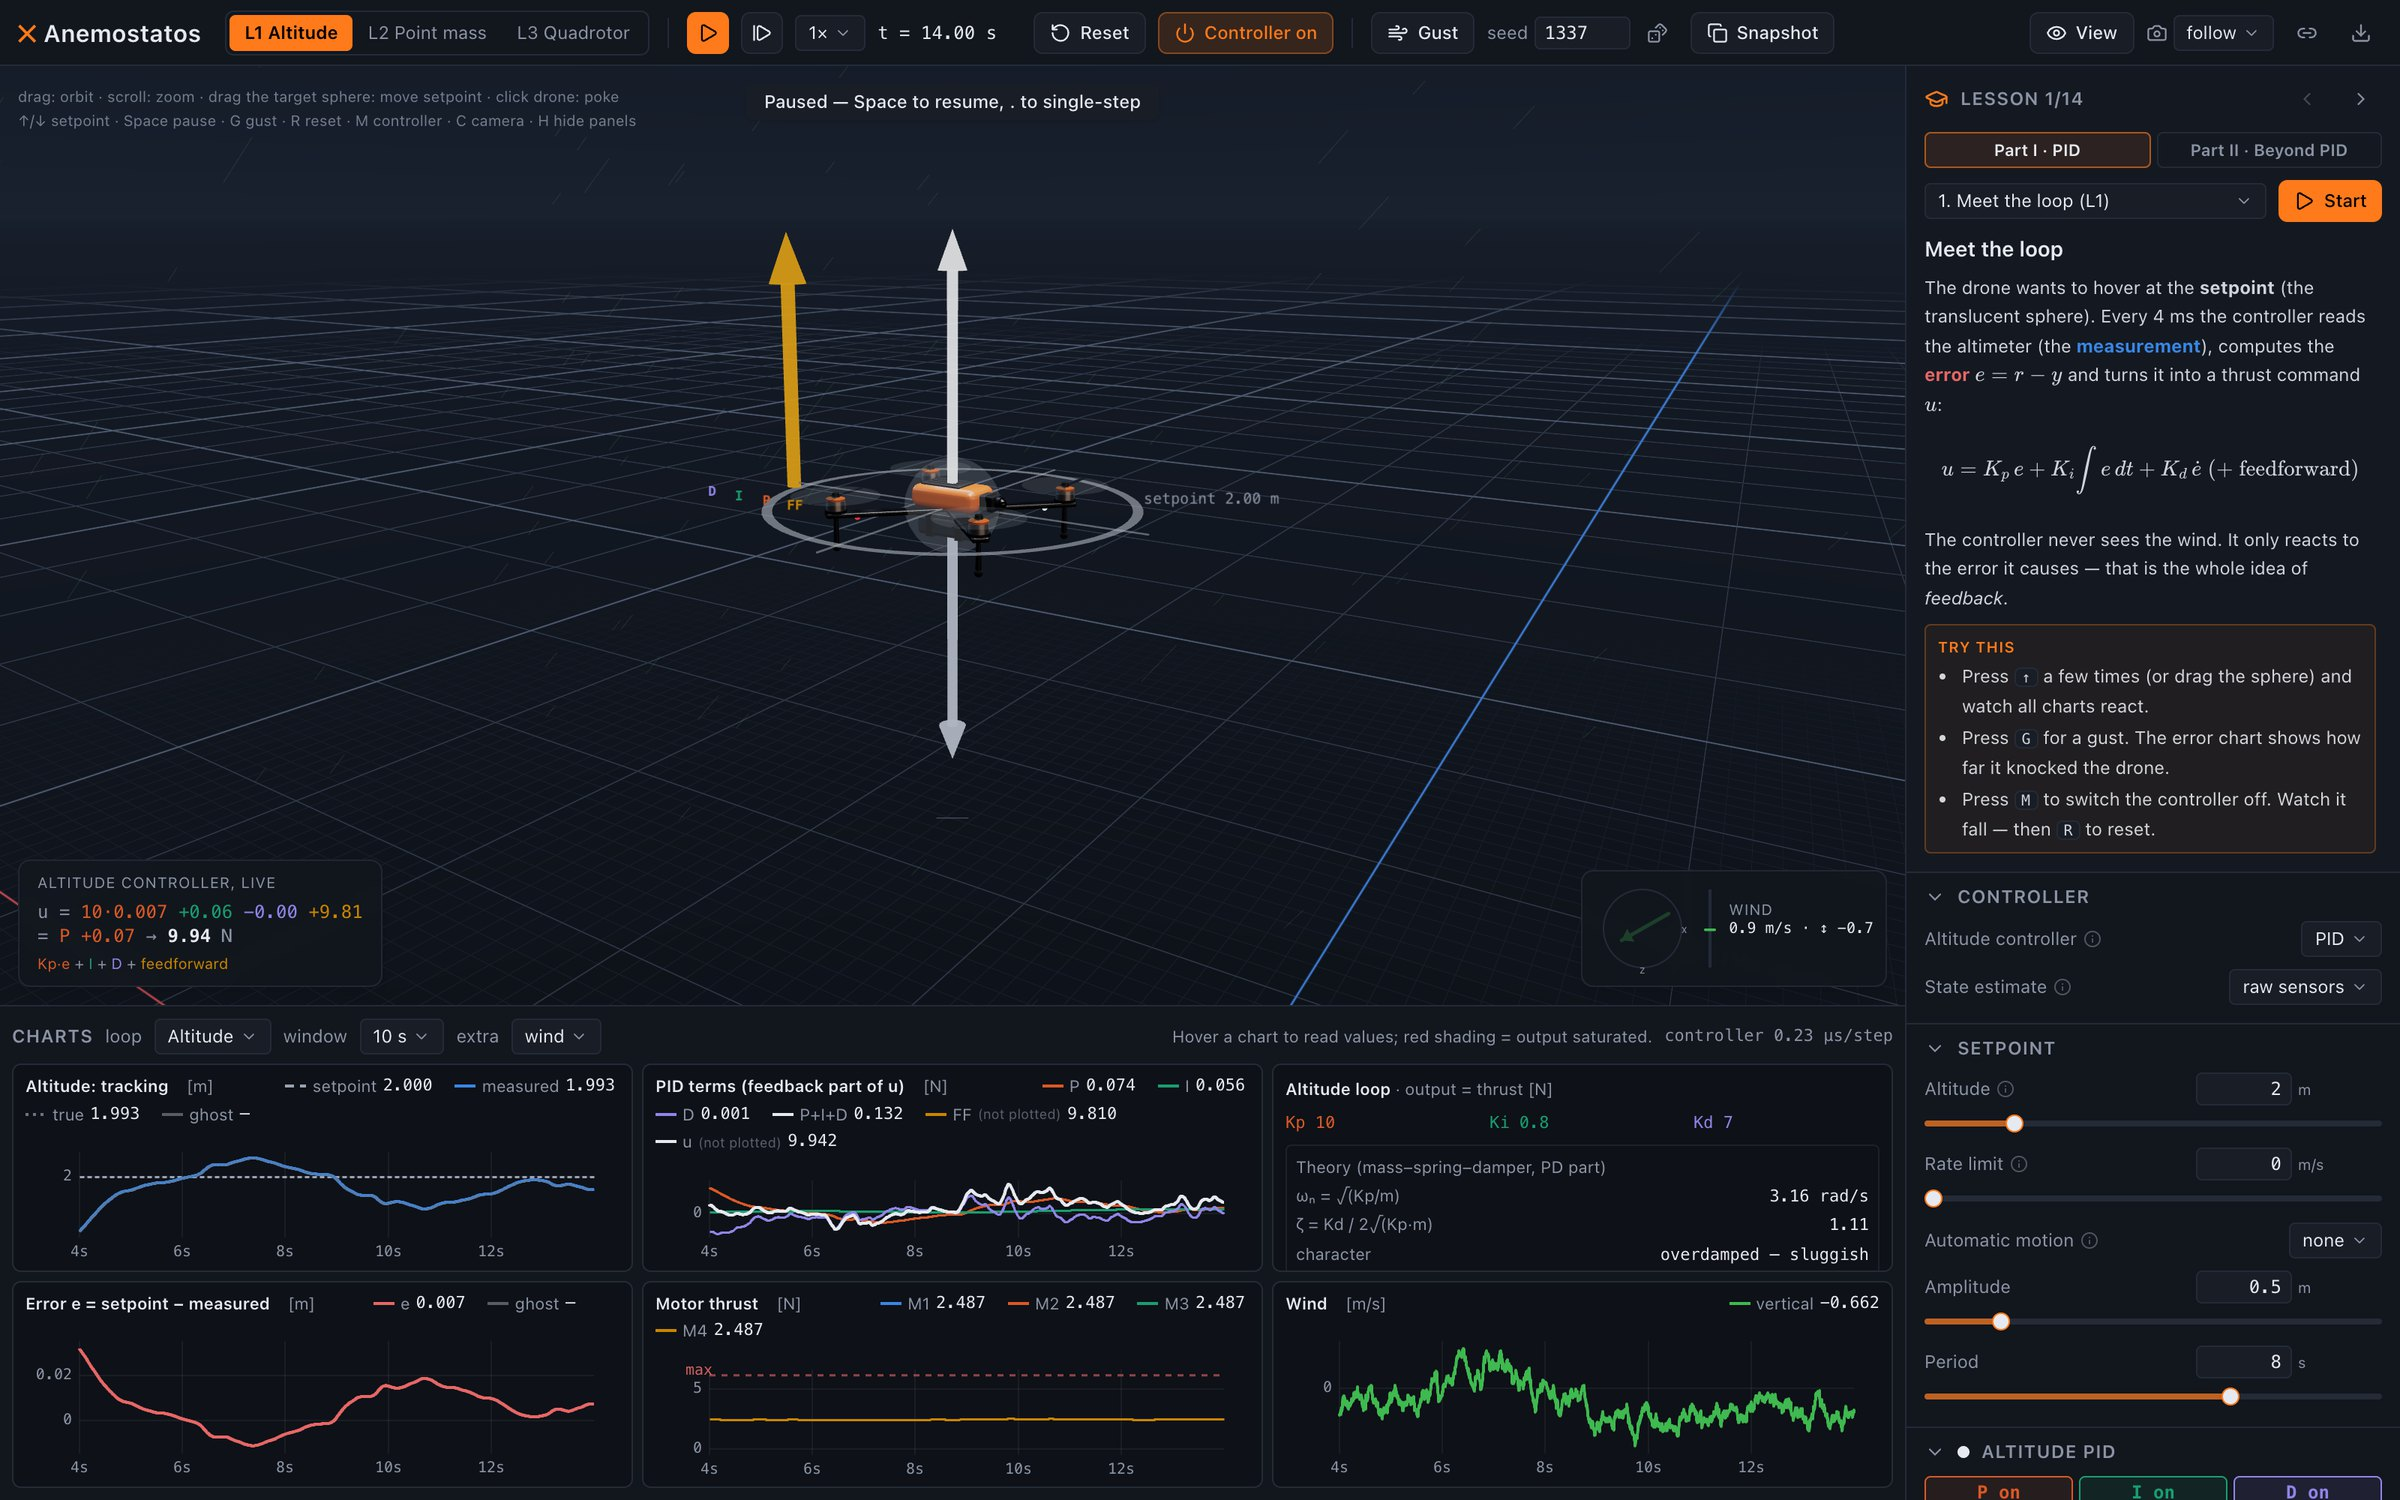
\includegraphics[width=\linewidth]{screens/meet}};
      \begin{scope}[x={(img.south east)}, y={(img.north west)}]
        \node[mk] at (0.183,0.940) {1};
        \node[mk] at (0.300,0.940) {2};
        \node[mk] at (0.584,0.940) {3};
        \node[mk] at (0.735,0.940) {4};
        \node[mk] at (0.900,0.945) {5};
        \node[mk] at (0.285,0.910) {6};
        \node[mk] at (0.493,0.890) {7};
        \node[mk] at (0.545,0.700) {8};
        \node[mk] at (0.168,0.392) {9};
        \node[mk] at (0.648,0.392) {10};
        \node[mk] at (0.806,0.934) {11};
        \node[mk] at (0.784,0.402) {12};
        \node[mk] at (0.256,0.312) {13};
        \node[mk] at (0.030,0.270) {a};
        \node[mk] at (0.292,0.270) {b};
        \node[mk] at (0.554,0.270) {c};
        \node[mk] at (0.030,0.125) {d};
        \node[mk] at (0.292,0.125) {e};
        \node[mk] at (0.554,0.125) {f};
      \end{scope}
    \end{tikzpicture}
    \caption{The screen of Anemostatos, its parts numbered as in \cref{tab:map-screen}. The screen is a grid: the toolbar across the top, the 3D view, the side panel on the right (lessons above, parameters below) and the six charts underneath. \key{H} hides the side panel and the charts and leaves the 3D view alone.}
    \label{fig:map-screen}
  \end{fullwidth}
\end{figure}

\Cref{fig:map-screen} is the screen during Lesson~I.1, and \cref{tab:map-screen} names its parts. The layout itself is in \src{src/App.tsx}: a toolbar \SI{44}{px} high, a side panel \SI{330}{px} wide and a chart area \SI{330}{px} high around the 3D view.

\begin{table}[tbp]
\begin{fullwidth}\footnotesize\let\ui\uitab
\renewcommand{\arraystretch}{1.22}
\begin{tabularx}{\linewidth}{@{}>{\sffamily\bfseries\color{accent}}l>{\raggedright}p{36mm}>{\raggedright\arraybackslash}X>{\raggedright\arraybackslash}p{37mm}@{}}
\toprule
 & \normalfont\sffamily part & \sffamily what it does & \sffamily source\\
\midrule
1 & \ui{L1 Altitude · L2 Point mass · L3 Quadrotor} & The level (\cref{tab:map-levels}). Changing it restarts the run. Keys \key{1} \key{2} \key{3}. & \tsrc{ui/Toolbar.tsx}\\
2 & pause, single step, speed, clock & Pause or resume (\key{Space}); one controller period forward while paused (\key{.}); simulation speed $0.1\times$ to $4\times$; the simulated time $t$. & \tsrc{ui/Toolbar.tsx}\\
 & \ui{Reset}, \ui{Controller on} & Restart from the ground with the current parameters (\key{R}); switch the controller off, motors idle, and on again (\key{M}). & \tsrc{engine/simulation.ts}\\
3 & \ui{Gust}, \ui{seed} & A strong gust now (\key{G}). The seed of the wind: same seed and same parameters, the same wind to the millisecond; the dice draw a new one. & \tsrc{ui/actions.ts}, \tsrc{sim/wind.ts}\\
4 & \ui{Snapshot} & Freeze the run as a grey \emph{ghost} trace in the charts (\key{S}); change something, press \key{R}, compare on the same wind. A chip \ui{ghost: …} beside it removes the ghost. & \tsrc{ui/actions.ts}\\
5 & \ui{View}, camera & \ui{View}: the 3D overlays \ui{Forces}, \ui{P / I / D arrows}, \ui{Setpoint marker}, \ui{Height ruler}, \ui{Trail}, \ui{Wind tracers}. The camera: \ui{orbit}, \ui{follow} (the default), \ui{side}, \ui{top}; \key{C} cycles. Then: copy a link with every parameter; download the last \SI{60}{s} of telemetry as CSV. & \tsrc{ui/Toolbar.tsx}, \tsrc{scene/CameraRig.tsx}\\
6 & hint line & The mouse and the keys, in one line. & \tsrc{App.tsx}\\
7 & status badges & \ui{Crashed!}, \ui{Controller off}, \ui{Taking off…} (integrators held until airborne), \ui{Paused}, \ui{Simulation slowed down}. & \tsrc{ui/hud/StatusBadges.tsx}\\
8 & 3D view & The drone, the translucent setpoint sphere (drag it), the force arrows in the colours of the terms, the wind tracers. & \tsrc{scene/Scene.tsx}\\
9 & live formula & The controller's output as the sum of its terms, with this instant's numbers; for a controller other than PID, the sum of its named contributions. & \tsrc{ui/hud/LiveFormula.tsx}\\
10 & wind indicator & Direction and speed of the wind at the drone, and its vertical part. & \tsrc{ui/hud/WindHud.tsx}\\
11 & lesson panel & Parts I–IV, the lesson list with its level, \ui{Start}, the text and its \emph{Try this}, and the \ui{Goal}, which turns green when reached. Arrows step through the lessons. & \tsrc{lessons/LessonPanel.tsx}\\
12 & parameter panel & Every parameter, in collapsible groups (\cref{tab:map-groups}). & \tsrc{ui/params/ParamPanel.tsx}\\
13 & chart header & \ui{loop}, \ui{window} (\SIlist{5;10;30;60}{s}), \ui{extra}, \ui{beside it}, and the time the controller takes per step. & \tsrc{ui/charts/ChartsPanel.tsx}\\
a–f & the six charts & See \cref{tab:map-charts}. & \tsrc{ui/charts/}\\
\bottomrule
\end{tabularx}
\caption{The parts of the screen, as numbered in \cref{fig:map-screen}.}
\label{tab:map-screen}
\end{fullwidth}
\end{table}

\subsection*{The parameter panel}

Each group of the panel (\cref{tab:map-groups}) folds open with a click on its title; \ui{Controller}, \ui{Setpoint}, \ui{Altitude PID}, \ui{LQR}, \ui{ADRC} and \ui{Kalman filter} start open, and so does \ui{Horizontal PID (X, Z)} above Level~1. A group appears only when it applies: the PID groups when a PID flies, \ui{MPC} when MPC is chosen, a field such as \ui{X} only on the levels that have it, and a choice with a single option not at all. Every number has a slider and a box for typing; the small arrow beside the box returns it to its default, and the \textsf{i} beside a label explains the parameter. In a PID group three coloured buttons, \ui{P on · I on · D on}, switch the terms, and the less common settings, \ui{D acts on}, \ui{D filter}, \ui{Anti-windup}, \ui{I limit} and \ui{Kb}, wait under \ui{Practical details (D filter, anti-windup…)}. Clicking the title of a group that belongs to a loop shows that loop in the charts.

\subsection*{The charts}

The chart area is a grid of three columns and two rows (\cref{tab:map-charts}). The \ui{loop} menu chooses which control loop the four left charts and the card show; \cref{tab:map-levels} lists the loops of each level. Hovering a chart reads its values; a red band means the output of the loop was saturated.

\begin{table}[tbp]
\begin{fullwidth}\footnotesize\let\ui\uitab
\renewcommand{\arraystretch}{1.22}
\begin{tabularx}{\linewidth}{@{}>{\sffamily\bfseries\color{accent}}l>{\raggedright}p{40mm}>{\raggedright\arraybackslash}X@{}}
\toprule
 & \normalfont\sffamily chart & \sffamily what it shows\\
\midrule
a & \ui{\emph{loop}: tracking} & The setpoint (dashed), the measurement, the true value when the sensor lies, and the ghost.\\
b & \ui{PID terms (feedback part of u)} & \Pt, \It, \Dt\ and their sum, with the feedforward and the total $u$ in the legend; for any other controller, \ui{Contributions}.\\
c & info card & The gains, and for the force loops of L1 and L2 the theory of the PD part: $\omega_n$, $\zeta$, the character of the response, the predicted steady-state error, $T_i$ and $T_d$. Below, the step metrics of the last setpoint step: rise time 10–90\,\%, overshoot, settling time $\pm 2\,\%$, steady-state error. A controller other than PID lists what it says about itself (gains, poles, estimates); at L3 a planned trajectory shows the speed, acceleration and tilt it needs (\tsrc{ui/charts/InfoCard.tsx}, \tsrc{ui/charts/StepMetrics.tsx}).\\
d & \ui{Error e = setpoint − measured} & The error of the loop, and the ghost's.\\
e & \ui{Motor thrust} & The four motors, with their maximum. The menu \ui{beside it} replaces it with \ui{Bode plot}, \ui{Nyquist plot}, \ui{pole map} or \ui{filter uncertainty}.\\
f & \ui{extra}: \ui{wind} & The default. Part II uses \ui{disturbance} (the force the model does not explain, true and estimated), \ui{phase portrait} and \ui{estimate vs truth}; the later parts add the analysis charts. A tall chart, such as the Bode plot, takes the whole right column in place of c and f.\\
\bottomrule
\end{tabularx}
\caption{The six charts, lettered as in \cref{fig:map-screen}: top row a, b, c; bottom row d, e, f.}
\label{tab:map-charts}
\end{fullwidth}
\end{table}

\section*{Keys and mouse}

The keys are read in \src{src/ui/useKeyboard.ts} and act anywhere except while typing in a box. The mouse acts on the 3D view: the drone in \src{src/scene/DroneRig.tsx}, the setpoint sphere in \src{src/scene/overlays/SetpointGhost.tsx}.

\begin{center}\small
\renewcommand{\arraystretch}{1.25}
\begin{tabularx}{\linewidth}{@{}>{\raggedright}p{27mm}>{\raggedright\arraybackslash}X@{}}
\toprule
\sffamily key & \sffamily action\\
\midrule
\key{Space} & pause and resume\\
\key{.} & one controller period forward, while paused\\
\key{R} & reset: restart from the ground; a lesson's scripted events replay\\
\key{M} & controller on and off\\
\key{G} & a strong gust now\\
\key{↑}\ \key{↓} & altitude setpoint up or down by \SI{0.1}{m}; with \key{Shift}, by \SI{1}{m} (kept within \SIrange{0.2}{10}{m})\\
\key{1}\ \key{2}\ \key{3} & Level~1, 2 or 3\\
\key{C} & next camera: orbit, follow, side, top\\
\key{S} & snapshot: keep this run as the ghost\\
\key{H} & hide or show the side panel and the charts\\
\midrule
\sffamily mouse & \\
\midrule
drag, scroll & orbit the camera, zoom\\
drag the sphere & move the setpoint: vertically at L1; horizontally at L2 and L3, vertically with \key{Shift}\\
click the drone & a shove: downwards at L1, away from the camera at L2 and L3\\
\bottomrule
\end{tabularx}
\end{center}

\section*{The three levels}

The same drone is simulated at three levels of truth (\cref{tab:map-levels}). The physics always runs at \SI{1}{kHz} (\src{src/engine/simulation.ts}); the controller runs at \ui{Controller rate}, \param{control.rateHz}, \SI{250}{Hz} by default. \param{sim.level} holds the level, and a link made with the toolbar keeps it.

\begin{table}[tbp]
\begin{fullwidth}\footnotesize\let\ui\uitab
\renewcommand{\arraystretch}{1.22}
\begin{tabularx}{\linewidth}{@{}>{\sffamily\bfseries\color{accent}}l>{\raggedright}X>{\raggedright}p{43mm}>{\raggedright\arraybackslash}p{46mm}@{}}
\toprule
 & \normalfont\sffamily the vehicle & \sffamily loops in the charts & \sffamily controllers\\
\midrule
L1 & \textbf{Altitude.} The drone moves only up and down; the four motors push together, the controller chooses the total thrust. & \ui{Altitude} (\texttt{alt}) & \tsrc{control/registry.ts}: one of eleven altitude controllers (\cref{tab:map-controllers}), with or without a Kalman filter\\
L2 & \textbf{Point mass.} Three independent forces push a point in 3D. A cheat: a real drone must tilt. & \ui{Position X, Y, Z} (\texttt{pos.x}, \texttt{pos.y}, \texttt{pos.z}); default \texttt{pos.y} & \tsrc{control/pointmass.ts}: \ui{Altitude PID} on Y, \ui{Horizontal PID (X, Z)} on X and Z\\
L3 & \textbf{Quadrotor.} Six degrees of freedom: four motors with lag, attitude as a quaternion, the cascade position → velocity → attitude → rate → motors. & \ui{Position}, \ui{Velocity}, \ui{Attitude} and \ui{Rate} on each axis (\texttt{pos.x} … \texttt{rate.yaw}), \ui{Accel} with acceleration INDI; default \texttt{pos.y} & \tsrc{control/cascade.ts}, built from the five choices of \cref{tab:map-controllers3}\\
\bottomrule
\end{tabularx}
\caption{The levels. The physics of all three is in \tsrc{sim/dynamics.ts}, the wind in \tsrc{sim/wind.ts} and the sensors in \tsrc{sim/sensors.ts}; the loops are listed in \tsrc{ui/charts/loops.ts}.}
\label{tab:map-levels}
\end{fullwidth}
\end{table}

\section*{The controllers}

What flies is chosen in the group \ui{Controller}, and \src{src/control/registry.ts} builds it; any change of choice restarts the run. \Cref{tab:map-controllers,tab:map-controllers3} list every option by its label on the screen, its value in the parameters and the file that implements it. At L2 there is nothing to choose, and the group is hidden.

\begin{table}[tbp]
\begin{fullwidth}\footnotesize\let\ui\uitab
\renewcommand{\arraystretch}{1.13}
\begin{tabularx}{\linewidth}{@{}>{\raggedright}p{43mm}>{\raggedright}p{27mm}>{\raggedright}X>{\raggedright\arraybackslash}p{25mm}@{}}
\toprule
\sffamily option on the screen & \sffamily value & \sffamily source & \sffamily lessons\\
\midrule
\multicolumn{4}{@{}l}{\sanscaps\scriptsize\color{accent}L1 · ALTITUDE CONTROLLER\quad\normalfont\param{control.l1.kind}}\\
\ui{PID} (default) & \texttt{pid} & \tsrc{control/altitude.ts}, \tsrc{control/pid.ts} & Part I, II.1\\
\ui{LQR / LQI} & \texttt{lqr} & \tsrc{control/lqr.ts} & II.2, II.3\\
\ui{ADRC} & \texttt{adrc} & \tsrc{control/adrc.ts}, \tsrc{estimation/eso.ts} & II.5, II.6\\
\ui{MPC} & \texttt{mpc} & \tsrc{control/mpc.ts}, \tsrc{math/qp.ts} & II.13, II.14\\
\ui{L1 adaptive} & \texttt{l1ac} & \tsrc{control/l1ac.ts} & II.18\\
\ui{H∞ loop shaping}, \ui{sliding mode}, \ui{MRAC (adaptive)}, \ui{backstepping} & \texttt{hinf}, \texttt{smc}, \texttt{mrac}, \texttt{backstepping} & \tsrc{control/hinf.ts}, \tsrc{control/smc.ts}, \tsrc{control/mrac.ts}, \tsrc{control/backstepping.ts} & Part III\\
\ui{bang-bang (time-optimal)}, \ui{dynamic programming} & \texttt{bangbang}, \texttt{dp} & \tsrc{control/bangbang.ts}, \tsrc{control/dp.ts} & Part IV\\
\multicolumn{4}{@{}l}{\sanscaps\scriptsize\color{accent}L1 · STATE ESTIMATE\quad\normalfont\param{control.l1.estimator}}\\
\ui{raw sensors} (default), \ui{Kalman filter} & \texttt{none}, \texttt{kalman} & \tsrc{control/estimated.ts}, \tsrc{estimation/kalman.ts} & II.4\\
\bottomrule
\end{tabularx}
\caption{The controllers of Level~1, chosen in the group \ui{Controller}.}
\label{tab:map-controllers}
\end{fullwidth}
\end{table}

\begin{table}[tbp]
\begin{fullwidth}\footnotesize\let\ui\uitab
\renewcommand{\arraystretch}{1.13}
\begin{tabularx}{\linewidth}{@{}>{\raggedright}p{43mm}>{\raggedright}p{27mm}>{\raggedright}X>{\raggedright\arraybackslash}p{25mm}@{}}
\toprule
\sffamily option on the screen & \sffamily value & \sffamily source & \sffamily lessons\\
\midrule
\multicolumn{4}{@{}l}{\sanscaps\scriptsize\color{accent}L3 · OUTER STAGE\quad\normalfont\param{control.l3.outer}}\\
\ui{PID cascade} (default) & \texttt{pid-cascade} & \tsrc{control/cascade.ts}, \tsrc{control/pid.ts} & I.13, I.14\\
\ui{geometric tracking (Lee)} & \texttt{geometric} & \tsrc{control/geometric.ts} & II.10–II.12\\
\ui{MPC (linear, point mass)} & \texttt{mpc} & \tsrc{control/mpc.ts} & II.15\\
\ui{MPPI (sampling)} & \texttt{mppi} & \tsrc{control/mppi.ts} & II.16\\
\ui{neural network policy} & \texttt{policy} & \tsrc{control/policy.ts}, \tsrc{control/policy-weights.ts} & II.20\\
\multicolumn{4}{@{}l}{\sanscaps\scriptsize\color{accent}L3 · ATTITUDE LAW\quad\normalfont\param{control.l3.attitude}}\\
\ui{quaternion error} (default), \ui{tilt-prioritised}, \ui{Euler angles (naive)} & \texttt{quaternion}, \texttt{tilt}, \texttt{euler} & \tsrc{control/geometric.ts}, \tsrc{math/quat.ts} & II.10\\
\multicolumn{4}{@{}l}{\sanscaps\scriptsize\color{accent}L3 · INNER STAGE\quad\normalfont\param{control.l3.inner}}\\
\ui{attitude P + rate PID} (default) & \texttt{pid} & \tsrc{control/stages.ts} (\texttt{PidRateStage}) & I.13\\
\ui{attitude P + rate INDI} & \texttt{indi} & \tsrc{control/stages.ts} (\texttt{RateIndi}) & II.7, II.9\\
\multicolumn{4}{@{}l}{\sanscaps\scriptsize\color{accent}L3 · DISTURBANCE COMPENSATION\quad\normalfont\param{control.l3.compensation}}\\
\ui{none (m̂·a model)} (default) & \texttt{none} & \tsrc{control/stages.ts} (\texttt{NoCompensation}) & \\
\ui{acceleration INDI} & \texttt{indi} & \tsrc{control/stages.ts} (\texttt{AccelIndi}) & II.8, II.15\\
\ui{L1 adaptive} & \texttt{l1ac} & \tsrc{control/l1ac.ts} (\texttt{L1Compensation}) & II.18\\
\ui{learned residual model} & \texttt{learned} & \tsrc{control/residual.ts} & II.19\\
\multicolumn{4}{@{}l}{\sanscaps\scriptsize\color{accent}L3 · SAFETY FILTER\quad\normalfont\param{control.l3.safety}}\\
\ui{none} (default), \ui{control barrier function} & \texttt{none}, \texttt{cbf} & \tsrc{control/cbf.ts} & II.17\\
\bottomrule
\end{tabularx}
\caption{The controllers of Level~3. The rotor-loss controller of Part III, \tsrc{control/fault.ts}, replaces the PID cascade when \param{control.fault.enabled} is set.}
\label{tab:map-controllers3}
\end{fullwidth}
\end{table}

\section*{The parameter groups}

\Cref{tab:map-groups,tab:map-groups2} list the groups that Parts I and II use, in the order of the panel. A path ending in \texttt{.*} stands for a whole PID: \texttt{kp}, \texttt{ki}, \texttt{kd}, the switches \texttt{pOn}, \texttt{iOn}, \texttt{dOn}, and the practical details \texttt{derivativeOn}, \texttt{dFilterHz}, \texttt{antiWindup}, \texttt{iLimit}, \texttt{kb} (\src{src/control/pid.ts}). The defaults of every parameter are in \texttt{defaultParams} of \src{src/sim/params.ts}.

The groups of the later parts follow in the panel: \ui{Loop shaping}, the groups of the Part~III controllers, \ui{Uncertainty (plant family)}, \ui{Rotor loss}, \ui{Fault monitor}, \ui{Vibration \& IMU}, \ui{Attitude estimate}, \ui{Guidance (chase a target)}, \ui{Inertial navigation \& beacons}, \ui{Navigation}, \ui{Gyro filter}, \ui{Identification (chirp)} and \ui{Probe (frequency response)}, and, when \ui{Physics\then Vehicle} is not the quadrotor, the groups of the rocket, the aircraft and the satellite of Part~IV.

\begin{table}[p]
\begin{fullwidth}\footnotesize\let\ui\uitab
\renewcommand{\arraystretch}{1.12}
\begin{tabularx}{\linewidth}{@{}>{\raggedright}p{30mm}>{\raggedright}X>{\raggedright}p{33mm}>{\raggedright\arraybackslash}p{21mm}@{}}
\toprule
\sffamily group & \sffamily parameters & \sffamily shown & \sffamily lessons\\
\midrule
\ui{Controller} & \param{control.l1.kind}, \param{control.l1.estimator}; \param{control.l3.outer}, \param{.attitude}, \param{.inner}, \param{.compensation}, \param{.safety} & L1 and L3 & II.2–II.20\\
\ui{Setpoint} & \param{setpoint.y}, \param{.x}, \param{.z} (L2, L3), \param{.yawDeg} (L3), \param{.rateLimit}; \ui{Automatic motion}: \param{.profile}, \param{.profileAxis}, \param{.profileAmplitude}, \param{.profilePeriod} & always & I.4, I.7, II.11, II.12\\
\ui{Altitude PID} & \param{control.alt.*}; \param{control.feedforward}, \param{control.model.mass}, \param{control.rateHz} & L1 with PID; L2 & I.1–I.11\\
\ui{LQR} & \param{control.lqr.qPos}, \param{.qVel}, \param{.r}, \param{.integral}, \param{.qInt}, \param{.lagState}, \param{.observer}, \param{.kfQ}, \param{.kfR}; \param{control.model.motorTau} & L1, \ui{LQR / LQI} & II.2, II.3\\
\ui{ADRC} & \param{control.adrc.wc}, \param{.wo} & L1, \ui{ADRC} & II.5, II.6\\
\ui{Kalman filter} & \param{control.kalman.accSigma}, \param{.posSigma}, \param{.biasSigma}, \param{.altBiasState}, \param{.altBiasSigma} & L1, \ui{State estimate} Kalman & II.4\\
\ui{Horizontal PID (X, Z)} & \param{control.posH.*}, \param{control.maxHForce} & L2 & I.12\\
\ui{Geometric tracking} & \param{control.geometric.kp}, \param{.kv}, \param{.ki}, \param{.feedforward} & L3, geometric outer stage & II.10–II.12\\
\ui{Position P} & \param{control.l3.posKpH}, \param{.posKpV}, \param{.vMaxH}, \param{.vMaxV}, \param{.hzPos} & L3, PID cascade & I.13, I.14\\
\ui{Velocity PID — horizontal} & \param{control.l3.velH.*}, \param{control.l3.maxTiltDeg}, \param{.hzVel} & L3, PID cascade & I.13\\
\ui{Velocity PID — vertical} & \param{control.l3.velV.*}, \param{control.feedforward}, \param{control.model.mass} & L3, PID cascade & I.13\\
\ui{Attitude P} & \param{control.l3.attKpRP}, \param{.attKpYaw}, \param{.maxRateDeg}, \param{.hzAtt} & L3 & I.13, I.14\\
\ui{Rate PID — roll/pitch}, \ui{Rate PID — yaw} & \param{control.l3.rateRP.*}, \param{control.l3.rateYaw.*}, \param{control.l3.hzRate}, \param{control.model.imuYawDeg} & L3, rate PID & I.13, II.7\\
\bottomrule
\end{tabularx}
\caption{The parameter groups of the controllers used in Parts I and II (\tsrc{engine/schema.ts}). A path that begins with a dot continues the one before it. \enquote{Shown} is when the group appears; a level in brackets after a field restricts that field.}
\label{tab:map-groups}
\end{fullwidth}
\end{table}

\begin{table}[p]
\begin{fullwidth}\footnotesize\let\ui\uitab
\renewcommand{\arraystretch}{1.12}
\begin{tabularx}{\linewidth}{@{}>{\raggedright}p{30mm}>{\raggedright}X>{\raggedright}p{33mm}>{\raggedright\arraybackslash}p{21mm}@{}}
\toprule
\sffamily group & \sffamily parameters & \sffamily shown & \sffamily lessons\\
\midrule
\ui{Physics} & \param{drone.mass}, \param{.maxMotorThrust}, \param{.motorTau}, \param{.dragV}, \param{.dragH} (L2, L3); \param{sim.vehicle} (L1) & always & I.5, I.6, I.9\\
\ui{Wind} & \param{wind.enabled}, \param{.meanSpeed} and \param{.meanHeading} (L2, L3), \param{.meanVertical}, \param{.turbSigma}, \param{.turbTau}, \param{.gustsOn}, \param{.gustsPerMinute}, \param{.gustAmpMin}, \param{.gustAmpMax}, \param{.gustDurMin}, \param{.gustDurMax}, \param{.gustVertical} & always & I.11–I.13, II.8\\
\ui{INDI} & \param{control.indi.rateKpRP}, \param{.rateKpYaw}, \param{.filterHz}, \param{.accFilterHz}, \param{.syncFilters}; \param{control.model.inertiaScale}, \param{.motorTau} & L3, INDI inner stage or compensation & II.7–II.9, II.15\\
\ui{L1 adaptive} & \param{control.l1ac.filterHz}, \param{.as}, \param{.wc} & L1, or L3 compensation & II.18\\
\ui{Learned residual model} & \param{control.residual.forgetting}, \param{.filterHz} & L3, learned compensation & II.19\\
\ui{Keep-out zones} & \param{world.ceiling}; \param{world.pillar}, \param{.pillarX}, \param{.pillarZ}, \param{.pillarR} (L2, L3) & always & II.13, II.14, II.16, II.17\\
\ui{MPC} & \param{control.mpc.horizon}, \param{.hz}, \param{.qPos}, \param{.qVel}, \param{.r}, \param{.iterations}, \param{.margin} & L1 MPC, or L3 MPC outer stage & II.13–II.15\\
\ui{MPPI} & \param{control.mppi.samples}, \param{.lambda}, \param{.sigma}, \param{.horizon}, \param{.qPos}, \param{.zoneWeight}, \param{.margin} & L3, MPPI outer stage & II.16\\
\ui{Safety filter (CBF)} & \param{control.cbf.gamma}, \param{.margin} & L3, CBF & II.17\\
\ui{Faults \& aerodynamics} & \param{drone.motorEfficiency.0}–\param{3} (L1, L3), \param{drone.rotorDrag} (L3), \param{drone.motorSlew} & always & II.7, II.19\\
\ui{Sensors} & \param{sensors.posNoise}, \param{.velNoise} (L1, L3), \param{.gyroNoise} (L3), \param{.altBias}, \param{.delayMs}, \param{.posRateHz}, \param{.accNoise}, \param{.accBias} (L1, L3), \param{.motorFeedback} (L1, L3), and the faults of Part III & always & I.8, I.9, II.4, II.6, II.9\\
\bottomrule
\end{tabularx}
\caption{The parameter groups of the vehicle, its world and its sensors, continuing \cref{tab:map-groups}.}
\label{tab:map-groups2}
\end{fullwidth}
\end{table}

\clearpage
\section*{The lessons, one by one}

\Cref{tab:map-part1,tab:map-part2} give, for every lesson of Parts I and II, its id in the app (the one printed on the lesson's opening page), its level, what \ui{Start} changes from the defaults, and the files that the lesson is about. Everything not named stays at its default: at L1 a PID with gravity feedforward, $K_p = 10$, $K_i = 0.8$, $K_d = 7$, at \SI{250}{Hz}, setpoint \SI{2}{m}, wind with turbulence and gusts, seed 1337. \enquote{Calm} means \param{wind.enabled} off; \enquote{steps} is the setpoint profile \ui{square wave (steps)}, given by amplitude and period; \enquote{ghost} is a comparison run flown when the lesson starts. The set-ups are in \src{src/lessons/lessons.tsx} (Part I) and \src{src/lessons/part2.tsx} (Part II).

\begin{table}[tbp]
\begin{fullwidth}\footnotesize\let\ui\uitab
\renewcommand{\arraystretch}{1.16}
\begin{tabularx}{\linewidth}{@{}>{\sffamily\color{accent}}l>{\raggedright}p{27mm}>{\ttfamily\footnotesize}l>{\sffamily}l>{\raggedright}X>{\raggedright\arraybackslash}p{35mm}@{}}
\toprule
 & \sffamily lesson & \normalfont\sffamily\small id & & \sffamily what \ui{Start} sets & \sffamily main sources\\
\midrule
I.1 & \hyperref[les:meet]{Meet the loop} & meet & L1 & the defaults & \tsrc{control/altitude.ts}, \tsrc{control/pid.ts}, \tsrc{sim/dynamics.ts}\\
I.2 & \hyperref[les:spring]{Just a spring} & spring & L1 & calm; I and D off; setpoint to \SI{3}{m} at \SI{6}{s} & \tsrc{control/pid.ts}, \tsrc{ui/charts/InfoCard.tsx}\\
I.3 & \hyperref[les:droop]{The gravity droop} & droop & L1 & calm; gravity feedforward off; I off & \tsrc{control/altitude.ts}, \tsrc{ui/charts/InfoCard.tsx}\\
I.4 & \hyperref[les:damper]{Add a damper} & damper & L1 & calm; I off, $K_d = 0.8$; steps \SI{0.5}{m}, \SI{8}{s}. Goal: overshoot below 2\,\%, settling below \SI{2.5}{s} & \tsrc{engine/metrics.ts}, \tsrc{ui/charts/StepMetrics.tsx}\\
I.5 & \hyperref[les:integral]{Integral to the rescue} & integral & L1 & calm; true mass \SI{1.4}{kg}; I off. Goal: steady-state error below \SI{1}{cm} & \tsrc{control/pid.ts}\\
I.6 & \hyperref[les:windup]{Windup} & windup & L1 & calm; \SI{3}{N} per motor; $K_i = 3$, anti-windup none; setpoint to \SI{6}{m} at \SI{8}{s} & \tsrc{control/pid.ts}\\
I.7 & \hyperref[les:kick]{Derivative kick} & kick & L1 & calm; D on the error, no D filter; steps \SI{0.5}{m}, \SI{6}{s} & \tsrc{control/pid.ts}\\
I.8 & \hyperref[les:noise]{Noisy sensor} & noise & L1 & calm; position noise \SI{1}{cm}; no D filter & \tsrc{control/pid.ts}, \tsrc{sim/sensors.ts}\\
I.9 & \hyperref[les:slow]{Too slow to react} & slow & L1 & calm; steps \SI{0.5}{m}, \SI{8}{s} & \tsrc{engine/simulation.ts}, \tsrc{sim/sensors.ts}\\
I.10 & \hyperref[les:edge]{Find the edge} & edge & L1 & calm; I off; steps \SI{0.3}{m}, \SI{6}{s} & \tsrc{sim/dynamics.ts}\\
I.11 & \hyperref[les:challenge]{Gust challenge} & challenge & L1 & seed 4242; 14 gusts a minute of 4--\SI{10}{m/s}; turbulence \SI{1.2}{m/s}. Goal: a lower RMS error from 5 to \SI{65}{s} than the default tune & \tsrc{sim/wind.ts}, \tsrc{lessons/lessons.tsx}\\
I.12 & \hyperref[les:tilt]{Why drones tilt} & tilt & L2 & mean wind \SI{4}{m/s}, gusts 20\,\% vertical; loop \texttt{pos.x} & \tsrc{control/pointmass.ts}\\
I.13 & \hyperref[les:cascade]{The cascade} & cascade & L3 & mean wind \SI{5}{m/s}, no gusts, turbulence \SI{0.3}{m/s}; loop \texttt{vel.x} & \tsrc{control/cascade.ts}, \tsrc{control/stages.ts}, \tsrc{control/mixer.ts}\\
I.14 & \hyperref[les:inversion]{Cascade inversion} & inversion & L3 & calm; steps on X, \SI{1.5}{m}, \SI{8}{s}; loop \texttt{att.pitch} & \tsrc{control/cascade.ts}\\
\bottomrule
\end{tabularx}
\caption{The lessons of Part I.}
\label{tab:map-part1}
\end{fullwidth}
\end{table}

\begin{table}[p]
\begin{fullwidth}\footnotesize\let\ui\uitab
\renewcommand{\arraystretch}{1.04}
\begin{tabularx}{\linewidth}{@{}>{\sffamily\color{accent}}l>{\raggedright}p{27mm}>{\ttfamily\footnotesize}l>{\sffamily}l>{\raggedright}X>{\raggedright\arraybackslash}p{35mm}@{}}
\toprule
 & \sffamily lesson & \normalfont\sffamily\small id & & \sffamily what \ui{Start} sets & \sffamily main sources\\
\midrule
\multicolumn{6}{@{}l}{\sanscaps\scriptsize\color{accent}A · FROM KNOBS TO MODELS}\\
II.1 & \hyperref[les:state]{State, not error} & state & L1 & calm; steps \SI{0.5}{m}, \SI{8}{s}; $K_d = 6.3$, I off; extra: phase portrait & \tsrc{ui/charts/PhasePortrait.tsx}\\
II.2 & \hyperref[les:lqr]{Pay for what you want} & lqr & L1 & calm; steps; LQR with $r = 10$; ghost: PD & \tsrc{control/lqr.ts}, \tsrc{math/riccati.ts}\\
II.3 & \hyperref[les:lqi]{Integral, the optimal way} & lqi & L1 & calm; LQR, assumed mass \SI{0.8}{kg}; setpoint to \SI{3}{m} at \SI{15}{s} & \tsrc{control/lqr.ts}\\
II.4 & \hyperref[les:kalman]{Trust issues} & kalman & L1 & calm; position noise \SI{5}{cm} at \SI{50}{Hz}, accelerometer noise \SI{0.3}{m/s^2} and bias \SI{0.2}{m/s^2}; extra: estimate vs truth & \tsrc{estimation/kalman.ts}, \tsrc{control/estimated.ts}\\
\multicolumn{6}{@{}l}{\sanscaps\scriptsize\color{accent}B · ESTIMATE THE DISTURBANCE}\\
II.5 & \hyperref[les:adrc]{Everything is a disturbance} & adrc & L1 & ADRC; mass \SI{1.3}{kg} at \SI{12}{s}; ghost: PID; extra: disturbance & \tsrc{control/adrc.ts}, \tsrc{estimation/eso.ts}\\
II.6 & \hyperref[les:adrcbw]{How fast should you believe?} & adrc-bw & L1 & ADRC with $\omega_o = 40$; position noise \SI{2}{cm} & \tsrc{estimation/eso.ts}\\
II.7 & \hyperref[les:indi]{Don't model it, measure it} & indi & L3 & calm; X at \SI{2}{m}; motor 2 at 60\,\% from \SI{12}{s}; ghost: PID rate loop; loop \texttt{rate.roll} & \tsrc{control/stages.ts}\\
II.8 & \hyperref[les:indiwind]{Feel the push} & indi-wind & L3 & seed 4242; 14 gusts a minute of 4--\SI{10}{m/s}, turbulence \SI{1.2}{m/s}; ghost: PID cascade; loop \texttt{vel.x}; extra: disturbance & \tsrc{control/stages.ts}\\
II.9 & \hyperref[les:indisync]{Keep your filters in sync} & indi-sync & L3 & calm; steps on X, \SI{1.5}{m}, \SI{6}{s}; gyro noise \SI{10}{\degree/s}; rate INDI, gyro filter \SI{5}{Hz}, filters not synchronised; loop \texttt{rate.pitch} & \tsrc{control/stages.ts}\\
\multicolumn{6}{@{}l}{\sanscaps\scriptsize\color{accent}C · GEOMETRY AND TRAJECTORIES}\\
II.10 & \hyperref[les:geometric]{Flying on a sphere} & geometric & L3 & calm; altitude \SI{6}{m}; Euler attitude law; a \ang{170} flip at \SI{10}{s}; loop \texttt{att.roll} & \tsrc{control/geometric.ts}, \tsrc{math/quat.ts}\\
II.11 & \hyperref[les:flatness]{Feedforward from the future} & flatness & L3 & calm; figure-8 at \SI{3}{m}, \SI{2}{m}, \SI{8.9}{s}; geometric, feedforward off; ghost: PID cascade & \tsrc{control/geometric.ts}, \tsrc{engine/reference.ts}\\
II.12 & \hyperref[les:minsnap]{Plan the motion} & minsnap & L3 & calm; \SI{3}{m}; steps to each corner, \SI{1.5}{m}, \SI{8}{s}; geometric & \tsrc{engine/reference.ts}, \tsrc{math/poly.ts}\\
\multicolumn{6}{@{}l}{\sanscaps\scriptsize\color{accent}D · OPTIMISATION IN THE LOOP}\\
II.13 & \hyperref[les:mpc]{Look before you leap} & mpc & L1 & calm; ceiling \SI{4}{m}; setpoint to \SI{3.95}{m} at \SI{8}{s} & \tsrc{control/mpc.ts}, \tsrc{math/qp.ts}\\
II.14 & \hyperref[les:horizon]{How far ahead?} & horizon & L1 & as II.13, with MPC and a \SI{2}{s} horizon & \tsrc{control/mpc.ts}\\
II.15 & \hyperref[les:mpcl3]{MPC on top, INDI below} & mpc-l3 & L3 & figure-8 at \SI{3}{m}, \SI{2}{m}, \SI{6}{s} in the gusts of II.8; MPC outer stage & \tsrc{control/mpc.ts}, \tsrc{control/stages.ts}\\
II.16 & \hyperref[les:mppi]{A thousand futures} & mppi & L3 & calm; pillar at $x = \SI{3}{m}$, radius \SI{0.6}{m}; geometric; X to \SI{6}{m} at \SI{10}{s} & \tsrc{control/mppi.ts}, \tsrc{sim/world.ts}\\
II.17 & \hyperref[les:cbf]{The safety filter} & cbf & L3 & calm; the pillar; sine on X, \SI{4}{m}, \SI{10}{s}; geometric & \tsrc{control/cbf.ts}, \tsrc{math/qp.ts}\\
\multicolumn{6}{@{}l}{\sanscaps\scriptsize\color{accent}E · ADAPTING AND LEARNING}\\
II.18 & \hyperref[les:l1ac]{Adapt fast, act smooth} & l1ac & L1 & L1 adaptive, filter \SI{50}{Hz}; velocity noise \SI{0.1}{m/s}; mass \SI{1.3}{kg} at \SI{12}{s}; extra: disturbance & \tsrc{control/l1ac.ts}\\
II.19 & \hyperref[les:residual]{Learn the shape of the wind} & residual & L3 & rotor drag \SI{0.02}{s/m}; mean wind \SI{3}{m/s}, no gusts; figure-8 at \SI{3}{m}, \SI{2}{m}, \SI{6.5}{s}; geometric; extra: disturbance & \tsrc{control/residual.ts}, \tsrc{sim/dynamics.ts}\\
II.20 & \hyperref[les:policy]{A controller nobody designed} & policy & L3 & calm; neural network policy; X to \SI{3}{m} at \SI{10}{s}, mass \SI{1.5}{kg} at \SI{20}{s}; ghost: geometric & \tsrc{control/policy.ts}, \tsrc{control/policy-weights.ts}\\
II.21 & \hyperref[les:arena]{The grand comparison} & arena & L3 & the defaults; the button \ui{Run the arena} in the lesson text & \tsrc{engine/arena.ts}, \tsrc{ui/arena/ArenaPanel.tsx}\\
\bottomrule
\end{tabularx}
\caption{The lessons of Part II, by chapter. II.11, II.12, II.15–II.17, II.19 and II.20 open the charts on loop \texttt{pos.x}.}
\label{tab:map-part2}
\end{fullwidth}
\end{table}

\let\src\anemsrcsaved
\renewcommand{\thefigure}{\lessonlabel.\arabic{figure}}\renewcommand{\thetable}{\lessonlabel.\arabic{table}}

\bookchapter{}{References}{The sources of the theorems that this book states without a full proof.}
\label{app:refs}

The lessons cite these works by author and year.

\begin{description}[leftmargin=1.5em, itemindent=-1.5em, itemsep=5pt, font=\normalfont]
  \item[] B. Açıkmeşe, S.~R. Ploen, \enquote{Convex programming approach to powered descent guidance for Mars landing}, \emph{Journal of Guidance, Control, and Dynamics} 30(5), 2007. Rocket landing as a convex optimisation, solved in flight.
  \item[] B.~D.~O. Anderson, J.~B. Moore, \emph{Optimal Control: Linear Quadratic Methods}, Prentice Hall, 1990. The LQR, its Riccati equation (ch.~3) and its robustness (ch.~5).
  \item[] B.~D.~O. Anderson, J.~B. Moore, \emph{Optimal Filtering}, Prentice Hall, 1979. The Kalman filter (ch.~3), its steady state and its duality with the regulator (ch.~4).
  \item[] K.~J. Åström, R.~M. Murray, \emph{Feedback Systems: An Introduction for Scientists and Engineers}, 2nd ed., Princeton University Press, 2021. The closest companion to this book: the same subject with the same respect for both intuition and proof.
  \item[] K.~J. Åström, T. Hägglund, \emph{Advanced PID Control}, ISA, 2006. The practical side of PID in full: anti-windup (ch.~3), setpoint weighting, filtering, tuning rules and their limits.
  \item[] K.~J. Åström, B. Wittenmark, \emph{Adaptive Control}, 2nd ed., Addison-Wesley, 1995. Recursive least squares with forgetting, persistent excitation and the convergence of adaptive controllers (ch.~2).
  \item[] A. Bemporad, M. Morari, V. Dua, E.~N. Pistikopoulos, \enquote{The explicit linear quadratic regulator for constrained systems}, \emph{Automatica} 38(1), 2002. Constrained linear MPC is a piecewise affine state feedback.
  \item[] S.~P. Bhat, D.~S. Bernstein, \enquote{A topological obstruction to continuous global stabilization of rotational motion and the unwinding phenomenon}, \emph{Systems \& Control Letters} 39(1), 2000. Why no continuous attitude law can bring every attitude to rest.
  \item[] L. Blackmore, \enquote{Autonomous precision landing of space rockets}, \emph{The Bridge} 46(4), National Academy of Engineering, 2016. How reusable boosters land, by the engineer who led the work.
  \item[] H.~W. Bode, \emph{Network Analysis and Feedback Amplifier Design}, Van Nostrand, 1945. Frequency-response design, the margins and the sensitivity integral.
  \item[] S. Boyd, L. Vandenberghe, \emph{Convex Optimization}, Cambridge University Press, 2004. Convex sets and functions, duality, the KKT conditions, cone programs.
  \item[] D. Brescianini, R. D'Andrea, \enquote{Tilt-prioritized quadrocopter attitude control}, \emph{IEEE Transactions on Control Systems Technology} 28(2), 2020. The split of the attitude error into tilt and yaw.
  \item[] G. Cybenko, \enquote{Approximation by superpositions of a sigmoidal function}, \emph{Mathematics of Control, Signals, and Systems} 2(4), 1989. One hidden layer suffices to approximate any continuous function on a compact set.
  \item[] J.~C. Doyle, \enquote{Guaranteed margins for LQG regulators}, \emph{IEEE Transactions on Automatic Control} 23(4), 1978. The abstract reads, in full: \enquote{There are none.}
  \item[] J.~C. Doyle, B.~A. Francis, A.~R. Tannenbaum, \emph{Feedback Control Theory}, Macmillan, 1992. The sensitivity functions and the limits on what feedback can do, including Bode's integral (ch.~6).
  \item[] W.~R. Evans, \enquote{Graphical analysis of control systems}, \emph{Transactions of the AIEE} 67(1), 1948. The root locus.
  \item[] M. Faessler, A. Franchi, D. Scaramuzza, \enquote{Differential flatness of quadrotor dynamics subject to rotor drag for accurate tracking of high-speed trajectories}, \emph{IEEE Robotics and Automation Letters} 3(2), 2018. Rotor drag, proportional to thrust and to the in-plane velocity.
  \item[] T. Flash, N. Hogan, \enquote{The coordination of arm movements: an experimentally confirmed mathematical model}, \emph{Journal of Neuroscience} 5(7), 1985. Human reaching follows the minimum-jerk path.
  \item[] M. Fliess, J. Lévine, P. Martin, P. Rouchon, \enquote{Flatness and defect of non-linear systems: introductory theory and examples}, \emph{International Journal of Control} 61(6), 1995. Differential flatness.
  \item[] B.~A. Francis, W.~M. Wonham, \enquote{The internal model principle of control theory}, \emph{Automatica} 12(5), 1976. Why a loop must contain a model of what it is to reject.
  \item[] G.~F. Franklin, J.~D. Powell, A. Emami-Naeini, \emph{Feedback Control of Dynamic Systems}, 8th ed., Pearson, 2019. The standard undergraduate text; root locus (ch.~5), frequency response (ch.~6).
  \item[] F.~R. Gantmacher, \emph{The Theory of Matrices}, vol.~2, Chelsea, 1959. The Routh–Hurwitz problem in full (ch.~XV).
  \item[] G.~H. Golub, C.~F. Van Loan, \emph{Matrix Computations}, 4th ed., Johns Hopkins University Press, 2013. The SVD, Cholesky, and how matrix equations are solved in practice.
  \item[] E. Hairer, S.~P. Nørsett, G. Wanner, \emph{Solving Ordinary Differential Equations I: Nonstiff Problems}, 2nd ed., Springer, 1993. Order, convergence and stability of one-step methods.
  \item[] M.~W. Hirsch, S. Smale, R.~L. Devaney, \emph{Differential Equations, Dynamical Systems, and an Introduction to Chaos}, 3rd ed., Academic Press, 2013. Linear systems, the matrix exponential and phase portraits, with proofs.
  \item[] R.~A. Horn, C.~R. Johnson, \emph{Matrix Analysis}, 2nd ed., Cambridge University Press, 2013. Symmetric and positive definite matrices, the spectral theorem.
  \item[] K. Hornik, M. Stinchcombe, H. White, \enquote{Multilayer feedforward networks are universal approximators}, \emph{Neural Networks} 2(5), 1989. Universal approximation for a wide class of activation functions.
  \item[] T. Kailath, \emph{Linear Systems}, Prentice-Hall, 1980. State space, controllability and pole placement in full.
  \item[] R.~E. Kálmán, \enquote{A new approach to linear filtering and prediction problems}, \emph{Journal of Basic Engineering} 82(1), 1960. The Kalman filter.
  \item[] R.~E. Kálmán, \enquote{On the general theory of control systems}, \emph{Proceedings of the First IFAC Congress}, Moscow, 1960. Controllability and observability.
  \item[] R.~E. Kálmán, \enquote{When is a linear control system optimal?}, \emph{Journal of Basic Engineering} 86(1), 1964. The return-difference inequality behind the margins of the LQR.
  \item[] E. Kaufmann, L. Bauersfeld, A. Loquercio, M. Müller, V. Koltun, D. Scaramuzza, \enquote{Champion-level drone racing using deep reinforcement learning}, \emph{Nature} 620, 2023. A learned policy, commanding thrust and body rates, beats human champions.
  \item[] H.~K. Khalil, \emph{Nonlinear Systems}, 3rd ed., Prentice Hall, 2002. Existence and uniqueness (ch.~3), Lyapunov stability, linearisation and the invariance principle (ch.~4), averaging (ch.~10), singular perturbations (ch.~11).
  \item[] P. Kunapuli, J. Welde, D. Jayaraman, V. Kumar, \enquote{Leveling the playing field: carefully comparing classical and learned controllers for quadrotor trajectory tracking}, \emph{Robotics: Science and Systems}, 2025 (arXiv:2506.17832). Learned policies win transients, geometric control the steady state.
  \item[] A.~J. Laub, \enquote{A Schur method for solving algebraic Riccati equations}, \emph{IEEE Transactions on Automatic Control} 24(6), 1979. The Hamiltonian method as numerical software uses it.
  \item[] T. Lee, M. Leok, N.~H. McClamroch, \enquote{Geometric tracking control of a quadrotor UAV on SE(3)}, \emph{49th IEEE Conference on Decision and Control}, 2010. Attitude and position control written on the rotation group, with almost-global stability.
  \item[] L. Ljung, T. Söderström, \emph{Theory and Practice of Recursive Identification}, MIT Press, 1983. Recursive least squares and its relatives, with their convergence analysis.
  \item[] F.~L. Markley, J.~L. Crassidis, \emph{Fundamentals of Spacecraft Attitude Determination and Control}, Springer, 2014. Rotation matrices, quaternions and their kinematics (ch.~2, 3), with every convention stated.
  \item[] D.~Q. Mayne, J.~B. Rawlings, C.~V. Rao, P.~O.~M. Scokaert, \enquote{Constrained model predictive control: stability and optimality}, \emph{Automatica} 36(6), 2000. Recursive feasibility and stability of MPC with terminal ingredients.
  \item[] D. Mellinger, V. Kumar, \enquote{Minimum snap trajectory generation and control for quadrotors}, \emph{IEEE International Conference on Robotics and Automation}, 2011. The quadrotor is flat; trajectories as polynomials of minimum snap.
  \item[] J. Nocedal, S.~J. Wright, \emph{Numerical Optimization}, 2nd ed., Springer, 2006. Optimality conditions, gradient and Newton methods, quadratic programming.
  \item[] H. Nyquist, \enquote{Regeneration theory}, \emph{Bell System Technical Journal} 11(1), 1932. The stability criterion that bears his name.
  \item[] M. O'Connell, G. Shi, X. Shi, K. Azizzadenesheli, A. Anandkumar, Y. Yue, S.-J. Chung, \enquote{Neural-Fly enables rapid learning for agile flight in strong winds}, \emph{Science Robotics} 7(66), 2022. Learned features of the aerodynamic residual, linear coefficients adapted online.
  \item[] A.~V. Oppenheim, A.~S. Willsky, \emph{Signals and Systems}, 2nd ed., Prentice Hall, 1997. Fourier series and transforms, the Laplace and z-transforms, with all the proofs this book omits.
  \item[] A.~V. Oppenheim, R.~W. Schafer, \emph{Discrete-Time Signal Processing}, 3rd ed., Pearson, 2010. Sampling, aliasing and digital filters.
  \item[] A. Papoulis, S.~U. Pillai, \emph{Probability, Random Variables and Stochastic Processes}, 4th ed., McGraw-Hill, 2002. Random processes, spectra and linear systems (ch.~9), estimation (ch.~8).
  \item[] D.~A. Pomerleau, \enquote{ALVINN: an autonomous land vehicle in a neural network}, \emph{Advances in Neural Information Processing Systems} 1, 1989. A neural network steers a vehicle from camera images.
  \item[] D.~A. Pomerleau, \enquote{Efficient training of artificial neural networks for autonomous navigation}, \emph{Neural Computation} 3(1), 1991. Learning to steer by watching a driver, with synthesised views to learn recovery.
  \item[] S.~J. Qin, T.~A. Badgwell, \enquote{A survey of industrial model predictive control technology}, \emph{Control Engineering Practice} 11(7), 2003. MPC in the process industries, from the 1970s on.
  \item[] A. Quarteroni, R. Sacco, F. Saleri, \emph{Numerical Mathematics}, 2nd ed., Springer, 2007. Root finding, quadrature and linear algebra with their error analysis.
  \item[] Lord Rayleigh (J.~W. Strutt), \enquote{The soaring of birds}, \emph{Nature} 27, 1883, pp.~534--535; reprinted in his \emph{Scientific Papers}, vol.~II, Cambridge University Press, 1900. Soaring on the change of the wind with height: dynamic soaring.
  \item[] S. Ross, J.~A. Bagnell, \enquote{Efficient reductions for imitation learning}, \emph{Proceedings of the 13th International Conference on Artificial Intelligence and Statistics (AISTATS)}, 2010. Why errors of behaviour cloning compound quadratically with the horizon.
  \item[] S. Ross, G.~J. Gordon, J.~A. Bagnell, \enquote{A reduction of imitation learning and structured prediction to no-regret online learning}, \emph{Proceedings of the 14th International Conference on Artificial Intelligence and Statistics (AISTATS)}, 2011. DAgger: train on the states the learner itself visits.
  \item[] M.~G. Safonov, M. Athans, \enquote{Gain and phase margin for multiloop LQG regulators}, \emph{IEEE Transactions on Automatic Control} 22(2), 1977. The margins of the LQR for several inputs.
  \item[] T. Salimans, J. Ho, X. Chen, S. Sidor, I. Sutskever, \enquote{Evolution strategies as a scalable alternative to reinforcement learning}, arXiv:1703.03864, 2017. Antithetic Gaussian perturbations and rank-based fitness shaping for training policies.
  \item[] C.~E. Shannon, \enquote{Communication in the presence of noise}, \emph{Proceedings of the IRE} 37(1), 1949. The sampling theorem.
  \item[] E.~J.~J. Smeur, Q.~P. Chu, G.~C.~H.~E. de Croon, \enquote{Adaptive incremental nonlinear dynamic inversion for attitude control of micro air vehicles}, \emph{Journal of Guidance, Control, and Dynamics} 39(3), 2016. INDI on a quadrotor, with the synchronised filters and the stability analysis of the increment loop.
  \item[] B. Stellato, G. Banjac, P. Goulart, A. Bemporad, S. Boyd, \enquote{OSQP: an operator splitting solver for quadratic programs}, \emph{Mathematical Programming Computation} 12(4), 2020. The ADMM solver behind the simulator's MPC.
  \item[] S. Sun, A. Romero, P. Foehn, E. Kaufmann, D. Scaramuzza, \enquote{A comparative study of nonlinear MPC and differential-flatness-based control for quadrotor agile flight}, \emph{IEEE Transactions on Robotics} 38(6), 2022. Each wins a different regime; an INDI inner loop makes both robust.
  \item[] S. Thrun, M. Montemerlo, H. Dahlkamp, D. Stavens, et al., \enquote{Stanley: the robot that won the DARPA Grand Challenge}, \emph{Journal of Field Robotics} 23(9), 2006. Learned perception and classical control in one vehicle.
  \item[] H. Weimerskirch, K. Delord, A. Guitteaud, R.~A. Phillips, P. Pinet, \enquote{Extreme variation in migration strategies between and within wandering albatross populations during their sabbatical year, and their fitness consequences}, \emph{Scientific Reports} 5, 8853, 2015. Albatrosses that circle Antarctica two or three times in a year.
  \item[] W.~M. Wonham, \enquote{On pole assignment in multi-input controllable linear systems}, \emph{IEEE Transactions on Automatic Control} 12(6), 1967. Poles can be placed anywhere exactly when the system is controllable.
  \item[] L. Zaccarian, A.~R. Teel, \emph{Modern Anti-windup Synthesis}, Princeton University Press, 2011. Stability guarantees for loops with saturating actuators.
\end{description}

\bookchapter{}{Photo credits}{Where the pictures of the world came from.}
\label{credits}
\phototitle{governor}{Boulton \& Watt centrifugal governor}
\phototitle{tacoma}{Tacoma Narrows Bridge, 7 November 1940}
\phototitle{turbinehall}{Turbine hall, Cos Cob power station}
\phototitle{taipei}{Tuned mass damper, Taipei 101}
\phototitle{newmexico}{USS New Mexico (BB-40), 1920}
\phototitle{minorsky}{Nicolas Minorsky}
\phototitle{cruise}{Cruise-control stalk}
\phototitle{thermostat}{Honeywell round thermostat}
\phototitle{mpu6050}{MPU-6050 inertial sensor}
\phototitle{f8}{NASA F-8 Digital Fly-By-Wire}
\phototitle{dsky}{Apollo DSKY used on the F-8 DFBW}
\phototitle{curiosity}{Curiosity rover at Namib Dune}
\phototitle{x29}{Grumman X-29}
\phototitle{nwtc}{National Wind Technology Center}
\phototitle{ingenuity}{Ingenuity Mars helicopter}
\phototitle{ingenuity-mars}{Ingenuity on Mars, from Perseverance's selfie (PIA24542)}
\phototitle{ingenuity-shadow}{Ingenuity's first image from the air, 19 April 2021}
\phototitle{ingenuity-wright}{Wright Flyer fabric carried by Ingenuity (PIA24438)}
\phototitle{ingenuity-blade}{Shadow of Ingenuity's damaged rotor blade, 18 January 2024 (PIA26243)}
\phototitle{hummingbird}{Hovering hummingbird}
\phototitle{distillation}{Distillation columns}
\phototitle{cheetah}{Running cheetah}
\phototitle{kalman}{Rudolf E. Kálmán}
\phototitle{segway}{Segway PT}
\phototitle{hubble}{Hubble Space Telescope, 2009}
\phototitle{apollo15}{Apollo 15 CSM in lunar orbit}
\phototitle{gps}{GPS IIF-11 launch}
\phototitle{phlab}{Cessna Citation II PH-LAB}
\phototitle{apolloimu}{Apollo inertial measurement unit}
\phototitle{droneshow}{Drone light show}
\phototitle{coaster}{Vertical loop, Yomiuriland}
\phototitle{falcon9}{Falcon 9 first stage landing}
\phototitle{racingdrone}{Racing quadrotor}
\phototitle{rally}{Rally car, Rally Finland 2016}
\phototitle{a320}{Airbus A320 cockpit}
\phototitle{windtunnel}{Full-scale wind tunnel fans, Langley}
\phototitle{swift}{Swift vs. human champions}
\phototitle{knife}{Swiss army knife}
\phototitle{ctesibius}{Water clock of Ktesibios (Arago, 1854)}
\phototitle{maxwell}{James Clerk Maxwell}
\phototitle{wiener}{Norbert Wiener}
\phototitle{bode}{Hendrik Wade Bode}
\phototitle{pontryagin}{Lev Pontryagin}
\phototitle{acat}{F-16D ACAT test aircraft over mountain terrain}
\phototitle{jenkin}{Fleeming Jenkin (etching by W. Holl, 1884)}
{\small\raggedright
\photocredit{governor}{Dr. Mirko Junge}{CC BY 3.0}{\url{https://commons.wikimedia.org/wiki/File:Boulton_and_Watt_centrifugal_governor-MJ.jpg}}
\photocredit{tacoma}{Barney Elliot}{Public Domain}{\url{https://commons.wikimedia.org/wiki/File:Tacoma_Narrows_still.png}}
\photocredit{turbinehall}{Lowe, Jet, creator}{Public domain}{\url{https://commons.wikimedia.org/wiki/File:VIEW_OF_TURBINE_HALL_LOOKING_SOUTHWEST_AT_WESTINGHOUSE-PARSONS_TURBINE_NUMBER_2._THIS_UNIT_WAS_INSTALLED_IN_1925._-_New_York,_New_Haven_and_Hartford_Railroad,_Cos_Cob_Power_HAER_CONN,1-GREWI,15A-40.tif}}
\photocredit{taipei}{Armand du Plessis}{CC BY 3.0}{\url{https://commons.wikimedia.org/wiki/File:Taipei_101_Tuned_Mass_Damper_2010.jpg}}
\photocredit{newmexico}{Lt. Thomas Marshall Colston, U.S. Navy}{Public domain}{\url{https://commons.wikimedia.org/wiki/File:USS_New_Mexico_(BB-40)_at_anchor_in_1920.jpg}}
\photocredit{cruise}{Adam Jahr}{Public domain}{\url{https://commons.wikimedia.org/wiki/File:Cruise_control_Mercedes_C220.jpg}}
\photocredit{thermostat}{Flickr user midnightcomm}{CC BY 2.0}{\url{https://commons.wikimedia.org/wiki/File:Honeywell_round_thermostat.jpg}}
\photocredit{mpu6050}{SparkFun}{CC BY 2.0}{\url{https://commons.wikimedia.org/wiki/File:IvenSense_3-Axis-Gyro-Accelerometer-IC_MPU-6050_10937-01.jpg}}
\photocredit{f8}{Glenn Research Center}{Public domain}{\url{https://commons.wikimedia.org/wiki/File:F-8_Digital_Fly-by-Wire_(DFBW)_in_flight_over_snow_capped_mountains_DVIDS692994.jpg}}
\photocredit{dsky}{NASA/Dennis Taylor}{Public domain}{\url{https://commons.wikimedia.org/wiki/File:Apollo_display_and_keyboard_unit_(DSKY)_used_on_F-8_DFBW_DVIDS683588.jpg}}
\photocredit{curiosity}{semeion.photo}{Public domain}{\url{https://commons.wikimedia.org/wiki/File:Curiosity_rover_selfie_at_Namib_Dune_Sol_1128_(53678107023).jpg}}
\photocredit{x29}{NASA / DFRC / Larry Sammons}{Public domain}{\url{https://commons.wikimedia.org/wiki/File:X-29_in_Flight_-_GPN-2002-000193.jpg}}
\photocredit{nwtc}{Photo by Dennis Schroeder – ENERGY.GOV}{Public domain}{\url{https://commons.wikimedia.org/wiki/File:National_Wind_Technology_Center_-_Colorado.jpg}}
\photocredit{ingenuity}{Cory Huston}{Public domain}{\url{https://commons.wikimedia.org/wiki/File:Ingenuity_is_tested_at_the_Kennedy_Space_Center.jpg}}
\photocredit{hummingbird}{USFWS Mountain-Prairie}{Public domain}{\url{https://commons.wikimedia.org/wiki/File:Hovering_Hummingbird_(14900025010).jpg}}
\photocredit{distillation}{User:Luigi Chiesa}{CC BY 3.0}{\url{https://commons.wikimedia.org/wiki/File:Colonne_distillazione.jpg}}
\photocredit{cheetah}{Mark Dumont}{CC BY 2.0}{\url{https://commons.wikimedia.org/wiki/File:Cheetah_Run.jpg}}
\photocredit{kalman}{Unbekannt}{CC BY-SA 4.0}{\url{https://commons.wikimedia.org/wiki/File:ETH-BIB-Kalman,_Rudolf_E._(1930-2016)-HK_04-01925.jpg}}
\photocredit{segway}{Richard from DC, US}{CC BY 2.0}{\url{https://commons.wikimedia.org/wiki/File:Segway_PT_(2006).jpg}}
\photocredit{apollo15}{NASA Johnson Space Center}{Public domain}{\url{https://commons.wikimedia.org/wiki/File:View_of_the_Apollo_15_Command-Service_Module_in_lunar_orbit_(as15-88-11974).jpg}}
\photocredit{gps}{Michael Howard/Spaceflight Insider}{Public domain}{\url{https://commons.wikimedia.org/wiki/File:GPS-IIF-11.jpg}}
\photocredit{phlab}{Alan Wilson from Peterborough, Cambs, UK}{CC BY-SA 2.0}{\url{https://commons.wikimedia.org/wiki/File:Cessna_Citation_II_\%E2\%80\%98PH-LAB\%E2\%80\%99_(49295064688).jpg}}
\photocredit{apolloimu}{Daderot}{CC0}{\url{https://commons.wikimedia.org/wiki/File:Inertial_Measurement_Unit,_Apollo_Guidance_and_Navigation_System,_fabricated_for_vibration_testing,_1961-1966,_view_1_-_MIT_Museum_-_Cambridge,_MA_-_DSC09135.jpg}}
\photocredit{droneshow}{Hannah Clover}{CC BY 4.0}{\url{https://commons.wikimedia.org/wiki/File:US_flag_at_drone_light_show.jpg}}
\photocredit{coaster}{Jeremy Thompson}{CC BY 2.0}{\url{https://commons.wikimedia.org/wiki/File:Loop_Coaster_MOMOnGA_vertical_loop_-_Yomiuriland.jpg}}
\photocredit{falcon9}{SpaceX}{CC0}{\url{https://commons.wikimedia.org/wiki/File:Falcon_9_first_stage_landing_on_Droneship.jpg}}
\photocredit{racingdrone}{Commanderbryce}{CC BY-SA 4.0}{\url{https://commons.wikimedia.org/wiki/File:Racing_Drone.jpg}}
\photocredit{rally}{Antti Leppänen}{CC BY 4.0}{\url{https://commons.wikimedia.org/wiki/File:Kris_Meeke_Rally_Finland_2016_\%C3\%84\%C3\%A4nekoski\%E2\%80\%93Valtra.JPG}}
\photocredit{a320}{Curimedia}{CC BY 2.0}{\url{https://commons.wikimedia.org/wiki/File:Airbus_A320-214_Vueling_EC-HHA_cockpit_(5508849819).jpg}}
\photocredit{windtunnel}{Lowe, Jet, creator}{Public domain}{\url{https://commons.wikimedia.org/wiki/File:MEDIUM_CLOSE_UP_OF_FAN_IN_FULL-SCALE_WIND_TUNNEL.tiff}}
\photocredit{swift}{Authors of the study: Elia Kaufmann, Leonard Bauersfeld, Antonio Loquercio, Matthias Müller, Vladlen Koltun \& Davide Scaramuzza}{CC BY 4.0}{\url{https://commons.wikimedia.org/wiki/File:Drone_racing_\%E2\%80\%93_AI_piloted_drone_vs_human_champions.webp}}
\photocredit{knife}{Jonas Bergsten}{Public domain}{\url{https://commons.wikimedia.org/wiki/File:Swiss_army_knife_open_20050612_(cropped).jpg}}
\photocredit{hubble}{NASA on The Commons}{Public domain}{\url{https://commons.wikimedia.org/wiki/File:Hubble_Released_2009.jpg}}
\photocredit{minorsky}{Peter Minorsky, grandson of Nicolas Minorsky}{CC BY-SA 1.0}{\url{https://commons.wikimedia.org/wiki/File:Portrait_of_Nicolas_Minorsky.jpg}}
\photocredit{ctesibius}{François Arago}{Public domain}{\url{https://commons.wikimedia.org/wiki/File:ARAGO_Francois_Astronomie_Populaire_T1_page_0067_Fig16-17.jpg}}
\photocredit{maxwell}{G.J. Stodart}{Public domain}{\url{https://commons.wikimedia.org/wiki/File:James_Clerk_Maxwell,_G.J._Stodart,_1890.jpg}}
\photocredit{wiener}{Garry Olsh}{CC0}{\url{https://commons.wikimedia.org/wiki/File:Norbert_Wiener.png}}
\photocredit{bode}{Unknown authorUnknown author}{Public domain}{\url{https://commons.wikimedia.org/wiki/File:Hendrik_Wade_Bode.png}}
\photocredit{pontryagin}{Unknown authorUnknown author}{CC BY 4.0}{\url{https://commons.wikimedia.org/wiki/File:\%D0\%9F\%D0\%BE\%D0\%BD\%D1\%82\%D1\%80\%D1\%8F\%D0\%B3\%D0\%B8\%D0\%BD_\%D0\%9B\%D0\%B5\%D0\%B2_\%D0\%A1\%D0\%B5\%D0\%BC\%D1\%91\%D0\%BD\%D0\%BE\%D0\%B2\%D0\%B8\%D1\%87.jpg}}
\photocredit{ingenuity-mars}{NASA/JPL-Caltech/MSSS}{Public domain}{\url{https://commons.wikimedia.org/wiki/File:Ingenuity_helicopter,_cropped_from_Perseverance_selfie_(PIA24542).jpg}}
\photocredit{ingenuity-shadow}{NASA/JPL-Caltech}{Public domain}{\url{https://commons.wikimedia.org/wiki/File:Ingenuity\%27s_First_Black-and-White_Image_From_the_Air.jpg}}
\photocredit{ingenuity-wright}{NASA/JPL-Caltech}{Public domain}{\url{https://commons.wikimedia.org/wiki/File:PIA24438-MarsIngenuityHelicopter-WrightBros1stPlaneSwatch-20210406.jpg}}
\photocredit{ingenuity-blade}{NASA/JPL-Caltech}{Public domain}{\url{https://commons.wikimedia.org/wiki/File:PIA26243-MarsIngenuity-DamagedRotorBladeShadow-20240118.jpg}}
\photocredit{acat}{NASA Armstrong Flight Research Center / Carla Thomas}{Public domain}{\url{https://commons.wikimedia.org/wiki/File:The_F-16D_Automatic_Collision_Avoidance_Technology_aircraft_tests_of_the_Automatic_Ground_Collision_Avoidance_System,_or_Auto-GCAS,_included_flights_in_areas_of_potentially_hazardous_terrain,_including_canyons_and_mount_(ED09-0290-32).jpg}}
\photocredit{jenkin}{W. Holl (etching, 1884); Wellcome Collection}{CC BY 4.0}{\url{https://commons.wikimedia.org/wiki/File:Henry_Charles_Fleeming_Jenkin._Etching_by_W._Holl,_1884._Wellcome_V0003068.jpg}}

\par}
\medskip
{\sffamily\footnotesize\color{muted} Licences: PD — public domain; CC0 — public-domain dedication; CC BY / CC BY-SA — Creative Commons Attribution (/ShareAlike), version as stated. Photos were downloaded from Wikimedia Commons by \texttt{book/tools/photos.py}, which records the source page of each; some were resized or cropped. The application screenshots and the cover render are from Anemostatos itself.\par}

\bookchapter{}{Colophon}{Who made this book, and how.}
\label{ch:colophon}

\section*{Who}
The idea of Anemostatos and of this course, its direction and the editing of the book are the work of \textbf{Wojciech Stelmaszewski}: deciding what the course should teach and in which order, reading what was written, and sending back what was not good enough.

The execution is the work of \textbf{Claude Opus 5.5}, an AI model made by Anthropic: the text of the book, its figures and diagrams, the simulator and all of its source code, the lessons in the application, and the tools that build this volume.

\section*{How}
\emergencystretch=4em
Nothing in the book is drawn by hand from memory. The simulator flies each lesson headlessly (\src{scripts/book-data.ts}) and records its telemetry; the time plots are drawn from those recordings (\texttt{book/tools/make\_figures.py}); the screenshots are taken from the running application (\src{book/tools/shots.mjs}). A number in the text that is attributed to the simulator can therefore be reproduced by running the lesson.

\section*{With what}
The book is set in Libertinus Serif and Libertinus Math, with Fira Sans for labels and Fira Mono for code, and typeset with Lua\LaTeX. The diagrams are drawn with Ti\emph{k}Z and the plots with Matplotlib. The colours of the signals are those of the application, so that a figure on paper and a chart on the screen read the same way.

\section*{The rest of the course}
This volume holds Parts~I and~II. Part~III (analysis and robustness), Part~IV (aerospace guidance, navigation and control) and Part~V (engineering practice) appear in the application first; the plan is in \src{docs/curriculum.md}.

\end{document}
